\documentclass{newsiambook}
%\newcommand{\ProgrammingLanguage}{matlab}
\newcommand{\ProgrammingLanguage}{python}

\usepackage{hyperref}
\usepackage{amsmath, amsfonts, amscd, epsfig, amssymb, graphicx, url, mathrsfs}
\usepackage{makeidx}
\usepackage{multicol}
\usepackage{color}
\usepackage{crop}
%\usepackage{appendix}
\usepackage{verbatim}
\usepackage{listings}
\usepackage{pseudocode}
%\usepackage{caption}
%\usepackage{fontspec}
%\usepackage[T1]{fontenc}
%\usepackage{beramono}
%\usepackage{caption}
%\DeclareCaptionFont{white}{\color{white}}
%\DeclareCaptionFormat{listing}{\colorbox[cmyk]{0.43, 0.35, 0.35,0.01}{\parbox{\textwidth}{\hspace{15pt}#1#2#3}}}
%\captionsetup[lstlisting]{format=listing,labelfont=white,textfont=white, singlelinecheck=false, margin=0pt, font={bf,footnotesize}}

%\usepackage{sagetex}
\usepackage{versions}
\usepackage{ifthen}
\newenvironment{amatrix}[1]{%
\left(\begin{array}{@{}*{#1}{c}|c@{}}
}{%
\end{array}\right)
}

\newenvironment{dmatrix}[2]{%
\left(\begin{array}{@{}*{#1}{c}|*{#2}{c}@{}}
}{%
\end{array}\right)
}

\newtheoremup{problemnum}{Problem}
\definecolor{shadecolor}{gray}{0.90}
\newenvironment{problem}{\begin{shaded}\begin{problemnum}}{\end{problemnum}\end{shaded}}

\newcommand{\ipt}[2]{\langle #1,#2 \rangle}
\newcommand{\ip}{\int_{-\infty}^{+\infty}}

\renewcommand{\ker}[1]{\mathcal{N}(#1)}
\newcommand{\ran}[1]{\mathcal{R}(#1)}

\def\0{{\bf 0}}
\def\a{{\bf a}}
\def\b{{\bf b}}
\def\e{{\bf e}}
\def\p{{\bf p}}
\def\q{{\bf q}}
\def\u{{\bf u}}
\def\v{{\bf v}}
\def\w{{\bf w}}
\def\x{{\bf x}}
\def\y{{\bf y}}
\def\z{{\bf z}}
\def\subspace{\lhd}

\def\CalL{\mathcal{L}}
\def\CalO{\mathcal{O}}
\def\CalV{\mathcal{V}}
\def\CalU{\mathcal{U}}
\def\bU{{\bar{u}}}
\def\R{\Re e}
\def\I{\Im m}
\def\M{M_n}

\renewcommand{\labelenumi}{\textnormal{(\alph{enumi}).}}

% \lstset{basicstyle=\footnotesize\ttfamily,
%         keywordstyle=\color{blue}\bfseries,
%         tabsize=4,
%         frame=tb,
%         captionpos=b,
%         title=\lstname,
%         abovecaptionskip=-5pt,
%         belowcaptionskip=-5pt,
%         breaklines=true,
%         breakatwhitespace=false,
%         showstringspaces=false}

\lstset{basicstyle=\footnotesize\ttfamily,
		keywordstyle=\color{blue}\bfseries\ttfamily,
		tabsize=4,
		frame=tb,
		captionpos=b,
		breaklines=true,
		breakatwhitespace=false,
		title=\lstname,
		showstringspaces=false}


\lstdefinestyle{fromfile}{frame=single,
			  numbers=left,
			  numberstyle=\tiny,
			  stepnumber=2,
			  numbersep=7pt,
			  numberfirstline=true}

%----PYTHON STYLES----                          
\lstdefinestyle{python}{language=Python}
\lstdefinestyle{pythonnums}{language=Python,
                            numbers=left,
                            numberstyle=\tiny,
                            stepnumber=2,
                            numbersep=7pt,
                            numberfirstline=true}

%----MATLAB STYLES----
\lstdefinestyle{matlab}{language=Matlab}
\lstdefinestyle{matlabnums}{language=Matlab,
                            numbers=left,
                            numberstyle=\tiny,
                            stepnumber=2,
                            numbersep=7pt,
                            numberfirstline=true}



\crop
\makeindex
\newcommand{\objective}[1]{\vspace{5mm}{\bf Lesson Objective: } \emph{#1} \setcounter{problem}{0} \setcounter{equation}{0} \vspace{5mm}}
\renewcommand{\chaptername}{Lab}

\newcommand{\lab}[3]{\chapter[#3]{#1: #2}}
\providecommand{\abs}[1]{\lvert#1\rvert}
\providecommand{\norm}[1]{\lVert#1\rVert}
%\newcommand{\PythonVersion}{1}

% \captionsetup{style=base,
%               labelformat=default,
%               labelsep=endash,
%               justification=raggedright}

%\includeonly{./Applications_Combined/PageRank}
%\includeonly{./Algorithms_PyLabs/Complexity_py}
\begin{document}

%-------------------------------------------------------------
%This section is logic that switches from one language to another. Maybe it should be in another file...
\ifthenelse{\equal{\ProgrammingLanguage}{python}}
{
  \includeversion{python}
  \excludeversion{matlab}
  \newcommand{\li}[1]{\lstinline[style=python]!#1!}
  %\renewcommand{\lstincludelisting}[2]{\lstincludelisting[style=python]{#2}}
  \renewcommand{\ProgrammingLanguage}{Python }

  %table of commands
  %\newcommand{\inverse}{la.inv()}
}{}

\ifthenelse{\equal{\ProgrammingLanguage}{matlab}}
{
  \includeversion{matlab}
  \excludeversion{python}
  \newcommand{\li}[1]{\lstinline[style=matlab]!#1!}
  %\renewcommand{\lstincludelisting}[2]{\lstincludelisting[style=matlab]{#2}}
  \renewcommand{\ProgrammingLanguage}{MATLAB }

  %table of commands
  %\newcommand{\inverse}{inv}
}{}

\lstset{basicstyle=\footnotesize,
        keywordstyle=\color{blue}\bfseries,
        tabsize=4,
        frame=tb,
        captionpos=b,
        title=\lstname,
        abovecaptionskip=-5pt,
        belowcaptionskip=-5pt,
        breaklines=true,
        breakatwhitespace=false,
        showstringspaces=false}

\lstdefinestyle{fromfile}{frame=single
                          numbers=left,
                          numberstyle=\tiny,
                          stepnumber=2,
                          numbersep=7pt,
                          numberfirstline=true,
                          abovecaptionskip=10pt,
                          belowcaptionskip=10pt}
                          
\lstdefinestyle{python}{language=Python}

\lstdefinestyle{matlab}{language=Matlab}

\newenvironment{pseudo}[2]
    {\begin{pseudocode}[shadowbox]{#1}{#2}}
    {\end{pseudocode}}

%----------------------------------------------------------------
%Book cover and Front matter
\thispagestyle{empty}
\begin{center}
{\Huge \bf Applied Mathematics and Computing}

\vspace{10mm}
{\Large \bf \ProgrammingLanguage Edition}

\vspace{20mm}

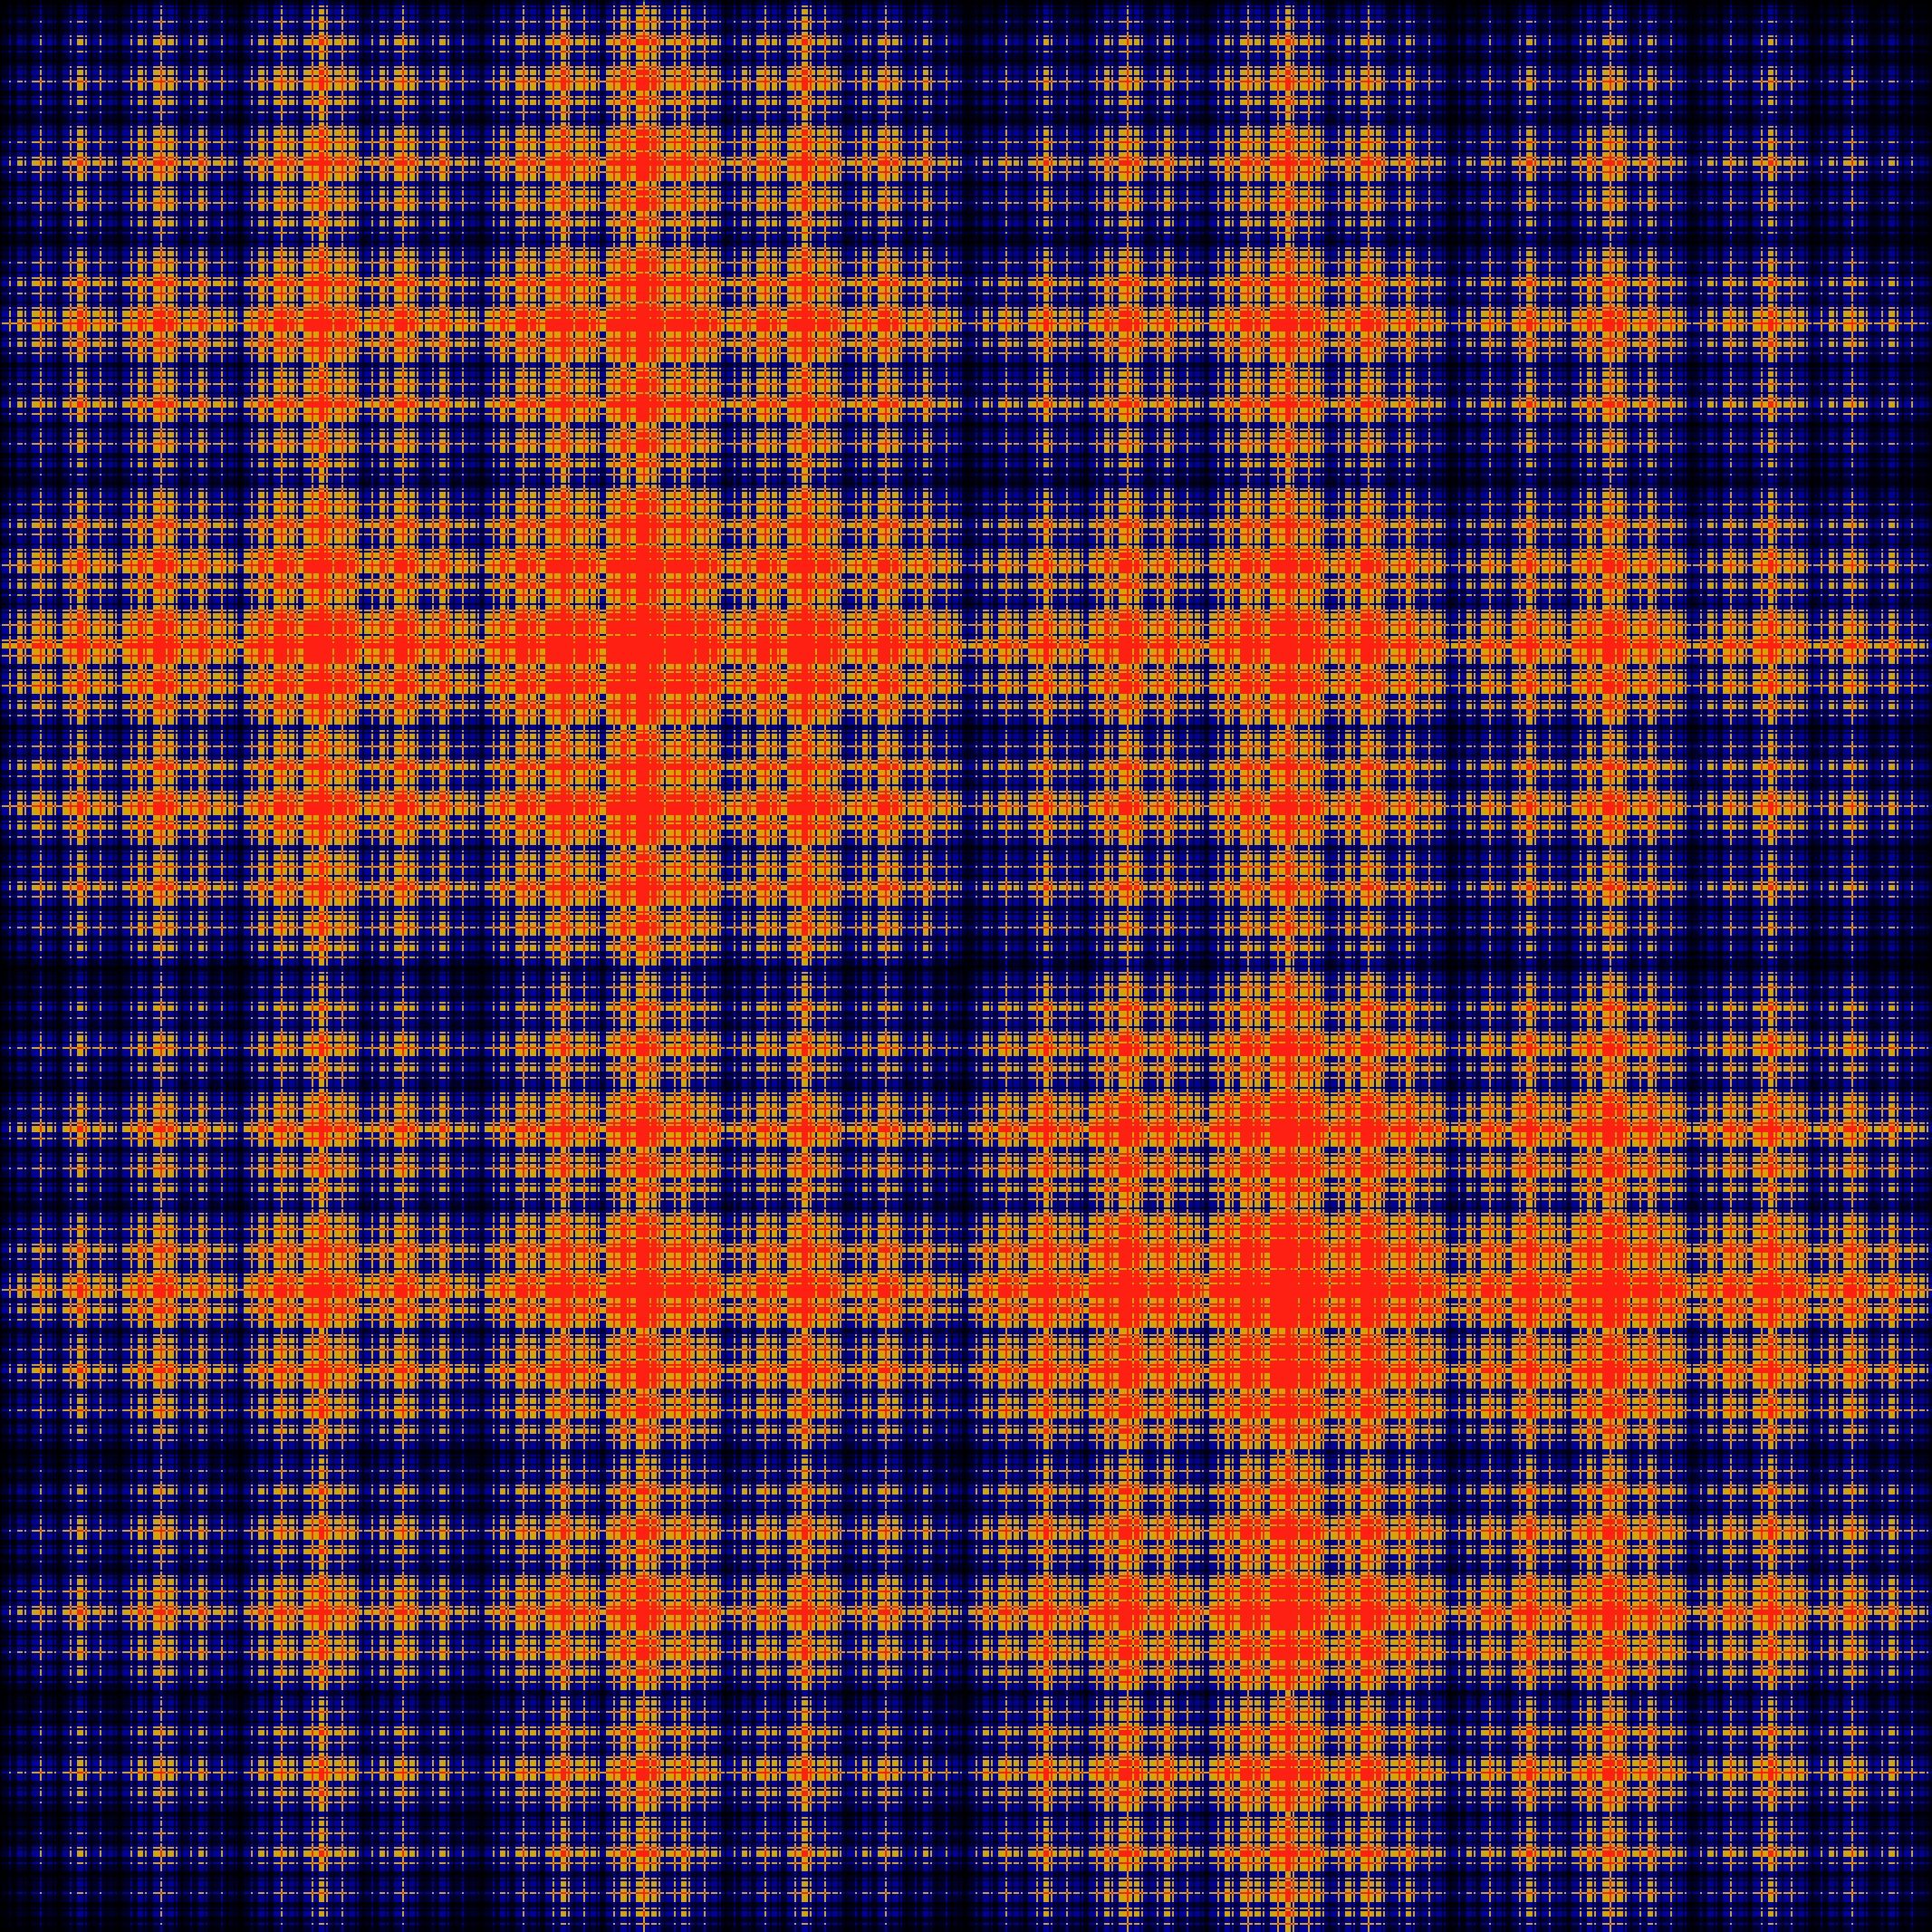
\includegraphics[scale = .25]{Cover}
\end{center}
\frontmatter
\begin{contributors}
\contributor{J. Humpherys}{Brigham Young University}
\contributor{J. Webb}{Brigham Young University}
\contributor{R. Murray}{Brigham Young University}
\contributor{J. West}{University of Michigan}
\end{contributors}
\setcounter{tocdepth}{1}
\tableofcontents

%------------------------------------------------------------------
%The preface, which will presumably be longer in the future
\begin{thepreface}
This lab manual is designed to accompany the book \emph{Foundations of Applied Mathematics}....
\end{thepreface}


%-----------------------------------------------------------------
\mainmatter

%-----------------------------------------------------------------
%Programming Tutorials are in the following sections. They are split into different files dependent upon language

\begin{python}
%Python programming tutorials
\setcounter{chapter}{-1}
\chapter{Getting Started}
%\addcontentsline{toc}{chapter}{Interface}

\objective{An introduction to scientific computing using Python.}

%Latter half of paragraph needs rewording.  Feels rather awkward to read.
This course focuses on the use of computers in solving mathematical problems.  In today's world, many problems that we wish to solve are so large and complex that to solve them by hand would be infeasible.  To be able to effectively use computers to solve these huge problems is becoming a highly demanded skill.  As you work through these labs, you will learn how to use computers to work through complicated problems.  We can say that computation is the muscle of applied mathematics.

These courses will use a powerful yet simple to use programming language called Python as an interface to optimized numerical libraries.  This chapter will walk you through setting up a scientific computing environment based on Python.  All the libraries are freely available on the internet as open source software.

Computation is the muscle of applied mathematics. Regardless of the field of study, inevitably there is a need to utilize computers to answer real world questions.  There exist a variety of tools to tackle these questions.  This course will focus on the use of Python, a powerful, general purpose programming language, to answer these questions.  There are three core libraries for Python that make it viable for scientific computing.  These libraries are SciPy, NumPy, and Matplotlib.  These libraries provide access to many optimized algorithms and to well known libraries such as LAPACK.

\section*{Getting Started}
We will set up our Python environment with the following libraries.
\begin{itemize}
\item Python 2.5 or greater
\item NumPy and SciPy
\item Matplotlib
\item IPython
\item A good editor for editing Python files
\end{itemize}

\noindent A list of editors for python scripts can be found at \url{http://wiki.python.org/moin/PythonEditors}

\subsection*{Python}
\url{http://www.python.org}

Let's begin by setting up Python.  This text recommends the use Python 2.7, but any Python version greater than 2.5 should work just as well.  Download and install the appropriate installation file for your platform.  If you are running Linux, this step is usually not necessary as most Linux distributions ship with Python pre-installed.  NOTE: On Linux, it is highly recommended you install software from your distribution's package repositories.

\subsection*{Numpy and Scipy}
Numpy: \url{http://numpy.scipy.org/}

\noindent Scipy: \url{http://www.scipy.org/}

Numpy is a fundamental library for scientific computating.  It adds the following features to Python.
\begin{itemize}
\item Efficient N-dimensional arrays
\item Very optimized functions designed for working with large data sets
\item High precision calculations
\item Array language features (like MATLAB)
\end{itemize}

SciPy is another python library that uses NumPy to offer the following additional features.
\begin{itemize}
\item Advanced math (signal processing, optimization, statistics, etc)
\item Very optimized functions for large data sets
\item Scikits (similar to toolboxes for MATLAB)
\end{itemize}

We can obtain both libraries from their respective websites.  Be sure to download the version that matches your version of Python.  For instance, if you installed Python 2.7.1, then you will need the numpy-xxxxx-py27.exe install file.  Installation should be quick and easy as NumPy and Scipy will automatically detect your Python installation and configure themselves accordingly.

\subsection*{Matplotlib}
\url{http://matplotlib.sourceforge.net/}

Matplotlib is a 2D plotting library for Python.  It produces publication quality plots and graphs.
For plotting, we will use the Matplotlib library.  The procedure for installing Matplotlib is very similar to that of NumPy and SciPy.  Again, make sure the version you're downloading matches the version of Python that you have installed.

\subsection*{IPython}
\url{http://ipython.org/}

Finally, we will need to install IPython.  IPython can be downloaded from their website.  Users of Windows will also need to download and install the library PyReadline (a straightfoward process that matches the previous two installations).

For those who wish escape the technical details of configuring your own environment, there are several pre-configured python environments available.  One such environment is Enthought.  It offers a free edition that includes these libraries and more.  Another environment is Python(x,y).  These environments include everything needed for this course and much more.  For Linux and Mac OSX users, SAGE also provides a pre-configured environment that includes these libraries.

One additional tool that we will mention is the Spyder Scientific Computing environment.  This tool provides an interface similar to MATLAB.  Though not required for this course, it is worth looking at.  It requires additional libraries to be installed.

\section*{Introducing Python}
Python syntax is very powerful, but is fun and easy to learn.  One day devoted to studying the syntax to Python will be well worth your time.  You should be able to learn and understand most python syntax after a single day.  At the end of this chapter are several helpful resources for learning python.

\subsection*{Data Types}
Computer programs store and manuipate data.  This data is stored in various forms that makes it easy to work with.  Python has native support for several powerful data types.
%Python is dynamically typed.

\subsubsection*{Numeric and Boolean Types}
Python has native support for integers, floats, and complex numbers.  The standard arithmetic operations are supported for each type.
\begin{lstlisting}[style=python]
 a = 15         #an integer
 b = 15.0       #a float
 c = 15+1j      #complex number
\end{lstlisting}

Boolean types have only two possible values: \li{True} or \li{False}.

\subsubsection*{Container Types}
Powerful container types add to the flexibility of Python.  The container types include:
\begin{itemize}
 \item Tuples
 \item Lists
 \item Dictionaries
 \item Sets
\end{itemize}

\paragraph{Tuples}
Tuples are just like lists except that tuples cannot be have items added or removed.  Once created, a tuple can never change.  Why use tuples over lists?  Tuples have less overhead than lists.  


Once a tuple is defined, it cannot be changed (this is referred to as an immutable sequence).  They are represented by parentheses.  Lists are also sequences of objects, but lists are mutable, or changeable.  Lists are represented by square brackets.  Dictionaries store objects in key-value pairs.  Dictionaries are represented by curly braces.  Below are a few examples.
\begin{lstlisting}[style=python]
#Tuples
t = (3,5,6,2, 'this is a tuple') #a tuple with four integers
l = [3,'this is a list', 5 10]
d = {'name':'dictionary', 'value':'Hi There'}
t[0]    #returns 3
l[-1]   #returns 10 (the last item)
d['name']       #returns 'dictionary'
\end{lstlisting}
Note that indexing in Python starts with zero.  That is, the first of item is located at index 0.  Python also allows us to conveniently work backwards from the end of the list using negative indices.

\paragraph{Lists}
Lists are like arrays in that they store ordered sequences of objects.  This datatype is Python's workhorse datatype.  They are incredible useful and efficient.  Mastery of lists will greatly increase your productivity in Python.  The arrays that we will be using later in this course follow the same conventions as lists in Python.  So master lists, and you will be confident working with NumPy arrays!  To create a list we use square brackets around a comma separated list of objects.  They objects can be of any type (they don't all even have to be of the same type).  We initialize a list with 4 objects: an integer, a string, a float and a boolean.
\begin{lstlisting}[style=python]
a_list = [3, 'string', 50.0, True]
\end{lstlisting}
Now, how do we gain access to these elements in the list?  Lists are indexed with integer indices just like arrays. So \li{a_list[0]} will return the first object in the list (the integer \li{3}).  Lists can also be accessed from the end using negative indices (\li{a_list[-1]} returns the boolean \li{True}).

Accessing single elements of the list is great, but what if we what a subset of the list?  This is also very simple.  We can request a subset of any list in Python by slicing the list.  We slice a list using the form \li{a_list[start:end]}.  This will return another list containing the elements of the original list beginning with \emph{start} up to, but not including \emph{end}.  When \emph{start} is 0 or \emph{end} is the -1, we can omit them such as \li{a_list[:3]} and \li{a_list[1:]} because the are implied.  To make a copy of the entire list we can do \li{a_list[:]}.

Now that we can create and slice lists, how do we change the contents of a list?  This is also very simple to do.
\begin{lstlisting}[style=python]
alist = []      #begin with empty list
alist = alist+[1, True] #alist = [1, True]
alist.append(5)           #alist = [1, True, 5]
alist.insert(0,'hi')      #alist = ['hi', 1, True, 5]
alist.extend([0,1,2])     #alist = ['hi', 1, True, 5, 0, 1, 2]
\end{lstlisting}
This listing show how we can add two lists together, append an item at the end, insert an item at a certain index, or extend a list with another list.

Removing items from a list is simple too!  Consider the following listing.
\begin{lstlisting}[style=python]
#alist = ['hi', 1, True, 5, 0, 1, 2]
alist.remove(1)
#alist = ['hi', True, 5, 0, 1, 2]
alist.remove(1)
#alist = ['hi', True, 5, 0, 2]
alist.pop(0)    #returns the item it removed from the list
#alist = [True, 5, 0, 2]
\end{lstlisting}
Those are the basics of Python lists.

\paragraph{Dictionaries}
Dictionaries store data in key-value pairs.  The keys of a dictionary must be unique.  The values can be any data type.

\paragraph{Sets}
Sets are a collection of unordered, unique items.  Very close to the mathematical definition of a set.

\subsubsection*{Functions}
Python functions are defined by the \li{def} keyword.  Notice the colon after the function definition.  This colon tells python to expect a block of code to follow.  Spacing is very important in Python.  Where other languages use brackets to enclose blocks of code, Python uses spacing to define blocks of code.  As such, Python will complain if spacing is not correct or is inconsistent.  This language feature forces correct indentation, making Python code very readable.  Here's an example of a python function.
\begin{lstlisting}[style=python]
def myFunction():
   print "You called?"

myFunction()	#prints: You called? to the console.
\end{lstlisting}

\subsubsection*{Loops and Conditional Statements}
Python also two forms of loops.  The \li{while} loop will execute as long as its test condition evaluates to \li{True}.  The \li{for} loop is used for iterating through lists, tuples, and dictionaries.
\begin{lstlisting}
a = 0
while a is not 10:
   a = a + 1
   print a
print "I'm outside the while loop"
# while loop will continue until a is 10, then print: I'm outside the while loop

for a in [6,5,4,3,2,1,0]:
   print a
   if a == 2:
       print "This is a 2"	#executes if a is 2
   elif a is 5:
       print "I'm a 5 now"	#executes if a is 5
   else:
       print "Still looking..."	#executes if a is anything else
print "I'm outside the for loop"
\end{lstlisting}

\section*{Testing our environment}
We will walk you through some quick tests to demonstrate a working environment.

Start by typing \li{ipython} in your command line.
\begin{lstlisting}
$ ipython
Python 2.7.2 (default, Jun 29 2011, 11:17:09) 
Type "copyright", "credits" or "license" for more information.

IPython 0.11 -- An enhanced Interactive Python.
?         -> Introduction and overview of IPython's features.
%quickref -> Quick reference.
help      -> Python's own help system.
object?   -> Details about 'object', use 'object??' for extra details.

In [1]: 
\end{lstlisting}

Our cursor will be waiting for us to type something.  Lets start by loading the SciPy library.  If we have everything set up correctly, SciPy will import correctly and we will be presented with another prompt.
\begin{lstlisting}[style=python]
In [1]: import scipy

In [2]:
\end{lstlisting}

Let's try making an array.  This will also signal that NumPy is working correctly because arrays are defined in NumPy (NumPy is automatically imported by SciPy).
\begin{lstlisting}[style=python]
In [2]: A = scipy.array([[3,3,3],[2,2,2],[1,1,1]]); print A
Out[2]:
array([[3, 3, 3],
       [2, 2, 2],
       [1, 1, 1]])
\end{lstlisting}

IPython allows us to access the help pages for any function in a quick and intuitive way.  Simply pose your command as a question by appending a \li{?} at the end of the command.  To view the source code of the function (if available), use two question marks. Let's read the help page for scipy.eye. (Note: Outside of IPython, the command is \li{help(scipy.eye)}.)
\begin{lstlisting}
In [3]: scipy.eye?
String Form:   <function eye at 0x8762064>
Namespace:        Interactive
File:             /usr/lib/python2.7/site-packages/numpy/lib/twodim_base.py
Definition:       scipy.eye(N, M=None, k=0, dtype=<type 'float'>)
Docstring:
    Return a 2-D array with ones on the diagonal and zeros elsewhere.

    Parameters
    ----------
    N : int
      Number of rows in the output.
    M : int, optional
      Number of columns in the output. If None, defaults to `N`.
    k : int, optional
      Index of the diagonal: 0 (the default) refers to the main diagonal,
      a positive value refers to an upper diagonal, and a negative value
      to a lower diagonal.
    dtype : data-type, optional
    Returns
    -------
    I : ndarray of shape (N,M)
      An array where all elements are equal to zero, except for the `k`-th
      diagonal, whose values are equal to one.

    See Also
    --------
    identity : (almost) equivalent function
    diag : diagonal 2-D array from a 1-D array specified by the user.

    Examples

    Examples
    --------
    >>> np.eye(2, dtype=int)
    array([[1, 0],
           [0, 1]])
    >>> np.eye(3, k=1)
    array([[ 0.,  1.,  0.],
           [ 0.,  0.,  1.],
           [ 0.,  0.,  0.]])
\end{lstlisting}

\section*{Using Python}
Now that we have a working environment, let's learn how to use in the context of this course.

We will be writing and executing many programs written in Python.  How do we accomplish this?  Python programs are contained in files using a *.py extension.  Any number of functions can be contained in these files.  They are executed from the commandline using the following command (where \li{program.py} is the name of the program we want to execute):
\begin{lstlisting}
$ python program.py
\end{lstlisting}

We can treat our programs as libraries (as you will see near the end of this chapter with the benchmarking function).

\section*{Using SciPy}
SciPy is organized into base library with other libraries to handle special features.  We can import these other libraries whenever we need to use them.  Most of the functions we use in this book come from the scipy, linalg, and sparse libraries. The different libraries available in SciPy are:
\begin{lstlisting}
scipy.cluster: Clustering package
scipy.constants: Constants
scipy.fftpack: Fourier transforms
scipy.integrate: Integration and ODEs
scipy.interpolate: Interpolation
scipy.io: Input and output
scipy.linalg: Linear algebra (imported as la)
scipy.maxentropy: Maximum entropy models
scipy.misc: Miscellaneous routines
scipy.ndimage: Multi-dimensional image processing
scipy.odr: Orthogonal distance regression
scipy.optimize: Optimization and root finding
scipy.signal: Signal processing
scipy.sparse: Sparse matrices (imported as spar)
scipy.sparse.linalg: Sparse linear algebra (imported as sparla)
scipy.spatial: Spatial algorithms and data structures
scipy.spatial.distance: Distance computations
scipy.special: Special functions
scipy.stats: Statistical functions
scipy.weave: C/C++ integration
\end{lstlisting}

When we use SciPy in book, it will always be imported as follows. This python statement imports all the main SciPy methods for use and make them available in the \li{sp} object.
\begin{lstlisting}
import scipy as sp
\end{lstlisting}

To use the SciPy's linear algebra library, we use the following import statement.  After this statement, all the linear algebra methods of SciPy will be available under the \li{la} object.
\begin{lstlisting}
import scipy.linalg as la
\end{lstlisting}

\section*{Matplotlib}
SciPy does not provide methods for generating graphics (plots, graphs, etc.).  Matplotlib is a libary written for Python to provide a MATLAB like plotting environment.  If you are familiar with plotting in MATLAB, Matplotlib should be easy to use.  In this course we will be importing Matplotlib as follows.  Again note that after importing \li{matplotlib.pyplot}, the methods will available under the \li{plt} object.
\begin{lstlisting}
import matplotlib.pyplot as plt
\end{lstlisting}

\section*{A Note on Floating Point Arithmetic}
In mathematics we expect that the difference between two equal quantities to be zero.  For example, $10 - 10 = 0$.  floating point arithmetic isn't always so precise - altering the previous expression to $e^{log(10)} - 10 = 0$ changes nothing on paper, but try putting it into IPython:

\begin{lstlisting}
: 10 - 10
0
: scipy.exp(scipy.log(10))-10
1.7763568394002505e-15
\end{lstlisting}

This is due to floating point arithmetic. Floating point numbers do not have arbitrary precision: they only occupy a certain amount of memory.  For numbers with long decimal expressions or irrational numbers, there will inevitably be a loss of precision because of this memory constraint.  Although these errors will generally be small it is important to understand this limitation of numerical computation. The intricacies of floating point arithmetic will be further developed in Volume II of this work.

Another thing to watch out for is integer division.  It is common in programming to return an integer when dividing two integers.  Type \li{a \= 1/2} into IPython.  What do you expect the value of \li{a} to be?  If you're thinking 0.5, that is incorrect.  Type \li{print a}.  Notice that it returns \li{0}.  This is because both \li{1} and \li{2} are integers, so dividing them produces \li{0}.  To get 0.5 (a floating point number), we need to tell Python that it should treat \li{1} or \li{2} as a float.  Type \li{b = 1.0/2; print b}.  Now the result is 0.5.
There are two ways to force Python to always return a float when dividing.  First we can run a script and pass the \li{-Qnew} option to the Python interpreter.  Second, we can import the following at the top of each script where we wish to use only true division.
\begin{lstlisting}
from __future__ import division
\end{lstlisting}

%\section*{Timing Code}
%As a final note, there are several methods for timing code. This will be important, since throughout this book we stress understanding the intrinsic complexity of different methods for solving problems. We have provided a \li{timer} class (which you will have to download), that makes the python timing interface easier to use. 

\section*{Benchmarking}
Before we continue, there is one more thing we need to discuss.  Throughout this book, you will be asked to compare execution times of different pieces of code.  IPython allows us to easily do this from the console using the \li{\%timeit} command.
\begin{lstlisting}
: %timeit [a**3 for a in range(30)]
100000 loops, best of 3: 11.5 us per loop
\end{lstlisting}
The \li{\%timeit} command wraps a Python module called \li{timeit}.  This module will execute a statement many times, timing it each time, and report the best execution time.  The reason for multiple timed executions is to account for random system variances which may affect the performance of function.  Also note that \li{timeit} will disable Python's garbage collector during the tests (the garbage collector is how Python automatically manages memory).  We see above that out of 3 million executions (100000 loops repeated 3 times), the fastest time per loop was 11.5 microseconds.  We can even time the execution of functions.

The problem with \li{\%timeit} is that it is only defined inside ipython.  The authors of this book have written a Python module that wraps \li{timeit} into an easy to use Python context.  Please save the following code into an easily accessible file.

\lstinputlisting[style=python, style=fromfile, name=mytimer.py]{mytimer.py}

The reader is not expected to understand the above function (though it would be worthwhile study it).  It uses a feature of Python called contexts.  Consider the following code.
\begin{lstlisting}
from mytimer import timer
with timer() as t:
    t.time(myFunction, arguments)
    t.printTimes()
\end{lstlisting}

Python contexts are used via the \li{with} keyword.  In the above code, we initialize the \li{timer()} context which returns to us a \li{timer()} object bound to the variable \li{t}.  Inside the block, we can execute anything.  If we wish to time a specific function we call the \li{time()} method of \li{t}.  The \li{time()} method accepts a function and its parameters and returns the best execution time (in the form of a string) in the following form:
\begin{lstlisting}
myFunction finished in 0.00283s (1 loops, repeated 3 times): 0.00283s per loop (with gc.disable())
\end{lstlisting}

\section*{Helpful Resources}
\subsubsection*{Python}
\noindent \emph{Dive into Python}:  This python book is a great resource for beginning to understand python.  It is available for for free download. \url{http://diveintopython.org/}

\noindent \emph{Non-Programmer's Tutorial for Python}: \url{http://en.wikibooks.org/wiki/Non-Programmer\%27s_Tutorial_for_Python}

\noindent \emph{The Python Tutorial}: Written by the creator of Python. \url{http://docs.python.org/tutorial/}

\subsubsection*{NumPy and SciPy}
\noindent \emph{NumPy Reference Manual}: \url{http://docs.scipy.org/doc/numpy-1.6.0/reference/}

\noindent \emph{SciPy Reference Manual}: \url{http://docs.scipy.org/doc/scipy-0.9.0/reference/}

\noindent \emph{NumPy for MATLAB Users}: Comparing and contrasting Python and MATLAB. \url{http://www.scipy.org/NumPy_for_Matlab_Users}

\noindent \emph{MATLAB to NumPy translation table}: A table with MATLAB commands and their equivalent NumPy functions.   \url{http://mathesaurus.sourceforge.net/matlab-numpy.html}

\noindent \emph{NumPy and SciPy Cookbook}: \url{http://www.scipy.org/Cookbook}

\noindent \emph{Introduction to Arrays}: Very informative introduction the SciPy arrays. \url{http://pages.physics.cornell.edu/~myers/teaching/ComputationalMethods/python/arrays.html}

\subsubsection*{Matplotlib}
\noindent \emph{Matplotlib User Guide}: \url{http://matplotlib.sourceforge.net/contents.html}

\noindent \emph{Matplotlib Examples}: Useful for seeing the python code that generate certain plots. \url{http://matplotlib.sourceforge.net/examples/index.html}





\lab{Algorithms}{Matrix Operations and Algorithmic Complexity}{Matrices and
Complexity}
\objective{This lesson explains basic matrix operations in Python.}

%Make a note command

Matrices form the core data structure of NumPy and SciPy.  Thus, we will explore
the ways one can manipulate matrices in Python.

Before we begin, we make a few important comments about how Python works with matrices. First of all, matrices can be represented in NumPy in two ways.  NumPy has a matrix
datatype and an array datatype.  Matrix objects are a special case of the array
object.  The main differences are that the matrix object allows for a clearer,
more matlab type syntax.  In this book, we will use arrays because most functions in python use arrays as input. We can easily convert arrays to matrices using the asmatrix()
method.  As such, all future references to matrices in the context of NumPy will
mentioned as arrays (a matrix being a 2D array).  When using arrays it is important to be sure that the dimensions are compatible.

We also note that arrays are stored row by row. This is called Row-Major. This is the opposite of MATLAB, which is Column-Major.

Finally, with all code examples in this book we assume that you have already imported the SciPy library (type \texttt{import scipy as sp} when you first open ipython).

To begin we will work with vectors. We will demonstrate a variety of methods to
create vectors. You should follow these demonstrations on your own computer and
experiment as you go.  Vectors are at least one dimensional arrays.  There are
several ways to create vectors in Python.  Try the following in IPython:

\begin{lstlisting}
: a = sp.array([1,2,3,4]); a
array([1, 2, 3, 4])
\end{lstlisting}

Notice the square brackets and the commas.  The square brackets denote a list in
Python with values separated by commas.  This is a row vector.  The \texttt{; a}
is responsible for printing the current value of \texttt{a}.  How do we make a
column vector?  We simply pass the array() method a list of lists containing a
single value each.
\begin{lstlisting}
: b = sp.array([[3],[4],[6],[1]]); b
array([[3],
       [4],
       [6],
       [1]])
\end{lstlisting}

We can also use the hstack() and vstack() methods (meaning horizontal stack and
vertical stack).
\begin{lstlisting}
: a1 = sp.hstack([5,6,7,8])
: b1 = sp.vstack([9,0,1,2])
\end{lstlisting}

We combine vectors together by placing two or more of equal dimension inside
square brackets. The technical term for this is concatenation.  Remember that
the dimensions of each array must match.  Try the following.
\begin{lstlisting}
: c = sp.concatenate((b,b1), axis=1); c
\end{lstlisting}

There are several methods to automate vector creation. For example, we can build
a vector of consecutive values using the \texttt{arange()} method.

\begin{lstlisting}
: sp.arange(5)
\end{lstlisting}

Notice how the values start at zero and increment up to, but \emph{not}
including 5.  This is standard Python behaviour.  The \texttt{arange()} method
also allows us to specifiy step size
This syntax also allows us to specify step size:

\begin{lstlisting}
: sp.arange(1,3,step=0.5)
\end{lstlisting}

We can similarly use negative step sizes (note that the starting must be greater
than the endpoint).

\begin{lstlisting}
: sp.arange(3,1, step=-.5)
\end{lstlisting}

A related function is called \li{linspace()}. It allows us to specify two
endpoints and the number of equidistant values we want between the two.  Unlike
\li{arange()}, \li{linspace()} will always include both endpoints.

\begin{lstlisting}
: sp.linspace(1,2,5)
\end{lstlisting}

The \li{plot()} function uses two vectors to create a graph, the first vector
representing $x$-values and the second representing the corresponding
$y$-values.  To use \li{plot()}, we need to import the Matplotlib library.  As
an example we plot a line of slope two using the following commands (See figure
1.1):

\begin{lstlisting}
: import matplotlib.pyplot as plt
: x = sp.linspace(-2,2,20)
: plt.plot(x,2*x)
: plt.show()    
\end{lstlisting}

\begin{figure}
\begin{center}
        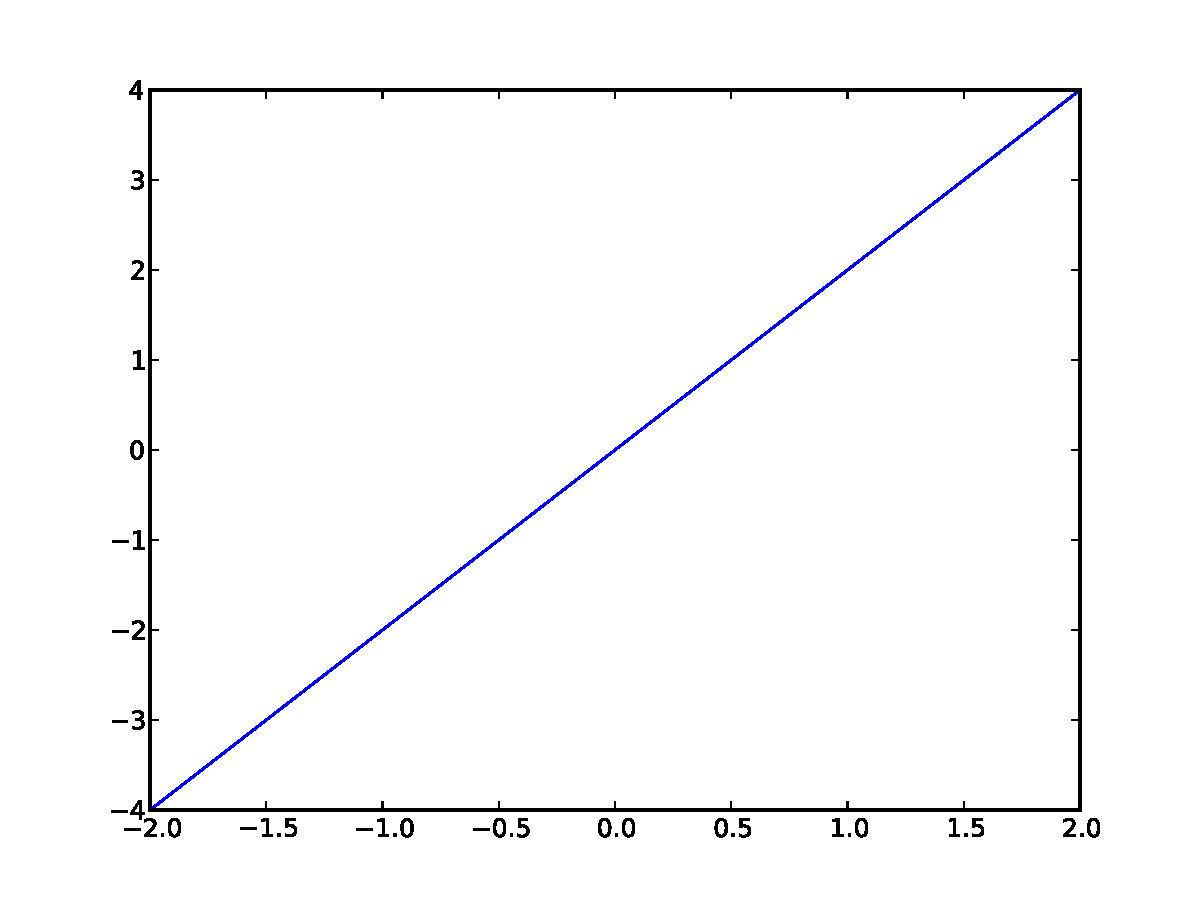
\includegraphics[scale=0.5]{./Figures/graph.pdf}
        \caption{A simple graph}
\end{center}
\end{figure}

By typing \li{plt.plot?} into the command line we can find the exact syntax and
options for the \li{plot()} function. For example we can type {\tt
plot(x,2*x,'r*')} to plot red star data points instead of a line.

\begin{problem}
Plot a line with slope three with black diamond data points. Plot for the domain
$x \in [-5,5]$. 
\end{problem}

Creating is done by concatenating vectors in the correct manner. For example:

\begin{lstlisting}
: sp.array([[1, 2, 3],[4, 5, 6],[7, 8, 9]])
\end{lstlisting}

\begin{problem}
Create a matrix showing the times table from 1 to 6. Do not enter each number
manually. Instead, create a variable \li{x = sp.arange(1,7)} and let the rows
of the matrix be multiples of $x$.
\end{problem}

Another technique for creating matrices is using outer products. An outer
product is the method of multiplying two vectors to get a matrix. For example,
if we want to make a matrix that is two repeated rows of the vector 1:5 we can
do the following:

\begin{lstlisting}
: sp.vstack([1,1])*sp.arange(1,6)
\end{lstlisting}

Here we are multiplying a $2 \times 1$ vector and a $1 \times 5$ vector, which
yields a $2 \times 5$ matrix. The two rows are identical since the entries of
the first vector are all ones.

%SciPy has an outer product function
\begin{problem}
Create the same matrix from problem 2, using outer products this time. This
implementation, although perhaps more difficult to conceptualize, makes for much
more concise code.
\end{problem}

You can also combine matrices in the same way as vectors, as long as the
dimensions match correctly, i.e. the same number of rows or the same number of
columns. Try the following:

\begin{lstlisting}
: D = sp.hstack((b, c))
: E = sp.concatenate([D.T, sp.vander(sp.arange(1,5))])
\end{lstlisting}

Here we used the \li{vander()} method, which accepts a vector of length $n$ and
creates an $n \times n$ matrix. The columns of this matrix are powers of the
input vector (evaluated point-wise). More information about the \li{vander()}
method by typing \li{sp.vander?}.

To briefly review, vectors are built using the square brackets, with semi-colons
to build columns and spaces to build rows. Matrices are built in exactly the
same way, using vectors or matrices instead of individual numbers.

Often while writing code it is necessary to know information about the
properties of an array.  The matrix properties can be accessed as follows.

\begin{lstlisting}
: E.ndim        #dimension of E
: E.nbytes      #size of E in memory (bytes)
: E.size        #total area of E (the product of the dimensions)
: E.shape       #size of E in each dimension
\end{lstlisting}

For this next problem we will need to read an array from a file.  SciPy provides
a method for loading data from text files.  We are going to load \li{bucky.csv}
as an array.
\begin{lstlisting}
: bucky = sp.loadtxt("bucky.csv", delimiter=",")
\end{lstlisting}

This array represents the connections between vertices of a truncated
isocahedron.  This soccer ball like shape is found in certain types of carbon
molecules known as fullerenes (specifically $C_{60}$, shown in shaped 
 
%---REMOVE PROBLEM?---
\begin{problem}
The bucky matrix represents the connections
between the vertices of a truncated isocahedron. This structure matches both the
structure of a standard soccer ball, and also of certain types of carbon
molecules known as fullerenes (specifically $C_{60}$, shown
in~\ref{fig:fullerene}). It is also related to the structure of the geodesic
dome. Find the size of this matrix.
\end{problem}

\begin{figure}[h!]
\begin{center}
\label{fig:fullerene}
\includegraphics[scale = .2]{./Figures/C60a.png}
\caption{The structure of the $C_{60}$ molecule.}
\end{center}
\end{figure}


To access information in an array, you put the index you wish to access inside
square brackets after the variable name. This works for both variable assignment
and retrieval.  Remember that indices start at zero in SciPy.

\begin{lstlisting}
: rand_mat = sp.random.randint(10, size=(3,5))
: rand_mat[0,0]
: rand_mat[2,2] = 37
\end{lstlisting}

The colon operator is used to retrieve an entire row or column from an array. 
For example, enter the following to get the third column of an array:

\begin{lstlisting}
: rand_mat[:,2]
\end{lstlisting}

We similarly retrieve the first row:

\begin{lstlisting}
: rand_mat[0,:]
\end{lstlisting}

Note that each retrieved row or column is returned as a single dimensional array
(meaning that row or column loses it meaning). If we want to retain the retrieved row as a column or row we can write instead \li{rand_mat[:,[2]]}.

It is also possible to retrieve multiple columns or rows at once. For example,
we retrieve the second and fourth columns of an array by entering:
\begin{lstlisting}
: rand_mat[:,[1,3]]
\end{lstlisting}

We list the entries of an array as a single dimensional array using the {\tt
flatten()} method.

\begin{lstlisting}
: rand_mat.flatten() #flattens along the rows (C like arrays)
: rand_mat. flatten('F') #flattens along the columns (Fortran like arrays)
\end{lstlisting}

The following line tells Python to retrieve the entries in the second row, from
the second column to the end:

\begin{lstlisting}
: rand_mat[1,1:]    
\end{lstlisting}

Deleting a row or column can be done by using the \li{delete()} method.  The
last argument is the axis along which to delete.  If the deletion axis is not
specified, then the array will be flattened before being returned. Here we
remove the column at index 1.
\begin{lstlisting}
: sp.delete(rand_mat, 1, 1)
\end{lstlisting}
 
\begin{problem}
Try to assign a vector of incorrect size to a piece of a matrix. What happens?
Also, try to concatenate two matrices that don't have matching dimensions. What
error message do you get? It is important to learn how to read error messages
for troubleshooting purposes.
\end{problem}

Numerical operations are by default done element-wise on arrays.  A common
mistake is to use \li{*} for matrix multiplication.  This simply multiplies
each element by a constant.  To perform matrix multiplication, SciPy provides the \li{dot()} method.  To take the transpose of an array, use the \li{.T} property.  Observe the behavior of the array operations.
\begin{lstlisting}
: b = sp.vstack([8,0,2])
: c = sp.vstack([4,2,1])
: b+c
array([[12],
       [ 2],
       [ 3]])
: b-c
array([[ 4],
       [-2],
       [ 1]])
: A = sp.array([0,4,5,4,0,2,9,4,6]).reshape((3,3))
: A*b #b is a column vector, so each row is multiplied by a constant
array([[ 0, 32, 40],
       [ 0,  0,  0],
       [18,  8, 12]])
: A*b.T #b.T is a row vector, so each column multiplied by a constant
array([[ 0,  0, 10],
       [32,  0,  4],
       [72,  0, 12]])
: sp.dot(A,b)
array([[10],
       [36],
       [84]])
: sp.power(A,2) #this is A^2
array([[ 0, 16, 25],
       [16,  0,  4],
       [81, 16, 36]])
: A/2 #notice that type is perserved.  This is integer division
array([[0, 2, 2],
       [2, 0, 1],
       [4, 2, 3]])
: A/2. #divide by a float yields an array of floats.
array([[ 0. ,  2. ,  2.5],
       [ 2. ,  0. ,  1. ],
       [ 4.5,  2. ,  3. ]])
\end{lstlisting}

The majority of elementary functions, such as \li{sin}, \li{cos}, \li{exp}, etc. act element-wise on arrays as well.  In fact, for any operation in SciPy, expect it to act element-wise unless otherwise noted.  For example:
\begin{lstlisting}
: sp.sin(sp.arange(4)*sp.pi/4)
array([ 0.        ,  0.70710678,  1.        ,  0.70710678])
\end{lstlisting}

Also, as a matter of reference, raising a value to a power is done using \li{**}. This is an convention from older programming languages that has carried over.

There are a variety of functions that let us summarize information about a given
array. For example, the \li{sum()} function returns the sum along a given axis of an array.  When an axis is not specified, all elements in the array are summed together.
\begin{lstlisting}
: B = sp.arange(9).reshape((3,3))
: sp.sum(B) #all entries are summed together
36
: sp.sum(B, axis=0) #sum each column
array([ 9, 12, 15])
: sp.sum(B, axis=1) #sum each row
array([ 3, 12, 21])     
\end{lstlisting}

Some other functions that summarize information about the entries of an array
are contained in the Table 1.1. Note that each of these functions reduces the
size of the matrix (which makes sense, since they are summarizing functions).
These functions work across columns by default, although most of them allow you
to specify an axis to work across.


\begin{table}[h!]
\begin{center}
	\begin{tabular}{|l|p{4cm}|l|}

    \hline

    Function & Description & Usage\\

    \hline

    \li{max} & Returns maximum entries & A.max(axis)\\

    \li{min} & Returns mimimum entries & A.min(axis)\\

    \li{mean} & Returns the mean & A.mean(axis)\\

    \li{scipy.median} & Returns the median & sp.median(A, axis)\\
    
    \li{std} & Returns the standard deviation & A.std(axis) \\

    \li{scipy.diff} & Returns the differences between entries & sp.diff(A, axis)\\
    
    \li{prod} & Returns the product of entries & A.prod(axis)\\
    
    \li{any} & Returns 1 if there are non-zero entries, zero otherwise & A.any(axis)\\
    
    \li{all} & Returns 1 if all entries are non-zero, zero otherwise & A.all(axis)\\

   \li{nonzero} & Returns indices of non-zero entries & A.nonzero(axis)\\

   \li{scipy.linalg.norm} & Returns the norm & norm(A, order)\\ 

    \hline

    \end{tabular}
\end{center}
\caption{Various summarizing functions}
\end{table}

These functions can be incredibly useful. For example, suppose that we want to
estimate the derivative of $sin(x^2)$. A simple approximation for a derivative
is
\[
f'(x) \approx \frac{f(x+h) - f(x)}{h}
\]

Presumably this approximation is good when $h$ is small. We use the \li{diff()}
function to perform this approximation using the following code:

\begin{lstlisting}
: h = .001
: x = sp.arange(0,sp.pi,h)
: approx = sp.diff(sp.sin(x**2))/h
\end{lstlisting}

We have just approximated the derivative of $\sin{x^2}$ at several thousand points between $0$ and $\pi$.  The approximated derivatives are stored in the array \li{approx}.  Now let's compute the actual derivative at each point using the formula:
\[
f'(x) = 2x cos(x^2)
\]
\begin{lstlisting}
: actual = 2*sp.cos(x**2)*x;
\end{lstlisting}

Plot the approximated derivative and the actual derivative on two different
plots.  They should look almost identical.
\begin{lstlisting}
: from matplotlib import pyplot as plt
: plt.figure(1) #create an empty figure
: plt.subplot(211) #create an empty subplot in figure
: plt.plot(x, approx)
: plt.subplot(212) #create another subplot in same figure
: plt.plot(x, actual)
: plt.show()
\end{lstlisting}

\begin{problem}
Now use the \li{max()} command to find the maximum difference between the estimated derivative and the actual derivative
(the dimensions will not match exactly (why?);  fix this by removing
the last entry from one of the vectors).  Try plotting the approximation, actual deriviatives, and the error on the same graph.  What does it look like?
\end{problem}

\begin{problem}
The command \li{sp.rand()} returns an array of a specified shape with values ``randomly" selected from a uniform distribution between zero and one. Create a  vector with ten thousand entries using this command. The theoretical values for the mean($\mu$)
and standard deviation($\sigma$) of a uniformly distributed random variable
between $a$ and $b$ are
\begin{align*}
\mu &= \frac{a+b}{2} \\
\sigma &= \frac{b-a}{\sqrt{12}}
\end{align*}
These values are calculated using moment-generating functions. Use the 
\li{mean()} and \li{std()} methods on the vector you created earlier. How do these compare to the theoretical values?
\end{problem}

The canonical problem in linear algebra is solving the equation $Ax = b$ for x,
where $A$ is an $n \times n$ matrix and $b$ is a  $1 \times n$ vector.  One method for solving this equation is by calculating the matrix inverse of $A$ ($A^{-1}$) and multiplying $A^{-1}b$.  To find the inverse of an array, use the \li{linalg.inv()} method.
For example, we create a random system $Ax =b$ and solve it using the \li{inv()} method (you may check the calculations by hand):

%Excellent demonstration but needs a bit of work
\begin{lstlisting}
: A = sp.array([1,5,2,3,5,1,4,7,2]).reshape((3,3))
: b = sp.vstack([1, 3, 11./3])
: from scipy import linalg as la
: sol = sp.dot(la.inv(A),b); sol
array([[ 0.66666667],
       [ 0.33333333],
       [-0.66666667]])
\end{lstlisting}

Recall that a norm is a measurement on the size of a vector.  For example, the
Euclidean norm measures the straight line distance from the origin to the
``end'' of a vector.

\[
\norm{x} = \sqrt{x_1^2 + ... + x_n^2}
\]

If the norm of the difference of two vectors is close to zero, then they are
good approximations of each other.  The \li{linalg.norm()} function calculates the
euclidean norm of an input vector, and thus we use it to verify that our
approximation of the derivative is close to the actual derivative:
% We then verify that we have solved the system by comparing \li{A*sol} and
%\li{b} using the \li{norm} function:
\begin{lstlisting}
: la.norm(b-sp.dot(A,sol))
5.5288660751834285e-15
\end{lstlisting}

However, computing the inverse of a large matrix is difficult.  Not only that, but not all matrices have inverses.  There is a much more efficient and general way to solve $Ax=b$ in SciPy.  This method is similar to the backslash method found in MATLAB.  It is the \li{linalg.solve()} method. Compare the results obtained with the \li{linalg.solve()} method to those of the \li{linalg.inv()} method.
\begin{lstlisting}
: sol2 = la.solve(A,b); sol2
array([[ 0.66666667],
       [ 0.33333333],
       [-0.66666667]])
: la.norm(sol2-sol)
4.5775667985222375e-16
\end{lstlisting}

We mentioned that the backslash operator is more efficient than using the
function \li{inv}, meaning it returns a result faster. Create the following script to compare the efficiency of each method:

\begin{lstlisting}
import scipy as sp
from scipy import linalg as la
from timer import timer

def invMethod(A, b):
    return sp.dot(la.inv(A),b)

def solveMethod(A, b):
    return la.solve(A,b)
    
n = 300
A = sp.rand(n)
b = sp.rand(n,1)

with timer(repeats=3, loops=10) as t:
	t.time(invMethod,A,b)
	t.time(solveMethod,A,b)
	t.printTimes()
\end{lstlisting}

Now run the script. You should notice a significant difference in execution time
(you may need to scale $n$ appropriately). Are you surprised that \li{invMethod()} is significantly slower than \li{solveMethod}?  Specifically, SciPy uses the
the LU factorization and backwards substitution to solve the linear system
without any matrix inversions. %check validity

The \li{linalg.solve()} method can also be used to solve several systems at once. For example:

\begin{lstlisting}
: c = sp.rand(n, 1)
: la.solve(A, sp.c_[b,c] #sp.c_[] concatenates column vectors
\end{lstlisting}

%Explain scripts
You might now be asking why we would want to do this. We can answer this by
investigating the time it takes to solve two systems. Open a new script file and
write the following:

\begin{lstlisting}
import scipy as sp
from timer import timer
n = 3000
A = sp.rand(n,n)
b = sp.rand(n,1)
c = sp.rand(n,1)

def multSys(A, *col_vecs):
    return la.solve(A, sp.hstack(col_vecs))
    
def singSys(A, *col_vecs):
    return [la.solve(A, x) for x in col_vecs]

with timer(repeats=3, loops=100) as t:
    t.time(multSys,A,b,c)
    t.time(singSys,A,b,c)
    t.printTimes()
\end{lstlisting}

This script creates a random $3000 \times 3000$ matrix, and two random $3000
\times 1$ vectors (you can experiment with different sizes of matrices and
vectors). It then solves the two systems of equations twice, once using two
backslash commands and the other using only one. Remember that the semi-colons
suppress the output in the script.

Now execute this script. You should notice that the first method takes about
twice as long as the second method. This is because the backslash method uses
the LU decomposition, and in the second method it only has to execute this
factorization once. This highlights the importance of understanding the
algorithms that python uses: we can solve problems much faster if we understand
what python is doing.

A number of other important operators that you will need are found in Table 1.2.
{\footnotesize
\begin{table}[h!]
\begin{center}

    \begin{tabular}{|l|p{4cm}|l|}

    \hline

    Method & Description & Usage \\

    \hline

    \li{linalg.inv()} & Matrix inverse & la.inv(A)\\

    \li{rank()} & Rank & sp.rank(A)\\

    \li{linalg.norm()} & Norm (default: 2-norm) & la.norm(A, ord)\\

    \li{linalg.expm()} & Matrix exponential & la.expm(A) \\

    \li{linalg.det()} & Determinant & la.det(A)\\

    \li{linalg.eig()} & Eigenvalue decomposition & la.eig(A)\\
    
    \li{linalg.svd()} & Singular value decomposition & la.svd(A)\\
    
    \li{linalg.lu()} & LU decomposition & la.lu(A)\\
    
    \li{linalg.qr()} & QR factorization & la.qr(A)\\
    
    \li{linalg.cholesky()} & Cholesky factorization & la.cholesky(A)\\

    \hline

    \end{tabular}
	\caption{Useful matrix operations}
\end{center} 
\end{table}}

%Explain better
\begin{problem}
The \li{linalg.lstsq()} method can be also used to solve overdetermined systems. This is
sometimes also known as the least squares method. The formula is $(A^TA)^{-1}A^T*b$.
Create a script to verify numerically that the \li{linalg.lstsq()} method and the least squares formula yield the same result. Hint: Use the \li{linalg.norm()} function to verify equality, as we did with \li{linalg.inv()} and \li{linalg.lstsq()}.
\end{problem}

\lab{Algorithms}{Building Matrices, Sparse Matrices and Algorithmic Complexity}{Matrices and Complexity, cont.}

\objective{This section explains how to create specific types of large matrices. It also introduces the concept of temporal complexity. Finally, it explores SciPy's special methods for working with sparse matrices.}

\section*{Temporal Complexity}

%{\bf The next two paragraphs are an alternate description of Big O, designed as a more intuitive approach, to help with Vol I (a more technical explanation would be in Vol II). Let me know what you think...}

%I am not sure that this is clear or precise enough.  I think that the previously written stuff with some easier problems may be better...

One of the most important questions in scientific computing is: How long will this operation take?  The concept of temporal complexity attempts to answer this question by determining how much time a function needs to operate on a given size of input.  For example suppose calculating the inverse of a matrix of size $n$ requires the following number of calculations.
%For this reason we often discuss algorithms in terms of their temporal complexity, which describes how long an operation takes in terms of the size of the input. For example, suppose calculating the inverse of a matrix of size $n$ requires the following number of calculations:
\[
f(n) = \frac{3n^3}{2} + 75n^2 + 250n + 30
\]
What is the most important part of this expression? When our input gets very large the only relevant term in this equation is $n^3$. For this reason we say that $f(n) \in O(n^3)$, or more commonly that $f(n)$ is $O(n^3)$ (spoken ``Big O of n cubed'' or ``Order of n cubed"). This notation is borrowed from analysis. This notation captures the salient behavior of our temporal complexity, or more precisely the growth rate we can expect of the execution time of our algorithm. We will discuss this concept later, but this is a simple introduction to the notion of complexity and Big O. Spatial complexity is the amount of memory an algorithm uses, and is defined similarly. 

\begin{comment}

Now that we have begun to study some more complex MATLAB expressions, it is prudent to have a basic notion of the complexity of the operations we are interested in executing.  Complexity theory is the study of the difficulty of computational problems.  What makes computing the sum of two integers easy, and what makes computing the inverse of a large matrix so difficult?  There is an entire field dedicated to answering such questions; in this work we only do a cursory examination to communicate the basic ideas and vocabulary.
	
	To begin, we use an example to illustrate what we are trying to accomplish.  There are occasions when one is willing to sacrifice precision in order to focus on more important features of the object of study.  For example, $f(x) = x^3 + \frac{sin(20x)}{10}$ produces a cubic function with a slight wobble.  In some applications that wobble may be a crucial detail, but in many cases the wobble will be irrelevant and only serves to distract from the salient features of the function.  We extend this example to algorithms.

	An algorithm is an ordered set of instructions.  Something simple like a recipe to bake a cake is an algorithm, but the only algorithms you will be dealing with here are MATLAB operations and programs.  To describe the complexity of an algorithm we use asymptotic notation called ``Big O.''  Big O makes us focus on salient features of the complexity of an algorithm while at the same time suppressing unnecessary details, much like we ignored the sine wobble in the previous example.  It has been said that using Big O is ``the art of knowing where to be sloppy and where to be precise.''
	
	With that introduction, we define Big O:
	
\begin{theorem}
	$f(x) = O(g(x))$ if and only if $\exists$ M $\in \mathbb{N}, x_0 \in dom(f)$ such that $|f(x)| \le M|g(x)|$ $\forall x > x_0$
 \end{theorem}
 
 This is an abuse of notation, we really should be saying that $f(x) \in O(g(x))$ since $O(g(x))$ is not a function but an equivalence class of functions.  Lamentably, using $=$ has become embedded into the culture, so there is not much to be done except make a note of the correct notation and move along.
 
 \begin{example}
 $x^2 = O(x^3)$ since $x^2 < x^3$ when $x > 1$
 \end{example}
 
 \begin{example}
 $x^3 + 3x^2 + x + 4 = O(x^3)$ since $x^3 + 3x^2 + x + 4 < 10x^3$ when $x > 1$
 \end{example}
 
  \begin{example}
 $x^2 + 10000x = O(x^2)$ since $x^2 + 10000x < 100000x^2$ for all x.
 \end{example}
 
You can see that when we talk about Big O of polynomials, we are simply dropping off lower order terms and ignoring coefficients.
% 
% (These problems may be too challenging)
% \begin{problem}
% Show that $O(\log{x}) \subset O(x) \subset O(x\log{x})$
% \end{problem}
% 
% \begin{problem}
% Show that $O(x^k) \subset O(x^{k+1})$
% \end{problem}
% 
% \begin{problem}
% Show that $O(x^p) \subset O(2^x)$ for all $p \in \mathbb{N}$
% \end{problem}
% 
	What does this have to do with computer programs?  Every algorithm executed on a computer corresponds to a function that returns the number of steps taken (and therefore the time) given an input of size n.  Certain problems can be solved with fewer steps, whilst others require many more.  For example, given two matrices of size n, it only takes about n steps to add the entries together and thus matrix addition is $O(n)$.  On the other hand, given a matrix of size $n$, it takes about $n^3$ steps to calculate its inverse, and thus inverting a matrix is $O(n^3)$.  There is something inherently more difficult about inverting a matrix; there is complexity that simply isn't there with the straightforward operation of addition.
%	
%	We will return to complexity analysis after we know a little bit more about writing our own scripts and functions.
\end{comment}	
	
\section*{Advanced Matrix Tools}

We now introduce a few different ways to build matrices. Two important methods available for building matrices are \li{zeros()} and \li{ones()}. These commands allow us to build matrices populated entirely with zeros or ones, respectively. For example, to build a 3-vector filled with zeros we enter the following command:

\begin{lstlisting}[style=python]
: import scipy as sp
: sp.zeros((3,1))
array([[ 0.],
       [ 0.],
       [ 0.]])
\end{lstlisting}

To find additional options for these methods, you can use the help system.

%Better explanation and an example or two should go here.

One important use of the \li{zeros()} method is to allow us to pre-allocate memory. Pre-allocation is simply the practice of reserving a chunk of memory for later use. We can always add more space to a matrix using the methods we learned in lab 1, but this requires many extra internal operations because of way arrays are stored in memory. Thus, it is generally faster to allocate a matrix with its final size and modify its values rather than building an array as you go.

%Problem here comparing pre-allocation vs. no pre-allocation.  There should be several orders of magnitude difference.

% Perhaps more of a segue here?

Table 1.3 gives a few commands that allow us to build types of useful matrices.

\begin{table}[h!]

\begin{center}

    \begin{tabular}{|l|p{4cm}|l|}

    \hline

    Function & Description & Usage \\

    \hline

    \li{eye()} & Identity matrix & sp.eye(m, n)\\

    \li{zeros()} & Zero matrix & sp.zeros((m, n))\\

    \li{ones()} & One matrix & sp.ones((m, n))\\

    \li{diag()} & Building (or retrieving) along a diagonal&\\

    \li{linalg.toeplitz()} & Matrix with constant diagonals & la.toeplitz()\\

    \li{linalg.triu()} & Upper triangular&\\
    
    \li{linalg.tril()} & Lower triangular&\\
    
    \li{rand} & Psuedo-random matrix, uniformily distributed&\\

   \li{randn} & Psuedo-random matrix, normally distributed&\\

   \li{random.randint()} & Psuedo-random matrix, uniformily distributed integers & sp.random.randint()\\
    
    \li{tile()} & Copy across a given dimension & sp.tile(A, reps)\\

    \hline

    \end{tabular}
	\caption{Special matrix creation commands}

\end{center}
\end{table}

For example, suppose that we want to create a matrix with $-2$ on the diagonal, and ones on the super and sub diagonal. We can do this by using the following command:

\begin{lstlisting}[style=python]
: from scipy import linalg as la
: la.toeplitz([-2,1,0])
array([[-2,  1,  0],
       [ 1, -2,  1],
       [ 0,  1, -2]])
\end{lstlisting}

This matrix is useful because it numerically approximates the second derivative of a function. We investigate some properties of this matrix in Problem 6 of this lab, and explain more about this matrix later.

\begin{problem}
Use the \li{diagflat()} method to create the following matrices. All of these matrices should be easily scaleable (ie only minor modification would be required to change the size).
\[
\begin{pmatrix}
1&2&3&4&5\\
0&1&2&3&4\\
0&0&1&2&3 \\
0&0&0&1&2 \\
0&0&0&0&1 \\
\end{pmatrix}
\hspace{8mm}
\begin{pmatrix}
1&1/2&1/3 & 1/4 &1/5\\
1/2&1&1/2&1/3&1/4\\
1/3&1/2&1&1/2&1/3 \\
1/4&1/3&1/2&1&1/2 \\
1/5&1/4&1/3&1/2&1 \\
\end{pmatrix}
\]
\end{problem}

\begin{problem}
Create the matrices from Problem 1 using the methods \li{linalg.toeplitz()} or \li{linalg.triu()}. Which method is easier? Now use whichever command is easiest to create the matrix:
\[
\begin{pmatrix}
1&0&0&0&0\\
0&2&0&0&0\\
0&0&3&0&0 \\
0&0&0&4&0 \\
0&0&0&0&5 \\
\end{pmatrix}
\]
\end{problem}
 
\begin{problem}
Write a function that will create a matrix of size $n$ that has ones on the diagonal and has normally-distributed random entries in the last two columns and the last two rows.
%Do this in one line using the commands from this section and matrix building techniques from Lab 1.1.
\end{problem}

\section*{Sparse Matrices}
In this section we discuss how sparse matrices are used and constructed. A sparse matrix is a matrix that has few non-zero entries (where few is generally relative to the number of entries in the matrix).  SciPy has several different ways of storing sparse matrices.  Each way has it pros and cons (the reader is encouraged to read the help for way).

\begin{table}[h!]

\begin{center}

    \begin{tabular}{|c|c|}

    \hline

    Function & Description \\

    \hline

    \li{sparse.bsr()} & Compressed Block Sparse Row\\
    
    \li{sparse.coo()} & Coordinate\\
    
    \li{sparse.csc()} & Compressed Sparse Column\\
    
    \li{sparse.csr()} & Compress Sparse Row\\
    
    \li{sparse.dia()} & Sparse Diagonal\\
    
    \li{sparse.dok()} & Dictionary of Keys\\
    
    \li{sparse.lil()} & Linked List\\

    
    \hline

    \end{tabular}
        \caption{Sparse matrix representations in SciPy}
\end{center}
\end{table}

Type the following into IPython.
\begin{lstlisting}[style=python]
: from scipy import sparse as spar
: A = sp.diagflat([2,3,4])
: B = spar.csc_matrix(A)
: C = B.todense()
\end{lstlisting}

Notice that the matrix $A$ has only three non-zero entries, and so we can consider it sparse. In memory, an array stores a bit of data (be it an integer, float, or complex number) each entry, meaning that a $3 \times 3$ matrix requires a total 9 blocks of memory. However, if we leverage the sparsity of $A$ we realize that we only need to store 3 numbers. The \li{sparse} methods do exactly this: they store only the non-zero entries and their locations in the matrix. No longer are we working with array.  SciPy has many methods for performing operations on sparse arrays.  To convert back to a dense matrix, we use the \li{.todense()} property of the sparse matrix.  We can also convert between the different types sparse arrays.

We remark that if you want to make a sparse diagonal matrix, the
best way to do it isn't to use \li{diagflat()} followed by \li{sparse},
it's actually better to use the \li{sparse.spdiags()} method:
\begin{lstlisting}[style=python]
: spar.spdiags([2;3;4],0,3,3)
\end{lstlisting}

This is because oftentimes when we are using sparse matrices we are dealing with matrices that are too large to be handled efficiently by python when represented in full form.

\section*{Banded Matrices}
A banded matrix is one whose only non-zero entries are diagonal
strips.  For example, the matrix
\[
A = \begin{pmatrix} 1&2&0&0\\3&4&5&0\\0&6&7&8\\0&0&9&10
\end{pmatrix}
\]
is banded because there are three nonzero diagonals.  This
particular type of banded matrix is called a tri-diagonal matrix.

You can easily create banded matrices using the \li{diagflat()} method.  For example, the matrix $A$ above can be created by
entering
\begin{lstlisting}[style=python]
: sp.diagflat([3,6,9],-1) + sp.diagflat([1,4,7,10],0) + sp.diagflat([2,5,8],1)
\end{lstlisting}

Often a better way to create a tri-diagonal is it use the \li{spar.spdiags()} method. This is because many diagonal matrices are sparse. For example, we create the same matrix in Python (while designating that it is sparse) using the command:
\begin{lstlisting}[style=python]
: Z = sp.array([[3, 1, 0],[6, 4, 2],[9, 7, 5],[0,10,8]]).T
: spdiags(Z,[-1,0,1],4,4)
\end{lstlisting}

For more information, check the documentation by typing \li{spar.spdiags?}. For example we create a tri-diagonal array with uniformily distributed random entries.  This example also demonstartes the efficiency of using sparse arrays.
\begin{lstlisting}[style=python]
: B = sp.rand(3,10000)
: A = spar.spdiags(B,-1:1,10000,10000)
: denseA = A.todense()  #only do this step if you have _lots_ of memory!
: A.data.nbytes()
240000          #about 0.24MB of memory
: denseA.nbytes()
800000000       #about 762.9MB of memory!
\end{lstlisting}


We can't use the \li{full} command in this case because the computer will almost certainly run out of memory (the matrix is $10,\!000 \times 10,\!000$). However, we can still visualize this matrix using the \li{plt.spy()} command, which essentially shows the location of non-zero entries in a matrix. The output of \li{plt.spy()} in this case is shown in Figure 1.2:

%change to plt figure
\begin{figure}[h!]
\begin{center}
\includegraphics[scale = .5]{./Figures/spy}
\end{center}
\caption{The output of the \li{spy} command.}
\end{figure}

\section*{Using Sparse Matrices}

Consider the linear system $A x = b$, where $A$ is a
 $100,\!000\times 100,\!000$ tri-diagonal matrix.  To store a full
matrix of that size in your computer, it would normally require 10
billion double-precision floating-point numbers.  Since it takes 8
bytes to store a double, it would take roughly 80GB to store the
full matrix.  For most desktop computers, that fact alone makes the
system numerically prohibitive to solve. The temporal complexity of the problem is even more problematic. Methods for directly solving an arbitrary linear system are usually $O(n^3)$.  As
a result, even if the computer could store an 80GB matrix in RAM, it
would still take several weeks to solve the system.  However, since
we don't have computers with that much available RAM, most of the
matrix would have to be stored on the hard drive, so the computation
would probably take between $6$ months to a year.

The point is that even the next generation of computers will
struggle with solving arbitrary linear systems of this size in a
reasonable period of time.  However, if we take advantage of the
sparse structure of the tri-diagonal matrix, we can solve the linear
system, even with a modest modern computer.  This is because all of
those zeros don't need to be stored and we don't need to do as many
operations to row reduce the tri-diagonal system.

Let's first compute the spatial complexity of the above system when
considered as a sparse matrix.  There are three diagonals that have
roughly $100,\!000$ non-zero entries.  That's $300,\!000$
double-precision floating point numbers, which is about 2.4 MB (Less
storage than your favorite song).  As a result, it will easily
fit into the computer's RAM.  Furthermore, the temporal complexity for solving
a tri-diagonal matrix is $O(n)$. Let's see how long it takes to
solve the system for random data:

\begin{lstlisting}[style=python]
: from scipy.sparse import linalg as sparla
: from timer import timer
: D = rand(3, 100000)
: b = rand(1, 100000)
: A = spdiags(D,[-1,0,1],100000,100000)
: def solSys():
....: return sparla.spsolve(A,b)
: with timer() as t:
....: t.time(solSys)
\end{lstlisting}

\begin{problem}
Write a function that returns a full $n\times n$
tri-diagonal array with $2$'s along the diagonal and $-1$'s along
the two sub-diagonals above and below the diagonal. Hint: Use the \li{la.toeplitz()} method. Note that this is the second derivative matrix that we discussed at the beginning of this lab.
\end{problem}

\begin{problem}
Write another function that builds the same array as above, but as a sparse array. You must build this as a sparse matrix from the beginning. Hint: Use the \li{spar.spdiags()} method.
\end{problem}

\begin{problem}
Solve the linear system $Ax = b$ where $A$ is the $n\times n$
tri-diagonal array from the above two problems and $b$ is randomly
generated.  How high can you go for each method?  Make a table for
several different values of $n$ and the time it took to solve for
each run.  What conclusions can you draw?
\end{problem}

\begin{problem}
Using the sparse array above and the method \li{la.eigs()}, calculate the smallest eigenvalue $\lambda$ of the array as the array's size goes to infinity. What value does $\lambda n^2$ approach?  Hint: It's the square of an important number. This is related to operator theory: the second derivative operator has this eigenvalue in certain cases.
\end{problem}

\section*{Other Sparse Commands}

One important method of sparse array objects is the \li{nonzero()} method, which is related to the number of nonzero entries in an array.  This number is important because it is an indicator of the amount of time and space that is required to operate on the sparse array. You should be aware that there is some overhead to using and storing the sparse array data structure. Sparsely represented arrays are very beneficial when the number of nonzero entries is relatively small compared to the total number of entries. When the array has many nonzero entries, a sparse representation becomes disadvantageous. To see this, create and execute a script with the following code:
\begin{lstlisting}[style=python]
: A = sp.rand(600,600); B = spar.csc_matrix(A)
: def square(A): return sp.power(A, 2)
: with timer() as t:
....: t.time(square, A)
....: t.time(square, B)
\end{lstlisting}

Run the script and note the two different runtimes. Notice that it takes much longer to square the sparse array. This is because the sparse array data structure is optimized for arrays that are actually sparse. The array $A$ is entirely nonzero. Thus, you incur the overhead of the sparse array representation without any benefits since there are no entries you are not required to store or compute. To summarize, only use a sparse array when your array is in fact sparse. Using sparse arrays for mostly nonzero arrays will negatively impact performance and memory requirements.


Just as with dense arrays, we can pre-allocate sparse arrays. Sometimes it is necessary to create sparse matrices that do not have a nice banded pattern.  We initialize a sparse array just like any other array.  The most efficient sparse array for pre-allocation is LIL.  Once you are done constructing you sparse array and wish to perform calculations, you should convert to a more efficient sparse array (CSR or CSC).
\begin{lstlisting}[style=python]
: Z = spar.lil_matrix((400,300))
<400x300 sparse matrix of type '<type 'numpy.float64'>'
        with 0 stored elements in LInked List format>
: Z[1,34] = 23
: Z[23,32] = 56
: Z[2,:] = 13.2
\end{lstlisting}

This code snippet creates a $400 \times 300$ LIL sparse array.  We can then work with the sparse array as though it were a dense array.  When the array is initialized all of the entries
are assumed to be zero.

\lab{Algorithms}{Functions and Logic}{Functions and Logic}

\objective{This section will teach how to build functions. It will also introduce logical statements used in programming.}

Up to this point we have only run scripts. We now introduce a much more powerful and versatile method of problem solving: writing functions.

A function, in the programming sense, is a block of code that accepts input (arguments) and returns output.  When you need a function, you simply define one.  Python functions begin with the keyword \li{def}, followed by the function name.  Input arguments are listed inside parentheses separated by commas.  Finally the function definition ends with a colon.  In Python, every function returns a value. This value can be explicitely returned using a \li{return} statement.  If no \li{return} is defined, the function will always return \li{None}.  Below is a simple function that returns what it receives
\begin{lstlisting}[style=python]
: def returnInput(x):
....: return x
\end{lstlisting}

Note that all code inside the function is indented.  This is very important in Python.  Any code not indented under the function definition is not part of the function.  To execute a function, you call the function by name and pass input parameters.  Try calling the function and passing different arguments.
\begin{lstlisting}[style=python]
: returnInput("This is a string")
'This is a string'
: returnInput(37)
37
: returnInput(3**2)
9
\end{lstlisting}

This function is defined for as long as we have IPython running.  If we happen to close IPython, our function definition will be lost.  To avoid losing our function definitions, we can place them in a Python script file (a *.py file).

\begin{problem}
In a file, functions.py, define functions that will do the following:
\begin{itemize}
\item Accept anything, but always return the number 42
\item Accept two numbers and return their product
\item Accepts no arguments and prints ``You called!"
\end{itemize}
\end{problem}

Restart IPython.  Now, how do we use our functions defined in functions.py without having to redefine each function inside IPython.  Fortunately, Python allows us to import functions.  Each *.py is really a Python module which can be imported in the same fashion as the SciPy library.
\begin{lstlisting}[style=python]
: import functions
\end{lstlisting}

Now our function are accessible as \li{functions.<function_name>}.  Using the \li{as} keyword, we can assign an alias to our module.  Let us define a function in \li{functions.py} that will compute the roots of a quadratic equation.  This function will return a tuple containing multiple values.  Note that before using the \li{sqrt} function, we have to define it, which we do by importing \li{sqrt} from Python's \li{math} library.
\begin{lstlisting}[style=python]
from math import sqrt
def quadrForm(a,b,c):
    descr = sqrt(b**2-4*a*c)
    x1 = (-b+descr)/2.0*a
    x2 = (-b-descr)/2.0*a
    return (x1, x2)
\end{lstlisting}

This function takes as inputs the coefficients of a quadratic function and returns the output of the quadratic formula.
\begin{lstlisting}[style=python]
: functions.quadrForm(1,-2,1)
(1.0, 1.0)
\end{lstlisting}

We note that this function is susceptible to floating point error. For example, try to find the roots of the polynomial $x^2 - (10^7 + 10^-7)x + 1$ using our function:

\begin{lstlisting}[style=python]
>> [x1 x2] = quadrForm(1,-(1e7 + 1e-7),1)
(10000000.0, 9.96515154838562e-08)
\end{lstlisting}

Clearly the first root is correct, but the second root is clearly in error (admittedly the error is small, but in this case it is easily fixed). The second root shows the error because it is calculated by subtracting two numbers that are very close together.

We can solve this problem by using slightly different approach. We first calculate the root that is farther from zero using the formula.  Note that we will have to write our own \li{sign()} function in Python.  The \li{sign()} function should return $-1.0$ if the input is negative, $0.0$ if the input is zero, or $1.0$ if the input is positive.
\[
x_1 = \frac{-b - \text{sign}(b)*\text{descr}}{2a}
\]
We can then use a formula known as Viete's formula to calculate the other root (solving for x2).
\[
x_1 x_2 = c/a
\]

\begin{problem}
Write a function that implements this second approach to finding the roots. Call it \li{quadrForm2}.  Note the improved accuracy.
\end{problem}

\section*{Logic, Conditionals and Loops}
Three basic operators in logic are \li{and} (\&), \li{or} (\textbar), and \li{not} (!). We can use relational operators from the~\ref{tbl:relops} to build logical statements.

\begin{table}[h!]
\begin{center}
\begin{tabular}{|c|c|}
	\hline
	== & equal to\\
	$<$ & less than\\
	$<=$ & less than or equal to\\
	!= & not equal to\\
	$>$ & greater than\\
	$>=$ & greater than or equal to\\
	\hline
\end{tabular}
\caption{Some relational operators}
\label{tbl:relops}
\end{center}
\end{table}

Using these building blocks we can build complicated statements. For example, consider a vector $x$ and the statement \li{(x>1) & (x<10)}.  The statement will evaulate \li{True} if $x_i$ is between one and ten, and \li{False} otherwise.  This technique is called \emph{masking} and is useful for operating only on parts of a vector or an array that meet certain conditions.  Applying the mask to our vector $x$ will yield a boolean vector (a vector with only \li{True} or \li{False} values).  We can assign an operation for when we encounter a \li{True} value.  For example, suppose we want to add $5.5$ to any number that is less than $0.6$ in our vector $x$.  We can do this simply with the following statement:
\begin{lstlisting}[style=python]
: a = sp.rand(10); a
array([ 0.90492936,  0.42251211,  0.80463372,  0.45087988,  0.94395439,
        0.11372628,  0.17177908,  0.42053736,  0.94759312,  0.59030686])
: b = (a<.6); b
array([False,  True, False,  True, False,  True,  True,  True, False,  True], dtype=bool)
: a[b]  #the values that correspond to the True values of our mask
array([ 0.42251211,  0.45087988,  0.11372628,  0.17177908,  0.42053736,
        0.59030686])
: a[b] += 5.5; a   # a += 1 is equivalent to a = a + 1
array([ 0.90492936,  5.92251211,  0.80463372,  5.95087988,  0.94395439,
        5.61372628,  5.67177908,  5.92053736,  0.94759312,  6.09030686])
\end{lstlisting}

\begin{problem}
Create logical statements for the following:
\begin{itemize}
%\item True if x is prime and less than one-thousand, false otherwise (use the function \li{isprime}).
\item True if $x^2$ is greater than 10 or x is positive and smaller than 2.
\item True if the bessel function of the second kind evaluated at x, with nu = 1, has magnitude greater than 1 (you will need to import \li{special.yn()}).
\end{itemize}
\end{problem}

\begin{problem}
Create a function that takes an input vector x and shuffles it like a deck of cards. You may assume that x has even length. The key is to create a mask using some random vector and then assign specific cards to even or odd slots of an output vector using that mask. Remember that you can access the even entries of a vector using notation like \li{y[range(0,x.size,2]}. Then see how many shuffles it takes to make the output $y$ ``random." (you can do this by looking at the offdiagonal entry of corrcoef(x,y), which should be close to zero if the output is random).
\end{problem}


\end{python}

\begin{matlab}
%Matlab programming tutorials
\setcounter{chapter}{-1}
%\chapter{Interface}
%\addcontentsline{toc}{chapter}{Interface}

\lab{Algorithms}{Interface Introduction}{Interface Introduction}
\objective{This lab will teach how to navigate the MATLAB interface, IO, and help. It can be skipped by users familiar with MATLAB.}

Computation is the muscle of applied mathematics. Regardless of the field of study, inevitably there is a need to utilize computers to answer real world questions. MATLAB (which stands for matrix laboratory) is the program that we use in this text to answer these questions. MATLAB is a powerful tool, which allows us to answer a wide variety of questions computationally. MATLAB can be overwhelming at first, which is why we offer a user-friendly introduction to the MATLAB interface. %When you first launch MATLAB you may feel a little overwhelmed by all the windows and options that are in front of you.  The interface is also very customizable, so even an experienced user may be a little disoriented when the application first launches before they catch their bearings.

\section*{Getting Started} When first launched, MATLAB may seem overwhelming.  There are many options and menus presented by a highly customizable interface (see figure 1).  Even experienced users can be disoriented when the application launches before they catch their bearings.

The first thing to note is the command window.  This is essentially a command prompt that allows us to execute commands, navigate the file structure, and run programs.  

\begin{figure}[h!]
\begin{center}
	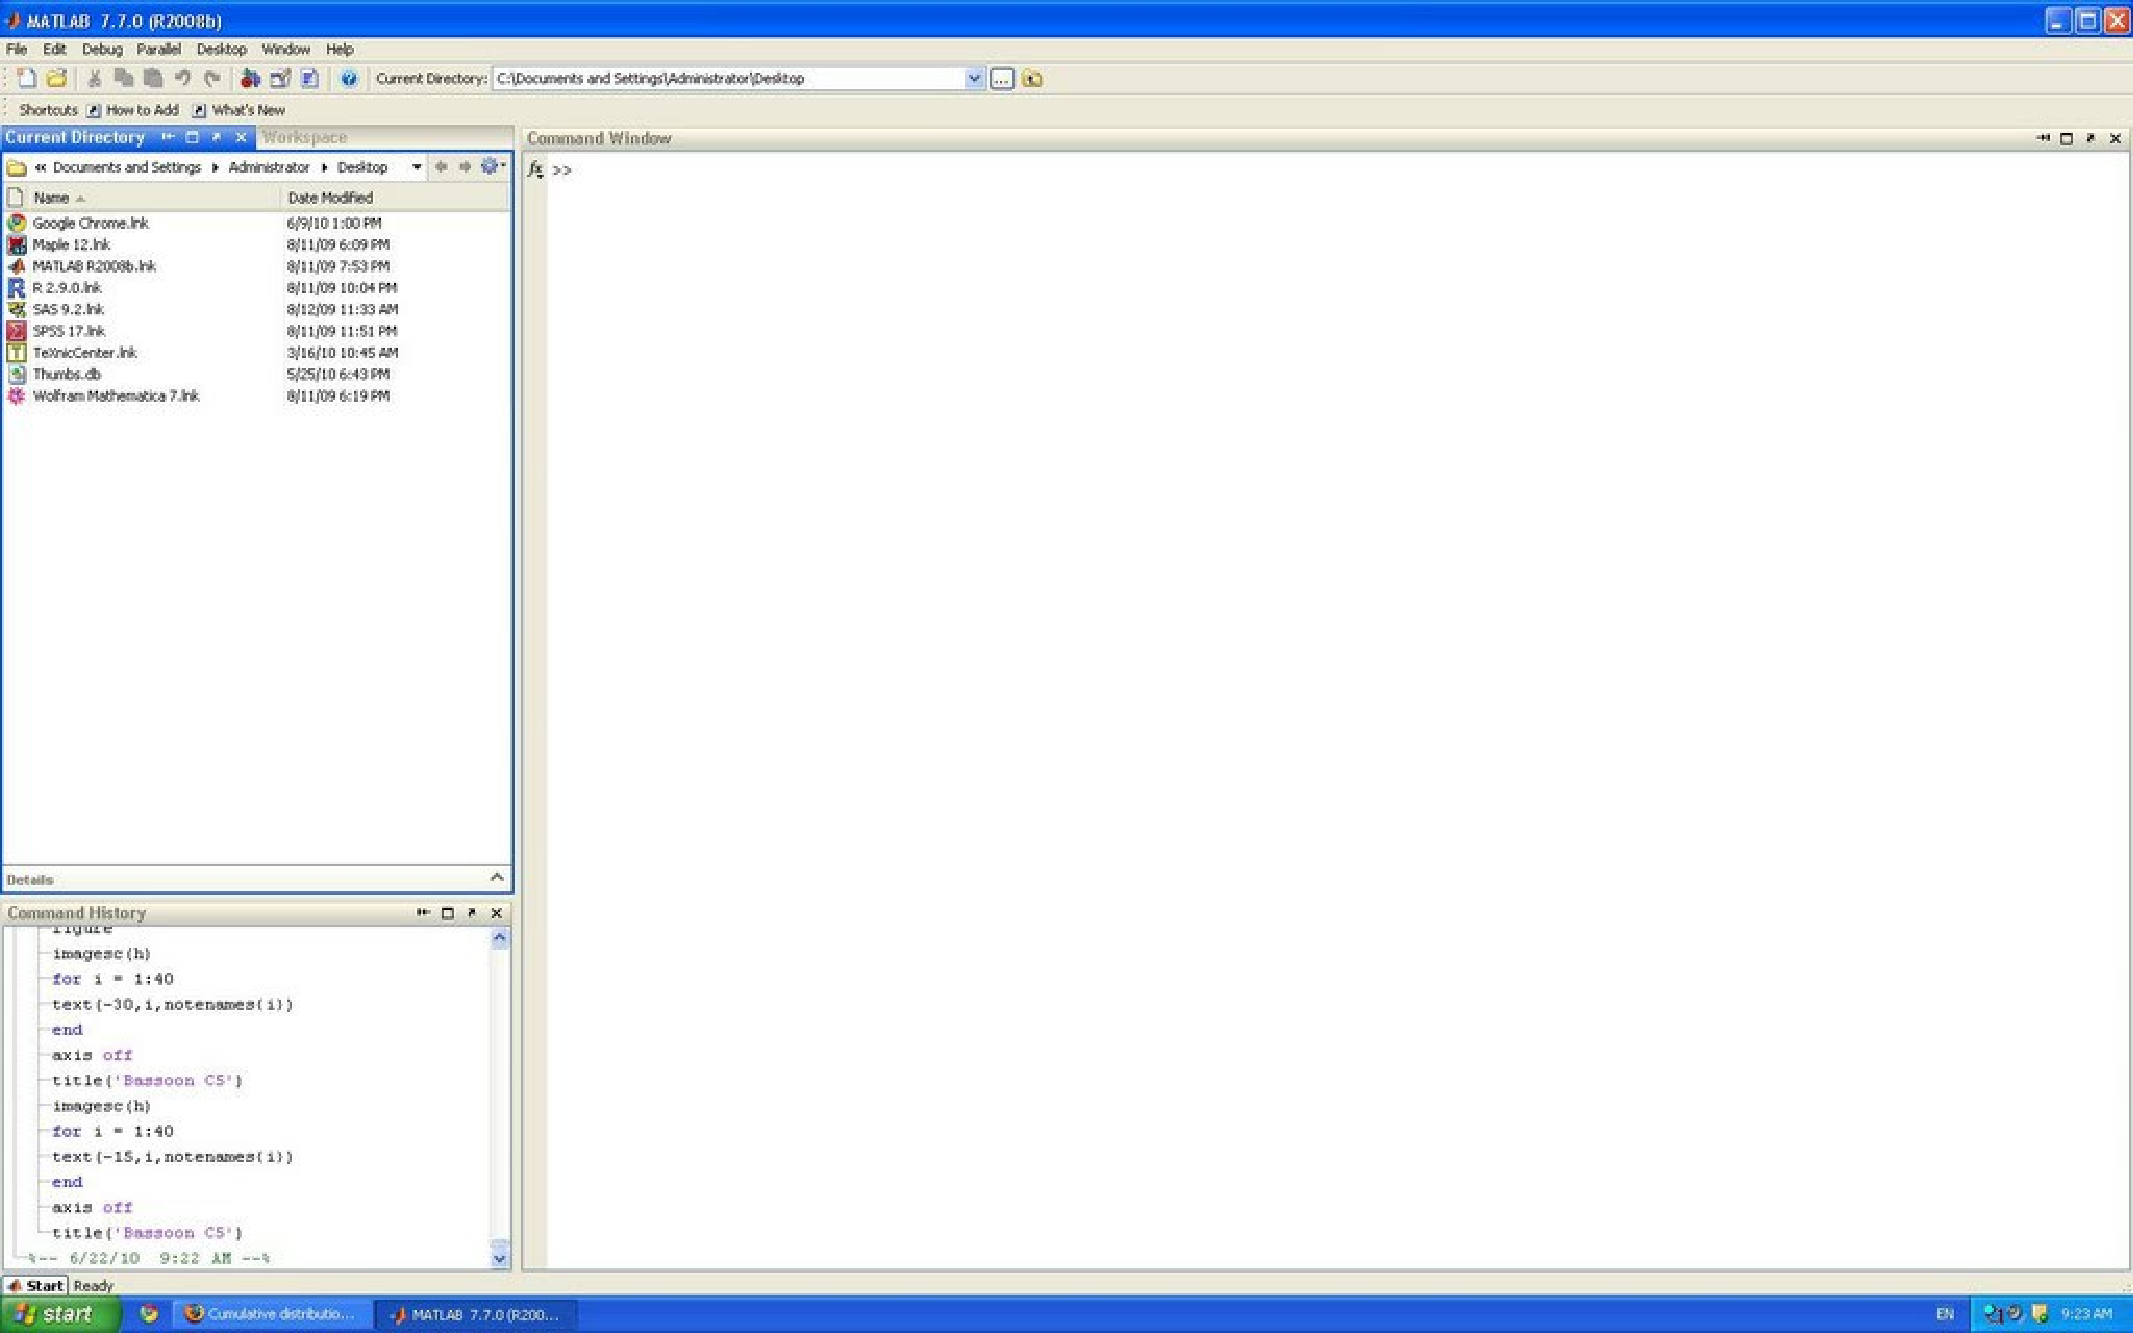
\includegraphics[scale=0.3]{./Figures/homeScreen}
	\caption{The startup screen for MATLAB. The command window is the largest portion of the screen}
\end{center}
\end{figure}


MATLAB is an interpreted language, which means that we can immediately begin executing commands without compiling.  For example, if you type 1 + 1 at the $>>$ prompt in the command window, MATLAB will immediately return the answer. Figure 2 represents basic arithmetic operations we can perform in MATLAB commands:

\begin{figure}[h!]
\begin{center}
	\begin{tabular}{|c|c|}
	\hline
	\li{+} & Addition \\
	\li{-} & Subtraction \\
	\li{*} & Multiplication \\
	\li{/} & Division \\
	\hline
	\end{tabular}
	\caption{Simple Arithmetic Operators}
\end{center}
\end{figure}

\begin{lstlisting}[style=matlab]
>> 1 + 1
ans =
     2
\end{lstlisting}


Now notice the Current Directory panel in figure 1.  Just like a DOS prompt, MATLAB can only see files that are in its current directory and its customizable path.  You can navigate the file structure using the interface in the Current Directory panel, or you may use \li{cd}, \li{dir}, and \li{what} in the command window.  For example:

\begin{lstlisting}[style=matlab]
>> dir
.                            CS312                        ORCA.doc                                    
..                           IMPACT Presentations         ORCA.pdf                       
.DS_Store                    Linearalgebra (1).pdf        PDEs                           
>> cd MATLAB
>> what
M-files in the current directory /Users/jaredwebb/Documents/MATLAB
HelloWorld         coinText           graphscript        outLierRemove      
adjustSet          compareImages      imageReducer       reconSignal        
bigSignal          fourierCompare     littleSignal       sigScript          
coinTest           generateGraphs     myfft              sigTest            
\end{lstlisting}

Note that the \li{what} command lists the m-files in the current directory. M-files are files that contain MATLAB commands.  We discuss M-files in further details in Chapter 1.

\begin{problem}
Create a new text file containing only the string of numbers \li{1 2 3 4 5} and call it \li{data.txt}.  Using the command window, navigate to the location of the file then type \li{load data.txt}.  What happens?
\end{problem}

Also note the Command History and the Workspace panes.  The command history will show all the commands that you have issued in the command window.  You can also access these by using the up or down arrow to cycle through your Command History.  The workspace pane shows all of the current variables that MATLAB is storing.  The \li{who} command will print your workspace to the command line.

\begin{lstlisting}[style=matlab]
>> who
Your variables are:
ans
\end{lstlisting}

\section*{Getting Help}

Even the most experienced MATLAB programmer will run into commands they do not recognize or do not remember how to solve.  In fact, the mark of an experienced programmer is not so much knowing automatically how to use every single MATLAB command as much as it is knowing what resources are available and how to quickly distill those resources into useful commands for the specific problem.

The \li{help} and \li{doc} commands allow you to access the MATLAB documentation about a specific command.  The \li{help} command will give you a detailed plaintext explanation of a command and its parameters, while \li{doc} will bring up details in a browser along with pictures and examples.

When \li{help} and \li{doc} fail there are many resources online that are extremely helpful, especially when dealing with specific problems.  MATLAB is indeed the language of technical computing, and there is an active community of researchers that will have run into and solved myriad problems.  %When in doubt, google.


\begin{center}
\begin{figure}
	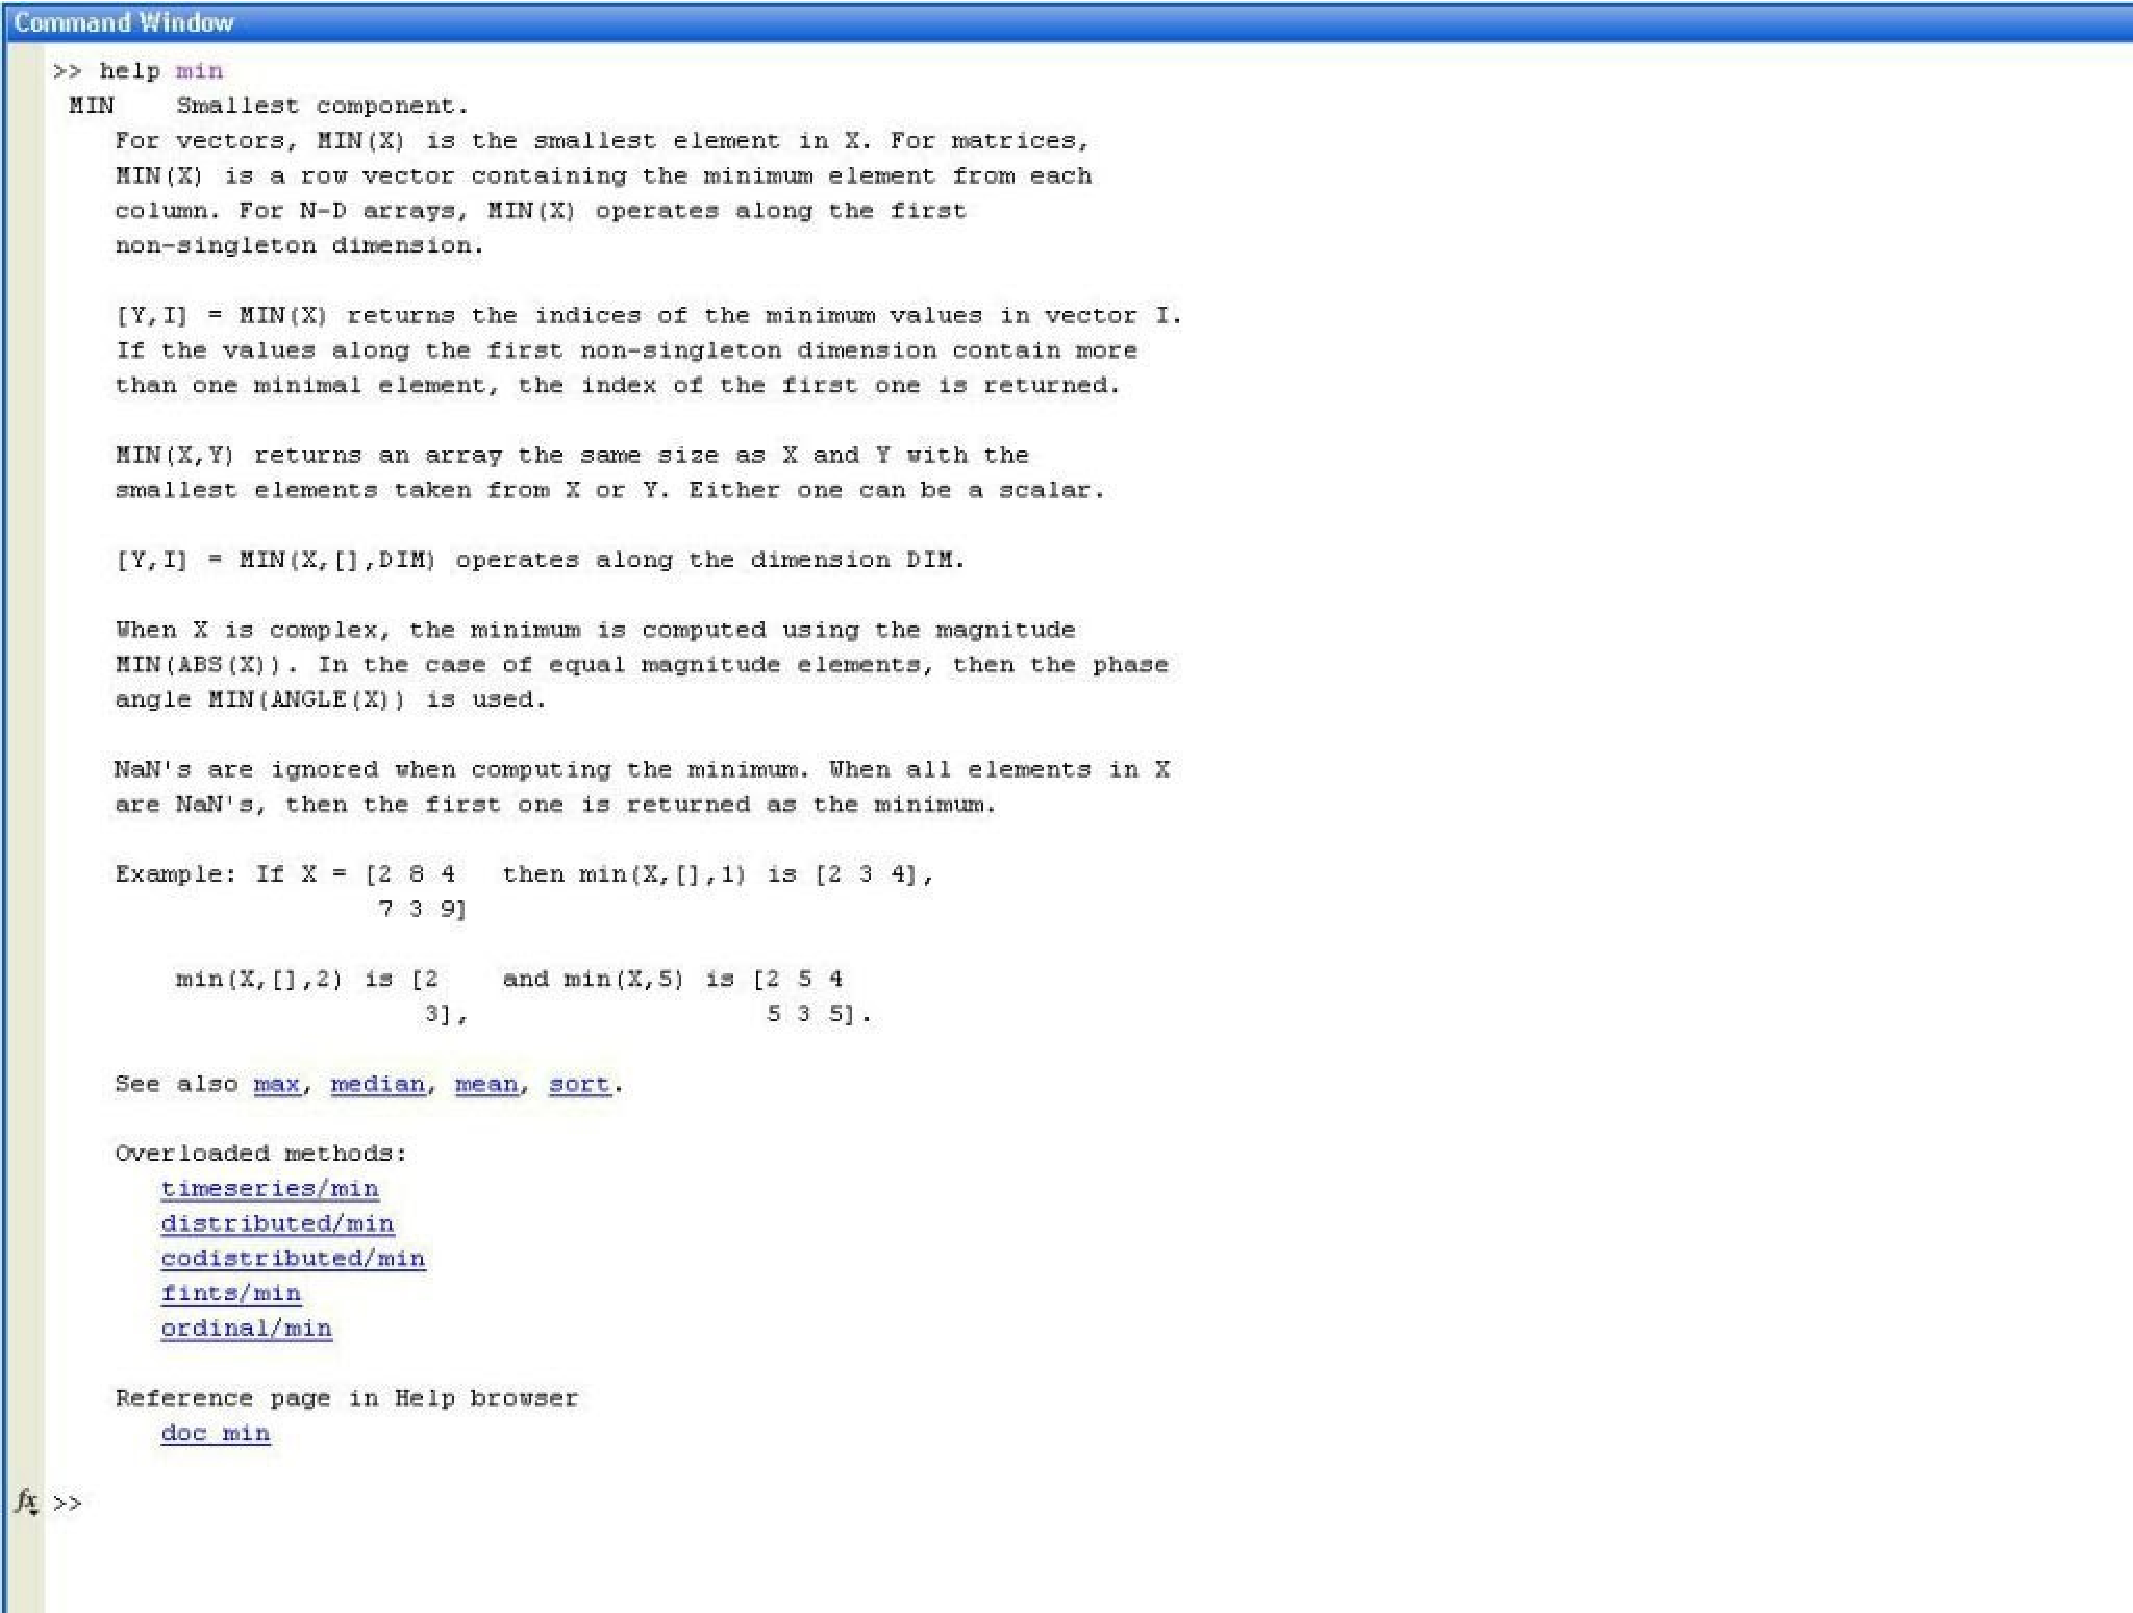
\includegraphics[scale=0.3]{./Figures/help}
	\caption{The help documentation for the \li{min} command. Note that the information displays in the command window.}
\end{figure}
\begin{figure}
	\includegraphics[scale = .3]{./Figures/doc}
	\caption{The documentation window for the \li{min} command. This can be accessed by typing \li{doc min} at the command line.}
\end{figure}
\end{center}

\begin{problem}

Using MATLAB's built in documentation, identify the function of the following commands
\begin{itemize}
	\item fzero
	\item find
	\item linprog
\end{itemize}
\end{problem}

\begin{problem}

Use MATLAB's built in documentation to do the following

\begin{itemize}
	\item Find the zeros of $x^2 - 3x + 2$
	\item Generate a vector of 5 random numbers from a Poisson distribution
	\item Calculate 25 choose 10
\end{itemize}	

\end{problem}

\section*{Setting Variables}

Setting variables in MATLAB happens just as you would expect, using \li{=} to assign a value to a letter or string.

\begin{lstlisting}[style=matlab]
>> x = 3
x =
     3
>> my_variable = 2
my_variable =
     2
>> x + my_variable
ans =
     5
\end{lstlisting}

Placing a semicolon on the end of a MATLAB expression will suppress output.

\begin{lstlisting}[style=matlab]
>> x = 3;
>> my_variable = 2;
>> x + my_variable
ans =
     5
\end{lstlisting}

MATLAB supports several datatypes.  As you become more experienced you will become acquainted with the subtleties of using a specific data type.  We only list them here, noting that in MATLAB the default data type is double.

\begin{figure}[h!]
\begin{center}
	\begin{tabular}{|c|c|}
	\hline
	Class Name & Usage \\
	\hline
	\li{single} & single precision floating point\\
	\hline
	\li{double} & double precision floating point\\
	\hline
	\li{(u)int8} & (un)signed 8 bit integer\\
	\li{(u)int16} & (un)signed 16 bit integer\\
	\li{(u)int32} & (un)signed 32 bit integer\\
	\li{(u)int64} & (un)signed 64 bit integer\\
	\hline
	\li{char} & characters and strings\\
	\hline
	\li{logical} & boolean values\\
	\hline
	\end{tabular}
\end{center}
\caption{Data types in MATLAB}
\end{figure}

\section*{Saving A Workspace}

Large projects can include many variables.  MATLAB allows us to save the entire workspace to a file that can be re-imported.

%Example inserted here%

\begin{figure}
\begin{center}
	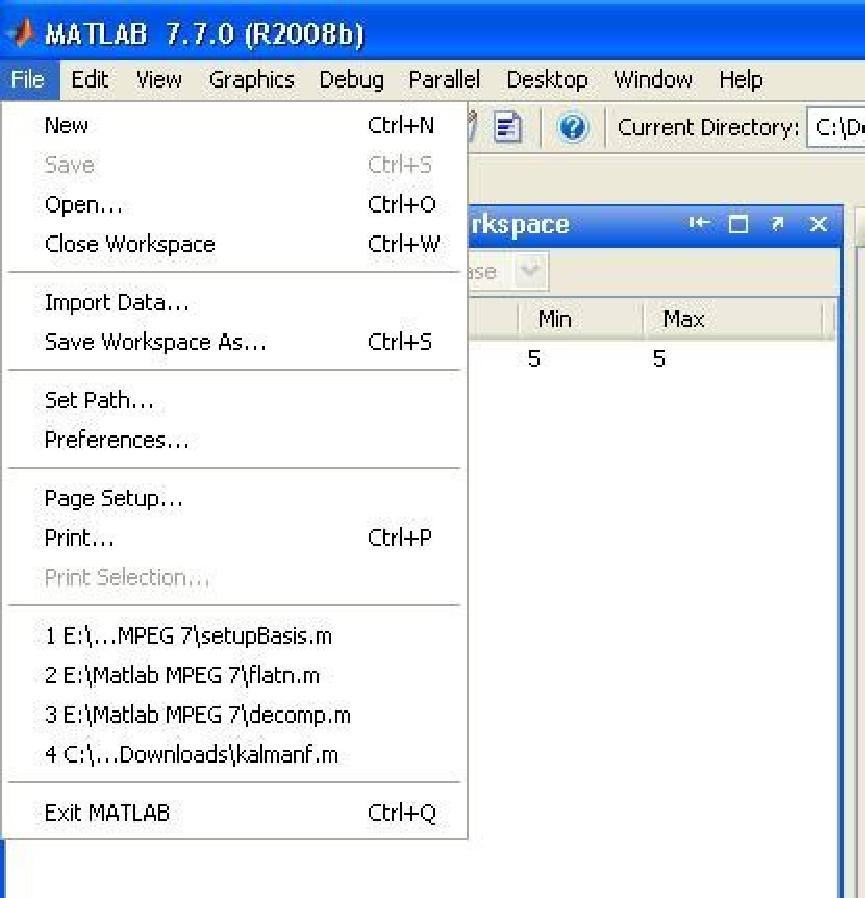
\includegraphics[scale=0.5]{./Figures/saveWorkspace}
	\caption{The file menu. Note the option to save the workspace.}
\end{center}
\end{figure}

\section*{A Note on Floating Point Arithmetic}

In mathematics we expect that the difference between two equal quantities to be zero.  For example, $10 - 10 = 0$.  floating point arithmetic isn't always so precise - altering the previous expression to $e^{log(10)} - 10 = 0$ changes nothing on paper, but try putting it into MATLAB:

\begin{lstlisting}[style=matlab]
>> 10 - 10
ans =
     0
>> exp(log(10)) - 10
ans =
   1.7764e-15
\end{lstlisting}

This is due to floating point arithmetic. Floating point numbers do not have arbitrary precision: they only occupy a certain amount of memory.  For numbers with long decimal expressions or irrational numbers, there will inevitably be a loss of precision because of this memory constraint.  Although these errors will generally be small it is important to understand this limitation of numerical computation. The intricacies of floating point arithmetic will be further developed in Volume II of this work.


\lab{Algorithms}{Matrix Operations and Algorithmic Complexity}{Matrices and Complexity}
\objective{This lesson explains basic matrix operations in MATLAB.}

Matrices form the core data structure in MATLAB. As such we investigate several methods of creating and modifying matrices.

To begin we work with vectors. We demonstrate a variety of methods to create vectors. You should follow these demonstrations on your own computer and experiment as you go. Create a vector using square brackets as follows:

\begin{lstlisting}[style=matlab]
>> b = [1 2 3]
b =
     1     2     3  
\end{lstlisting}

We make a column vector by placing semi-colons between the entries.

\begin{lstlisting}[style=matlab]
>> b = [1;2;3]
b =
     1
     2
     3  
\end{lstlisting}

We combine vectors together by placing two or more of equal dimension inside square brackets. The technical term for this is concatenation.

\begin{lstlisting}[style=matlab]
>> c = [4;5;6]
c =
     4
     5
     6
>> d = [b;c]
d =
     1
     2
     3
     4
     5
     6  
\end{lstlisting}

There are several built-in methods to automate vector creation. For example, we can build a vector of consecutive values using the colon operator, a starting value, and an ending value:

\begin{lstlisting}[style=matlab]
>> 1:5
ans =
     1     2     3     4     5
\end{lstlisting}

This syntax also allows us to specify step size:

\begin{lstlisting}[style=matlab]
>> 1:.5:3
ans =
    1.0000    1.5000    2.0000    2.5000    3.0000
\end{lstlisting}

We can similarly use negative step sizes:

\begin{lstlisting}[style=matlab]
>> 3:-.5:1
ans =
    3.0000    2.5000    2.0000    1.5000    1.0000
\end{lstlisting}

A related function is called \li{linspace}. It allows us to specify two endpoints and the number of equidistant values we want between the two.

\begin{lstlisting}[style=matlab]
>> linspace(1,2,5)
ans =
    1.0000    1.2500    1.5000    1.7500    2.0000
\end{lstlisting}

The \li{plot} function uses two vectors to create a graph, the first vector representing $x$-values and the second representing the corresponding $y$-values.  As an example we plot a line of slope two using the following commands (See Figure \ref{fig:graph}):

\begin{lstlisting}[style=matlab]
>> x = linspace(-2,2,20);
>> plot(x,2*x)
\end{lstlisting}

\begin{figure}
\vspace{-100pt}
\begin{center}
	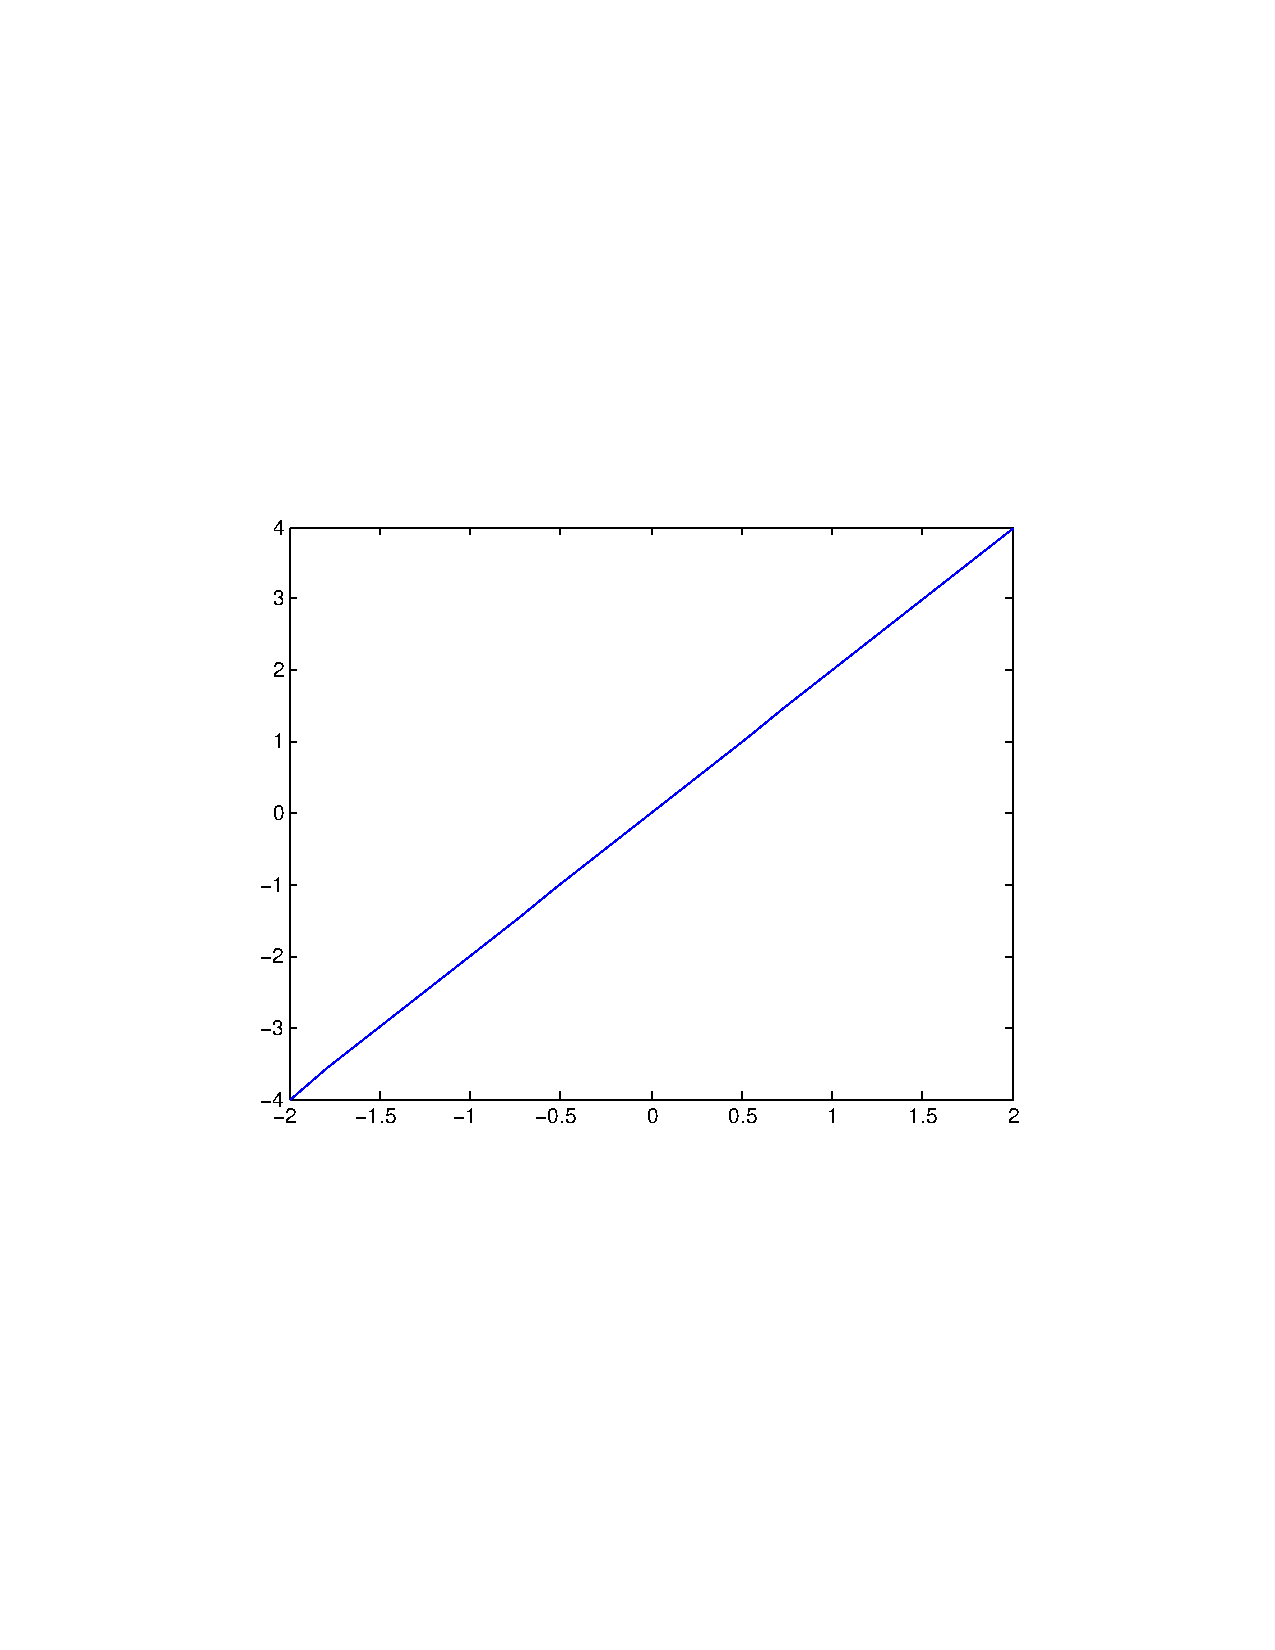
\includegraphics[scale=.5]{./FiguresMAT/graph}
\end{center}
\vspace{-100pt}
\caption{A simple graph}
\label{fig:graph}
\end{figure}

By typing \li{help plot} into the command line we can find the exact syntax and options for the \li{plot} function. For example we can type \li{plot(x,2*x,'r*')} to plot red star data points instead of a line.

\begin{problem}
Plot a line with slope three with black diamond data points. Plot for the domain $x \in [-5,5]$. 
\end{problem}

Creating matrices in MATLAB is done by concatenating vectors in the correct manner. For example:

\begin{lstlisting}[style=matlab]
>> [[1 2 3];[4 5 6];[7 8 9]]
ans =
     1     2     3
     4     5     6
     7     8     9
\end{lstlisting}

\begin{problem}
Create a matrix showing the times table from 1 to 6. Do not enter each number manually. Instead, create a variable \li{x = 1:6} and let the rows of the matrix be multiples of $x$.
\end{problem}

Another technique for creating matrices is using outer products. An outer product is the method of multiplying two vectors to get a matrix. For example, if we want to make a matrix that is two repeated rows of the vector 1:5 we can do the following:

\begin{lstlisting}[style=matlab]
>> [1;1]*(1:5)
ans =
     1     2     3     4     5
     1     2     3     4     5
\end{lstlisting}

Here we are multiplying a $2 \times 1$ vector and a $1 \times 5$ vector, which yields a $2 \times 5$ matrix. The two rows are identical since the entries of the first vector are all ones.

\begin{problem}
Create the same matrix from problem 2, using outer products this time. This implementation, although perhaps more difficult to conceptualize, makes for much more concise code.
\end{problem}

You can also combine matrices in the same way as vectors, as long as the dimensions match correctly, i.e. the same number of rows or the same number of columns. Try the following:

\begin{lstlisting}[style=matlab]
>> D = [b c]
D =
     1     4
     2     5
     3     6
>> E = [D vander(1:3)]
E =
     1     4     1     1     1
     2     5     4     2     1
     3     6     9     3     1  
\end{lstlisting}

Here we used the command \li{vander}, which accepts a vector of length $n$ and creates an $n \times n$ matrix. The columns of this matrix are powers of the input vector (evaluated point-wise). More information about the \li{vander} command can be found by using \li{help}. %We can find more information by typing {\tt help vander}.

To briefly review, vectors are built using the square brackets, with semi-colons to build columns and spaces to build rows. Matrices are built in exactly the same way, using vectors or matrices instead of individual numbers.

Often while writing code for MATLAB it is necessary to know the size of a given matrix. This can be done using the \li{size} or \li{length} function.

\begin{lstlisting}[style=matlab]
>> size(E)
ans =
     3     5
>> length(b)
ans =
     3
\end{lstlisting}

When the input of the \li{length} function is a matrix the function outputs the length of the largest dimension of the matrix.% We can find this information by typing {\tt help length}.

\begin{problem}
The command \li{bucky} generates a matrix that represents the connections between the vertices of a truncated isocahedron. This structure matches both the structure of a standard soccer ball, and also of certain types of carbon molecules known as fullerenes (specifically $C_{60}$, shown in Figure 1.2). It is also related to the structure of the geodesic dome. Find the size of this matrix.
\end{problem}

\begin{figure}[h!]
\begin{center}
\includegraphics[scale = .2]{./Figures/C60a.png}
\caption{The structure of the $C_{60}$ molecule.}
\end{center}
\end{figure}


To access information in a vector or matrix you put the index you wish to access inside parentheses after the variable name. This works for both variable assignment and retrieval.

\begin{lstlisting}[style=matlab]
>> E(2,2)
ans =
     5
>> b(2)
ans =
     2
>> E(2,2) = 3
E =
     1     4     1     1     1
     2     3     4     2     1
     3     6     9     3     1  
\end{lstlisting}

The colon operator is used to retrieve an entire row or column from a matrix.  For example, enter the following to get the second column of a matrix:

\begin{lstlisting}[style=matlab]
>> E(:,2)
ans =
     4
     3
     6
\end{lstlisting}

We similarly retrieve the first row:

\begin{lstlisting}[style=matlab]
>> E(1,:)
ans =
     1     4     1     1     1
\end{lstlisting}

It is also possible to retrieve multiple columns or rows at once. For example, we retrieve the first and third columns of a matrix by entering:
\begin{lstlisting}[style=matlab]
>> E(:,[1 3])
ans =
     1     1
     2     4
     3     9
\end{lstlisting}

We list the entries of a matrix as a vector using the colon operator in the following way:

\begin{lstlisting}[style=matlab]
>> D(:)
ans =
     1
     2
     3
     4
     5
     6
\end{lstlisting}

Essentially, the colon operator tells MATLAB to return all valid entries in that dimension.

There is also a special keyword \li{end} that simply goes to the end of a matrix. The following line tells MATLAB to retrieve the entries in the second row, from the second column to the end:

\begin{lstlisting}[style=matlab]
>> E(2,2:end)
ans =
     3     4     2     1
\end{lstlisting}

Deleting a row or column can be done by assigning an empty matrix ([ ]) to it. For example:

\begin{lstlisting}[style=matlab]
>> E(:,2) = []
E =
     1     1     1     1
     2     4     2     1
     3     9     3     1
\end{lstlisting}
 
\begin{problem}
Try to assign a vector of incorrect size to a piece of a matrix. What happens? Also, try to concatenate two matrices that don't have matching dimensions. What error message do you get? It is important to learn how to read error messages for troubleshooting purposes.
\end{problem}

Basic matrix operations use the characters \li{+}, \li{-} and \li{*}. The transpose (or more precisely the adjoint) can be created by using an \li{'}. Also the \li{^} operator can be used to raise square matrices to a specific power.
\begin{lstlisting}[style=matlab]
>> b+c
ans =
     5
     7
     9
>> b-c
ans =
    -3
    -3
    -3
>> E*[1:4]'
ans =
    10
    20
    34
\end{lstlisting}

Operators can also act element-wise on a matrix by using a period. Experiment with the following:

\begin{lstlisting}[style=matlab]
>> b.*c
ans =
     4
    10
    18
>> b.^c
ans =
     1
    32
   729
>> b./c
ans =
    0.2500
    0.4000
    0.5000
\end{lstlisting}

The majority of elementary functions, such as \li{sin}, \li{cos} and \li{exp} act element-wise on matrices. For example:
\begin{lstlisting}[style=matlab]
>> sin([0:4]*pi/4)
ans =
         0    0.7071    1.0000    0.7071    0.0000    
\end{lstlisting}

There are a variety of functions that let us summarize information about a given matrix. For example, the \li{sum} function returns the sum of each column of a matrix:
\begin{lstlisting}[style=matlab]
>> sum(E)
ans =
     6    14     6     3
\end{lstlisting}

We can also specify the dimension that we want to sum across in our function call. For example, if instead we want to sum across rows we can write:

\begin{lstlisting}[style=matlab]
>> sum(E,2)
ans =
     4
     9
    16
\end{lstlisting}

Some other functions that summarize information about the entries of a matrix are contained in the Table \ref{tbl:summarizefuncs}. Note that each of these functions reduces the size of the matrix (which makes sense, since they are summarizing functions). These functions work across columns by default, although most of them allow you to specify a dimension to work across.

\begin{table}[h!]
\begin{center}
	\begin{tabular}{|c|c|}

    \hline

    Function & Usage \\

    \hline

    \li{max} & Returns maximum entries\\

    \li{min} & Returns mimimum entries\\

    \li{mean} & Returns the mean\\

    \li{median} & Returns the median\\

    \li{std} & Returns the standard deviation\\

    \li{diff} & Returns the differences between entries\\
    
    \li{prod} & Returns the product of entries\\
    
    \li{any} & Returns 1 if there are non-zero entries, zero otherwise\\
    
    \li{all} & Returns 1 if all entries are non-zero, zero otherwise\\

    \li{find} & Returns indices of non-zero entries\\

    \li{norm} & Returns the norm \\ 

    \hline

    \end{tabular}
\end{center}
\caption{Various summarizing functions}
\label{tbl:summarizefuncs}
\end{table}

These functions can be incredibly useful. For example, suppose that we want to estimate the derivative of $sin(x^2)$. A simple approximation for a derivative is
\[
f'(x) \approx \frac{f(x+h) - f(x)}{h}
\]

Presumably this approximation is good when $h$ is small. We use the \li{diff} function to perform this approximation using the following code:

\begin{lstlisting}[style=matlab]
>> h = .001;
>> x = 0:h:pi;
>> approx = diff(sin(x.^2))/h;
\end{lstlisting}

%More awkward wording.  Edit.
Here we evaluate the function $\sin{x}$ at several thousand points between $0$ and $\pi$.  Then, using the derivative estimation formula above, we calculate an approximation of the derivative at each point.  These results are stored in vector \li{approx}.  The analytic solution is:
%What we have done here is evaluate our function at a variety of points close together. We then use the difference of these points to calculate an approximation of the derivative. We have stored these values in the vector {\tt approx}. The actual derivative of this function, calculated by hand is:
\[
f'(x) = 2x cos(x^2)
\]
We write this function (evaluated at the same set of points) as:
\begin{lstlisting}[style=matlab]
>> actual = 2*cos(x.^2).*x;
\end{lstlisting}

%Wording
\begin{problem}
Plot the approximated derivative and the actual derivative on two different plots (the command \li{figure} opens a new plot window, which may be helpful). They should look almost identical. Now use the \li{max} command to find the maximum difference between the estimated derivative and the actual derivative (the dimensions will not match exactly (why?);  fix this by adding or removing an entry from one of the vectors).
\end{problem}

\begin{problem}
The command \li{rand(m,n)} returns a matrix where the entries are ``randomly'' drawn from a uniform distribution between zero and one. Create a vector with ten thousand entries using this command. The theoretical values for the mean($\mu$) and standard deviation($\sigma$) of a uniformly distributed random variable between $a$ and $b$ are
\begin{align*}
\mu &= \frac{a+b}{2} \\
\sigma &= \frac{b-a}{\sqrt{12}}
\end{align*}
These values are calculated using moment-generating functions. Use the functions \li{mean} and \li{std} on the vector you created earlier. How do these compare to the theoretical values?
\end{problem}

The canonical problem in linear algebra is solving the equation $Ax = b$ for x, where $A$ is an $n \times n$ matrix and $b$ is a  $1 \times n$ vector. In linear algebra you probably learned to solve this equation by calculating the matrix inverse. MATLAB calculates the inverse of a matrix using the command \li{inv}. For example, we create a random system $Ax =b$ and solve it using the \li{inv} function (you may check the caclucations by hand):

%Excellent demonstration but needs a bit of work
\begin{lstlisting}[style=matlab]
>> A = [1 3 3; 1 4 3; 1 3 4]
A =
   1   3   3
   1   4   3
   1   3   4
>> b = [3; 7; 1]
b =
   3
   7
   1
>> sol = inv(A)*b
sol =
  -3
   4
  -2
\end{lstlisting}

Recall that a norm is a measurement on the size of a vector.  For example, the Euclidean norm measures the straight line distance from the origin to the ``end'' of a vector.

\[
\norm{x} = \sqrt{x_1^2 + ... + x_n^2}
\]

If the norm of the difference of two vectors is close to zero, then they are good approximations of each other.  The \li{norm} function calculates the euclidean norm of an input vector, and thus we use it to verify that our approximation of the derivative is close to the actual derivative:
% We then verify that we have solved the system by comparing {\tt A*sol} and {\tt b} using the {\tt norm} function:

\begin{lstlisting}[style=matlab]
>> norm(b-A*sol)
ans =
   1.7772e-16
\end{lstlisting}

In addition to the \li{inv} function, MATLAB has an optimized, more general way to solve linear systems. This method is accessed using the backslash operator. We use this operator, and compare it to the solution we found using \li{inv} as follows:

\begin{lstlisting}[style=matlab]
>> sol2 = A\b
sol2 =
    2.4025
   -0.9327
    1.1194
>> norm(sol2-sol)
ans =
   4.5776e-16
\end{lstlisting}

We mentioned that the backslash operator is more efficient than using the function \li{inv}, meaning it returns a result faster. Create the following script to compare the efficiency of each method:

\lstinputlisting[style=matlab, style=fromfile]{./Source/Algorithms/solve_sys.m}

The \li{tic} and \li{toc} commands act as a stopwatch, allowing us to record execution time of various operations.

Now run the script. You should notice a significant difference in execution time (you may need to scale $n$ appropriately). This is because directly calculating a matrix inverse is costly, and MATLAB has optimized procedures for solving linear systems without calculating the inverse. Specifically, MATLAB uses the the LU factorization and backwards substitution to solve the linear system without any matrix inversions.

The backslash operator can also be used to solve several systems at once. For example:

\begin{lstlisting}[style=matlab]
>> A\[b c]
ans =
   -4.4458    6.0150
    7.9111   -1.3294
   -6.5331    5.8585
\end{lstlisting}

%Explain scripts
You might now be asking why we would want to do this. We can answer this by investigating the time it takes to solve two systems. Open a new script file and write the following:

\begin{lstlisting}[style=matlab]
n = 3000;
A = rand(n);
b = rand(n,1);
c = rand(n,1);

tic;
A\b;
A\c;
toc

tic;
A\[b c];
toc
\end{lstlisting}

This script creates a random $3000 \times 3000$ matrix, and two random $3000 \times 1$ vectors (you can experiment with different sizes of matrices and vectors). It then solves the two systems of equations twice, once using two backslash commands and the other using only one. Remember that the semi-colons suppress the output in the script.

Now execute this script. You should notice that the first method takes about twice as long as the second method. This is because the backslash method uses the LU decomposition, and in the second method it only has to execute this factorization once. This highlights the importance of understanding the algorithms that MATLAB uses: we can solve problems much faster if we understand what MATLAB is doing.

A number of other important operators that you will need are found in Table \ref{tbl:matrixops}.

\begin{table}[h!]
\begin{center}

    \begin{tabular}{|c|c|}

    \hline

    Function or Operator & Usage \\

    \hline

    \li{inv} & Matrix inverse\\

    \li{rank} & Rank\\

    \li{norm} & Norm (defaults to 2-norm)\\

    \li{expm} & Matrix exponential\\

    \li{det} & Determinant\\

    \li{eig} & Eigenvalue decomposition\\
    
    \li{svd} & Singular value decomposition\\
    
    \li{lu} & LU decomposition\\
    
    \li{qr} & QR factorization\\
    
    \li{chol} & Cholesky factorization\\

    \hline

    \end{tabular}
	\caption{Useful matrix operations}
\label{tbl:matrixops}
\end{center} 
\end{table}

%Explain better
\begin{problem}
The backslash operator can be also used to solve overdetermined systems. This is sometimes called the least squares method. The formula is $(A^TA)^{-1}A^T*b$. Create a script verify numerically that the backslash operator and the least squares formula yield the same result. Hint: Use the \li{norm} function to verify equality, as we did with \li{inv} and backslash.
\end{problem}

\lab{Algorithms}{Building Matrices, Sparse Matrices and Algorithmic Complexity}{Matrices and Complexity, cont.}

\objective{This section explains how to create specific types of large matrices. It also introduces the concept of temporal complexity. Finally, it explores MATLAB's special commands for working with sparse matrices.}

\section*{Temporal Complexity}

%{\bf The next two paragraphs are an alternate description of Big O, designed as a more intuitive approach, to help with Vol I (a more technical explanation would be in Vol II). Let me know what you think...}

%I am not sure that this is clear or precise enough.  I think that the previously written stuff with some easier problems may be better...

One of the most important questions in Scientific Computing is: How long will this operation take? For this reason we often discuss algorithms in terms of their temporal complexity, which describes how long an operation takes in terms of the size of the input. For example, suppose calculating the inverse of a matrix of size $n$ requires the following number of calculations:
\[
f(n) = \frac{3n^3}{2} + 75n^2 + 250n + 30
\]
What is the most important part of this expression? When our input gets very large the only relevant term in this equation is $n^3$. For this reason we say that $f(n) \in O(n^3)$, or more commonly that $f(n)$ is $O(n^3)$ (spoken ``Big O of n cubed''). This notation is borrowed from analysis. This notation captures the salient behavior of our temporal complexity, or more precisely the growth rate we can expect of the execution time of our algorithm. We discuss this concept further in Lab 1.5, but this is a simple introduction to the notion of complexity and Big O. Spatial complexity is the amount of memory an algorithm uses, and is defined similarly. 

\begin{comment}

Now that we have begun to study some more complex MATLAB expressions, it is prudent to have a basic notion of the complexity of the operations we are interested in executing.  Complexity theory is the study of the difficulty of computational problems.  What makes computing the sum of two integers easy, and what makes computing the inverse of a large matrix so difficult?  There is an entire field dedicated to answering such questions; in this work we only do a cursory examination to communicate the basic ideas and vocabulary.
	
	To begin, we use an example to illustrate what we are trying to accomplish.  There are occasions when one is willing to sacrifice precision in order to focus on more important features of the object of study.  For example, $f(x) = x^3 + \frac{sin(20x)}{10}$ produces a cubic function with a slight wobble.  In some applications that wobble may be a crucial detail, but in many cases the wobble will be irrelevant and only serves to distract from the salient features of the function.  We extend this example to algorithms.

	An algorithm is an ordered set of instructions.  Something simple like a recipe to bake a cake is an algorithm, but the only algorithms you will be dealing with here are MATLAB operations and programs.  To describe the complexity of an algorithm we use asymptotic notation called ``Big O.''  Big O makes us focus on salient features of the complexity of an algorithm while at the same time suppressing unnecessary details, much like we ignored the sine wobble in the previous example.  It has been said that using Big O is ``the art of knowing where to be sloppy and where to be precise.''
	
	With that introduction, we define Big O:
	
\begin{theorem}
	$f(x) = O(g(x))$ if and only if $\exists$ M $\in \mathbb{N}, x_0 \in dom(f)$ such that $|f(x)| \le M|g(x)|$ $\forall x > x_0$
 \end{theorem}
 
 This is an abuse of notation, we really should be saying that $f(x) \in O(g(x))$ since $O(g(x))$ is not a function but an equivalence class of functions.  Lamentably, using $=$ has become embedded into the culture, so there is not much to be done except make a note of the correct notation and move along.
 
 \begin{example}
 $x^2 = O(x^3)$ since $x^2 < x^3$ when $x > 1$
 \end{example}
 
 \begin{example}
 $x^3 + 3x^2 + x + 4 = O(x^3)$ since $x^3 + 3x^2 + x + 4 < 10x^3$ when $x > 1$
 \end{example}
 
  \begin{example}
 $x^2 + 10000x = O(x^2)$ since $x^2 + 10000x < 100000x^2$ for all x.
 \end{example}
 
You can see that when we talk about Big O of polynomials, we are simply dropping off lower order terms and ignoring coefficients.
% 
% (These problems may be too challenging)
% \begin{problem}
% Show that $O(\log{x}) \subset O(x) \subset O(x\log{x})$
% \end{problem}
% 
% \begin{problem}
% Show that $O(x^k) \subset O(x^{k+1})$
% \end{problem}
% 
% \begin{problem}
% Show that $O(x^p) \subset O(2^x)$ for all $p \in \mathbb{N}$
% \end{problem}
% 
	What does this have to do with computer programs?  Every algorithm executed on a computer corresponds to a function that returns the number of steps taken (and therefore the time) given an input of size n.  Certain problems can be solved with fewer steps, whilst others require many more.  For example, given two matrices of size n, it only takes about n steps to add the entries together and thus matrix addition is $O(n)$.  On the other hand, given a matrix of size $n$, it takes about $n^3$ steps to calculate its inverse, and thus inverting a matrix is $O(n^3)$.  There is something inherently more difficult about inverting a matrix; there is complexity that simply isn't there with the straightforward operation of addition.
%	
%	We will return to complexity analysis after we know a little bit more about writing our own scripts and functions.
\end{comment}	
	
\section*{Advanced Matrix Tools}

We now introduce a few different ways to build matrices. Two important commands in building matrices are \li{zeros} and \li{ones}. These commands allow us to build matrices populated with zeros or ones, respectively. For example, to build a 3-vector filled with zeros we enter the following command:

\begin{lstlisting}[style=matlab]
>> zeros(3,1)
ans =
     0
     0
     0
\end{lstlisting}

To find additional options for these commands use the \li{help} command.

%Better explanation and an example or two should go here.

One important use of the command \li{zeros} is to allow us to pre-allocate memory. Pre-allocation is simply the practice of telling MATLAB how large a matrix is going to be when we initialize it. We can always add more space to a matrix using the methods we learned in lab 1, but this requires MATLAB to conduct extra operations internally, because of the way MATLAB allocates computer memory. Thus, it is generally faster to initialize a matrix to its final size and modify its values rather than building a matrix as you go.

%Problem here comparing pre-allocation vs. no pre-allocation.  There should be several orders of magnitude difference.

% Perhaps more of a segue here?

Table 1.3 gives a few commands that allow us to build types of useful matrices.

\begin{table}[h!]

\begin{center}

    \begin{tabular}{|c|c|}

    \hline

    Function & Usage \\

    \hline

    \li{eye} & Identity matrix\\

    \li{zeros} & Zero matrix\\

    \li{ones} & One matrix\\

    \li{diag} & Building (or retrieving) along a diagonal\\

    \li{toeplitz} & Matrix with constant diagonals\\

    \li{triu} & Upper triangular\\
    
    \li{tril} & Lower triangular\\
    
    \li{rand} & Psuedo-random matrix, uniformily distributed\\

   \li{randn} & Psuedo-random matrix, normally distributed\\

   \li{randi} & Psuedo-random matrix, uniformily distributed integers\\
    
    \li{repmat} & Copy across a given dimension\\

    \hline

    \end{tabular}
	\caption{Special matrix creation commands}

\end{center}
\end{table}

For example, suppose that we want to create a matrix with $-2$ on the diagonal, and ones on the super and sub diagonal. We can do this by using the following command:

\begin{lstlisting}[style=matlab]
>> toeplitz([-2,1,0])
ans =
    -2     1     0
     1    -2     1
     0     1    -2
\end{lstlisting}


This matrix is useful because it numerically approximates the second derivative of a function. We investigate some properties of this matrix in Problem 6 of this lab, and explain more about this matrix in Chapter 4.

\begin{problem}
Use the \li{diags} command to create the following matrices. All of these matrices should be easily scaleable (ie only minor modification would be required to change the size).
\[
\begin{pmatrix}
1&2&3&4&5\\
0&1&2&3&4\\
0&0&1&2&3 \\
0&0&0&1&2 \\
0&0&0&0&1 \\
\end{pmatrix}
\hspace{8mm}
\begin{pmatrix}
1&1/2&1/3 & 1/4 &1/5\\
1/2&1&1/2&1/3&1/4\\
1/3&1/2&1&1/2&1/3 \\
1/4&1/3&1/2&1&1/2 \\
1/5&1/4&1/3&1/2&1 \\
\end{pmatrix}
\]

\end{problem}

\begin{problem}
Create the matrices from Problem 1 using the commands \li{toeplitz} and \li{triu}. Which method is easier? Now use whichever command is easiest to create the matrix:
\[
\begin{pmatrix}
1&0&0&0&0\\
0&2&0&0&0\\
0&0&3&0&0 \\
0&0&0&4&0 \\
0&0&0&0&5 \\
\end{pmatrix}
\]
\end{problem}
 
\begin{problem}
Write a script that will create a matrix of size $n$ that has ones on the diagonal and has normally-distributed random entries in the last two columns and the last two rows. Do this in one line using the commands from this section and matrix building techniques from Lab 1.1.
\end{problem}

\section*{Sparse Matrices}

In this section we discuss how sparse matrices are used and constructed. A sparse matrix is a matrix that has few non-zero entries (where few is generally relative to the number of entries in the matrix). Type the following into MATLAB's command window
\begin{lstlisting}[style=matlab]
>> A = diag([2 3 4])
>> B = sparse(A)
>> C = full(B)
\end{lstlisting}
Notice that the matrix $A$ has only three non-zero entries, and so we can consider it sparse. When MATLAB stores a matrix it has to store a floating point number for each entry, meaning that a $3 \times 3$ matrix requires MATLAB to store 9 floating point numbers. However, if we leverage the sparsity of $A$ we realize that we only need to store 3 floating point numbers. The \li{sparse} command does exactly this: it stores a list of non-zero coordinates and their values. In this case MATLAB actually stores the matrix differently, and has a set of optimized operations for sparse matrices. If we want MATLAB to store a matrix that we have designated to be sparse normally we can use the command \li{full}, as we did above.


We remark that if you want to make a sparse diagonal matrix, the
best way to do it isn't to use \li{diag} followed by \li{sparse},
it's actually better to use the \li{spdiags} command:
\begin{lstlisting}[style=matlab]
>> spdiags([2;3;4],0,3,3)
\end{lstlisting}

This is because oftentimes when we are using sparse matrices we are dealing with matrices that are too large to be handled efficiently by MATLAB when represented in full form.

\section*{Banded Matrices}

A banded matrix is one whose only non-zero entries are diagonal
strips.  For example, the matrix
\[
A = \begin{pmatrix} 1&2&0&0\\3&4&5&0\\0&6&7&8\\0&0&9&10
\end{pmatrix}
\]
is banded because there are three nonzero diagonals.  This
particular type of banded matrix is called a tri-diagonal matrix.

You can easily create banded matrices using the \li{diag} command.  For example, the matrix $A$ above can be created by
entering
\begin{lstlisting}[style=matlab]
>> diag([3,6,9],-1) + diag([1 4 7 10],0) + diag([2 5 8],1)
\end{lstlisting}

Often a better way to create a tri-diagonal is it use the \li{spdiags}
command. This is because many diagonal matrices are sparse. For example, we create the same matrix in MATLAB (while designating that it is sparse) using the command:
\begin{lstlisting}[style=matlab]
>> spdiags([3 1 0;6 4 2;9 7 5;0 10 8],-1:1,4,4)
\end{lstlisting}
For more information, check the documentation by typing \li{help spdiags} and/or
\li{doc spdiags}. It can be difficult to visualize a sparse matrix
using the output it produces. For small matrices you can use the \li{full} command to get a better feel for the matrices you are creating. For larger matrices you can use the \li{spy} command. For example we create a tri-diagonal matrix with uniformily distributed random entries.  This will also serve to illustrate the efficiency of sparse matrices.

\begin{lstlisting}[style=matlab]
>> B = rand(1000,3);
>> A = spdiags(B,-1:1,1000,1000);
>> C = full(A);
>> whos("[AC]")
Variables in the current scope:
  Attr Name        Size           Bytes  Class
  ==== ====        ====           =====  ===== 
       A        1000x1000         39980  double %~0.04MB of memory
       C        1000x1000       8000000  double %~7.63MB of memory
\end{lstlisting}

Note that a $2,\!000 \times 2,\!000$ matrix is going to be four times the size of \li{C}.  We can see that the \li{C} will soon grow beyond our ability to represent it in computer memory.  If used the \li{full} command on a matrix of $1,\!000,\!000 \times 1,\!000,\!000$ we will almost immediately bring any standard computer to grinding halt.  This is why sparse matrices are so useful.  They can be used to represent the same data in a fraction of the space. However, we can still visualize this matrix using the \li{spy} command, which essentially shows the location of non-zero entries in a matrix. The output of \li{spy} in this case is shown in Figure 1.2:

\begin{figure}[h!]
\begin{center}
\includegraphics[scale = .5]{./FiguresMAT/spy}
\end{center}
\caption{The output of the \li{spy} command.}
\end{figure}

\section*{Using Sparse Matrices}

Consider the linear system $A x = b$, where $A$ is a
 $100,\!000\times 100,\!000$ tri-diagonal matrix.  To store a full
matrix of that size in your computer, it would normally require 10
billion double-precision floating-point numbers.  Since it takes 8
bytes to store a double, it would take roughly 80GB to store the
full matrix.  For most desktop computers, that fact alone makes the
system numerically prohibitive to solve. The temporal complexity of the problem is even more problematic. Methods for directly solving an arbitrary linear system are usually $O(n^3)$.  As
a result, even if the computer could store an 80GB matrix in RAM, it
would still take several weeks to solve the system.  However, since
we don't have computers with that much available RAM, most of the
matrix would have to be stored on the hard drive, so the computation
would probably take between $6$ months to a year.

The point is that even the next generation of computers will
struggle with solving arbitrary linear systems of this size in a
reasonable period of time.  However, if we take advantage of the
sparse structure of the tri-diagonal matrix, we can solve the linear
system, even with a modest modern computer.  This is because all of
those zeros don't need to be stored and we don't need to do as many
operations to row reduce the tri-diagonal system.

Let's first compute the spatial complexity of the above system when
considered as a sparse matrix.  There are three diagonals that have
roughly $100,\!000$ non-zero entries.  That's $300,\!000$
double-precision floating point numbers, which is about 2.4 MB (Less
storage than your favorite song).  As a result, it will easily
fit into the computer's RAM.  Furthermore, the temporal complexity for solving
a tri-diagonal matrix is $O(n)$. Let's see how long it takes to
solve the system for random data:

\begin{lstlisting}[style=matlab]
>> D = rand(100000,3);
>> b = rand(100000,1);
>> A = spdiags(D,-1:1,100000,100000);
>> tic; A \ b; toc
\end{lstlisting}

\begin{problem}
Write a MATLAB script that returns a full $n\times n$
tri-diagonal matrix with $2$'s along the diagonal and $-1$'s along
the two sub-diagonals above and below the diagonal. Hint: Use the \li{teoplitz} command. Note that this is the second derivative matrix that we discussed at the beginning of this lab.
\end{problem}

\begin{problem}
Repeat the above except have the script return a sparse
matrix. You must build this as a sparse matrix from the beginning. Hint: Use the \li{spdiags} command.
\end{problem}

\begin{problem}
Solve the linear system $A x = b$ where $A$ is the $n\times n$
tri-diagonal matrix from the above two problems and $b$ is randomly
generated.  How high can you go for each method?  Make a table for
several different values of $n$ and the time it took to solve for
each run.  What conclusions can you draw?
\end{problem}

\begin{problem}
Using the sparse matrix above and the command \li{eigs}, calculate the smallest eigenvalue $\lambda$ of the matrix as the matrix's size goes to infinity. What value does $\lambda n^2$ approach (It's the square of an important number)? This is related to operator theory: the second derivative operator has this eigenvalue in certain cases.
\end{problem}

\section*{Other Sparse Commands}

One important command for sparse matrices is the \li{nnz} command, which is related to the number of nonzero entries in a matrix. You can actually pass any matrix into the \li{nnz} function and it returns how many entries are non-zero. When using MATLAB's sparse matrix representation this number is particularly important since it is an indicator of the amount of time and space that is required to operate on the matrix. You should be aware that there is some overhead to using and storing the sparse matrix data structure. Sparsely represented matrices are very beneficial when the number of non-zero entries is relatively small compared to the total number of entries. When the matrix has many non-zero entries, a sparse representation becomes disadvantageous. To see this, create and execute a script with the following code:

\begin{lstlisting}[style=matlab]
A = rand(600); tic; B = A^2; toc
A = sparse(A); tic; B = A^2; toc
\end{lstlisting}
Run the script and note the two different run-times. Notice that it takes about twice as long to perform the operation with the sparse matrix. This is because the sparse matrix data structure is optimized for matrices that are acutally sparse. The matrix $A$ is entirely non-zero. Thus, you incur the overhead of the sparse matrix representation without any benefits since there are no entries you are not required to store or compute. To summarize, only use MATLAB's sparse matrix data structure when your matrices are in fact sparse. Using sparse matrices for mostly full matrices will hurt your performance and memory requirements.

Another important command is the \li{spalloc} command. Sometimes it is necessary to create sparse matrices that do not have a nice banded pattern. To create a general matrix you can operate on, use the \li{spalloc} function. This function takes three arguments: \li{m}, \li{n}, \li{nnzmax}. \li{M} is the number of rows in the matrix, \li{n} is the number of columns, and \li{nnzmax} is the number of nonzero entries you expect the sparse matrix to hold. For example,
\begin{lstlisting}[style=matlab]
A = spalloc(100, 200, 3);
A(1, 34) = 23;
A(23, 32) = 12;
A(99, 109) = 1.23;
\end{lstlisting}
This code snippet creates a $100 \times 200$ sparse matrix with room
for 3 non-zero entries. When the matrix is created all of the entries
are initially assumed to be zero. Notice that we can use the normal
indexing conventions to assign values to these entries. In fact, we
operate on sparse matrices exactly as if they were normal matrices,
except that MATLAB uses special sparse matrix operations to take
advantage of the sparse structure.

The arguments \li{m} and \li{n} in \li{spalloc} are pretty obvious. However,
\li{nnzmax} is a little more subtle. Maybe you don't know exactly how
many nonzero entries you will have; that is OK. When you use {\tt
spalloc} to create a sparse matrix, MATLAB sets aside space for
\li{nnzmax} nonzero entries. When the matrix is created, all of the
entries are assumed to be zero, but the matrix still takes up enough
memory to store \li{nnzmax} entries. If you don't end up using all of
them, the matrix will still operate fast, it will just take up more
space than is needed. What happens if you try to create more
non-zero entries than the \li{nnzmax} value you assigned? This is just
fine as well, except that in this case, MATLAB has to create extra
space for these entries. It is important to note that allocating
space after the matrix is created is time consuming, so you
don't want to do it too often. In general it is probably more
efficient to overestimate the number of entries you will use and
waste a little memory than to do a bunch of allocations because your
NNZMAX value was too small.

For example, type the following script into MATLAB (don't worry if you don't understand all of the syntax, you will very soon):

\begin{lstlisting}[style=matlab]
n = 1e5;
A = spalloc(n,n,n);
B = spalloc(n,n,1);
tic;
for i = 1:n
    A(1,i) = rand(1);
end
toc
tic;
for i = 1:n
    B(1,i) = rand(1);
end
toc
\end{lstlisting}

This script creates two sparse matrices, each $100,\!000 \times 100,\!000$. The difference between the two is that one has pre-allocated $100,\!000$ entries, while the other has only allocated one. We then populate the entries of each matrix the same way, adding a random number one by one. Try running this script. The second method takes significantly longer, and is completely due to pre-allocation.


\lab{Algorithms}{Functions and Logic}{Functions and Logic}

\objective{This section will teach how to build functions. It will also introduce logical statements used in programming.}

Up to this point we have only run scripts. We now introduce a much more powerful and versatile method of problem solving: writing functions.

A function, in the programming sense, is an algorithm that takes in inputs (arguments) and produces outputs. Because of this, the first line of every function that we write will list inputs and outputs in the following manner:

\begin{lstlisting}[style=matlab]
function [out1, out2]=  myfunction(in1,in2)
\end{lstlisting}

The name of the function, in this case, is myfunction. When we write functions we can name them anything we want, and can have as many or as few input arguments as we want. Then, by saving the file in the current MATLAB folder we can call this function at the command line (NOTE: make sure that you name the file the name of the function, otherwise MATLAB may have a hard time finding it).

One important benefit of functions is that any operation done inside a function does not affect variables in the general workspace of MATLAB. This means that we can build complicated functions without worrying about affecting other variables outside of the function. This concept is known as variable scope. When we use variables inside a function they are called ``local variables'', since they do not effect any variables outside of the function.

Let's try an example. Open a new m-file and write the following:

\begin{lstlisting}[style=matlab]
function [x1,x2] = quadrForm(a,b,c)
descr = sqrt(b^2-4*a*c);
x1 = (-b+descr)/2*a;
x2 = (-b-descr)/2*a;
end
\end{lstlisting}

This function takes as inputs the coefficients of a quadratic function and returns the output of the quadratic formula. Save this function as ``quadrForm.m'', and make sure that the current MATLAB directory is where you saved the function. Now at the command line you can use this function.

\begin{lstlisting}[style=matlab]
>> [x1,x2] = quadrForm(1,-2,1)
x1 =
     1
x2 =
     1
\end{lstlisting}

We note that this function is susceptible to floating point error. For example, try to find the roots of the polynomial $x^2 - (10^7 + 10^-7)x + 1$ using our function:

\begin{lstlisting}[style=matlab]
>> [x1 x2] = quadrForm(1,-(1e7 + 1e-7),1)
x1 =
    10000000
x2 =
   9.9652e-08
\end{lstlisting}

Clearly the first root is correct, but the second root is clearly in error (admittedly the error is small, but in this case it is easily fixed). The second root shows the error because it is calculated by subtracting two numbers that are very close together.

We can solve this problem by using slightly different approach. We first calculate the root that is farther from zero using the formula:
\[
x_1 = \frac{-b - \text{sign}(b)*d}{2a}
\]
We can then use a formula known as Viete's formula to calculate the other root:
\[
x_1 x_2 = c/a
\]

\begin{problem}
Write a function that implements this approach. Call it \li{quadrForm2}. Observe the improved performance.
\end{problem}

Most of MATLAB's built-in functions were written in m-files just like the functions you just wrote. Therefore, if you are ever interested in how a built-in function works, you can probably look the actual function up.

%\begin{comment}

\section*{Logic, Conditionals and Loops}


Three basic operators in logic are AND (\li{&&}) OR (\li{||}) and NOT (\li{\~}). We can use relational operators from the Table \ref{tbl:relops} to build logical statements:

\begin{table}[h!]
\begin{center}
\begin{tabular}{|c|c|}
	\hline
	\li{==} & equal to\\
	\li{<} & less than\\
	\li{<=} & less than or equal to\\
	\li{\~} & not equal to\\
	\li{>} & greater than\\
	\li{>=} & greater than or equal to\\
	\hline
\end{tabular}
\caption{Some relational operators}
\label{tbl:relops}
\end{center}
\end{table}

Using these building blocks we can build complicated statements. For example the statement \li{(x>1)&&(x<10)} will return true (1) if $x$ is between one and ten, and false (0) otherwise.

\begin{problem}
Create logical statements for the following:
\begin{enumerate}
\item True if x is prime and less than one-thousand, false otherwise (use the function \li{isprime}).
\item True if $x^2$ is greater than 10 or x is positive and smaller than 2.
\item True if the bessel function of the second kind evaluated at x, with nu = 1, has magnitude greater than 1 (use the function \li{bessely}).
\end{enumerate}
\end{problem}


When we create logical statements based on a vector $x$ we are creating what is known as a bit mask. This bit mask will evaluate to one if the logical statement holds true for that element of $x$, and will be zero if the statement does not hold. Using logical statements as ``masks'' in performing operations is a very powerful tool. For example, suppose we have a vector and we want to add .5 to any number that is less than .5 in that vector. We can do this simply with the following statement:
\[
x = x + .5*(x < .5);
\]

\begin{problem}
Create a function that takes an input vector x and shuffles it like a deck of cards. You may assume that x has even length. The key is to create a mask using some random vector and then assign specific cards to even or odd slots of an output vector using that mask. Remember that you can acess the even entries of a vector using notation like y(2:2:length(x)). Then see how many shuffles it takes to make the output $y$ ``random.'' (you can do this by looking at the offdiagonal entry of corrcoef(x,y), which should be close to zero if the output is random).
\end{problem}


\end{matlab}

%----------------------------------------------------------
%The Elementary Matrices lab is combined into one file

\lab{Algorithms}{Elementary Matrices}{Elementary Matrices}
\label{lab:LUdecomp}
\objective{In this section we will use elementary matrices to find the RREF and to find the LU decomposition.}

In Linear algebra there are 3 elementary row operations: switching two rows, multiplying a row by a constant, and adding a multiple of one row to another row.  We carry out each of these operations with a corresponding elementary matrix.  These matrices are easy to construct. Suppose $A$ is an $m \times n$ matrix and you want to perform one of the three elementary operations on $A$. You can do this be constructing the $m \times m$ identity matrix, $I$, performing the elementary row operation on $I$ to obtain $E$ and then multiplying $EA$.  For example, consider the matrix
\[
A = \begin{pmatrix}
a_{11}&a_{12}&a_{13}&a_{14}\\
a_{21}&a_{22}&a_{23}&a_{24}\\
a_{31}&a_{32}&a_{33}&a_{34}
\end{pmatrix}
\]
If we want to swap the first two rows, we can left multiply the
matrix $A$ by:
\[
E = \begin{pmatrix}
0&1&0\\
1&0&0\\
0&0&1
\end{pmatrix},
\]
then
\[
E A =
\begin{pmatrix}
a_{21}&a_{22}&a_{23}&a_{24}\\
a_{11}&a_{12}&a_{13}&a_{14}\\
a_{31}&a_{32}&a_{33}&a_{34}
\end{pmatrix}.
\]
E in this case is called a type I matrix.
\begin{matlab}
A MATLAB function that creates this elementary matrix is
\begin{lstlisting}[style=matlab]
function out = type1m(n,j,k)
%
% Type I Elementary Matrix
%
out = eye(n); 
out(j,j)=0; 
out(k,k)=0; 
out(k,j)=1; 
out(j,k)=1;
\end{lstlisting}
\end{matlab}

Now let's examine the next row operation.  If we want to multiply,
say, the second row of $A$ by the constant $b$, we can left multiply
the matrix $A$ by the following matrix:
\[
\tilde{E} = \begin{pmatrix}
1&0&0\\
0&b&0\\
0&0&1
\end{pmatrix}.
\]
Then
\[
\tilde{E} A =
\begin{pmatrix}
a_{11}&a_{12}&a_{13}&a_{14}\\
b a_{21}&b a_{22}&b a_{23}&b a_{24}\\
a_{31}&a_{32}&a_{33}&a_{34}
\end{pmatrix}.
\]
$\tilde{E}$ is called a type II matrix.  
\begin{matlab}
The MATLAB code that creates a type II matrix is
\begin{lstlisting}[style=matlab]
function out = type2m(n,j,a)
%
% Type II Elementary Matrix
%
out = eye(n); 
out(j,j)=a;
\end{lstlisting}
\end{matlab}

Now let's examine the last row operation.  If we want to multiply,
say, the first row of $A$ by a constant $c$ and add it to the second
row, we can left multiply the matrix $A$ by the following matrix:
\[
\widehat{E} = \begin{pmatrix}
1&0&0\\
c&1&0\\
0&0&1
\end{pmatrix}.
\]
Then
\[
\widehat{E} A =
\begin{pmatrix}
a_{11}&a_{12}&a_{13}&a_{14}\\
c a_{11} + a_{21}&c a_{12} + a_{22}&c a_{13} + a_{23}&c a_{14} + a_{24}\\
a_{31}&a_{32}&a_{33}&a_{34}
\end{pmatrix}.
\]
$\widehat{E}$ is called a type III matrix.
\begin{matlab}
The MATLAB function that creates this elementary matrix is
\begin{lstlisting}[style=matlab]
function out = type3m(n,j,k,c)
%
% Type III Elementary Matrix
%
out = eye(n); 
out(j,k)=c;
\end{lstlisting}
\end{matlab}

\begin{python}
Below, the elementary matrices corresponding to each row operation is implemented in Python.
\lstinputlisting[style=python, style=fromfile, name=row_opers.py]{./Source/row_opers.py}
\end{python}

\section*{Programming Row Reduction}

A fundamental problem in linear algebra is using matrix representations to solve systems of linear equations.  In this section, we do this by using elementary matrices to reduce a matrix into ``row echelon form'' (REF), as opposed to ``reduced row echelon form'' (RREF).  We remark that to solve a linear system, it is actually faster computationally to use REF and then finish with back-substitution, than it is to use RREF.  Consider the following matrix: 

\[
\begin{pmatrix}
4&5&6&3 \\
2&4&6&4 \\
7&8&0&5
\end{pmatrix}
\]

By iteratively left multiplying by elementary matrices, we can reduce as follows:

\begin{matlab}
\begin{lstlisting}[style=matlab]
>> A = [4 5 6 3; 2 4 6 4; 7 8 0 5]
>> B = type3m(3,2,1,-A(2,1)/A(1,1)) * A
>> C = type3m(3,3,1,-B(3,1)/B(1,1)) * B
>> D = type3m(3,3,2,-C(3,2)/C(2,2)) * C
\end{lstlisting}
\end{matlab}

\begin{python}
Remember that our functions returns the elementary array corresponding to the desired row operation.  Also note that setting the type of our initial array is crucial.
\begin{lstlisting}[style=python]
: import scipy as sp
: import row_opers as op
: A = sp.array([[4, 5, 6, 3],[2, 4, 6, 4],[7, 8, 0, 5]], dtype='float32')
array([[ 4.,  5.,  6.,  3.],
       [ 2.,  4.,  6.,  4.],
       [ 7.,  8.,  0.,  5.]], dtype=float32)
: A1 = sp.dot(op.cmultadd(3,1,0,-A[1,0]/A[0,0]), A); A1
array([[ 4. ,  5. ,  6. ,  3. ],
       [ 0. ,  1.5,  3. ,  2.5],
       [ 7. ,  8. ,  0. ,  5. ]])
: A2 = sp.dot(op.cmultadd(3,2,0,-A1[2,0]/A1[0,0]), A1); A2
array([[  4.  ,   5.  ,   6.  ,   3.  ],
       [  0.  ,   1.5 ,   3.  ,   2.5 ],
       [  0.  ,  -0.75, -10.5 ,  -0.25]])
: A3 = sp.dot(op.cmultadd(3,2,1,-A2[2,1]/A2[1,1]), A2); A3
array([[ 4. ,  5. ,  6. ,  3. ],
       [ 0. ,  1.5,  3. ,  2.5],
       [ 0. ,  0. , -9. ,  1. ]])
\end{lstlisting}
\end{python}

To complete REF we would need to divide each row by its leading
coefficient.  We can do that using Type II matrices.  We leave it to
you to carry this out.

\begin{problem}
\label{prob:REF}
Write a \ProgrammingLanguage function, which takes as input an
$n\times (n+1)$ matrix (in other words and \emph{augmented} matrix) and performs the above naive row reduction to REF using elementary matrices.
\end{problem}

\section*{LU Decomposition}

Again, consider the matrix $A$. By iteratively left multiplying by
elementary matrices, we reduce as follows:

\begin{matlab}
\begin{lstlisting}[style=matlab]
>> A = [4 5 6 3; 2 4 6 4; 7 8 0 5]
>> E1 = type3m(3,2,1,-A(2,1)/A(1,1))
>> B = E1 * A
>> E2 = type3m(3,3,1,-B(3,1)/B(1,1))
>> C = E2 * B
>> E3 =  type3m(3,3,2,-C(3,2)/C(2,2))
>> U = E3 * C
\end{lstlisting}
\end{matlab}

\begin{python}
\begin{lstlisting}[style=python]
: E1 = op.cmultadd(3,1,0,-A[1,0]/A[0,0]); E1
array([[ 1. ,  0. ,  0. ],
       [-0.5,  1. ,  0. ],
       [ 0. ,  0. ,  1. ]])
: B1 = sp.dot(E1, A)
array([[ 4. ,  5. ,  6. ,  3. ],
       [ 0. ,  1.5,  3. ,  2.5],
       [ 7. ,  8. ,  0. ,  5. ]])
: E2 = op.cmultadd(3,2,0,-B1[2,0]/B1[0,0])
: B2 = sp.dot(E2, B1)
: E3 = op.cmultadd(3,2,1,-B2[2,1]/B2[1,1])
: U = sp.dot(E3, B2); U
array([[ 4. ,  5. ,  6. ,  3. ],
       [ 0. ,  1.5,  3. ,  2.5],
       [ 0. ,  0. , -9. ,  1. ]])
\end{lstlisting}
\end{python}
Note that we have reduced the above matrix into upper-triangular
form, denoted as $U$.  Hence, we have
\[
U = E_3 E_2 E_1 A.
\]
Since the elementary matrices are invertible, we also have
\[
(E_3 E_2 E_1)^{-1} U =  A.
\]
This can be re-written as
\[
E_1^{-1} E_2^{-1} E_3^{-1} U =  A.
\]
Then we define $L$ to be
\[
L = E_1^{-1} E_2^{-1} E_3^{-1},
\]
which yields $L U = A$.  
\begin{matlab}
We carry this out in MATLAB:
\begin{lstlisting}[style=matlab]
>> L = inv(E1) * inv(E2) * inv(E3)
>> L * U
\end{lstlisting}
\end{matlab}

\begin{python}
\begin{lstlisting}[style=python]
: from scipy import linalg as la
: I = lambda x: la.inv(x)
: L = sp.dot(sp.dot(I(E1), I(E2)), I(E3)); L
array([[ 1.  ,  0.  ,  0.  ],
       [ 0.5 ,  1.  ,  0.  ],
       [ 1.75, -0.5 ,  1.  ]])
: sp.dot(L, U)
array([[ 4.,  5.,  6.,  3.],
       [ 2.,  4.,  6.,  4.],
       [ 7.,  8.,  0.,  5.]])
\end{lstlisting}
\end{python}
What makes $LU$ decomposition so easy is that the inverses of
elementary matrices are elementary matrices.  For example, the
inverse of a Type 3 elementary matrix is the same matrix with the
opposite sign in the $(j,k)$ entry.  In the above problem, we have:
\begin{matlab}
\begin{lstlisting}[style=matlab]
>> L = type3m(3,2,1,A(2,1)/A(1,1)) * ...
       type3m(3,3,1,B(3,1)/B(1,1)) * ...
       type3m(3,3,2,C(3,2)/C(2,2))
\end{lstlisting}
\end{matlab}
Note that the minus signs are gone.  Doing it this way, we don't
have to actually invert anything to compute $L$.  This makes the
computation much faster.

\section*{Why Should I Care?}

The LU Decomposition isn't very useful when doing matrix computation
by hand.  It is, however, very important in scientific computation
for the following reasons:
\begin{itemize}
\item If you want to solve the matrix equation $A x = b$, for several different $b's$, you can replace $A$ with $L$ and $U$, giving $L U x = b$.  Then solve the equations $L y = b$ and $U x = y$, using forward and backward substitution, respectively.  This is actually faster than solving them with row reduction.
\item The $LU$ decomposition allows quick computation of both inverses and determinants.
\item For very large matrices the $LU$ decomposition is crucial.  Indeed one can perform the $LU$ decomposition on a given matrix $A$ without needing additional space, that is, the program actually over-writes $A$ with $L$ and $U$.  Note that since the diagonal of $L$ are all ones, they don't need to be stored, and so the upper diagonal (including the diagonal) is $U$ and the lower diagonal (not including the diagonal) is $L$.
\end{itemize}

\begin{problem}
\label{prob:LU}
Write a \ProgrammingLanguage function which takes as input
a random $n\times n$ matrix, performs the LU decomposition and
returns $L$ and $U$.  To verify that it works, multiply $L$ and $U$ together
and compare to $A$. Note: you should not use the \li{inv} function when you do this. You should only use the elementary matrices that we just created.
Additionally, have your function count the number of operations needed to perform the LU decomposition.
\end{problem}

\begin{problem}
\label{prob:det}
Write a \ProgrammingLanguage function which uses the solution to Problem \ref{prob:LU} to find the determinant of $A$.
\end{problem}


%-----------------------------------------------------------
%The next few labs are more programming tutorial labs, and are split by language
\begin{python}
\lab{Algorithms}{Conditionals and Loops}{Conditionals and Loops}

\objective{Introduce Loops and Conditionals}

\subsection*{Conditional Statements}
Direct use of relational operators through masking is often the optimal way to do operations. However, there is a more user-friendly way to utilize logical operations.  Introducing the {\tt if} statement.  The {\tt if} statement is often referred to as a branching statement.  Depending on the truth value for the condition, program execution can divirge along many different paths.  The {\tt if} statement in Python is very flexible and powerful.  Consider the following equivalent statements
\begin{lstlisting}
: x if A        #this form is used in python's list comprehensions
: if A: x       #Canonical form (note the colon)
\end{lstlisting}

The {\tt if} statement executes a block of code if a certain condition evaluates {\tt True}.  Below we illustrate the use of an {\tt if} statement to add $1.5$ to an odd number.
\begin{lstlisting}
: a,b = 7,8     #this is called multiple assignment and is valid in python
: if a%2==1:    #% is the modulo operator
....: a += 1.5
: if b%2==1:
....: b += 1.5
: print a,b
\end{lstlisting}

By printing the values we can easily see which if statement executed.  Notice that if the {\tt if} statement evaluated {\tt False}, nothing happened.  There are two things we can do if the initial test condition evaluates {\tt False}.  We can test another condition using an {\tt elif} statement, or we can execute a block a in any case that the first condition is false using an {\tt else} statement.  Let's consider the example above, but with our added syntax.
\begin{lstlisting}
: a,b = 7,8
: if a%2==1:
....: a += 1.5
: elif b%2==1:
: b += 1.5
: else:
....: print "all previous conditions are False"
:
: c,d = 10,11
: if c%2==1:
....: c += 1.5
 else:
....: print "all previous conditions are False"
\end{lstlisting}

Let's look at one more complete example of an {\tt if} statement.  
\begin{lstlisting}
: c = 54
: if c < 30:
....: print "c<30 is True"
: elif c < 40:
....: print "c<40 is True"
: elif c <= 50:
....: print "c<=50 is True"
: else:
....: print "c must be greater than 50"
\end{lstlisting}

\subsection*{Loops}
Loops are another important programming concept. There most general loop is a {\tt while} loop.  A {\tt for} loop is a special case of the {\tt while} loop.

The {\tt while} loop tests a condition, executes a block of code, then tests the condition again.  If the condition is still true, the block of code in the {\tt while} loop is executed again.  This repeats indefinitely or until the condition becomes false.  It is important to \emph{always} ensure that your condition will eventually become false.  If the condition is never false, an \emph{infinite loop} will occur.  A common way to avoid infinite loops is to initialize a counting variable.  If an infinite loop ever does occur, the only way out is to kill the program.  Sometimes the only way to do this is to cut the power to the computer!  Below is an illustration of an infinte while loop (WARNING: don't run this code!)
\begin{lstlisting}
: i = 0 #our counting variable
: while i < 10:
....: print i
....: i -= 1    #decrement our counter
\end{lstlisting}

Notice that the condition never becomes false.  We are waiting until {\tt i} becomes greater than $10$, but {\tt i} is actually decreasing!  It will never reach $10$.

The {\tt for} loop is a while loop with a counter built-in.  The {\tt for} loop is useful for walking through a iteratable objects (lists, tuples, arrays, vectors, etc).  
\begin{lstlisting}
: for i in range(10):
....: print i
0 1 2 3 4 5 6 7 8 9
\end{lstlisting}

The loop will iterate as many times as there are entries in the iterable object. In the for loop example, {\tt i} is called a temporary variable.  Each iteration of the loop, {\tt i} will become be set to the next element in the iterable object.  Python offers a more compact way to write for loops.  It is call \emph{list comprehension}.
\begin{lstlisting}
: [i for i in range(10)]
[0, 1, 2, 3, 4, 5, 6, 7, 8, 9]
: [i+1 for i in range(10) if i%2==1] 
[2, 4, 6, 8, 10]
\end{lstlisting}

List comprehensions always return a list.  It is a more compact and concise  way to write a {\tt for} loop.

Additionally you can document your functions. Python allows you to add a special string at the beginning of each function to describe what the function does.  These are called \emph{docstrings}.
\begin{lstlisting}
: def aFunction(b):
....: """This function takes in an argument b
....: and adds b**2 to it and returns the resutlt"""
....: return b+b**2
: aFunction? # or help(aFunction)
\end{lstlisting}

One last note about loops.  Python has some advanced looping features borrowed from C.  These are {\tt else} clauses, {\tt continue} and {\tt break}.  {\tt while} and {\tt for} loops can have an optional {\tt else} clause.  In {\tt while} loops, the {\tt else} clause is executed when the initial condition is false.  In {\tt for} loops, the {\tt else} clause is executed when the there is no next item in the iterable object.  {\tt continue} skips the rest of the current iteration and continues with the next iteration.  {\tt break} is the opposite of {\tt continue} in that it will break completely out of the current loop.

\begin{problem}
Write a function that will add odd numbers that are less than $n$. While you can use either loop, you will proably find it more convenient to use a {\tt for} loop. Write the solution using list comprehension and the {\tt sum()} function. Compare the runtimes of each solution for $n=10**6$.
\end{problem}

% \begin{problem}
% Now write a second function that does the same thing without using loops (use the {\tt sum} and {\tt find} function). How long does this function take if $n = 10^6$? The first is probably a lot easier to code and understand, but the second runs significantly faster.
% Also, add a help file to your function. Test this out by typing {\tt help myfunctionName}.
% \end{problem}


\begin{problem}
One way to calculate the value of $e^x$ is to use the taylor expansion:
\[
e^x = \sum_{i=0}^\infty{\frac{x^i}{i!}}
\]
This method, however, is problematic when x becomes large (it requires a large number of terms to be accurate). We can utilize what is known as a scaling and squaring method to overcome this problem. This method exploits the property that $e^{2x} = (e^x)^2$. We can thus divide by exponent by two until we get a small enough x to be accurate, and then square the appropriate number of times.
Using while loops and a scaling and squaring method write a function expSS(x) that calculates e(x) using the Taylor Series Expansion. Test your function against {\tt exp()} using $3$ and $30$ as reference values.
\end{problem}

\begin{problem}
Modify the solution of the previous problem to accept an list of inputs and calculate $e^x$ for each input. Make this function as fast as possible by elimating loops when possible (this is called \emph{vectorizing} the function).
\end{problem}
\lab{Algorithms}{Temporal Complexity Revisited}{Temporal Complexity Revisited}

\objective{Learn about the temporal complexity of various matrix operations.}

Now that we have the more sophisticated tools of loops at our disposal, let's take another look at \emph{temporal complexity}. We can estimate empirically the temporal complexity of matrix multiplication. We do this by writing a script to multiply two random square matrices and then we time the operation.
\lstinputlisting[frame=single, name=temporal_complex.py]{./Source/temporal_complex.py}

Note that this script plots the log of the operation and the size of the input (this is what the command \li{plt.loglog()} does). We do this because:
\[
log(x^m) = m log(x)
\]
In this case $x$ is related to the size of our input and $x^m$ is related to the time to solve the problem (essentially we are assuming our operation is in $O(x^m)$). This equation then says that by plotting the log of the input size and computation time will yield a line of slope $m$.
In this case we are calculating the least squares value (using backlash) for the slope, giving a ``best'' estimate of the exponent of the temporal complexity. The value that we get while running this script is about three. This suggests that matrix multiplication is in $O(n^3)$.

Why is this? Let's write our own array multiplication function to figure it out. The following function will multiply two arrays according to the rule of matrix multiplication.
\lstinputlisting[frame=single, name=arrayMult.py, firstline=1, lastline=11]{./Source/arrayMult.py}
 
% \begin{lstlisting}
% function C = MatrMult(A,B)
% [a,b] = size(A);
% [c,d] = size(B);
% C = zeros(a,d);
% for i = 1:a
%     for j = 1:b
%         for k = 1:d
%             C(i,k) = C(i,k) + A(i,j)*B(j,k);
%         end
%     end
% end
% \end{lstlisting}

This is a very simple, naive implementation of array multiplication. Note that there are three nested \li{for} loops. Each loop iterates along one of the array's dimensions. Since they're nested and there's a single ``operation'' at the center you simply multiply the number of iterations in each loop to get the total number of iterations. Unsurprisingly, this is $n^3$.

We note that even though the built-in version of array multiplication has the same temporal complexity as the function you just wrote, they do \emph{not} take the same time to run. You can verify this by running the following:
\begin{lstlisting}
: import scipy as sp
: from timer import timer
: from arrayMult import arrayMult
: A = sp.rand(100,100)
: B = sp.rand(100,100)
: with timer(loop=10) as t:
....: t.time(sp.dot, A, B)
....: t.time(arrayMult, A, B)
....: t.printTimes()
\end{lstlisting}

Why did the two function have significantly different runtimes?  Functions with the same temporal complexity do not take necessarily have the same runtime. It is often possible to improve a function without changing the temporal complexity. One of the primary reasons that we study temporal complexity is to better understand how problems scale.

\begin{problem}
\label{prob:tempcomp1}
Calculate the temporal complexity of the following operations. Use random matrices.
\begin{itemize}
\item Matrix Addition
\item Matrix Inverse
\item Determinant
\item LU decomposition
\item SVD (note that the temporal complexity for this operation is roughly the same as many of these other operations, but that this takes much longer. This again demonstrates that although temporal complexity is incredibly important, it is not the only important factor)
\item Solving a system of equations (remember to use \li{la.solve()}, not \li{la,inv()}).
\end{itemize}
\end{problem}

In Problem \ref{prob:tempcomp1} we calculated the temporal complexity of solving a linear system. \li{la.solve()} is a very efficient way to solve linear systems, however, there are still situations where we can do a better job. For example, suppose that $A$ is generated using the following code:
\begin{lstlisting}
: n = 100
: b = sp.rand(n,1)
: u = sp.rand(n,1)
: v = sp.rand(1,n)
: A = sp.eye(n) + sp.dot(u,v)
\end{lstlisting}

In this case we can use the Sherman-Morrison-Woodbury formula to directly find the inverse quickly:
\[
(A + UCV)^{-1} = A^{-1} - A^{-1}U(C^{-1} + VA^{-1}U)^{-1}VA^{-1}
\]

This formula assumes that $C$ and $A$ are square arrays. In the simple example that we started above $C = 1$. We can solve the system $Ax = b$ using different methods (\li{la.solve()}, \li{la.inv()} and the inversion formula above) and time them using the following code:
\lstinputlisting[name=solvesys.py, frame=single]{./Source/solvesys.py}

\begin{lstlisting}
: import solvesys as ss
: with timer(loops=10) as t:
....: t.time(ss.solveSys, A, b)
....: t.time(ss.invSys, A, b)
....: t.time(ss.smwSys, A, b, n, u, v)
....: t.printTimes()
\end{lstlisting}

We observe that for large $n$, the last method is about four times faster than \li{la.solve()}, and about ten times faster than using \li{la.inv()}. This suggests that at times, special knowledge of a system can be leveraged to greatly improve solution time.

\begin{problem}
Use the Sherman-Morrison-Woodbury formula to solve a system of equation where $A$ is the identity matrix with random entries added to the last column and the last row. Compare performance with \li{la.solve()} and \li{la.inv()}.
\end{problem}

As we have stated several times in this section, algorithms can have the same temporal complexity, but can have quite different runtimes. One method for speeding up looping algorithms is called vectorization. Vectorization is when we replace a loop with a vector operation. This often is slightly harder to code and is more difficult to understand, but it can yield great benefits in terms of computation time. We've already worked with this a little bit, but the array multiplication example is particularly powerful.

When you're taught matrix multiplication typically you're taught to multiply the rows of the first matrix by the columns of the second. In the function we wrote we multiplied each entry individually. Let's replace one of the loops (the \li{j} loop) with an inner product (which is more consistent with how we're taught to multiply matrices anyway). Write a second function for array multiplication that works in this way:
% \begin{lstlisting}
% def MatrMult2(A, B):
%     a,b=A.shape
%     c,d=B.shape
%     C=sp.zeros((a,d))
%     for i in range(a):
%         for j in range(d):
%             C[i,j]=sp.dot(A[i,:], B[:,j])
%     return C
% \end{lstlisting}
\lstinputlisting[frame=single, name=arrayMult.py, firstline=13, lastline=20]{./Source/arrayMult.py}

Now write a script that will compare the run time of the two matrix multiplication functions that you just wrote:
\begin{lstlisting}
from timer import timer
import scipy as sp
from complexity import MatrMult, MatrMult2
n=500
A = sp.rand(n,n)
B = sp.rand(n,n)
C = sp.rand(n,n/2)
with timer() as t:
    t.time(MatrMult, A, B)
    t.time(MatrMult, A, C)
    t.time(MatrMult2, A, B)
    t.time(MatrMult2, A, C)
    t.printTimes()
\end{lstlisting}

We note that the second implementation takes much less time. Recall that this is because MATLAB is optimized to perform vector manipulations. This does not change the asymptotic growth rate of the algorithm (temporal complexity), it simply changes the leading coefficient of that growth rate (which temporal complexity ignores). Clearly by eliminating loops we can often save huge amounts of time.

\end{python}

\begin{matlab}
\lab{Algorithms}{Conditionals and Loops}{Conditionals and Loops}

\objective{Introduce Loops and Conditionals}

Direct use of relational operators through masking is often the optimal way to do operations. However, there is a more user-friendly way to utilize logical operations: \li{if} statements.

An \li{if} statement simply executes a specific operation if a condition holds true. For example, suppose that we want to add one to a number if it is odd. We can do so with the following:

\begin{lstlisting}[style=matlab]
if mod(x,2) == 1
  x = x+1;
\end{lstlisting}

\li{If} statements also have a built-in way to operate if the statement is false. We can do that using the else command.

\begin{lstlisting}[style=matlab]
if mod(x,2) == 1
  x = x+1;
else
  x = x/2;
end
\end{lstlisting}

What does this code do? It adds one to a number if it is odd and divides by two if it is even. Note that the end command is necessary if the ``scope'' of the \li{if} statement spreads more than one line. Also, although the indentation is not required, it is good practice to indent \li{if} statements.

You can also nest \li{if} statemtents. For example:

\begin{lstlisting}[style=matlab]
if x < 5
    x = x+5;
else if x < 10
        x = 10;
    end
end
\end{lstlisting}

This code will add 5 if $x$ is less than 5, and set $x$ to 10 if $x$ is between 5 and 10.

Another statement that can be useful is the \li{switch} statement. It essentially allows us to select from among a number of choices, while a single \li{if} statement only allows us to select one. Here's an example of a switch statement

\begin{lstlisting}[style=matlab]
car = 'camry';

switch car
   case {'camry','corolla'}
      disp('Manufacturer is Toyota')
   case 'mustang'
      disp('Manufacturer is Ford')
   case 'viper'
      disp('Manufacturer is Dodge')
   otherwise
      disp('manufacturer unknown')
end

Manufacturer is Toyota
\end{lstlisting}

These statements are useful if we can pick among several choices (for example if our number is an integer and we need to treat it a number of different ways depending on what it is). These statements, however, are not as useful when we are dealing with decimal numbers.

Loops are another important programming tool. There are two type of loops in MATLAB: \li{for} and \li{while}.

A \li{for} loop is designed to iterate a specified number of times. The syntax is as follows:
\begin{lstlisting}[style=matlab]
for i = vector
   statement
end
\end{lstlisting}

The loop will iterate as many times as there are entries in the vector, with i being equal to a different entry of the vector each time. Suppose we want to add the prime numbers from one to a thousand. We can do so with a \li{for} loop as follows:

\begin{lstlisting}[style=matlab]
x = 0
for i = 1:1000
  if isprime(i)
    x = x+i;
  end
end
\end{lstlisting}

There are two important tools to point out now that you have the power to create meaningful functions. First, in MATLAB files you can add comments anywhere by putting the \% sign. This allows you to explain your code, or remove pieces while testing. This can be done to a complete line (or several lines) by hitting CTRL-R. Lines can be uncommented by using CTRL-T. You should get in the practice of writing comments into your code to explain what you are doing. Also, if you wish to halt whatever MATLAB is working on you can hit CTRL-C.

Additionally you can add help files to your functions. This is done by adding lines of comments directly after the function declaration (the first line of your function). When you type \li{help myFunction} at the command line it will then display however many contiguous comment lines are after the first line of the function.

\begin{problem}
Write a function that adds all of the prime numbers that are less than the input value n. This will simply require copying the code above into a function and modifying it to handle input. How long does it take if $n = 10^6$? 
\end{problem}

\begin{problem}
Now write a second function that does the same thing without using loops (use the \li{sum} and \li{find} function). How long does this function take if $n = 10^6$? The first is probably a lot easier to code and understand, but the second runs significantly faster.
Also, add a help file to your function. Test this out by typing \li{help myfunctionName}.
\end{problem}

The other type of loop is a \li{while} loop. The syntax is:

\begin{lstlisting}[style=matlab]
while condition
  statement
end
\end{lstlisting}

As long as the condition holds true the statement is executed. For example, the following will divide the $x$ by 2 as many times as it takes to make $x$ less than one.

\begin{lstlisting}[style=matlab]
while x > 1
    x = x/2;
end
\end{lstlisting}

\begin{problem}
One way to calculate the value of $e^x$ is to use the taylor expansion:
\[
e^x = \sum_{i=0}^\infty{\frac{x^i}{i!}}
\]
This method, however, is problematic when x becomes large (it requires a large number of terms to be accurate). We can utilize what is known as a scaling and squaring method to overcome this problem. This method exploits the property that $e^{2x} = (e^x)^2$. We can thus divide by exponent by two until we get a small enough x to be accurate, and then square the appropriate number of times.
Using while loops and a scaling and squaring method write a function expSS(x) that calculates e(x) using the Taylor Series Expansion. Test your function against MATLAB's built-in function using values like 3 and 30.
\end{problem}

\begin{problem}
Now modify your function so that it can accept a vector of inputs and calculate $e^x$ for each input. Make this function as fast as possible (investigate eliminating loops, etc).
\end{problem}

One last note about loops is that you can use the \li{break} command to step out of a loop. This can be useful in many cases. For example we could use the \li{break} command in the following code:

\begin{lstlisting}[style=matlab]
for i = 1:10
    x = x/2;
    if x < 1
        break;
    end
end
\end{lstlisting}

This code will divide $x$ by two, up to ten times. If $x$ ever goes below one then MATLAB steps out of the loop.

\lab{Algorithms}{Temporal Complexity Revisited}{Temporal Complexity Revisited}

\objective{Learn about the temporal complexity of various matrix operations.}

Now that we have the more sophisticated tools of loops at our disposal, let's take another look at Temporal Complexity. We can estimate empirically the temporal complexity of matrix multiplication. We do this by writing a script to multiply two random square matrices and then timing the operation.

\begin{lstlisting}[style=matlab]
clear all;
close all;
i = 1500:200:2500;
k = 1;
for n = 1:length(i)
    A = rand(i(n));
    B = rand(i(n));
    tic;
    A*B;
    y(n) = toc;
end
loglog(i,y);
X = [log(i); ones(1,length(i))];
sol = X'\log(y)';
sol(1)
\end{lstlisting}

Note that this script plots the log of the operation and the size of the input (this is what the command \li{loglog} does). We do this because:
\[
log(x^m) = m log(x)
\]
In this case $x$ is related to the size of our input and $x^m$ is related to the time to solve the problem (essentially we are assuming our operation is in $O(x^m)$). This equation then says that by plotting the log of the input size and computation time will yield a line of slope $m$.
In this case we are calculating the least squares value (using backlash) for the slope, giving a ``best'' estimate of the exponent of the temporal complexity. The value that we get while running this script is about three. This suggests that matrix multiplication is in $O(n^3)$.

Why is this? Let's write our own matrix multiplication function to figure it out. Write the following function to multiply matrices:

\begin{lstlisting}[style=matlab]
function C = MatrMult(A,B)
[a,b] = size(A);
[c,d] = size(B);
C = zeros(a,d);
for i = 1:a
    for j = 1:b
        for k = 1:d
            C(i,k) = C(i,k) + A(i,j)*B(j,k);
        end
    end
end
\end{lstlisting}

This is a very simple, naive implementation of matrix multiplication. Note that there are three \li{for} loops. Each loop iterates along one of the matrix dimensions. Since they're nested and there's a single ``operation'' at the center you simply multiply the number of iterations in each loop to get the total number of iterations. Unsurprisingly, this is $n^3$.

We note that even though the built-in version of matrix multiplication has the same temporal complexity as the function you just wrote, they do \emph{not} take the same time to run. You can verify this by running the following:

\begin{lstlisting}[style=matlab]
    A = rand(1000);
    B = rand(1000);
    tic;
    A*B;
    toc;
    tic;
    MatrMult(A,B);
    toc;
\end{lstlisting}

This demonstrates an important principle: functions with the same temporal complexity do not take the same time to run. It is often possible to improve a function without changing the temporal complexity. One of the primary reasons that we study temporal complexity is to better understand how problems scale.


\begin{problem}
Calculate the temporal complexity of the following operations. Use random matrices.
\begin{enumerate}
\item Matrix Addition
\item Matrix Inverse
\item Determinant
\item LU decomposition
\item SVD (note that the temporal complexity for this operation is roughly the same as many of these other operations, but that this takes much longer. This again demonstrates that although temporal complexity is incredibly important, it is not the only important factor)
\item Solving a system of equations (remember to use \li{A\\b}, not \li{inv}).
\end{enumerate}
\end{problem}

In problem 1 we calculated the temporal complexity of solving a linear system. MATLAB's backslash command is very efficient in solving linear systems. However, there are still situations where we can do a better job. For example, suppose that $A$ is generated using the following code:
\begin{lstlisting}[style=matlab]
b = rand(n,1);
u = rand(n,1);
v = rand(1,n);
A = eye(n) + u*v;
\end{lstlisting}

In this case we can use the Sherman-Morrison-Woodbury formula to directly find the inverse quickly:
\[
(A + UCV)^{-1} = A^{-1} - A^{-1}U(C^{-1} + VA^{-1}U)^{-1}VA^{-1}
\]

This formula assumes that $C$ and $A$ are square matrices. In the simple example that we started above $C = 1$. We can solve the system $Ax = b$ using different methods (backslash, \li{inv} and the inversion formula above) and time them using the following code:
\begin{lstlisting}[style=matlab]
tic;
A\b;
toc;

tic;
inv(A)*b;
toc;

tic;
Ainv = eye(n) - eye(n)*u*v/(1+v*u);
Binv*C;
toc;
\end{lstlisting}

We observe that for large $n$, the last method is about four times faster than backslash, and about ten times faster than using \li{inv}. This suggests that at times, special knowledge of a system can be leveraged to greatly improve solution time.

\begin{problem}
Use the Sherman-Morrison-Woodbury formula to solve a system of equation where $A$ is the identity matrix with random entries added to the last column and the last row. Compare performance with backslash and \li{inv}.
\end{problem}


As we have stated several times in this section, algorithms can have the same temporal complexity, but can have quite different run times. One method for speeding up algorithms with loops is called vectorization. Vectorization is when we replace a loop with a vector operation. This often is slightly harder to code and is more difficult to understand, but it can yield great benefits in terms of computation time. This is because MATLAB is optimized to perform vector operations, and so it is usually highly advantageous to give MATLAB commands in that form. We've already worked with this a little bit, but the matrix multiplication example is particularly powerful.

When you're taught matrix multiplication typically you're taught to multiply the rows of the first matrix by the columns of the second. In the function we wrote we multiplied each entry individually. Let's replace one of the loops (the \li{j} loop) with an inner product (which is more consistent with how we're taught to multiply matrices anyway). Write a second function for matrix multiplication that works in this way:
\begin{lstlisting}[style=matlab]
function C = MatrMult2(A,B)
[a,b] = size(A);
[c,d] = size(B);
C = zeros(a,d);
for i = 1:a
    for k = 1:d
        C(i,k) = A(i,:)*B(:,k);
    end
end
\end{lstlisting}

Now write a script that will compare the run time of the two matrix multiplication functions that you just wrote:
\begin{lstlisting}[style=matlab]
n = 500;
A = rand(n);
B = rand(n);
tic;
MatrMult(A,B);
toc;
tic;
MatrMult2(A,B);
toc;
\end{lstlisting}

We note that the second implementation takes much less time. Recall that this is because MATLAB is optimized to perform vector manipulations. This does not change the asymptotic growth rate of the algorithm (temporal complexity), it simply changes the leading coefficient of that growth rate (which temporal complexity ignores). Clearly by eliminating loops we can often save huge amounts of time.

\end{matlab}

%-----------------------------------------------------------
%These labs are primarily Linear Algebra Labs (Factorizations and Applications)
%They are combined

\lab{Algorithms}{QR decomposition}{QR decomposition}

\objective{Understand how the QR algorithm works and write your own implementation.}

The QR decomposition is used to represent any matrix as the multiple of an orthogonal matrix and an upper triangular matrix. This decomposition is useful in computing least squares and is part of a common method for finding eigenvalues.

\section*{Review of Gram Schmidt}

\vspace{5mm}
\begin{theorem}[Gram-Schmidt Orthogonalization Process] Let
$\{\x_i\}_{i=1}^n$ be a basis for the inner product space $V$. Let
\[
\q_1 = \frac{\x_1}{\norm{\x_1}},
\]
and define $\q_2,\q_3,\ldots,\q_n$ recursively by
\[
\q_{k+1} = \frac{\x_{k+1} - \p_k}{\norm{\x_{k+1} - \p_k}},
\]
where
\[
\p_k = \sum^k_{j=1} \langle \x_{k+1}, \q_j\rangle \q_j
\]
is a projection of $\x_{k+1}$ onto the subspace $\mbox{Span}(\q_1,\q_2,\ldots,\q_k)$.  Then the set $\{\q_i\}_{i=1}^n$ is an orthonormal basis for $V$.
\end{theorem}
\vspace{5mm}

For the above algorithm, let $r_{k k} = \|\x_k - \p_{k-1}\|$ and
$r_{j k} = \langle \x_k, \q_j\rangle$.  Then
\begin{align*}
r_{1 1} \q_1 &= \x_1\\
r_{k k} \q_k &= \x_k - r_{1 k} \q_1 - r_{2 k} \q_2 - r_{3 k} \q_3 -
\ldots - r_{k-1, k} \q_{k-1},\quad k=2,\ldots,n.
\end{align*}
This can be written as
\begin{align*}
\x_1 &= r_{1 1} \q_1\\
\x_2 &= r_{1 2} \q_1 + r_{2 2} \q_2\\
\vdots \:\: &= \quad \vdots\\
\x_n &= r_{1 n} \q_1 + r_{2 n} \q_2 + \ldots + r_{n n} \q_{n},
\end{align*}
or in matrix form as
\[
\begin{pmatrix}
\vdots & \vdots & & \vdots\\
\x_1 & \x_2 & \cdots & \x_n\\
\vdots & \vdots & & \vdots
\end{pmatrix}
=
\begin{pmatrix}
\vdots & \vdots & & \vdots\\
\q_1 & \q_2 & \cdots & \q_n\\
\vdots & \vdots & & \vdots
\end{pmatrix}
\begin{pmatrix}
r_{1 1} & r_{1 2} & \cdots & r_{1 n}\\
0 & r_{2 2} & \cdots & r_{2 n}\\
\vdots & \vdots & \ddots & \vdots\\
0 & 0 & \cdots & r_{n n}
\end{pmatrix}.
\]
Hence if our original basis $\{\x_i\}_{i=1}^n$ correspond to column
vectors of a matrix $A$, we can likewise write the resulting
orthonormal basis $\{\q_i\}_{i=1}^n$ as a matrix $Q$ of column
vectors.  Then we have that $A = Q R$, where $R$ is the above
nonsingular upper-triangular $n\times n$ matrix.  This is the QR
Decomposition and is summarized by the following theorem:
\vspace{5mm}
\begin{theorem}
Let $A$ be an $m\times n$ matrix of rank $n$.  Then $A$ can be
factored into a product $Q R$, where $Q$ is an $m\times n$ matrix
with orthonormal columns and $R$ is a nonsingular $n \times n$ upper
triangular matrix.
\end{theorem}

\begin{matlab}
There are several options to MATLAB's QR routine.  We will be using
the ``economy option''.  Type the following into MATLAB
\begin{lstlisting}[style=matlab]
>> A = randn(4,3)
>> [Q,R] = qr(A,0)
>> Q*R
>> Q'*Q
\end{lstlisting}
\end{matlab}

\begin{python}
There are three mode options available in SciPy's implementation of QR Decomposition.  We will be using the ``economic" option.
\begin{lstlisting}[style=python]
: import scipy as sp
: from scipy import linalg as la
: A = sp.randn(4,3)
: Q, R = la.qr(A, mode='economic')
: sp.dot(Q, R) == A     there will be some False entries
: sp.dot(Q, R) - A
: sp.dot(Q.T, Q)
\end{lstlisting}
\end{python}

In order to interpret the results correctly, we need to understand that the computer has limited precision (especially with floating point numbers).  This is why \li{sp.dot(Q, R)} is not exactly equal to A.  But subtracting the two yields numbers that are essentially zero.  This shows that indeed the product of $Q$ and $R$ is $A$.  Note also that $Q^T Q = I$.  This implies that the column vectors of $Q$ are orthonormal (why?).

\section*{Solving Least Squares Problems}

For large or ill-conditioned problems, the QR decomposition provides
a nice method for computing least squares solutions of
over-determined matrices.  Consider the problem $A x = b$.  Recall
that the least squares solution is $\widehat x = (A^T A)^{-1}A^T b$.
Alternatively, we write the linear system as
\[
Q R x = b.
\]
We then multiply both sides by $Q^T$, yielding
\[
R x = Q^T b.
\]
Then $\widehat x = R^{-1} Q^T b$.

\section*{Computational Remark}

Numerically, the Gram Schmidt process can have problems due to
finite precision arithmetic. Specifically, due to rounding errors,
the resulting basis may not be orthonormal. To combat this, we
actually carry out a slightly revised algorithm called Modified Gram
Schmidt.  To do this, we compute $\q_1$ as before.  We then project
it out of each of the remaining original vectors
$\x_2,\x_3,\ldots,\x_n$ via
\[
\x_k := \x_k - \langle \x_{k}, \q_1\rangle \q_1,\quad k=2,\ldots,n.
\]
Then we compute $\q_2$ to be the unit vector of $\x_2$, that is,
\[
\q_2 = \frac{\x_2}{\|\x_2\|}.
\]
We repeat by projecting out $\q_2$ from the remaining vectors
$\x_3,\x_4,\ldots,\x_n$.

\begin{problem}
\label{prob:QR}
Write your own \ProgrammingLanguage function which takes as
input the matrix $A$ and computes its QR decomposition, returning the matrices $Q$ and $R$.  
Be sure to use the numerically stable Modified Gram Schmidt algorithm.
\end{problem}

\lab{Applications}{Linear Algebra in Statistics}{Statistics}
\label{Stats1}

\objective{This section will teach about using \ProgrammingLanguage~to solve problems in statistics. This will include finding means, correlation matrices, and solving least squares problems.}

\section*{Shifting Data by the Mean}

Consider the table below representing students scores in a class.\\

\begin{figure}[h!]
\begin{center}
\begin{tabular}{|c|r|r|r|r|}
	\hline
Student & Homework & Exam 1  & Exam 2 & Final \\
\hline
S1  & 89 & 91 & 77 & 75 \\
S2  & 67 & 72 & 76 & 66 \\
S3  & 72 & 77 & 69 & 70 \\
S4  & 56 & 60 & 55 & 61 \\
S5  & 92 & 98 & 89 & 86 \\
S6  & 83 & 88 & 90 & 84 \\
S7  & 45 & 60 & 55 & 48 \\
\hline
Average  & 72 & 78 & 73 & 70\\
\hline
\end{tabular}\\
\end{center}
\end{figure}

We can shift our data set by subtracting each column by its average value.  This makes it so that the average of each column in the matrix below is zero.  If $W$ represents the matrix of scores, the following \ProgrammingLanguage command will subtract out the average.  Why does this work?
\begin{matlab}
\begin{lstlisting}[style=matlab]
>> X = W - ones(7,1)*mean(W)
\end{lstlisting}
\[
X=
\begin{bmatrix}
17 & 13 & 4 & 5 \\
-5 & -6 & 3 & -4 \\
0 & -1 & -4 & 0 \\
-16 & -18 & -18 & -9 \\
20 & 20 & 16 & 16 \\
11 & 10 & 17 & 14 \\
-27 & -18 & -18 & -22.
\end{bmatrix}
\]
\end{matlab}
\begin{python}
\begin{lstlisting}[style=python]
:X = W - sp.dot(sp.ones((7,1),dtype=sp.float_),sp.mean(W,axis=0).reshape(1,4));X
array([[ 17.,  13.,   4.,   5.],
       [ -5.,  -6.,   3.,  -4.],
       [  0.,  -1.,  -4.,   0.],
       [-16., -18., -18.,  -9.],
       [ 20.,  20.,  16.,  16.],
       [ 11.,  10.,  17.,  14.],
       [-27., -18., -18., -22.]])
\end{lstlisting}
\end{python}

\section*{Angles Between Vectors}

Inner products give information about lengths of vectors and angles between vectors.  Recall that the angle $\theta$ between two vectors is given by
\[
\cos{\theta} = \frac{\ipt{x}{y}}{\norm{x}\norm{y}}
\]
where the norm (or length) of a vector is $\norm{x} = \sqrt{\ipt{x}{x}}$.  Note that the usual inner product in $\mathbb{R}^n$ is given by
\[
\ipt{x}{y} = x^T y
\]
Alternatively, if we can first divide our vectors by their length (these are called unit vectors) and then take the inner product
\[
\cos{\theta} = \left\langle\frac{x}{\norm{x}},\frac{y}{\norm{y}}\right\rangle
\]
Hence, we can find the cosine of the angles between our data columns in $X$ by dividing each column by its length.  There are a couple of ways of doing this.  The following is an interesting way of doing it.  Be sure to explore why it works:
\begin{matlab}
\begin{lstlisting}[style=matlab]
>> Y = X ./ (ones(7,1)*sqrt(diag(X'*X)).')
\end{lstlisting}
\end{matlab}
\begin{python}
\begin{lstlisting}[style=python]
: Y = X / sp.dot(sp.ones((7,1),dtype=sp.float_),sp.sqrt(sp.diag(sp.dot(X.T,X)).T).reshape(1,4));Y
array([[ 0.39848615,  0.35329218,  0.11386819,  0.15371887],
       [-0.11720181, -0.16305793,  0.08540114, -0.12297509],
       [ 0.        , -0.02717632, -0.11386819,  0.        ],
       [-0.37504578, -0.48917378, -0.51240685, -0.27669396],
       [ 0.46880723,  0.54352643,  0.45547275,  0.49190037],
       [ 0.25784398,  0.27176321,  0.4839398 ,  0.43041282],
       [-0.63288976, -0.48917378, -0.51240685, -0.67636301]])
\end{lstlisting}
\end{python}
Hence we have:
\[
Y=
\begin{bmatrix}
0.3985 & 0.3533 & 0.1139 & 0.1537\\
-0.1172 & -0.1631 & 0.0854 & -0.1230\\
0 &-0.0272 &-0.1139 & 0\\
-0.3750 & -0.4892 & -0.5124 & -0.2767\\
0.4688 & 0.5435 & 0.4555 & 0.4919\\
0.2578 & 0.2718 & 0.4839 & 0.4304\\
-0.6329 & -0.4892 & -0.5124 & -0.6764
\end{bmatrix}
\]
Finally, we get the cosines of the angles between columns by computing $Y^T Y$.  In \ProgrammingLanguage, that's just
\begin{matlab}
\begin{lstlisting}[style=matlab]
>> Y'*Y
\end{lstlisting}
\end{matlab}
\begin{python}
\begin{lstlisting}[style=python]
: sp.dot(Y.T,Y)
array([[ 1.        ,  0.97782999,  0.89014869,  0.94908967],
       [ 0.97782999,  1.        ,  0.90978843,  0.92490144],
       [ 0.89014869,  0.90978843,  1.        ,  0.9276955 ],
       [ 0.94908967,  0.92490144,  0.9276955 ,  1.        ]])
\end{lstlisting}
\end{python}
This yields
\[
Y^T Y = 
\begin{bmatrix}
1.0000 & 0.9778 & 0.8901 & 0.9491\\
0.9778 & 1.0000 & 0.9098 & 0.9249\\
0.8901 & 0.9098 & 1.0000 & 0.9277\\
0.9491 & 0.9249 & 0.9277 & 1.0000
\end{bmatrix}.
\]
Note that the $(j,k)$ entry of $Y^T Y$ corresponds to the cosine of the angle between the $j^{th}$ and $k^{th}$ columns.  We remark that the diagonals are always equal to one because the angle between a vector and itself is zero and the cosine of zero is one.

\section*{Correlation}

We remark that the cosine of the angle between two vectors is sometimes called the correlation coefficient.  Two columns are said to be 
\begin{itemize}
\item Perfectly correlated if the cosine of the angle between them is one.
\item Positively correlated if the cosine of the angle between them is between zero and one.
\item Uncorrelated if the cosine of the angle between them is zero.
\item Negatively correlated if the cosine of the angle between them is between negative one and zero.
\item Perfectly anticorrelated if the cosine of the angle between them is negative one.
\end{itemize}

The notion of correlation is important in establishing the relationships between measurements.  For example, there is a high correlation between those who smoke and those who get lung cancer.  It's important to understand that the high correlation alone does not necessarily imply that smoking causes lung cancer, it only links them statistically.  This is the famous issue of causation versus correlation.  For example, there is a high correlation between crime rates and sales of ice cream.  This doesn't mean that ice cream causes crime or that increases in crime makes people want to eat more ice cream, but both rates do go up in the summer.

\begin{problem}
Download the file lab8.txt from the following link:
\url{http://www.math.byu.edu/~jeffh/teaching/m343h/lab8.txt}
You can load this datafile by typing
\begin{matlab}
\li{load lab8.txt}
Note that the data is available in the matrix \li{lab8}.  This consists of two columns.  Find the correlation coefficient of the two columns.  Then plot the original data and see if the value that you got is reasonable.
\end{matlab}
\begin{python}
\li{lab8 = sp.genfromtxt("lab8.txt")}
The data is now available in the array \li{lab8} (also, make sure Python is working in the directory of lab8.txt).  \li{lab8} consists of two columns.  Find the correlation coefficient of the two columns.  Then plot the original data and see if the value that you got is reasonable.
\end{python}
\end{problem}

\section*{Least Squares}

It is well known that the displacement of a spring is proportional to the force acting upon it, that is, $F = k x$.  The proportionality constant $k$ is called Hooke's spring constant.  Consider a laboratory experiment where different loads are placed on a spring and the displacement is measured and recorded in the table below:
\vspace{5mm}\\
\begin{center}
\begin{tabular}{|c|c|}
	\hline
x & F \\
(cm) & (dyne)\\
\hline
1.04  & 3.11 \\
2.03  &  6.01\\
2.95  &  9.07\\
3.92  &  11.99\\
5.06  &  15.02\\
6.00  &  17.91\\
7.07  &  21.12\\
\hline
\end{tabular}
\end{center}
\vspace{5mm}
To find the spring constant $k$, we simply need to solve the following linear system
\[
\begin{pmatrix}
1.04\\
2.03\\
2.95\\
3.92\\
5.06\\
6.00\\
7.07\\
\end{pmatrix}
\begin{pmatrix}k\end{pmatrix} = 
\begin{pmatrix}
3.11 \\
6.01\\
9.07\\
11.99\\
15.02\\
17.91\\
21.12\\
\end{pmatrix}.
\]
However, there is no solution to this system because it is overdetermined.  Instead, we seek the ``best'' $k$ that fits the data.  Least squares (which we mentioned in a previous exercise) allows us to find that ``best'' solution. We can find the least squares solution by computing the following in \ProgrammingLanguage:
\begin{matlab}
\begin{lstlisting}[style=matlab]
>> A = [1.04;2.03;2.95;3.92;5.06;6.00;7.07];
>> b = [3.11;6.01;9.07;11.99;15.02;17.91;21.12];
>> k = inv(A'*A)*A'*b
\end{lstlisting}
\end{matlab}
\begin{python}
\begin{lstlisting}[style=python]
: A = sp.array([[1.04],[2.03],[2.95],[3.92],[5.06],[6.00],[7.07]])
: b = sp.array([[3.11],[6.01],[9.07],[11.99],[15.02],[17.91],[21.12]])
: k = sp.dot(sp.dot(la.inv(sp.dot(A.T,A)),A.T),b);k
array([[ 2.99568294]])
\end{lstlisting}
\end{python}
Hence, we find the spring constant to be $k = 2.9957$.  We plot the data against the best fit as follows:
\begin{figure}[h!]
\label{fig1}
\begin{center}
\begin{matlab}
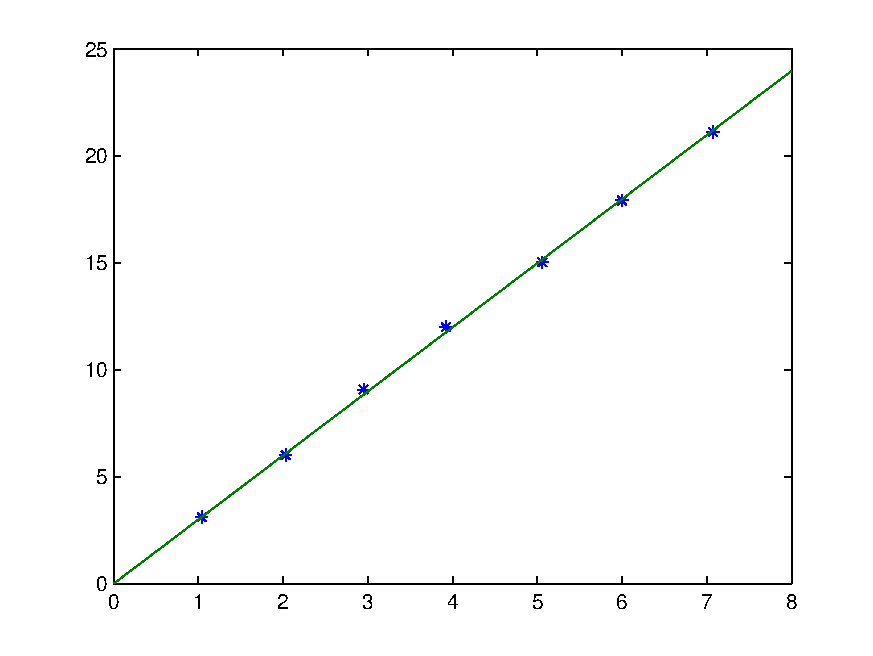
\includegraphics[scale = .6]{./FiguresMAT/lab9_line}
\end{matlab}
\begin{python}
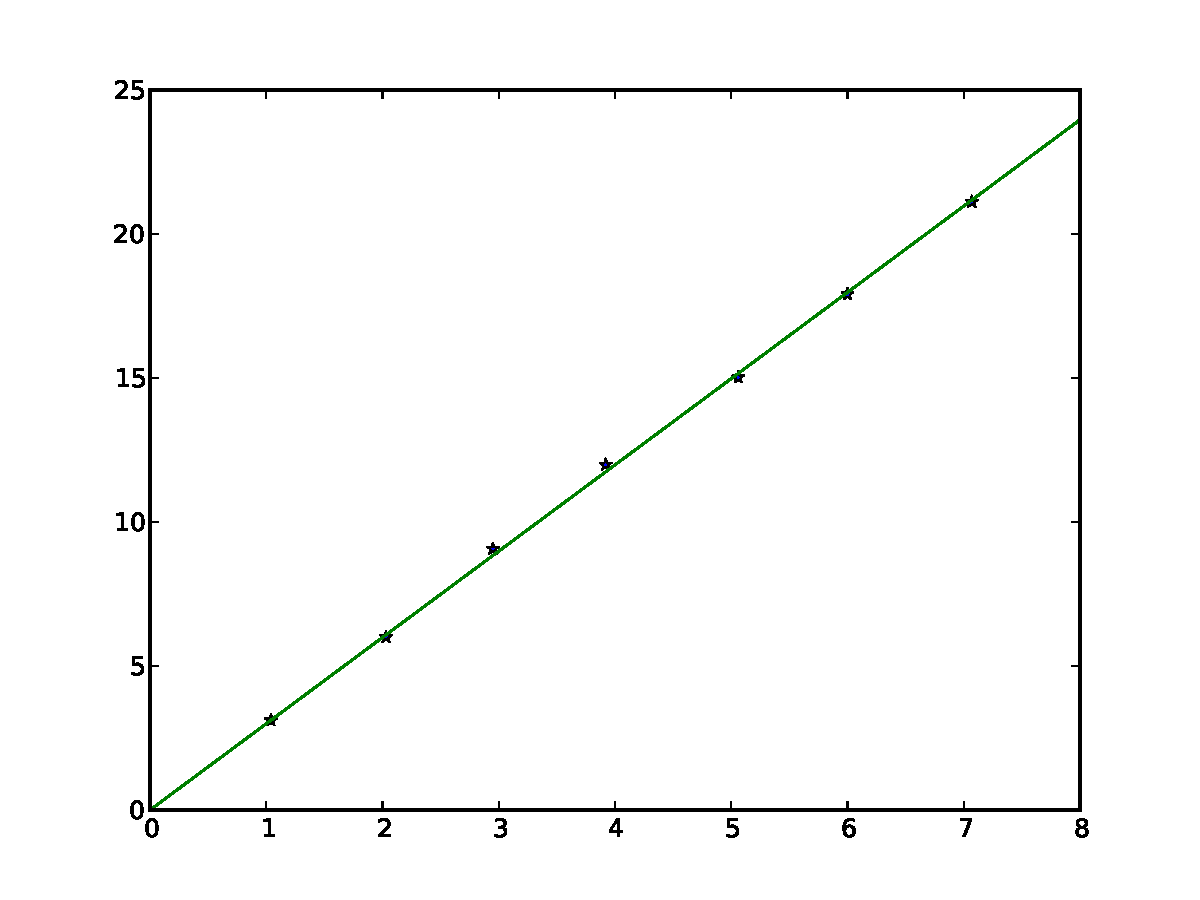
\includegraphics[scale = .6]{./Figures/lab9_line_py}
\end{python}
\caption{The graph of the spring data together with its linear fit}
\label{Fig:SpringFit}
\end{center}
\end{figure}

\begin{matlab}
\begin{lstlisting}[style=matlab]
>> x0 = linspace(0,8,100);
>> y0 = k*x0;
>> plot(A,b,'*',x0,y0)
\end{lstlisting}
\end{matlab}
\begin{python}
\begin{lstlisting}[style=python]
: x0 = sp.linspace(0,8,100)
: y0 = k[0]*x0
: from matplotlib import pyplot as plt
: plt.plot(A,b,'*',x0,y0)
: plt.show()
\end{lstlisting}
\end{python}
See Figure \ref{Fig:SpringFit} to see how well the line fits the data.


\section*{General Line Fitting}

Suppose that we wish to fit a general line, that is $y=m x+b$, to the data set $\{(x_k,y_k)\}^n_{k=1}$.  Assume that the line does not cross through the origin, as in the previous example.  Then we seek both a slope and a $y$-intercept.  In this case, we set up the following linear system $A x = b$, or more precisely
\[
\begin{pmatrix}
x_1 & 1\\
x_2 & 1\\
x_3 & 1\\
\vdots & \vdots\\
x_n & 1
\end{pmatrix}
\begin{pmatrix}
m\\
b
\end{pmatrix}=
\begin{pmatrix}
y_1\\
y_2\\
y_3\\
\vdots\\
y_n
\end{pmatrix}.
\]
Note that $A$ has rank $2$ as long as not all of the $x_k$ values are the same.  Hence, the least squares solution will fit the best line for this data.


\begin{problem}
Download the file lab9.txt from the following link:
\url{http://www.math.byu.edu/~jeffh/teaching/m343h/lab9.txt}
You can load this datafile by typing
\begin{matlab}
\li{load lab9.txt}
Note that the data is available in the matrix \li{lab9}.
\end{matlab}
\begin{python}
\li{lab9 = sp.genfromtxt("lab9.txt")}
Now the data is available in the array \li{lab9}.
\end{python}
This consists of two columns corresponding to the $x$ and $y$ values of a given data set.  Use least squares to find the slope and $y$-intercept that best fits the data.  Then plot the data points and the line on the same graph.  Finish off the problem with a discussion of what you've learned.
\end{problem}

\lab{Algorithms}{Canonical Transformations}{Canonical Transformations}

\objective{Understand Householder Transformations and Givens Rotations, and explore the reason that they are used in numerical computing.}

{\bf Outline}
\begin{itemize}
\item Explain the reason we use unitary transformations: Very numerically stable. (condition number of one)
\item Explain the mechanics of Householder Transformations: reflecting about a plane. Exercise 3.9 in book.
\item Explain the mechanics of Givens Rotations: rotating on a plane.
\item Use Householder Transformations to calculate QR decomposition. Compare stability.
\item Explain what the Upper Hessenberg Form is
\end{itemize}

\begin{problem}
Write a script that transfers an input matrix to upper hessenberg form. We will use this technique in the eigenvalue lab later.
\end{problem}

\begin{problem}
Use givens rotations to do the QR decomposition. Which form (mgs, Householder or Givens) is fastest? Which is most stable? Explain that the Givens rotations are not as fast as Householder in the general case, but in the sparse case they are faster, and are very parallelizable. Explain also that MGS is important for some types of iterative methods, because it finds the orthogonal basis one vector at a time instead of all at once.
\end{problem}

%Sources: http://www.cs.unc.edu/~krishnas/eigen/node5.html
% http://en.wikipedia.org/wiki/Givens_rotation
%http://en.wikipedia.org/wiki/QR_decomposition
%	Note the Operation count: Householder is 2/3 n^3, MGS is 2 n^3
%http://en.wikipedia.org/wiki/QR_algorithm
%Applied Numerical methods using MATLAB by Yang has some code written for this
%http://www.math.kent.edu/~reichel/courses/intr.num.comp.2/lecture21/evmeth.pdf
%	These are eigenvalue algorithms explained carefully
%http://en.wikipedia.org/wiki/Householder_transformation



\lab{Algorithms}{Eigenvalue Solvers}{Eigenvalue Solvers}
\label{Ch:EigSolve}

\objective{Understand how eigenvalue solvers work. Implement a simple eigenvalue solver.}

Consider the following equation, where $A$ is a square matrix and $x$ is a non-zero vector and $\lambda$ is a scalar.

\begin{equation}
\label{eqn:eigval}
A x = \lambda x
\end{equation}

How do we find the eigenvalues (values for $\lambda$)?

\begin{equation*}
\begin{split}
 A x &= \lambda I x \\
A x - \lambda I x &= 0 \\
(A - \lambda I)x &= 0
\end{split}
\end{equation*}

Since $x$ is assumed to be a non-zero vector, that means $A-\lambda I$ must not have an inverse.  If $A-\lambda I$ is invertible then, $x=0$ and $\lambda$ cannot be an eigenvalue of $A$.  Since we know that $(A - \lambda I)^{-1}$ does not exist, then $det(A-\lambda I) = 0$.  This determinant yields what is known as the characteristic polynomial of $A$.

\begin{equation*}
 p(\lambda) = 0
\end{equation*}

If $A$ is $n \times n$, the degree of $p(\lambda) \leq n$.  Finding the roots of the characteristic polynomials gives the eigenvalues of $A$.  For small sizes of $A$, finding the eigenvalues is not difficult.  However, as the size of $A$ increases, the associated characteristic polynomial becomes more complex and find the roots of this polynomial becomes difficult.  Abel's Theorem  outlines the problem.

\begin{theorem}
{\bf Abel's Impossibility Theorem:} There is no general algebraic solution for solving a polynomial equation of degree $n>4$.
\end{theorem}

Accordingly, this means that there is no method that will exactly find the eigenvalues of an arbitrary matrix. This is a significant result, and it means that we have to rely upon approximate methods: methods that converge to the eigenvalues. There are many such methods, but we will explore one of the simplest, the QR algorithm.

We illustrate the algorithm with an example. We choose a random vector $x_0$, which we can write as a linear combination of eigenvectors, $v_i$, of $A$.
\begin{equation}
\label{eqn:xnot}
x_0 = \sum v_i
\end{equation}

Using equation \ref{eqn:eigval}, we can rewrite \ref{eqn:xnot}.

\begin{equation*}
Ax_0 = \sum \lambda_i v_i
\end{equation*}

Now suppose that we examine $A^n x_0$. We can write the following:
\begin{equation*}
A^n x_0 = \sum \lambda_i^n v_i
\end{equation*}

What happens as $n \rightarrow \infty$? It turns out that we end up converging to the eigenvector that corresponds to the largest eigenvalue of A. Why does this happen?

The only assumption that the QR algorithm makes is that $x_0$ must be a linear combination of all of the eigenvectors (with non-zero coefficients). A random vector will always satisfy this condition, so we generally do not have to worry about choosing $x_0$.

This example algorithm only finds one eigenvector and eigenvalue. However, by combining this algorithm with the Gram-Schmidt algorithm we can find all of the eigenvectors and eigenvalues of any matrix. This is what the QR algorithm does.

\section*{QR Algorithm}

The following recurrence describes the QR Algorithm:

\begin{equation*}
A_0 = A, \quad A_k = Q_k R_k, \quad A_{k+1} = R_k Q_k
\end{equation*}

Where $Q_k R_k$ is the QR decomposition of $A_k$. Under certain conditions, this process will converge to an upper triangular matrix where the eigenvalues are on the diagonal.

\begin{problem}
Prove that $A_{k+1}$ is similar to $A_k$. This is central to the validity of the QR algorithm.
\end{problem}

\begin{problem}
Code the QR algorithm as written above. Have your function accept a matrix, $A$, and a number of iterations. Your function should return all the eigenvalues of $A$. You may use your QR decomposition function from Lab \ref{lab:QRdecomp}, or you can use the builtin version. Test your implementation with random symmetric matrices and compare your output to the output of \li{eig}. How many iterations are necessary? How large can $A$ be?
\end{problem}

\begin{problem}
Investigate your algorithm's performance on arbitrary matrices. What do you notice? How does your output differ from the built-in eigenvalue solver? How is it the same?
\end{problem}

\begin{problem}
Have your function additionally output the eigenvector corresponding to each eigenvalue. Hint: you have already made all the necessary calculations, you just need to store the information correctly.
\end{problem}

The QR algorithm is not the only iterative method used to find eigenvalues. For large sparse matrices MATLAB uses the Arnoldi iteration, which utilizes similar ideas as the QR algorithm while exploiting properties of the sparsity. Other methods include the Jacobi method and the Rayleigh quotient method.

It is important to remember that eigenvalue solvers can be wrong, particularly for matrices that are ill-conditioned. 
\begin{matlab}
For example using the MATLAB built in solver for the matrix generated by {\tt gallery(5)} yields the following output:
\begin{lstlisting}[style=matlab]
>> eig(gallery(5))
ans =
  -0.0405          
  -0.0118 + 0.0383i
  -0.0118 - 0.0383i
   0.0320 + 0.0228i
   0.0320 - 0.0228i
\end{lstlisting}

However, all of the eigenvalues of {\tt gallery(5)} are actually zero. This highlights the need to be conscious of the fact that eigenvalue solvers are really just doing an approximation.
\end{matlab}
\lab{Applications}{Eigenvalues and Graph Theory}{Eigenvalues and Graph Theory}
\label{Ch:EigGraph}

\objective{Understand some basic applications of Eigenvalues to graph theory}

Recall from chapter \ref{Ch:Markov} that we can represent the information contained in a graph with a matrix, which we call an adjacency matrix.  In this lab we will be investigating the sorts of things that we can discover about a graph by examining the spectrum of its adjacency matrix.

We begin by first looking at the definition of the Laplacian of an unweighted graph:
\begin{definition}  The Laplacian of an unweighted graph is given by the following.  Let $D$ be a diagonal matrix with
\[
D_{ii} = \mbox{ Degree of node $i$}
\]
and let $A$ be the adjacency matrix of the graph.  Then the graph Laplacian $Q$ is given by
\[
Q = A - D
\]
\end{definition}

We will be examining the spectrum of the Laplacian matrix of a graph and the surprising things we can find out about a graph by simply examining this spectrum.  Before delving too deep though, we examine why we call this construction the ``graph Laplacian.''

Recall that the Laplacian operator of a function is given by
\[
\Delta f(x,y) = \frac{\partial ^2 f}{\partial x^2} + \frac{\partial ^2 f}{\partial y^2}
\]
When we are computing numerical derivatives, this operator can be approximated by what is called a finite difference scheme (see Chapter ??? for a more extensive treatment of the subject) on a mesh of function values.  A simple numerical approximation in this case would be
\[
\Delta f(x_i,y_j) = f(x_{i-1},y_j) - 2f(x_i,y_j) + f(x_{i+1},y_j) + f(x_i,y_{j-1}) - 2f(x_i,y_j) + f(x_i,y_{j+1}
\]
{\bf EXPLAIN THIS BETTER}

\begin{problem} Consider the mesh in the previous example as a graph.  How are the finite difference scheme we mentioned similar to the graph Laplacian?
\end{problem}

Besides approximate the Laplacian operator, the graph Laplacian is also very useful for discovering the properties of graphs without exhaustively searching through them.

{\bf TO DO}
\begin{itemize}
\item Discuss connectivity of graphs
\item Mention eigenvalues of Laplacian matrix and how they relate to connectivity.
\end{itemize}

\begin{problem}Write a MATLAB program that accepts an adjacency matrix as an argument that returns the Laplacian matrix and it's second smallest eigenvalue.  Run this program on several types of Matrices - what do you notice? (TRY THIS ON RANDOM MATRICES MAYBE?)
\end{problem}

{\bf TO DO}
\begin{itemize}
\item Discuess graph Laplacian of weighted graphs
\item Brief discussion of the optimization problem that is solved by the second smallest eigenvalue
\item Brief review of building sparse matrices
\item The image segmentation problem
\end{itemize}

\begin{problem}  Write a MATLAB program that solves the segmentation problem for small images.  Accept an image as an argument and return the partitions.  Remember that the Laplacian matrix will be very large but also very sparse.  Adjust your algorithm accordingly.  This may be a relatively slow algorithm, but what improvement do we have over a naive approach to solving this problem?
\end{problem}


\lab{Algorithms}{Cholesky Decomposition}{Cholesky Decomposition}

\objective{Understand and implement the Cholesky Decomposition}

For certain circumstances, we have a more efficient alternative to the LU decomposition.  The Cholesky decomposition requires half the number of calculations and half the memory that the standard LU decomposition needs.  Furthermore, it is a numerically stable decomposition, which makes it all the more useful.  Because of the efficiency and numerical stability, Cholesky decomposition is used in solving least squares, optimization, and state estimation problems.  The Cholesky decomposition, however, is only applicable for positive definite matrices (symmetric matrices with strictly positive eigenvalues).  In fact, the Cholesky decomposition is an efficient way to test if a matrix is positive definite.  The Cholesky decomposition of a positive definite matrix is unique.  Think of the Cholesky decomposition as the matrix equivalent taking the square root of a positive real number.

The Cholesky decomposition of a $A$ is an lower-triangular matrix, $L$, such that
\begin{equation*}
 A = LL^H
\end{equation*}

where the entries of $L$ are calculated as follows.
\begin{align*}
&L_{i,j} = \frac{1}{L_{j,j}}\left(A_{i,j} -\sum_{k=1}^{j-1}{L_{i,k}L_{j,k}^*}\right) \mbox{ for $i>j$} \\ \\
&L_{i,i} = \sqrt{A_{i,i} - \sum_{k=1}^{i-1}{L_{i,k}L_{i,k}^*}}
\end{align*}

This is an iterative process where the current calculation may depend on previous calculations.  To calculate $L$ properly, you must start in the upper left corner and iterate down.

\begin{problem}
Write the Cholesky decomposition algorithm in psuedocode.
\end{problem}

\begin{problem}
Write your own implementation of the Cholesky decomposition. Test it using a random symmetric matrix (build a random square matrix $A$, then $A^TA$ will be positive definite). Check the output of your function to ensure that it is functioning properly.
\end{problem}

\begin{problem}
Compare how your Cholesky decomposition performs against your LU decomposition from Lab \ref{lab:LUdecomp}.  Perform the following comparisons by decomposing increasingly large positive definite matrices.  Plot the comparison results.
\begin{itemize}
 \item Runtime: Time how long each decomposition needs to decompose the input matrix.
 \item Operations: Count the number of operations needed to compute each decomposition.  This can be done by adding a line in the loop to count each time an operation occurs.
\end{itemize}
\end{problem}

\lab{Applications}{SVD decomposition}{SVD decomposition}

\objective{Explore applications of the SVD, an important matrix factorization algorithm.}

Now we're going to briefly discuss the singular value decomposition and how it can be used to implement a very simple form of lossy image compression. Recall that the SVD is a decomposition of the $m\times n$ matrix $A$
of rank $r$ into the product $A = U \Sigma V^H$, where $U$ and $V$
are unitary matrices having dimensions $m\times m$ and $n\times n$,
respectively, and $\Sigma$ is the $m\times n$ diagonal matrix
\[
\Sigma = \mbox{diag}(\sigma_1,\sigma_2,\ldots,\sigma_r,0,\ldots,0),
\]
where $\sigma_1 \geq \sigma_2 \geq \ldots \geq \sigma_r > 0$ are the
singular values of $A$.  Upon closer inspection, we can write
\[
U = \begin{pmatrix}U_1 & U_2\end{pmatrix}, \quad \Sigma =
\begin{pmatrix}\Sigma_r & 0\\0 & 0\end{pmatrix}, \quad V =
\begin{pmatrix}V_1 & V_2\end{pmatrix},
\]
where $U_1$ and $V_1$ have dimensions $m\times r$ and $n\times r$
respectively and $\Sigma_r$ is the $r\times r$ diagonal matrix of
(nonzero) singular values.  Multiplying this out yields the reduced
form of the SVD
\[
A =
\begin{pmatrix}U_1 & U_2\end{pmatrix}
\begin{pmatrix}\Sigma_r & 0\\0 & 0\end{pmatrix}
\begin{pmatrix}V^H_1 \\ V^H_2\end{pmatrix} =
U_1 \Sigma_r V_1^H
\]
\subsection{Low rank data storage}

If the rank of a given matrix is significantly smaller than its
dimensions, the reduced form of the SVD offers a way to store the
matrix with less memory.  As it is, the $m\times n$ matrix requires
the storage of $mn$ numbers, whereas $U_1$, $\Sigma_r$ and $V_1$ in
the reduced form of the SVD, all together require $r(m+n+1)$ numbers
(verify this).  Thus if $r$ is much smaller than both $m$ and $n$,
we can obtain considerable efficiency.  As an example, suppose
$m=100$, $n=200$ and $r=20$. Then the original matrix requires
20,000 numbers for storage whereas the reduced form of the SVD only
requires 6020 numbers.

\subsection{Low rank approximation}

The reduced form of the SVD also provides a way to approximate a
matrix with one of lower rank. This idea hits many areas of applied
mathematics, including signal processing, statistics, semantic
indexing (search engines), and control theory.  Given a matrix $A$,
we can find an approximate matrix $\widehat A$ of rank $r$ by taking
the SVD of $A$ and setting all of its singular values after
$\sigma_r$ to zero, that is,
\[
\sigma_{r+1} = \sigma_{r+2} = \cdots = \sigma_n = 0,
\]
and then multiplying the matrix back together again.  To see an
example, enter the following into MATLAB:

\begin{matlab}
 \begin{lstlisting}[style=matlab]
>> A = [1 1 3 4; 5 4 3 7; 9 10 10 12; 13 14 15 16; 17 18 19 20]
>> rank(A)
>> [U,S,V] = svd(A)
>> Ahat = U(:,1:3)*S(1:3,1:3)*V(:,1:3)'
>> rank(Ahat)
\end{lstlisting}[style=matlab]
\end{matlab}
\begin{python}
\begin{lstlisting}[style=python]
: import scipy as sp
: import scipy.linalg as la
: A = sp.array([[1,1,3,4],[5,4,3,7],[9,10,10,12],[13,14,15,16],[17,18,19,20]])
: sp.np.linalg.matrix_rank(A)
: U,s,Vt = la.svd(A)
: S = sp.zeros(A.shape)
: S[0:s.size,0:s.size)] = sp.diag(s)
: Ahat = sp.dot(sp.dot(U[:,0:2], S[0:2,0:2]), Vt[0:2,:])
: sp.np.linalg.matrix_rank(Ahat)
\end{lstlisting}
\end{python}
Note that $\widehat A$ is ``close'' to the original matrix $A$, but
that its rank is 3 instead of 4.

\subsection{Application to Imaging}

\begin{matlab}
 Enter the following into MATLAB:
\begin{lstlisting}[style=matlab]
>> load('clown.mat');
>> image(X);
>> colormap(map); axis off;
\end{lstlisting}
The image \li{X} is a $200\times 320$ matrix (type \li{size(X)}
into MATLAB's command line).  The numbers range from $1$ to $81$ and
correspond to different shades of gray.  We compute the SVD of our
image \li{X} by executing
\begin{lstlisting}[style=matlab]
>> [U,S,V] = svd(X);
\end{lstlisting}
Note that the rank of \li{X} is 200.  We can reduce our clown image
to a rank of 50 by executing the following:
\begin{lstlisting}[style=matlab]
>> n=50;
>> Xhat = U(:,1:n)*S(1:n,1:n)*V(:,1:n)';
>> image(Xhat);
\end{lstlisting}
Note that the clown's left cheek is a little blurry, but it
otherwise looks ok.  How low can you take the rank and still have a
decent looking image?  What happens when you take the rank too low?

\begin{problem}
Explore the clown picture for several different values of rank.
Conduct the experiments described above.  Note that the original
image takes 64,000 integers to store.  Compare this with the storage
needs for various lower-rank SVD approximations. What conclusions
can you draw? Experiment with other images included in MATLAB to see how it works in other cases.
\end{problem}
\end{matlab}
%The Following is an attempt at a python version, but it doesn't work.
\begin{python}
Enter the following into Python (note that any image you might have will work):
%There's probably a  better way to load the data than scaping together the data from a .mat file
%Also, I couldn't figure out a way to convert the matlab color map to a scipy style colormap
%Perhaps we should just use another image?
%Agreed (Ryan G.) 
\begin{lstlisting}
: import matplotlib.pyplot as plt
: def sdiag(vals, shape):
....: S = sp.zeros(shape)
....: S[0:vals.size, 0:vals.size] = sp.diag(vals)
....: return S
: X = sp.flipup(plt.imread('testimg.png'))[:,:,1]
: plt.imshow(X)
: plt.show()
\end{lstlisting}
The image \li{X} is a $200\times 320$ matrix (type \li{X.shape}
into Python).  The numbers range from $1$ to $81$ and
correspond to different shades of gray.  We compute the SVD of our
image \li{X} by executing
\begin{lstlisting}
: U,s,Vt = la.svd(X)
: S = sdiag(s, X.shape)
\end{lstlisting}
Note that the rank of \li{X} is 200.  We can reduce our clown image
to a rank of 50 by executing the following:
\begin{lstlisting}
: n=50;
: Xhat = sp.dot(sp.dot(U[:,0:n], S[0:n,0:n]), Vt[0:n,:])
: plt.imshow(Xhat)
: plt.show()
\end{lstlisting}
Note that the clown's left cheek is a little blurry, but it
otherwise looks ok.  How low can you take the rank and still have a
decent looking image?  What happens when you take the rank too low?

\begin{problem}
Explore the clown picture for several different values of rank.
Conduct the experiments described above.  Note that the original
image takes 64,000 integers to store.  Compare this with the storage
needs for various lower-rank SVD approximations. What conclusions
can you draw? Expirement with other images we've used in this book.
\end{problem}
\end{python}


%------------------------------------------------------------
%These labs are more advanced programming labs. They are separated by language.

\begin{python}

\lab{Algorithms}{Nested and Lambdad Functions}{Nested and Lambda Functions}

\objective{Learn about nested and lambda functions}

\section*{Nested functions}
So far all the functions we have been defining are called \emph{global} functions.  This means that these functions are accessible to any program that imports your module.  In Python, it is possible to define nested functions (functions inside of functions).  Nested functions are called \emph{local} functions.  They have access to all the variables that the parent function has, but they are not accessible outside of the parent function.  Consider an example where you reuse a specific block of code many times inside a single function.  This block of code would be a good candidate for a nested function.  Nested functions, and functions in general, must be defined before they are called. Realize that nested functions do have overhead, so only use them when necessary.  Here's an example of pseudocode for Newton's Method:

\begin{lstlisting}
def NewtonsMethod(f,x0):   
    def derivative(f):
        #Our nested function is defined first.
        #It is usally good practice to define
        #your functions as early as possible

        #calculate derivative of f
        return derivative
    
    #Perform Newton's Method
    #we need the deriviative of f
    df = derivative()

    #more calculations
    return roots
\end{lstlisting}

Our nested function \li{derivative} has access to the variables \li{f} and \li{x0}.  Even though we have access to \li{f}, it would still be a good idea to define our nested to function to take one argument, \li{f}.  Our nested function \li{derivative} however, is not accessible outside of \li{NewtonsMethod}.

\section*{Lambda Functions}
A lambda function allows us to create simple, one expression functions. The syntax is illustrated by this example.  Lambda functions are defined as \emph{lambda} functions.

\begin{lstlisting}
: from math import sin, cos
: sincos = lambda x: sin(x) + cos(x)
\end{lstlisting}

Now we can find the value of $\sin(x) + \cos(x)$ by simply typing \li{sincos(x)}.

Oftentimes in real applications we are attempting to do operations on a function. Examples would include root finding, minimization, integration or solving differential equations. Python allows you to pass entire functions as arguments to another function.  If you recall in the beginning of this book, our timing context is a function that accepts another function as input.  Define the following function in Python.
\begin{lstlisting}
: def myFunc(a,b):
....: return a**b
: myFunc
<function myFunc at 0x8b33f44>
: m = lambda x, y: x**y
: m
<function <lambda> at 0x8b45534>
\end{lstlisting}

Notice how lambda functions are much more compact. We are essentially defining the lambda function on-the-fly.  Note that lambda functions cannot have a return statement and must be a single line (even though it does have a colon).
\begin{lstlisting}
: from timer import timer
: with timer(loops=1000) as t:
....: t.timer(myFunc, 3,5)
....: t.timer(lambda x,y: x**y, 3,5)
\end{lstlisting}

Let's look at another example of a function that accepts a function as an argument.
\begin{lstlisting}
: from scipy import integrate
: integrate.quad(lambda x: sp.exp(-x**2/2.0), 0, 2)
(1.1962880133226084, 1.3281464964738456e-14)
\end{lstlisting}

This code will calculate the integral of $e^{-\frac{x^2}{2}}$ between zero and two. Here we used a lambda function to get the job done. 

\begin{problem}
Write a function that accepts a number $n$, creates a random polynomial of degree $n$ and then finds a zero of that polynomial. If there is no zero then have the function return a local minimum instead. You will need to create function handles and use the function \li{scipy.optimize.bisect}.
\end{problem}

\begin{problem}
The Lambert W-function is defined as the inverse of the function $f(x) = xe^x$. The W-function has important applications in atomic physics and differential equations. It has no closed-form solution. Create a function that estimates the Lambert W-function (you'll need to use \li{bisect} again).
\end{problem}

\begin{problem}
Read the help file on the function \li{scipy.integrate.odeint}. Use \li{odeint} to find the solution of the differential equation
\begin{equation*}
        x'' = -3x \quad x(0) = 1 \quad x'(0) = 0
\end{equation*}

To do this, you will want to convert the higher order system into a lower order system of more variables. Try letting $x_1 = x$ and $x_2 = x'$.
Now plot the output. What do you find? Is this what you expect?
\end{problem}

\begin{problem}
Newton's method is an iterative root-finding method. It generally converges very quickly, and is very important in non-linear optimization. Newton's method starts with an initial guess $x_0$ for a root and then calculates the next guess using the following method:
\begin{equation*}
x_{i+1} = x_i - \frac{f(x_i)}{f'(x_i)}
\end{equation*}

This procedure repeats until a tolerance is reached (either $x_i - x_{i+1}$ or $f(x_{i+1})$ is small enough)
One of the important advantages to Newton's method as opposed to functions like \li{bisect} is that they are more robust when functions have asymptotes (try to use \li{bisect} on \li{tan} to see this). Also, Newton's method is generally much faster, and is generalizable to higher dimensions.
Write your own Newton's method. Have it accept as arguments f, f', $x_0$ and tol. Remember that f and f' (which you'll probably have to name something like df or fPrime) will be function handles that are passed in. Hint: Use a while loop that tests for reaching the tolerances.
\end{problem}

\lab{Algorithms}{Speeding up Python Functions: Vectorization}{Vectorization}

\objective{Demonstrates the importance of vectorization.}

This lab introduces two applied topics (Information Entropy and Chebyshev Polynomials) to explore how we can make functions faster through vectorization.  There are two primary motivations behind vectorizing code.  First, vectorized code is often much clearer and more concise than non-vectorized code.  The second, much larger motivation is performance.  Vectorized code is often magnitudes faster than non-vectorized code.  

The concept behind vectorizing code is move away from operating on one element at a time to operating on entire collections of elements at once.  This section will focus specifically on reducing the number of for loops in our program.  Let us look at two examples of functions that would be really useful if could vectorize them to make them execute faster.

\section*{Information Entropy}

Information entropy is loosely defined as the amount of information that is encoded in each bit of a signal. It is directly related to amount of compression that a signal can undergo without loss.

For example, suppose that our signal is an infinite string ``AAAAAAA..." Since the signal never changes, each bit additional bit after the first add no new information. Thus the entropy in this case is zero.

On the other hand, we assign a truly random uniform binary source an entropy of one (such a source may be related to radioactive decay). This is since we have absolutely no clue what the next symbol we read will be.

We can empirically calculate the entropy of a given signal by the following:
\[
H = -\sum_k{p_k log_2(p_k)}
\]
where $p_k$ is the probability of the kth symbol. Note that this fits the two conventions we set above since
\[
-(1log_2(1) + 0 log_2(0)) = 0
\]
\[
-(1/2log_2(1/2) + 1/2log_2(1/2)) = 1
\]

\begin{problem}
Write a function that finds the entropy of a array (you will need to flatten multidimensional arrays to a single dimension). You will also need to empirically calculate the probability of a given symbol (start by letting your symbols be integers). To find the probability of a symbol, you need to find the number of times it occurs in the sequence and divide it by the length of the sequence (watch out for integer division).  
\end{problem}

We can test the entropy function that you just wrote against bit sources to see how ``random" they are. For example, we can read an image into MATLAB and view it using the following code:
\begin{lstlisting}
: from scipy import misc
: img = misc.imread('cameraman.tif'); img
\end{lstlisting}

\begin{figure}[h!]
\begin{center}
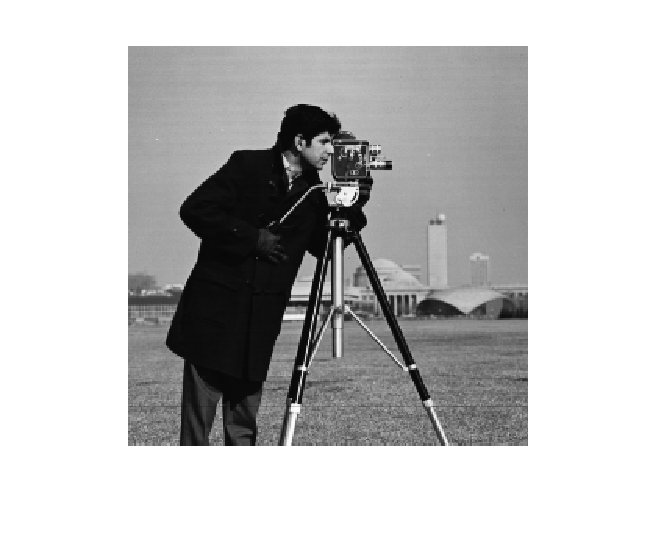
\includegraphics{./Figures/cameramanClean.pdf}
\end{center}
\caption{The MIT camerman, a classic image used in image processing}
\label{fig:cameramanclean}
\end{figure}
You should see the image shown in Figure \ref{fig:cameramanclean}. Now pass this image to our entropy function to calculate the entropy of the image data. We get a value of $7.009$. If this image were uniformily random, the entropy would be $8$, since each pixel is an $8$ bit number, and a uniform distribution of integers between $1$ and $128 = 2^8$ will have an entropy of $8$ (you can verify this fairly easily using the equation we defined above). This implies that the image has potential for compression.

\begin{problem}
Now rewrite your function without using loops. This is an example of using vectorization to speed up algorithms. Use the cameraman image to test how much faster this function is than your original.
\end{problem}

\section*{Chebyshev Polynomials}

One special type of polynomials are the Chebyshev Polynomials. They are useful in a variety of applications including:
\begin{itemize}
\item Evaluating integrals using Gaussian quadrature
\item Solving PDE's
\item Speeding up iterative matrix methods (finding eigenvalues and solving large systems)
\item minimizing interpolation error
\end{itemize}

We will explain many of the these applications in subsequent chapters. The purpose of this example is primarily to give you a real opportunity to investigate ways to speed a process up on your own.

The value of the n-th Chebyshev Polynomials can be described by the following mathematical formulae\footnotemark :
\[
T_n(x) = cos(n cos^{-1}(x))
\]

\[
T_n(x) = 2xT_{n-1}(x) - T_{n-2}(x), T_0(x) = 1, T_1(x) = x
\]

\footnotetext{Technically the first formula only works on the interval $[-1,1]$. There are more general formulae, piecewise defined using $\cosh$ outside of $[-1,1]$, but for this exercise we'll stick to the above definition.}

\begin{problem}
Write a function that accepts a vector $x_0$ of values in $[-1,1]$ and a degree $n$.  The function should return a array evaluting each entry of $x_0$ at every chebeshev polynomial of degree $n$ or less. Essentially, the n-th column of the output should contain the $n-1$ Chebyshev Polynomial evaluated at $x_0$. 
You will be writing four slightly different versions of this function.
\begin{enumerate}
\item Use only for loops and Python's \li{math} library (you will need two for loops).
\item Same as previous, but replacing one for loop with a list comprehension.
\item Use \li{sp.vectorize} to vectorize Python's \li{math} functions.  Keep the list comprehension from previous part.
\item Use SciPy's optimized $\cos$ and $\arccos$ functions.
\end{enumerate}
Make this function as fast as possible (this is the point of the exercise, writing a function solving this problem shouldn't be too difficult anymore). You should investigate both mathematical definitions, and how the number of {\tt for} loops affects the speed. Explain how you optimized your function, and why other implementations would be slower.
\end{problem}


\lab{Applications}{Recursive Functions}{Recursive Functions}

\objective{We will briefly discuss an important technique in programming known as recursion.}

A recursive function is one that calls itself.  A nice example of a recursive function is the Euclidean Algorithm for calculating the greatest common divisor of two integers, $a$ and $b$.

\begin{lstlisting}[style=python]
def gcd(a, b):
    assert a >= b and b >= 0
    if b == 0:
        return a
    else:
        return gcd(b, a%b) 
\end{lstlisting}

All recursive functions have to meet several criteria.  If any one of the criteria are violated, the recursion either doesn't happen at all or the recursion will never terminate (an infinite loop).
\begin{itemize}
 \item Base case.  This defines the stopping criteria for the recursive method.  In the method above, the base case is \li{if b==0}.
 \item Recursive call.  The function should call itself at sometime with new inputs.  The recursive call is \li{return gcd(b, a\%b)}.
 \item Convergence. The recursion must advance toward the base case.  This ensures we don't infinitely recurse.  Study the method above to see how it converges to the base case (try putting print statements in the method if help is needed).
\end{itemize}

Here's a simple combinatoric example. Suppose our goal is to enumerate every possible way to select $n=6$ numbers out of a list of ten numbers (note that we are talking combinations not permutations). We could use some sort of complicated \li{for} loop structure.  It would require six loops to accomplish the task.

\begin{lstlisting}
for i in ...:
    for j in ...:
        for k in ...:
            for l in ...:
            .
            .
            .
\end{lstlisting}

However, we wish to stress emphatically, that this is rarely the right way to do any problem.  What would happen if $n$ were large? Once you write more than three nested \li{for} loops you are probably skirting on the edges of intractability.  In fact, any time you attack a problem that suggests this approach you are likely attacking a problem that is inherently intractable. Sometimes, a problem of this type can be more elegantly solved using recursion.

For example in our combinatorics problem above we could write something like the following.  The solution uses recursion to make the solution more simple.

\lstinputlisting[style=fromfile]{./Source/combinations.py}

\begin{problem}
Note that just because a recursive algorithm exists does not mean that it is the correct way to solve the problem. Computing $n!$, for example, is very inefficient.   The factorial example makes this readily evident. Program a recursive function that will calculate $n!$.  For each step of the recursion, have it print what quantities are being calculated. Time it for increasing values of $n$ (but not too large).  Why is computing $n!$ recursively bad?Generally speaking recursion slows things down, so it should be avoided when possible.
\end{problem}

\begin{problem}
Write a non-recursive version of the \li{gcd} function at the beginning of this lab.  Time the performance of the recursive and non-recursive versions for larger and larger values of $a \geq b$. Generally, recursion does slow things down.  However, sometimes recursion is the best method for solving a problem.
\end{problem}


\begin{problem}
Use recursion to calculate the determinant of an array using cofactor expansions (this is known as Laplace's formula). The correct solution should only be several lines of code. You can see how simple recursive programs can be. Now time your function and compare its performance to finding the determinant using the LU decomposition that you wrote earlier. How does it fare? You will probably notice that the recursive method is much slower for even moderate values of $n$. Why is this? Laplace's formula is $O(n!)$, so even though it's very easy to code it's terribly inefficient in general.
\end{problem}
%We need a profiler lab here.

\end{python}

\begin{matlab}
\lab{Algorithms}{Nested and Anonymous Functions}{Nested and Anonymous Functions}

\objective{Learn about nested and anonymous functions}

\section*{Nested functions}

While writing complicated functions it is often easiest to break up tasks. For this purpose we can write functions inside functions that will perform specific tasks without having to create an entirely new m-file. Here's an example of psudocode for newton's method:

\begin{lstlisting}[style=matlab]
function out = Newtons(f,x0)
.
.
.
%%Here we perform Newton's method. It will need f' so we write a nested function
  function out2 = deriv(x)
    %%here we numerically calculate the derivative of f.
  end
end
\end{lstlisting}

One of the benefits of this method is that we do not have to pass the function to calculate the derivative. Since deriv is nested inside the Newtons function it can access variables inside the scope of Newton, including f. While in this simple example that probably isn't terribly important, it can be much faster in some applications.

\section*{Anonymous Functions and Function Handles}

An anonymous function allows us to create simple, one line functions. The syntax is illustrated by this example:

\begin{lstlisting}[style=matlab]
sincos = @(x) sin(x) + cos(x);
\end{lstlisting}

Now we can find the value of $sin(x) + cos(x)$ by simply typing $sincos(x)$.

Additionally, we can use anonymous functions to capture ``snapshots'' of data. This example might help:

\begin{lstlisting}[style=matlab]
c = [1 2 3];
f = @(x) c*[1;x;x^2];
c = rand(1,3);
g = @(x) c*[1;x;x^2];
\end{lstlisting}

Here, even though c has been changed f will still output $1 + 2x + 3x^2$.

Oftentimes in real applications we are attempting to do operations on a function. Examples would include root finding, minimization, integration or solving differential equations. Because of this MATLAB has structure that allows us to create functions that accept other functions as input. These types of functions are known as function functions (type in \li{help funfun} to see some examples).

This is often the motivation for using anonymous functions. When we pass any function into a function function we have to pass a function handle (which specifies which argument is variable), and we often do this using the anonymous function structure. For example:

\begin{lstlisting}[style=matlab]
quad(@(x) exp(-x^2/2),0,2)
\end{lstlisting}

This line of code will calculate the integral of $e^{-\frac{x^2}{2}}$ between zero and two. Here we used an anonymous function to get the job done. Note that in creating an anonymous function we are technically creating a function handle, so (using our anonymous function) it's ok to write \li{quad(sincos,0,2)} but it's not ok to write \li{quad(sin,0,2)}.

\begin{problem}
Create a function that accepts a number n, creates a random polynomial of degree n and then finds a zero of the polynomial. If there is no zero then have the function instead return a local minimum. You will need to create function handles and use the built-in function \li{fzero}.
\end{problem}

\begin{problem}
The Lambert W-function is defined as the inverse of the function $f(x) = xe^x$. The W-function has important applications in atomic physics and differential equations. It has no closed-form solution. Create a function that estimates the Lambert W-function (you'll need to use \li{fzero} again).
\end{problem}

\begin{problem}
	Read the help file on the function \li{ode45}. Use \li{ode45} to find the solution of the differential equation:
	\[
		x'' = -3x \hspace{5 mm} x(0) = 1 \hspace{5mm} x'(0) = 0
	\]
	
	To do this, you will want to convert the higher order system into a lower order system of more variables. Try letting $x_1 = x$ and $x_2 = x'$.
	Now plot the output. What do you find? Is this what you expect?
\end{problem}

\begin{problem}
Newton's method is an iterative root-finding method. It generally converges very quickly, and is very important in non-linear optimization. Newton's method starts with an initial guess $x_0$ for a root and then calculates the next guess using the following method:
\[
x_{i+1} = x_i - \frac{f(x_i)}{f'(x_i)}
\]
This procedure repeats until a tolerance is reached (either $x_i - x_{i+1}$ or $f(x_{i+1})$ is small enough)
One of the important advantages to Newton's method as opposed to functions like fzero is that they are more robust when functions have asymptotes (try to use fzero on \li{tan} to see this). Also, Newton's method is generally much faster, and is generalizable to higher dimensions.
Write your own Newton's method. Have it accept as arguments f, f', $x_0$ and tol. Remember that f and f' (which you'll probably have to name something like df or fPrime) will be function handles that are passed in. Hint: Use a while loop that tests for reaching the tolerances.
\end{problem}

\lab{Applications}{Speeding up MATLAB Functions: Vectorization}{Vectorization}

\objective{Demonstrates the importance of vectorization in MATLAB.}

This lab introduces two applied topics (Information Entropy and Chebyshev Polynomials) to explore how we can make functions faster through vectorization.  There are two primary motivations behind vectorizing code.  First, vectorized code is often much clearer and more concise than non-vectorized code.  The second, much larger motivation is performance.  Vectorized code is often magnitudes faster than non-vectorized code.  

The concept behind vectorizing code is move away from operating on one element at a time to operating on entire collections of elements at once.  This section will focus specifically on reducing the number of for loops in our program.  Let us look at two examples of functions that would be really useful if could vectorize them to make them execute faster.

\section*{Information Entropy}

Information entropy is loosely defined as the amount of information that is encoded in each bit of a signal. It is directly related to amount of compression that a signal can undergo without loss.

For example, suppose that our signal is an infinite string ``AAAAAAA...'' Since the signal never changes each bit offers no new information. Thus the entropy in this case is zero.

On the other hand, we assign a truly random uniform binary source an entropy of one (such a source may be related to radioactive decay). This is since we have absolutely no clue what the next symbol we read will be.

We can empirically calculate the entropy of a given signal by the following:
\[
H = -\sum_k{p_k log_2(p_k)}
\]
where $p_k$ is the probability of the kth symbol. Note that this fits the two conventions we set above since
\[
-(1log_2(1) + 0 log_2(0)) = 0
\]
\[
-(1/2log_2(1/2) + 1/2log_2(1/2)) = 1
\]

\begin{problem}
Write a function that finds the entropy of a given input vector {\tt v}. You will have to empirically calculate the probability of a given symbol (you should probably let your symbols be integers). This can be done simply using a {\tt for} loop and the {\tt unique} command.
\end{problem}

We can test the entropy function that you just wrote against bit sources to see how ``random'' they are. For example, we can read an image into MATLAB and view it using the following code:
\begin{verbatim}
>> [X map] = imread('cameraman.tif');
>> imshow(X)
\end{verbatim}

\begin{figure}[h!]
\begin{center}
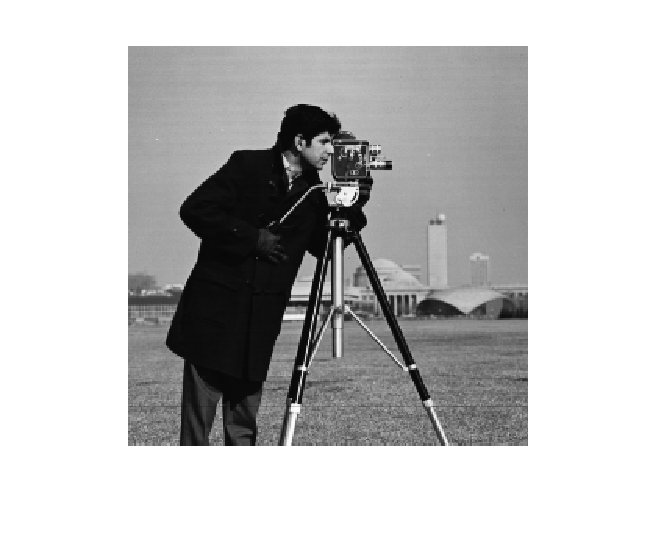
\includegraphics{./Figures/cameramanClean.pdf}
\end{center}
\caption{The MIT camerman, a classic image used in image processing}
\end{figure}
You should see the image shown in figure 1.3. Now run your function on this image (we had to use the code {\tt entropy(X(:)')} to write the signal as a vector). We get a value of $7.0097$. If this image were uniformily random, the entropy would be $8$, since each pixel is an $8$ bit number, and a uniform distribution of integers between $1$ and $128 = 2^8$ will have an entropy of $8$ (you can verify this fairly easily using the equation we defined above). This implies that the image has potential for compression.

\begin{problem}
Now rewrite your function without using loops. This is an example of using vectorization to speed up algorithms. Use the cameraman image to test how much faster this function is than your original.
\end{problem}

\section*{Chebyshev Polynomials}

One special type of polynomials are the Chebyshev Polynomials. They are useful in a variety of applications including:
\begin{itemize}
\item Evaluating integrals using Gaussian quadrature
\item Solving PDE's
\item Speeding up iterative matrix methods (finding eigenvalues and solving large systems)
\item minimizing interpolation error
\end{itemize}

We will explain many of the these applications in subsequent chapters. The purpose of this example is primarily to give you a real opportunity to investigate ways to speed a process up on your own.

The value of the n-th chebyshev polynomials can be described by the following mathematical formulae\footnotemark :
\[
T_n(x) = cos(n cos^{-1}(x))
\]

\[
T_n(x) = 2xT_{n-1}(x) - T_{n-2}(x), T_0(x) = 1, T_1(x) = x
\]

\footnotetext{Technically the first formula only works on the interval $[-1,1]$. There are more general formulae, piecewise defined using $cosh$ outside of $[-1,1]$, but for this exercise we'll stick to the above definition.}

\begin{problem}
Write a function that accepts a vector $x_0$ of values in $[-1,1]$ and a degree $n$, and returns a matrix evaluting each entry of $x_0$ at every chebeshev polynomial of degree $n$ or less. Essentially, the n-th column of the output should contain the $n-1$ Chebyshev Polynomial evaluated at $x_0$. Make this function as fast as possible (this is the point of the exercise, writing a function solving this problem shouldn't be too difficult anymore). You should investigate both mathematical definitions, and how the number of {\tt for} loops effects the speed. Explain how you optimized your function, and why other implementations would be slower.
\end{problem}


\lab{Algorithms}{Recursion and Persistent Variables}{Recursion and Persistent Variables}

\objective{We will briefly discuss an important technique in programming known as recursion. Then we will discuss the use of persistent variables in MATLAB.}

A recursive function is one that calls itself. For example we could write a factorial function as follows:

\begin{lstlisting}[style=matlab]
function out = myFactorial(n)
if n ~= 1
     out = n*factorial(n-1);
else
     out = 1;
end
\end{lstlisting}

This function calculates factorial recursively. It calls \li{factorial(n-1)} until $n = 1$, at which point each function finally terminates.

One critical aspect of this code is the fact that if n == 1, out = 1. This is known as the base case. The base case is the case where the recursion breaks down, or in other words where the function stops calling itself. Every recursive algorithm must have some sort of base case, or else it will call itself indefinitely.

In fact this function only works on positive integers. On any other input the function never terminates. Thus we should modify the function as follows to avoid problems:

\begin{lstlisting}[style=matlab]
function out = myFactorial(n)
if (n <= 0 || rem(1,n) ~= 0)
	error('input must be a positive integer');
end
	
if n ~= 1
     out = n*factorial(n-1);
else
     out = 1;
end
\end{lstlisting}

This practice (of writing code to handle bad user input) is known as defensive programming. It is good to get into this habit.

Here's a simple combinatoric example. Suppose our goal is to enumerate every possible way to select six numbers out of a list of ten (note that we are talking combinations not permutations). We could use some sort of complicated \li{for} loop structure like this:

\begin{lstlisting}[style=matlab]
for i = ...
    for j = ...
        for k = ...
            for l = ...
            .
            .
            .
\end{lstlisting}

However, we wish to stress emphatically, that this is not the right way to do any problem ever. Once you write more than three for loops you are probably skirting on the edges of intractability (in fact, any time you attack a problem that suggests this approach you are likely attacking a problem that is inherently intractable). However, oftentimes such a problem can at least be programmed using recursion.

For example in our combinatorics problem above we could write something like the following:

\begin{lstlisting}[style=matlab]
function out = Combinations(values,k)
%This functions outputs all possible combinations of k elements from the
%vector values.
if min(size(values)) ~= 1
    error('values must be a vector');
end
if k > length(values)
    error('k must be smaller than length(values)');
end
if (k <=0 || mod(k,1) ~= 0) 
    error('k must be a positive integer'); 
end

%Make input vectors column vectors
if size(values,2) > size(values,1)
    values = values';
end

out = []; 
n = length(values); 
if k == 1
    out = values; 
else
    
%This loop iterates through all of elements of the vector values that have at least k
%elements after them (inclusive). For each element it then calls
%Combinations(values(i+1:end),k-1), which returns combinations of size k-1
%for the elements succeeding the current element. This is so that we do not
%get repeats of combinations.
for i = 1:n-(k-1)
    % Calculate the number of possible combinations (to allow proper
    % concatenation in the recursive call.
    numCombs = factorial(n-i)/((factorial(k-1))*(factorial(n-i-(k-1))));
    %This is the recursive call.
    out = [out;[values(i)*ones(numCombs,1), Combinations(values(i+1:end),k-1)]];
end
end
\end{lstlisting}

This solution utilizes recursion to make the coding much more simple. Write this code up and understand why it does what it does, and how the recursion works.

One note of importance: just because a recursive algorithm exists does not mean that it is the correct way to solve the problem. The factorial example makes this readily evident. Generally speaking recursion slows things down, so it should be avoided when possible. However, it can provide elegant solutions to difficult problems, and is a good arrow to have in your quiver.

\begin{problem}
Use recursion to calculate the determinant of a matrix using cofactor expansions (this is known as Laplace's formula). This can be done in four lines. You can see how simple recursive programs can be. Now time your function and compare its performance to finding the determinant using the LU decomposition that you wrote earlier. How does it fare? You will probably notice that the recursive method is much slower for even moderate values of n. Why is this? Laplace's formula is $O(n!)$, so even though it's very easy to code it's terribly ineffective in general.
\end{problem}

\section*{Persistent Variables}

One of the crucial concepts in computer programming is known as scoping. A variable's scope is the function that it lives in. When we write functions the only variables that we have to worry about are the ones that are passed into it. This is because my function has its own scope. A variable that only lives in a specific function (as most variables should) is known as a local variable.

Persistent variables are a tool that MATLAB uses to ease program complexity. A local variable that is declared to be persistent will have the same value the next time the parent function is called. We will illustrate using a function that calculates the fibonacci numbers. In this example we will also practice using recursive functions.

Write the following function:

\begin{lstlisting}[style=matlab]
function out = fib1(a,b,n)
%% calculate the nth fibonacci number using the seeds a,b
if n ==1
	out = a;
else if n == 2
        out = b;
else
        out = fib1(a,b,n-1) + fib1(a,b,n-2);
end
\end{lstlisting}

This function is very easy to read, and directly applies the recursive definition of the fibonacci sequence. However, there is a problem. Consider the function calls made for $n=5, a = 1, b = 1$:

\begin{align*}
fib(5) &= fib(4) + fib(3) = (fib(3) + fib(2)) + (fib(2) + fib(1)) \\
       &= ((fib(2) + fib(1)) + fib(2)) + (fib(2) + fib(1))
\end{align*}

It is clear that many calculations are being repeated unnecessarily. One possible way to solve this problem is to use a \li{for} loop instead. Try writing the following function:

\begin{lstlisting}[style=matlab]
function out = fib2(a,b,n)
%% calculate the nth fibonacci number using the seeds a,b
if n == 1
	out = a;
else if n == 2
        out = b;
else
        x = [a b];
        for i = 1:n-2
            x = [b sum(x)];
        end
        out = x(2);
end
\end{lstlisting}

This version has the advantage that there are no repeated calculations. However, suppose that we are expecting a and b to usually remain the same. Each time \li{fib} was called all of the calculations would have to be redone. This is where persistent variable can be useful. If a variable is declared persistent its value will be stored for the next time the function is called. In this example we can store the entire fibonacci sequence as a persistent variable and only recalculate as necessary. The following code implements this approach:

\begin{lstlisting}[style=matlab]
function out = fib3(a,b,n)
%% calculate the nth fibonacci number using the seeds a,b
persistent f
if length(f) < 2 || f(1) ~= a || f(2) ~= b
    f = [a b];
end
for k = (length(f) + 1):n
    f(k) = f(k-2) + f(k-1);
end
out = f(n);
\end{lstlisting}

Test this code out. Try testing its performance against the other versions (you could try calculating the same fibonacci number several thousand times). You should see a significant difference.

We finish this section with a word of caution. Persistent variables require significant overhead, and accessing them is much slower than accessing normal variables. They should accordingly be used sparingly.

\begin{problem}
Use persistent variables to speed up the calculations of the \li{expss} function that you wrote in chapter one (hint: certain operations, such as factorial, are costly). Test your new function's performance against the old one. How does it perform?
\end{problem}

\begin{problem}
Compare the performance of the \li{fib3} versus \li{fib2}, when the seeds are random every time. You should run it several thousand times in your test. What do you notice? \li{fib3} is much slower because accessing a persistent variable is very costly. This reminds us that using persistent variables should be avoided in most situations.
\end{problem}

\lab{Algorithms}{Profiler and Structs}{Profiler and Structs}

\objective{Learn how to use Structs in MATLAB, and how to use the profiler to optimize code.}

Often physical models have many parameters. MATLAB offers a simple way to handle groups of parameters, known as a structure. Try the following:

\begin{lstlisting}[style=matlab]
P.a = 10;
P.b = 3;
\end{lstlisting}

Now instead of passing the parameters a and b, you can simply pass the structure P and then access the parameters. This makes our functions much easier to use, and it makes paramters much easier to manipulate.

For example, consider the following dynamical system (known as the Lotka-Volterra equation):

\begin{equation}
    \begin{split}
        R'(t) &=aR(t)-bR(t)F(t)\\
        F'(t) &=cR(t)F(t)-dF(t)
    \end{split}\notag
\end{equation}

This system represents predator-prey interaction. $R$ is the number of prey, and $F$ is the number of predators. Suppose that we want to run this model with varying parameters. We can do this very easily with structures:

\begin{lstlisting}[style=matlab]
P.a = 10;
P.b = 3;
P.c = 2;
P.d = 1;
f = @(t,x) [P.a*x(1)-P.b*x(1)*x(2); P.c*x(1)*x(2) - P.d*x(2)];
[t y] = ode45(f,[0 10],[7;7]);
\end{lstlisting}

\begin{problem}
Write a function Lotka(t,P) that plots the solution of the Lotka-Volterra equation on the interval $[0,t]$ using parameters stored in structure P. 
\end{problem}

Next we will introduce a powerful tool in code optimization: the Profiler. At the command line in MATLAB type ``profile viewer''. You should see a window that looks like this:

\begin{center}
\includegraphics[scale = .7]{./Figures/blankProfile}
\end{center}

This is the profiler. Now run Lotka(25,P), with some P that you set previously. You should get output that looks like this:

\begin{center}
\includegraphics[scale = .7]{./Figures/LotkaProfile}
\end{center}

Explore this window. Try clicking on some of the links. You can view how long MATLAB spent calling different functions trying to solve this differential equation.

This information can be incredibly valuable in speeding up functions. You can clearly see what functions are being called, and where speed-up needs to occur.

\begin{problem}
Write the following function:
\begin{lstlisting}[style=matlab]
function I = interpquad(x,y)
%%This function interpolates sorted data points and then integrates the function found by interpolation
method = 'pchip';
I = quad(@interpolant,x(1),x(end));

    function f = interpolant(t)
            f = interp1(x,y,t,method); 
\end{lstlisting}

Run the profiler on this function, using the following code to generate your random data:

\begin{lstlisting}[style=matlab]
x = 1:.2:10;
y = log(x) + rand(size(x))-.5
\end{lstlisting}

What do you notice? How many times is \li{interp1} called? This is a problem, since \li{interp1} has to calculate the interpolating function every time it is called. Look up the 'pp' option in the help documentation of \li{interp1}. Apply this option so that \li{interp1} is only called once. How much does performance improve?
\end{problem}



\end{matlab}

%-----------------------------------------------------------
%These labs cover the basics of differentiation, Newton's method and a number of related applications. These are combined labs

\lab{Algorithms}{Numerical Derivatives}{Numerical Derivatives}

\objective{Understand and implement finite difference approximations of the derivative. This lab focuses on functions from $\mathbb{R} \to \mathbb{R}$, while a later lab focuses on the multidimensional case.}

The derivative of a function at a point is formally defined as

\begin{equation}
\label{eqn:deriv}
f'(x) = \lim_{h\rightarrow 0} \frac{f(x + h)-f(x)}{h}
\end{equation}

In most real world applications we will be solving problems using computers. How does a computer calculate a limit? In short it can't. Computers can only approximate functions at specific points, and the notion of a limit graces infinity in a way that a computer never can.

So how can we use a computer to find the derivative of a function, particularly when we can't differentiate the function by hand? We use methods known as finite difference methods. For example suppose that in equation \ref{eqn:deriv}, instead of taking a limit we just pick a particularly small value for h. Then we have

\begin{equation*}
f'(x) \approx \frac{f(x + h)-f(x)}{h}
\end{equation*}

This is known as the first order forward difference approximation of the derivative.

How do we know the quality of this approximation? We can use Taylor's formula to find

\begin{equation*}
f(x_0 + h) = f(x_0) + hf'(x_0) + h^2/2 f''(\xi),\hspace{5mm} \xi \in (x_0,x_0 + h)
\end{equation*}

Which can be also expressed as

\begin{equation*}
f'(x_0) = \frac{f(x_0 + h) - f(x)}{h} + \frac{h}{2}
f''(\xi) = \frac{f(x_0 + h) - f(x)}{h} + O(h)
\end{equation*}

Here we use the big-O notation to denote that the errors are bounded by some constant multiplied by $h$.

We can use Taylor expansions to find approximations that have different big-O error bounds, up to any polynomial of arbitrary degree. The following tables offer the coefficients for forward, and centered difference schemes.

\begin{table}
\begin{center}
\begin{tabular}{|c|c|c|c|c|c|c|c|c|}
\hline
Derivative & Accuracy & -3 & -2 & -1 & 0 & 1 & 2 & 3 \\ \hline
 & 2 & & & -1/2 & 0 & 1/2 & & \\ \cline{2-9}
 1 & 4 & & 1/12 & -2/3 &  0 & 2/3 & -1/12 & \\ \cline{2-9}
  & 6 & -1/60 & 3/20 & -3/4 & 0 & 3/4 & -3/20 & 1/60 \\ \hline
  & 2 & & & 1 & -2 & 1 & & \\ \cline{2-9}
 2 & 4 & & -1/12 & 4/3 &  -5/2 & 4/3 & -1/12 & \\ \cline{2-9}
  & 6 & 1/90 & -3/20 & 3/2 & -49/18 & 3/2 & -3/20 & 1/90 \\ \hline
\end{tabular}
\caption{Centered Difference Coefficients}
\label{Table:CDiff}
\end{center}
\end{table}

\begin{table}
\begin{center}
\begin{tabular}{|c|c|c|c|c|c|c|}
\hline
Derivative & Accuracy & 0 & 1 & 2 & 3 & 4 \\ \hline
 & 1 & -1 & 1 &  & &  \\ \cline{2-7}
 1 & 2 & -3/2 & 2 & -1/2 & &  \\ \cline{2-7}
  & 3 & -11/6 & 3 & -3/2 & 1/3 &  \\ \hline
  & 1 & 1 & -2 & 1 &  & \\ \cline{2-7}
 2 & 2 & 2 & -5 & 4 &  -1 &  \\ \cline{2-7}
  & 3 & 35/12 & -26/3 & 19/2 & -14/3 & 11/12 \\ \hline
\end{tabular}
\caption{Forward Difference Coefficients}
\label{Table:FDiff}
\end{center}
\end{table}

These tables can be used by simply summing the function evaluations (the number at the top represents how many times $h$ is added to $x$), and then dividing by $h^n$, where $n$ is the degree of the derivative.

So, for example, the centered difference estimate of the second derivative that is $O(h^4)$ is
\begin{equation*}
f''(x) \approx \frac{-1/12(f(x-2h) + f(x+2h)) + 4/3(f(x-h) + f(x+h)) -5/2f(x)}{h^2}
\end{equation*}

Or, the forward difference estimate for the first derivative that is $O(h^2)$ is

\begin{equation*}
f'(x) \approx \frac{-3/2f(x) + 2f(x+h) - 1/2 f(x+2h)}{h}
\end{equation*}

It should be noted that we can convert a forward difference estimate to a backwards difference estimate by using $-h$. So the backwards difference estimate for the first derivative that is $O(h^2)$ is

\begin{equation*}
f'(x) \approx \frac{3/2f(x) - 2f(x-h) + 1/2 f(x-2h)}{h}
\end{equation*}

There are two important observations that you should make about these tables. First, in order to get higher order approximations we need to evaluate the function at more points. This should not be surprising. Second, you should notice that centered difference formulas require less function evaluations to get higher order approximations. However, in certain applications it is not possible to use centered difference formulas, so the backwards and forwards formulas are still very applicable.

One important aspect of this method is selecting an appropriate $h$. The natural temptation is to pick a very very small value. However, this is not always advisable. Note the values in table \ref{Table:FloatingError}, which approximates the derivative of $e(x)$ at $x = 1$:

\begin{table}[h!]
\begin{center}
\begin{tabular}{|cc|}
\hline
h & Error  = $|f'(1)-f'_{app}(1)|$ \\ \hline
1e-1 & 4.5e-3 \\
1e-3 & 4.5305e-7 \\
1e-7 & 5.8587e-11 \\
1e-10 & 6.7274e-7 \\ \hline
\end{tabular}
\caption{Error in numerical derivative, using double precision floating point arithmetic}
\label{Table:FloatingError}
\end{center}
\end{table}

As you can see, the error actually increases as $h$ becomes very small. Why is this? Division by small numbers causes errors in floating point arithmetic. So, be aware that usually the optimal $h$ is of moderately small size. However, in the framework of double floating point arithmetic, this is usually less of a concern.

As a matter of reference, calculating numerical derivatives is an unstable operation. An unstable operation, informally, is one where errors are magnified by the operation. This usually is not an issue, but it's important to know that taking derivatives can amplify errors.

\begin{problem}
Write a function that accepts as inputs: a derivative (first or second), a degree of accuracy ($n$), a type of difference (forward, backward or centered), a function to be differentiated, and a vector of points to differeniate at. Also, allow an optional input of error tolerance. Have the function estimate the derivative with the inputed specifications. Have the function return a vector of the approximate derivative and the number of total function evaluations. Try to minimize the total number of necessary function evaluations. You can have the function output an error if the specified order of derivative or degree were not provided in Table \ref{Table:CDiff} or \ref{Table:FDiff}.
\end{problem}

We note that higher order approximations of the derivative can be derived using the Taylor series and Lagrange polynomials, but generally higher-order approximations are not practically useful as they can often be ill-conditioned.

\begin{problem}
Test the convergence properties claimed in Tables \ref{Table:CDiff} and \ref{Table:FDiff}. Specifically, empirically calculate the order of convergence of a $O(h^2)$ centered difference and a $O(h^3)$ forward difference by calculating the derivative of the sine function at $x=1$. How does it compare to the order of convergence expected?
\end{problem}

\lab{Applications}{Beam Buckling}{Beam Buckling}

\objective{Use finite difference approximations and eigenvalues to approximate the strength of various types of beams.}

In many engineering applications it is desirable to be able to test how strong a structure will be prior to actually building it. In this lab we will explore the strength of a simple beam using mathematical techniques.

We can model a beam supporting a load $P$ by the following equation:

\[
EI \frac{d^2 y}{dx^2} = -P y
\]

\begin{figure}
\begin{center}
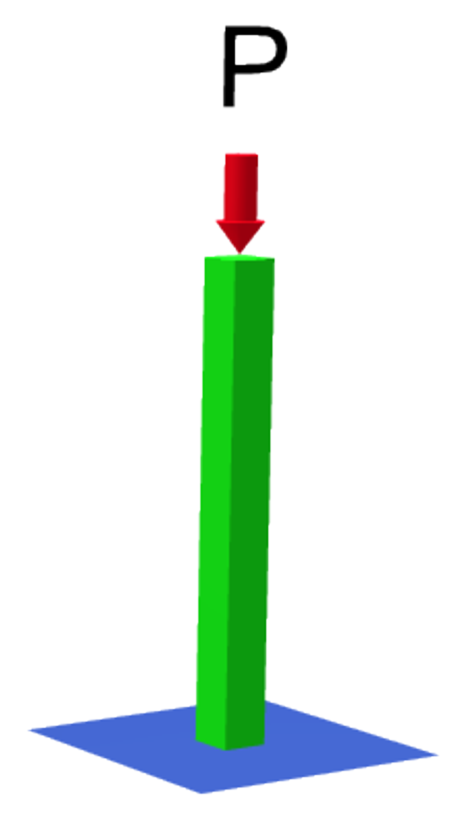
\includegraphics[scale = .3]{./Figures/Buckling.pdf}
\caption{A beam supporting a load $P$}
\label{Fig:Beam}
\end{center}
\end{figure}

This scenario is shown in figure \ref{Fig:Beam}. The variable $x$ is up and down, and $y$ is a lateral displacement (left or right). We have really simplified this problem to two dimensions, but the simplification is still representative in this case. We also have the boundary conditions that:

\[
y(0) = y(L) =0
\]

This specifies that the position of the top and bottom boundaries of the column are fixed (as would be the case in a building). In these equations $L$ is the length of the column, $E$ is known as the elastic modulus (representing the rigidity of the material) and $I$ represents the area moment of inertia (representing how the geometry resists deformation).

We can solve this equation using finite difference approximations. Recall that one approximation of the second derivative of a function is the following:

\[
y''(x_k) = \frac{y(x_k-1) - 2y(x_k) + y(x_{k+1}}{h^2}
\]

So, if we select the points

\[
x_k = \frac{kL}{n}
\]

For $k = 0\ldots n$ then we can rewrite our differential equation in the form:

\[
\frac{EIAy}{h^2} = -Py
\]

Where $y$ is a vector of length $n-1$ representing our function values at all of the $x_k$ (except for $k=0$ and $k=n$, which are determined by the boundary conditions), $h = \frac{L}{n}$ and $A$ is a matrix with $-2$ on the diagonal and $1$ on the super and sub-diagonal, as specified by the finite difference approximation above. Note that we incorporated our boundary conditions in the corners of the matrix (the derivative is only approximated by two terms there, since the third term in each case is the boundary term that is fixed at zero).

Clearly for any value of $P$ the equation has a trivial solution ($y=0$). However, by calculating the eigenvalues we can find the values of $P$ for which the equation has a non-trivial solution. Recall that any multiple of an eigenvector will still be an eigenvector. This means that when $P$ is an eigenvalue there are arbitrarily small non-trivial solutions to the differential equation. This tells us that the trivial solution is actually unstable whenever $P$ is an eigenvalue. Accordingly, the smallest eigenvalue of the system will be the value where the beam buckles and the system fails (in this system all of the eigenvalues turn out to have the correct sign, therefore giving physically meaningful values of $P$).

\begin{problem}
Find the load at which a five foot column of concrete with diameter of one foot will buckle. The modulus of elasticity for concrete is approximately $4.35$ million pounds per square inch. The area moment of inertia in this case is $I = \pi r^4/4$. The only necessary unit conversion is inches to feet (in the modulus of elasticity). The answer should be in $10^7$lbs (you only need to use vectors of moderate size to get an accurate answer: try n=100). What if instead the column is twenty feet long?
\end{problem}

One point of interest is related to the area moment of inertia. Given a fixed amount of material it actually turns out that the area moment of inertia is greater for a hollow tube than a solid column. This tells us that hollow tubes actually have a higher buckling strength than solid ones. In fact, I-beams are actually designed to increase area moment of inertia, which is why they are seen so often in construction.

It turns out we can actually solve this equation analytically. The non-trivial solutions to this type of equation are sines. We can thus deduce, using the chain rule that the eigenvalues of the derivative operator (neglecting the constants E and I) are
\[
\lambda_n = \frac{\pi^2 n^2}{L^2}
\]
for $n \in \mathbb{N}$. Thus we have that the buckling force is:
\[
F = \frac{\pi^2 EI}{L^2}
\]
Which, as you can verify, matches the solution found above very nicely.

So if we can solve this solution analytically why do we bother with the finite difference approximation? Suppose instead that our column is made of two types of concrete, the bottom half with $E = 4.35\times 10^6$ and the other half with$E = 1 \times 10^6$. This type of problem is more difficult to solve analytically. However, if we modify our finite difference equation to compensate for the differences in the material we can still solve the problem. We can re-write the equation:

\[
B A y = -Py
\]
Where B is a matrix with the value of $E I$ at each $x_k$ on the diagonal. So in our example above B would be the following matrix:

\begin{matlab}
\begin{lstlisting}[style=matlab]
B = r^4/4 *diag([4.35*ones(1,50) ones(1,50)])*1e6
\end{lstlisting}
\end{matlab}

\begin{problem}
Suppose that the bottom third of our column is made of aluminum ($E = 10^7$), the middle third is concrete and the top third is made of nylon ($E = 5\times 10^5$). What is the buckling strength of the column? If the order of the materials is changed does this affect the buckling strength?
\end{problem}





\lab{Algorithms}{Multivariate Finite Difference Schemes}{Multivariate Numerical Derivatives}

\objective{Understand how to compute numerically the Jacobian and Hessian of a function.}

The Jacobian is our generalization of the derivative in many dimensions. We can think of it, intuitively, as a tangent plane at a point. The Jacobian is of critical importance in a variety of areas, and we will use it in lab \ref{lab:NewtonsMethod} to find zeros of multivariate functions.

Formally, the Jacobian of a function $f:\mathbb{R}^n \rightarrow \mathbb{R}^m$ is an $m \times n$ matrix. It is defined by the formula:
\begin{equation*}
J_{i,j} = \frac{\partial f_i}{\partial x_j}
\end{equation*}

We can use finite difference approximations to find partial derivatives in the natural manner:
\begin{equation*}
\frac{\partial f}{\partial x_i} (x) \approx \frac{f(x+h e_i)-f(x)}{h}
\end{equation*}
where $e_i$ is a unit vector in the $i$th coordinate (the direction $x_i$). Higher order approximations and centered and backwards differences follow by naturally extending this definition.

\begin{problem}
Write a function \li{Jacobian(func,inputs,dim,h,o)} that accepts a function handle, inputs to the function, the function's dimensions, step size $h$, and option o. Based on the option have the function output the Jacobian using either a centered, forward or backward difference.

Test your function on the following $f: \mathbb{R}^2 \to \mathbb{R}^2$:
\begin{equation*}
f(x_1, x_2) = 
\begin{pmatrix}
e^{x_1} sin(x_2) + x_2^3 \\
3x_2 - cos(x_1)
\end{pmatrix}
\end{equation*} 

Compare your \li{Jacobian} function against the analytically computed derivative on the square $[-1,1] \times [-1,1]$ using ten thousand grid points (100 per side). Which method is faster? What is the maximum error of your function? Make sure to test the different options of your function to maximize performance (including values for $h$, and different types of schemes).
\end{problem}

Given a function from $\mathbb{R}^n \to \mathbb{R}$ sometimes the mixed partial derivatives are useful. In particular the mixed partials will be useful when we study optimization in Volume 2. This information is contained in the Hessian matrix, which is defined as

\begin{equation*}
H_{i,j} = \frac{\partial^2 f}{\partial x_i \partial x_j}
\end{equation*}

We can use the following formula to approximate mixed partial derivatives
\small
\begin{equation*}
\frac{\partial^2 f}{\partial x_i \partial x_j} = \frac{f(x + (e_i + e_j)h) - f(x + (e_i-e_j)h) -f(x + (e_j-e_i)h) + f(x - (e_i + e_j)h)}{4h^2}
\end{equation*}
\normalsize

\begin{problem}
Write a \ProgrammingLanguage function that numerically calculates the Hessian of a given function. Test it on the following function
\begin{equation*}
f(x,y) = (1-x)^2 + 100(y-x^2)^2
\end{equation*}
This function is known as the Rosenbrock Banana function, or Rosenbrock's Valley. It is a common test function for optimization algorithms because it is non-convex and the global minimum is hard to find from certain starting points. A graph is shown in figure \ref{Fig:Rosenbrock}. Compare the output of your function with the analytic solution on the region $[-2,2] \times [0,2]$, using ten thousand points. What is the maximum error of your function?
\end{problem}
\begin{figure}
\begin{center}
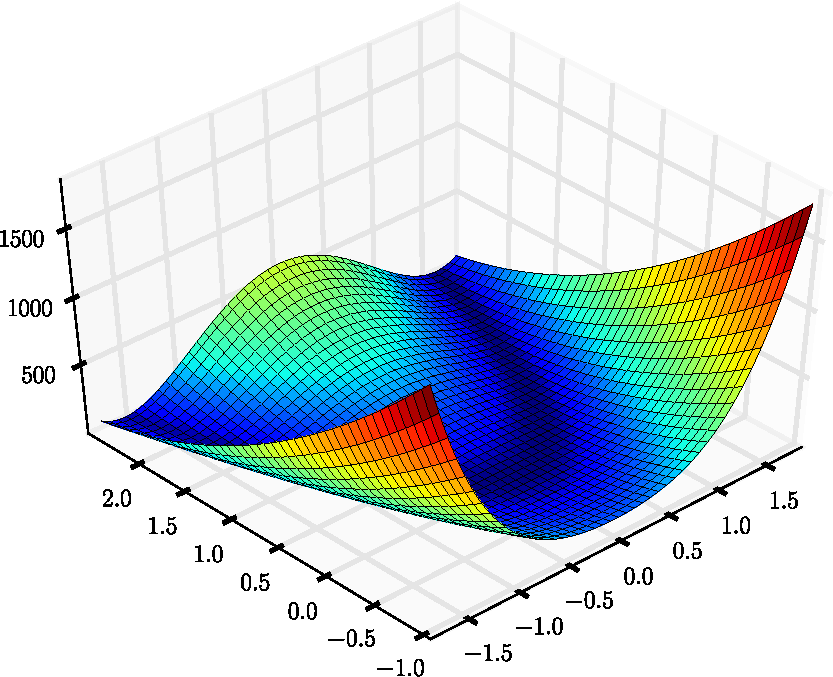
\includegraphics[scale = .8]{./Figures/Rosenbrock}
\caption{The Rosenbrock Banana Function, a common test function in optimization algorithms}
\label{Fig:Rosenbrock}
\end{center}
\end{figure}
\lab{Application}{Image Processing and Filters}{Image Filters}

\objective{Explore Image Filters. In particular, we will explore the Sobel Filter, which uses numerical derivatives to find edges in images.}

One of the primary tools in image processing is the use of filters to identify important information in images. In this section we will implement our own filters and explore applications.

One of the easiest filters to implement is matrix based. In this implementation, the filter that we select is a matrix, which represents how much we want certain pixels to contribute to the output image. Suppose that we choose our filter to be:

\[
A = \begin{pmatrix}
a_{11}&a_{12}&a_{13}\\
a_{21}&a_{22}&a_{23}\\
a_{31}&a_{32}&a_{33}
\end{pmatrix}
\]

We will call our input image (Matrix) B and our ouput image (Matrix) C. This type of filter works according to the following formula:
\[
C_{ij} = \sum_{k=-1}^1 \sum_{m=-1}^1 a_{km}*B_{(i+k,j+m)}
\]

Essentially this computes each pixel of the output image as the weighted sum of the surrounding pixels in the input image. The technical term for this type of operation is a convolution.

\begin{problem}
Write a function that will take as input an arbitrary filter matrix and image and output the filtered image. Note that for these filters to be meaningful they will need to be odd by odd (there are ways to handle even size filters, but we won't handle them here). Have MATLAB return an error message if the filter is not of appropriate size. You may choose how to handle the edges of the image, but we suggest simply copying the edge pixels out.

You can test your function by loading a sample image using the command imread, with a file chosen from the MATLAB demos (pick one from {\tt help imdemos}). You can then apply the identity filter, which is any n by n matrix where n is odd and the only non-zero entry is a one in the very center of the matrix. Use the command {\tt imshow} on both the input and output image. They should be the same.
\end{problem}

So what can we do with these filters? We will show an example of how to apply a gaussian blur using this type of filter. To begin, load the following picture:

\begin{verbatim}
K = imread('cameraman.tif');
imshow(K);
\end{verbatim}

{\tt imshow} should display an image like this one:

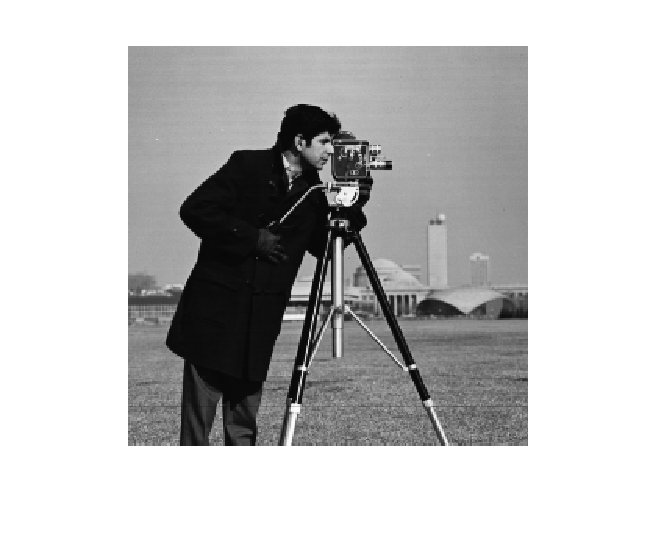
\includegraphics{./Figures/cameramanClean.pdf}

Now that you have a simple filter function try the following filter on this image:

\[
A = \frac{1}{159}\begin{pmatrix}
2&4&5&4&2\\
4&9&12&9&4\\
5&12&15&12&5\\
2&4&5&4&2\\
4&9&12&9&4
\end{pmatrix}
\]

You should get an output that looks something like this:

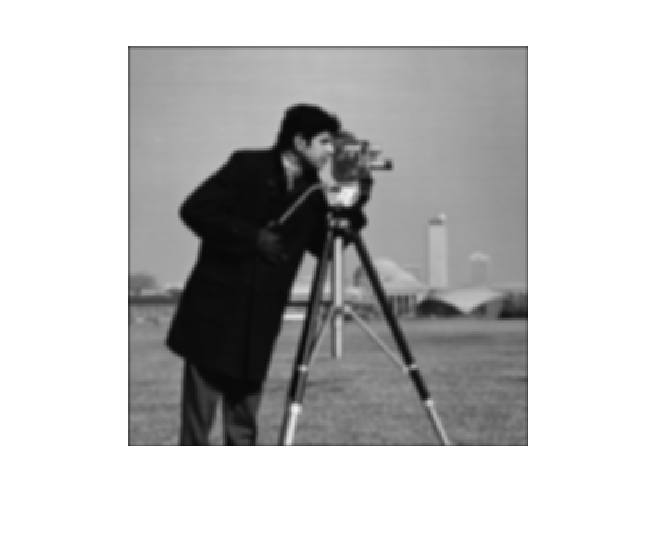
\includegraphics{./Figures/cameramanBlur.pdf}

You can see that the filter blurred the image. This can be very important in trying to wash out images that are ``noisy.''

\begin{problem}

The Sobel Filter is a filter used in edge detection. It works by using a numerical approximation of the gradient to find edges in the image. The filter to find the gradient in the y direction is:

\[
A = \frac{1}{8}\begin{pmatrix}
-1&-2&-1\\
0&0&0\\
1&2&1
\end{pmatrix}
\]

The gradient in the x direction is simply the transpose of that matrix.

Write a simple function that finds the edges of an image using the sobel filter. You will probably need to preprocess the image using the function {\tt im2single}. You will then find the magnitude of the gradient by combining the x and y gradient matrices (what is the correct way to do this?). Lastly, you will need to look for places where the magnitude of the gradient is large enough (the location of edges) by looking at values over a threshold (which you'll also need to find). We found four times the mean of the output image to be pretty good. On the camerman example we had the following output:
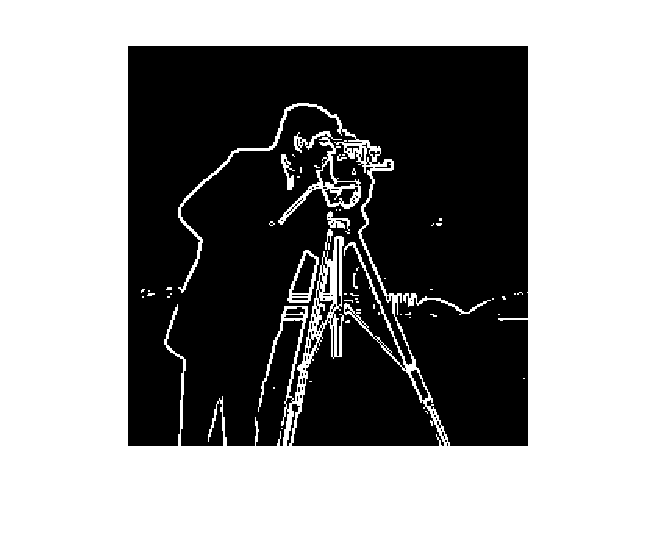
\includegraphics{./Figures/edges.pdf}
\end{problem}


\lab{Application}{Newton's Method}{Newton's Method}

\objective{Understand Newton's Method}

One important technique in technical computing is Newton's method. The goal of Newton's method is to find $x^*$ such that $f(x^*) = 0$. This method is especially important in optimization, where our goal is to find minima and maxima of functions. Newton's method is an iterative method (much like eigenvalue finders: remember how those provably have to be iterative?). Newton's method, in one dimension, is defined as follows:
\[
x_{n+1} = x_n - \frac{f(x_n)}{f'(x_n)}
\]

Essentially Newton's method approximates a function by its tangent line, and then uses the zero of the tangent line as the next guess for $x_n$.
\begin{figure}[h!]
\begin{center}
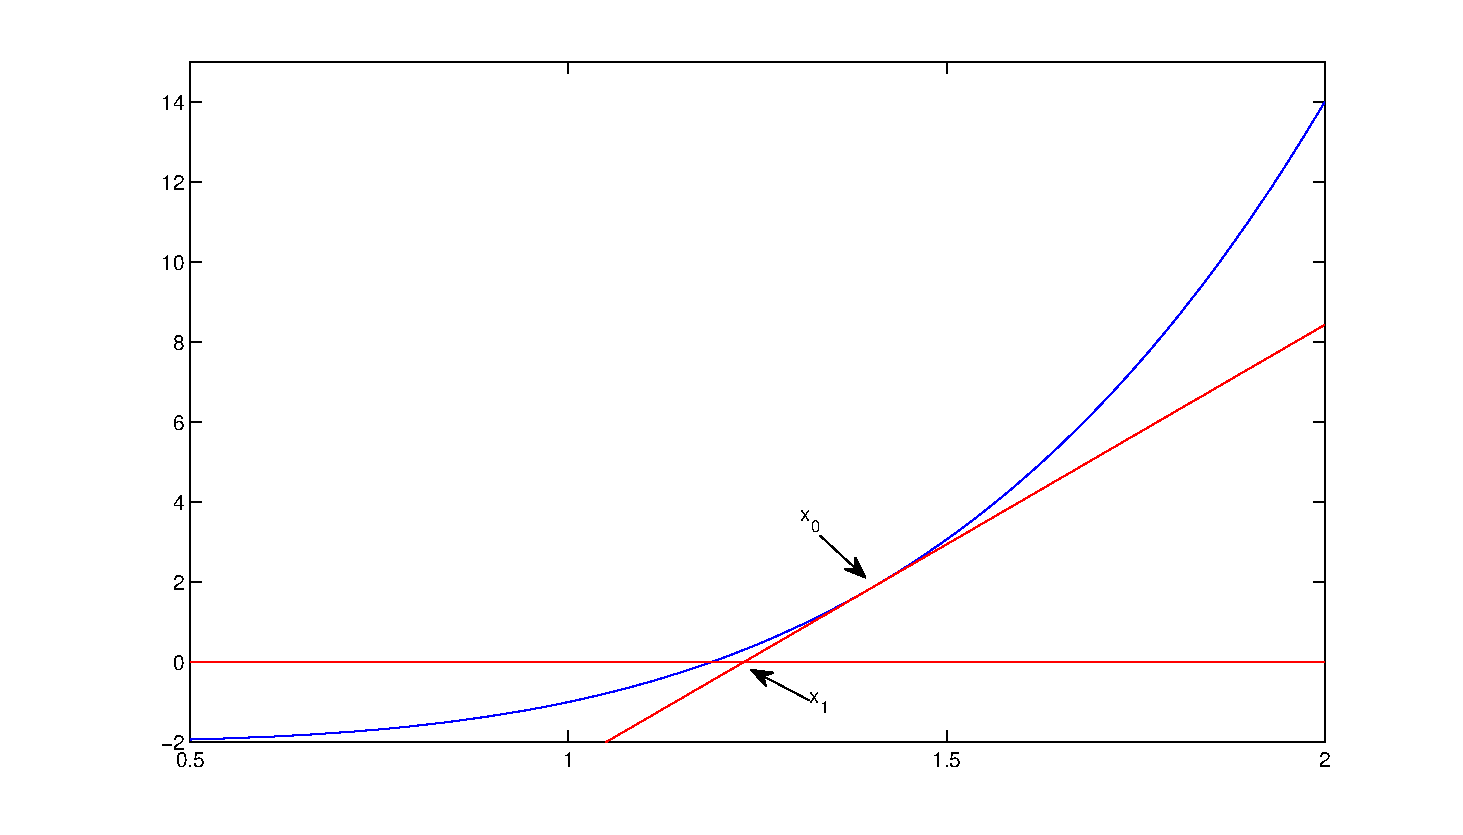
\includegraphics[scale = .5]{./Figures/newton}
\caption{An illustration of how one iteration of Newton's method works}
\end{center}
\end{figure}

Newton's method is powerful because of the speed of convergence. In many cases Newton's method converges to the actual root quadratically, meaning that the error term is squared at every iteration. This fast convergence makes it a very powerful algorithm.

Newton's method does suffer from the flaw that its convergence is dependent upon an initial guess. If the initial guess is not sufficiently close the convergence can be much slower, or may never occur. There are even certain pathological functions for which newton's method will never converge. However, these functions are very rare, and as a rule Newton's method converges very quickly.



\begin{problem}
Modify the Newton's method function that you wrote in chapter one so that it runs whether or not the user inputs a derivative function. \begin{matlab}This will require you to use the commands \li{nargin} and \li{varargin}. If the user does not input a derivative function calculate the derivative numerically.\end{matlab}\begin{python}In python this can be done by defining the derivative function as a keyword argument.  Your function definition will look something like this \li{def new_newton(f, x0, df=None, tol=0.001)}\end{python}

Compare the performance of Newton's method when you input the derivative and when you don't. How well does each converge? Which runs faster? Try the following functions:

\begin{itemize}
\item $cos(x)$
\item $sin(1/x)x^2$
\item $sin(x)/x -x$
\end{itemize}

%When I tested it out in python, hand fed derivatives performed  faster
%cos: 10 times as fast
%sin(1/x)x^2: 7 times as fast
%sin(x)/x - x: 5 times as fast
%sin(x)/x + x: 6 times as fast
%We should specify error bounds and initial guesses for roots
%for some I had trouble with starting guesses producing a zero-valued derivative

%I did not test this in Matlab, and the Matlab version suggests ``$sin(x)/x + x$ might work well.''

\end{problem}

\begin{problem}
Test your newton's method function on $x^{1/3}$. Use random starting points around zero. What do you see? Prove that for any non-zero starting point that newton's method will diverge.
\end{problem}

\begin{problem}
A basin of attraction can be loosely defined as a set that will eventually converge to a specific root. Pick random points on the interval $[-2,2]$ as starting points and apply newton's method to the function $x^3 -2x + 1/2$. Display the basins of attraction for this particular function. What do you observe?

% I don't know anything about attractors, but I graphed mine with the function with these lines
% I thought it helped me visualise it better
% f = lambda x: x**3 - 2*x + 1./2
% df = lambda x: 3*x**2 -2
% x0 = sp.linspace(-2,2,100)
% r = [ newtons2.newtonsMethod(f,df,x,0.001) for x in x0]
% y = [ x**3 - 2*x + 1./2 for x in x0]
% plt.plot(x0,r,x0,y)
% plt.axhline(0,color='black')
% plt.show()

\end{problem}

\begin{problem}
% I found this one very difficult, because scipy does not have a jacobian function, and I kept running into little problems with mine
% However, I did manage to solve it. Perhaps we should supply them a jacobian function
Extend your Newton's method even further so that it will work on systems of equations. Suppose that $F: \mathbb{R}^n \rightarrow \mathbb{R}^n $. The relevant equation is
\[
x_{i+1} = x_i - J^{-1}F(x_i)
\]
\begin{matlab}
 Note that you {\bf should not} calculate the inverse Jacobian. We should just solve for the correct system of equations using backslash. You should be able to make this function work whether or not the user inputs a Jacobian.
\end{matlab}
\begin{python}
Note that you {\bf should not} calculate the inverse Jacobian. \li{sp.solve(A,b)} gives you the solution $x$ to the equation $Ax=b$. Use this fact to calculate $J^{-1}F$ from $J$ and $F$.  You should be able to make this function work whether or not the user inputs a Jacobian. This also means that you will have to implement your own \li{jacobian} function.
\end{python}
\end{problem}


\lab{Applications}{Continuation and Level Sets}{Continuation and Level Sets}

\objective{Not quite sure what to do with this topic.  Most of what I see on continuation seems pretty technical.  Maybe just some level set stuff instead?}
%Needs to be written

\lab{Algorithms}{Broyden's Method}{Broyden's Method}

\objective{Implement Broyden's Method and understand the tradeoff with Newton's Method}

We have already discussed using Newton's method to find the roots of an equation. Newton's method is generally very useful because of its fast convergence properties. However, Newton's method requires computation requires the explicit calculation of the derivative (or respectively jacobian matrix) at each step, which is computationally costly. There is a class of methods known as quasi-Newton methods that modify newton's method so that the derivative (jacobian) does not have to be computed at each step, thus making computations faster. This generally comes at a slower convergence speed, but the increased computation speed can make these methods more effective in many cases.

One quasi-Newton method is known as Broyden's method. We will first discuss the one-dimensional case of Broyden's method: the secant method.

The secant method begins with two initial points that are presumably close to the desired root. We can calculate the equation of the secant line between the two points $x_i$ and $x_{i-1}$ by the following:
\[
y = \frac{f(x_i)-f(x_{i-1})}{x_i-x_{i-1}}(x-x_i) + f(x_i)
\]

Now suppose that we set the next guess of our iterative method to the zero of the secant line, namely:
\[
x_{i+1} = x_i - f(x_i)\frac{x_i-x_{i-1}}{f(x_i)-f(x_{i-1})}
\]

This process is demonstrated in graphically in Figure \ref{Fig:Secant}.  By continuing this process we (in many cases) will converge to the zero of the function. This method does not require knowledge of the derivative and hence is computationally less costly than Newton's method.

This method is shown in pseduocode in Algorithm \ref{Alg:Secant}.

\begin{pseudo}{Secant}{func, x1, x2, tol}
\label{Alg:Secant}
\IF \abs{func(x1)} < tol \THEN
    \RETURN{x1}\\
\IF \abs{func(x2)} < tol \THEN
    \RETURN{x2}\\

\REPEAT 
xnew \GETS x1-func(x1)*\frac{x1-x2}{func(x1)-func(x2)}\\
x1 \GETS x2 \\
x2 \GETS xnew \\
\UNTIL \abs{func(xnew)} < tol \THEN \RETURN{xnew}
\end{pseudo}


\begin{figure}
\begin{center}
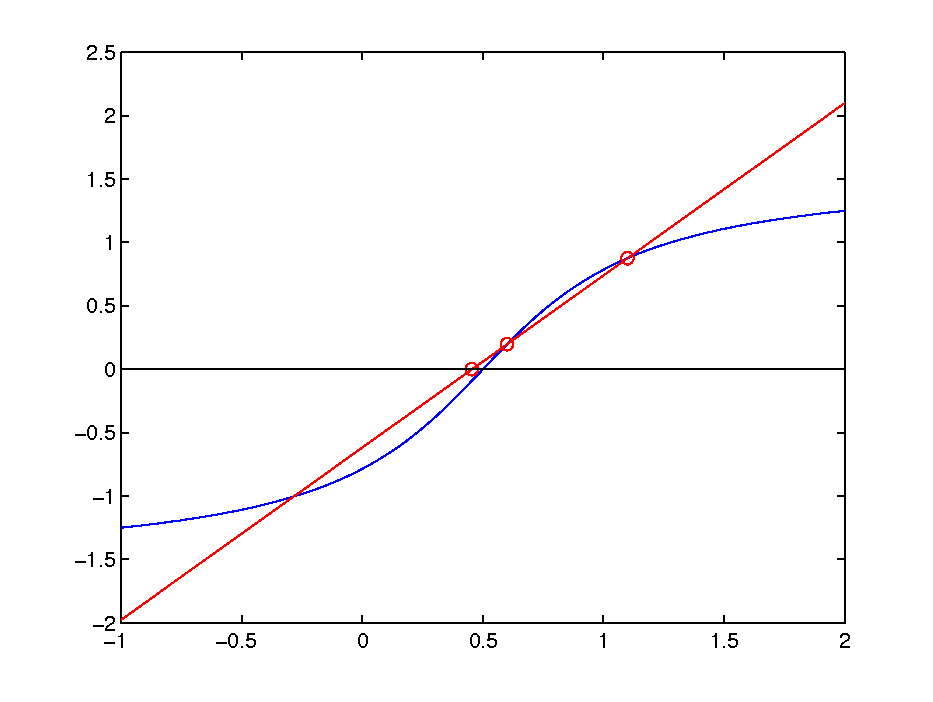
\includegraphics[scale = .5]{./Figures/Broyden_Secant_Method}
\caption{A demonstration of using the secant method to find a point closer to the desired root.}
\label{Fig:Secant}
\end{center}
\end{figure}

\begin{problem}
Write a function that takes as input two initial points and a callable function (a function handle or lambda function) and return the zero of the function between the two given points.  If unable to calculate the zero of the function, raise an error.  Also, estimate the exponent of convergence using a log-scaled plot when you use your function to estimate the zero of $e^x-2$. The actual value of the exponent of convergence is a value known as the golden ratio, which can be written:
\[
\phi = \frac{1 + \sqrt{5}}{2} \approx 1.62
\]
The golden ratio shows up in a variety of settings, but we won't discuss them here.
\end{problem}

It is interesting to look at the secant method as a specific case of Newton's method, where we have chosen to approximate the derivative using the secant line between our current set of points.

By combining the secant and the bisection method we obtain a more robust method that is guaranteed to converge. This method is known as the \emph{regula falsi} method. The regula falsi method is thousands of years old, dating to at least the third century BC.

The regula falsi method assumes that we have initial points $x_0$ and $x_1$ such that $f(x_0) < 0 < f(x_1)$. We then use the root of the secant line to find our new point $x_2$. However, we then choose to keep $x_1$ only if $\mbox{sgn}(f(x_2)) \neq \mbox{sgn}(f(x_1))$, otherwise we keep $x_0$. In this manner we can combine the robustness of the bisection method with some of the faster convergence properties of the secant method.

\begin{problem}
Write a function implementing the regula falsi method. Compare convergence speed with the secant method on the functions:
\begin{align*}
f(x) &= e^x-1\\
f(x) &= cos(x)\\
f(x) &= x^7\\
\end{align*}
\end{problem}

%-----------------------Need Clarification (jacobian)-----------------------
The generalization of the secant method to multiple dimensions is called Broyden's Method.  If we have the point $x_k$ and the Jacobian $J_k$ at that point we can use the following equation to select our guess for the zero of the function:
\begin{equation} \label{Eq:BroydenSolve}
J_k \Delta x = -F(x_k)
\end{equation}

Where $\Delta x = x_{k+1}-x_k$. This is precisely Newton's method. However, since calculating the Jacobian at each step is costly, we instead use a generalization of secant lines to estimate the Jacobian (just as we used a secant line to approximate the derivative in the one-dimensional case).

The generalization for using secant lines is as follows: If we have points $x_k$ and $x_{k-1}$ then the Jacobian $J_k$ at the point $x_k$ will approximately satisfy the following equation:
\begin{equation}
J_k (x_k-x_{k-1}) \approx F(x_k) - F(x_{k-1})
\end{equation}
In the one dimensional problem we can use this equation to exactly specify the value $J_k$ (this is simply a finite difference approximation of the derivative). However, in multiple dimensions, the equation will be underdetermined (i.e. many $J_k$'s will satisfy the equation). However, suppose that we have a previous estimate of the Jacobian $J_{k-1}$ at the point $J_{k-1}$. We can then find the solution to the multi-dimensional secant equation above that minimizes $\|J_{k-1}-J_k\|$. This requirement is uniquely fulfilled by the following:
\begin{equation} \label{Eq:BroydenJacobian}
J_k = J_{k-1} + \frac{\Delta F-J_{k-1} \Delta x}{\|\Delta x\|^2}\Delta x^T
\end{equation}

In this equation the $\Delta F = F(x_k)-F(x_{k-1})$ and $\Delta x = x_k-x_{k-1}$. Intuitively, we are using the secant equation to make a rank-one update on the Jacobian at each step of the algorithm.

After we have obtained our secant line approximation of the jacobian (Equation \ref{Eq:BroydenJacobian}) we can apply Equation \ref{Eq:BroydenSolve} to find $x_{k+1}$. We can then repeat this process until we have (presumably) converged to a zero of the function. Pseudocode is shown in Algorithm \ref{Alg:Broyden}:

\begin{pseudo}{Broyden}{func,x1,x2,tol}
\label{Alg:Broyden}
\IF \abs{func(x1)} < tol \THEN
    \RETURN{x1}\\
\IF \abs{func(x2)} < tol \THEN
    \RETURN{x2}\\

J \GETS Jacobian(x1) \\

\REPEAT 
F1 \GETS func(x1) \\
F2 \GETS func(x2) \\
\Delta x \GETS x2 - x1 \\
J \GETS J + \frac{F2-F1-J \Delta x}{\|\Delta x \|^2}\Delta x^T \\
xnew \GETS J \backslash (-F2) + x2 \\
x1 \GETS x2 \\
x2 \GETS xnew \\
\UNTIL \abs{func(xnew)} < tol \THEN \RETURN{xnew}
\end{pseudo}

\begin{problem}
Write code implementing Broyden's method. Test it on the function:
\[
f(x,y,z) = cos(xy) + xz^3 + y^2 - y + x^2 + z + x
\]
\end{problem}

We can often make Broyden's method faster using the Sherman-Morrison Woodbury Formula. This formula allows us to efficiently calculate the inverse of a matrix when we add a low rank update to that matrix. After manipulation of the Sherman-Morrison Woodbury Formula we obtain the following:

\[
J_k^{-1} = J_{k-1}^{-1} + \frac{\Delta x - J_{k-1}^{-1}\Delta F}{\Delta x^T J_{k-1}^{-1}}
\]

Thus, we can calculate the inverse of the jacobian in the first step of our algorithm and then calculate an update to the inverse at each step using the above formula.

\begin{problem}
Implement this modification in a new file. Now compare the two versions of Broyden's method on the function above. Which is faster? Are there cases where one implementation is better than the other?
\end{problem}
%Needs to be translated (RDG)
\lab{Applications}{Julia Sets and Basins of Attraction}{Julia Sets}

\objective{Understand definition of basin of attraction.  Basic understanding of Julia Sets.}

%\begin{itemize}
%\item Recall Newton's method
%\item Different seed values for Newton yield different roots.
%\item Definition of basin of attraction.
%\end{itemize}

Recall Newton's method for finding the roots of a function in one variable.  Given the function $f$ and a seed value $x_0$, we can iteratively find a root:
\[
x_{n+1} = x_n - \frac{f(x_n)}{f'(x_n)}
\]
We have shown in previous sections that this method will converge very quickly to a root.  For example, given
\[
f(x) = x^2 + x -2
\]
and a seed value of $x_0 = 4$, after only 4 iterations we are about as close to the true root at $1$ as we would like.  What happens, however, when we choose a different seed value, say $x_0 = -4$?  Going through the Newton iterations, we notice that we quickly converge to the other root of the function, $-2$.

\begin{figure}
\begin{center}
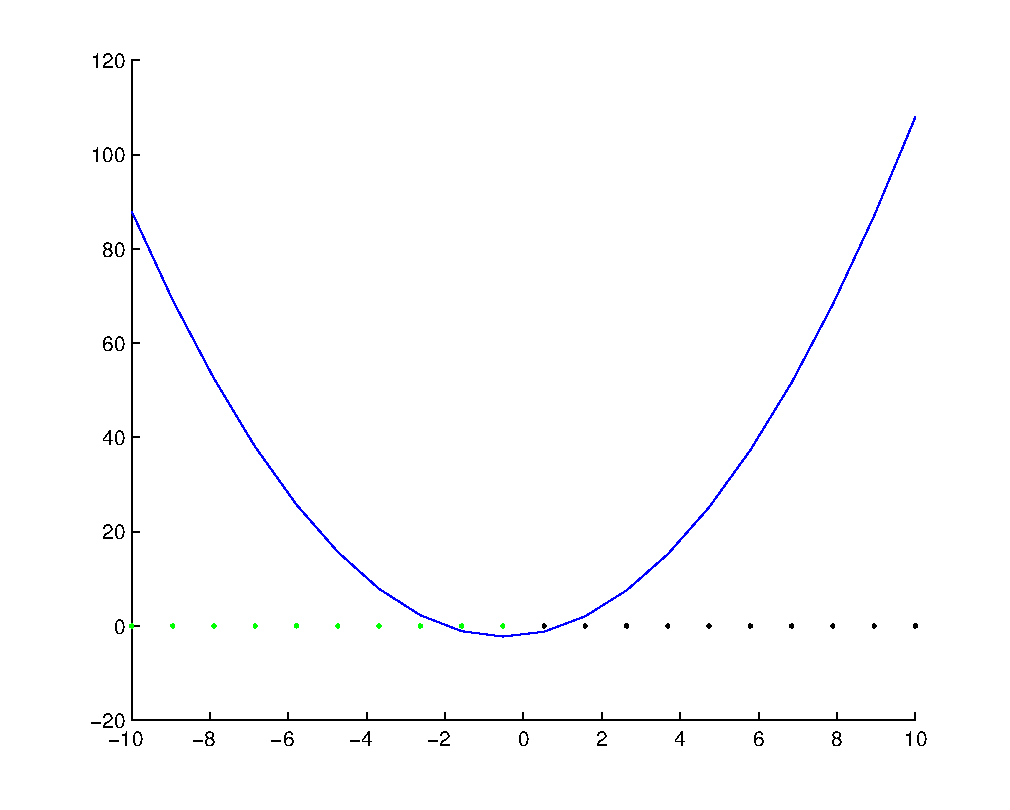
\includegraphics[scale=0.5]{./Figures/basins1}
\caption{The plot of $f(x) = x^2 + x - 2$ along with 20 seed values for Newton's Method.  The green values all converge to the root at -2, and the black values will converge to the root at 1.}
\label{Fig:basins1}
\end{center}
\end{figure}

It turns out that for $f(x) = x^2 + x - 2$, any seed value will converge to one root or the other.  We call the set of points that converge to a single value through an iterative process a basin of attraction.  We can see in Figure \ref{Fig:basins1} a set of seed values that are color coded to indicate which root they converge to with Newton's method.

\begin{problem}
Write a function that will draw a quadratic function with two real roots and then draw/color-code the basins of attraction on the x-axis (as in Figure \ref{Fig:basins1}).  Accept a parameter that determines the number of evenly spaced seed values to try.  This way you can adjust the ``resolution'' of your basins by increasing the number of seed values.
\end{problem}
\begin{problem}
Let $f(x) = x(x-1)(x+1)$.  Predict what the basins of attraction will look like and then plot them.  Is the result what you expected?
\end{problem}

%\begin{itemize}
%\item Quick overview of complex functions.  Maybe make a shout out to analytic = nice?
%\item Definition of orbits of complex functions
%\item attractors/repellers, fixed points etc.
%\item simple definition of julia set
%\item We will be looking at functions that look like $f(z)  = z^2 - c$
%\end{itemize}

We now extend these ideas to complex functions.  There is an entire field of mathematics devoted to the study of such functions, but here we only examine some basic properties as they pertain to the generation of Julia sets.  Like other functions we have thus far been exposed to, a complex function maps an input to a unique output.  However, in this case both the input and the output come from the space of complex numbers.%  We also have a conception of what a ``nice'' function is for real numbers, usually along the lines of continuity.  For complex functions, we have a similar concept of niceness called analyticity.

Given a sufficiently ``nice'' complex function, we can apply Newton's method in a similar way to how we applied it in the real case.  However due to the nature of the space we are mapping from and to, we no longer have access to the intuitive visual representations of functions that we saw in the real case.  We can, however, graph the basins of attraction for Newton's method on the complex plane.  For example, let:
\[
f(z) = z^2 - 1
\]
Derivatives for nice complex functions behave much the same way as in the real case:
\[
f'(z) = 2z
\]
It is straightforward to verify that $f$ has two roots at 1 and -1.

%How about an example on how to graph complex equations?
\begin{problem}
Modify your code from the previous problem to graph the basins of attraction of a function over the complex plane.  Examine the basins of attraction for a quadratic complex function such as $f(z) = z^2 - 2z + 1$.  Keeping in mind the previous problems with real valued functions, what do you expect will happen when you examine a cubic complex polynomial?  Plot the basins of attraction of $f(z) = z^3 - 1$.  What happened?
\end{problem}

The complex behavior on the boundaries of the basins of attraction of the cubic polynomial $f(z) = z^3 - 1$ is called a fractal.  This complex and beautiful behavior occurs due to a result from complex analysis that says that the basins of attraction of the Newton map must share a common boundary.  For a linear or quadratic function, this results in boring expected behavior, but when we examine a polynomial of degree 3 or higher we see the complex boundaries arise.  These complex boundaries are called the Julia set of a function (The boring parts of the picture are called the Fatou set).  The interested reader can find more at CITATION NEEDED. Fractal behavior lies at the heart of what is known as chaos, which will be examined in a later chapter.

To finish this section we examine the Julia sets of an iterated complex map.  In this case, instead of examining the basins of attraction of Newtons method, we will simply iterate on the complex function $f(z) = z^2 + c$ where $c \in \mathbb{C}$.  For example, let $c = 0.4 + 0.3i$ and the choose a seed value $z_0$ and iterate on $f$, i.e.
\[
f_{n+1} = f(f_n)
\]
Where $f_1 = f(z_0)$.  Try $z_0 = 0.5 + 0.1i$ and $z_0 = 5 + 5i$ as seed values.  What happens after several iterations of $f$?

\begin{figure}\label{Fig:julia}
\begin{center}
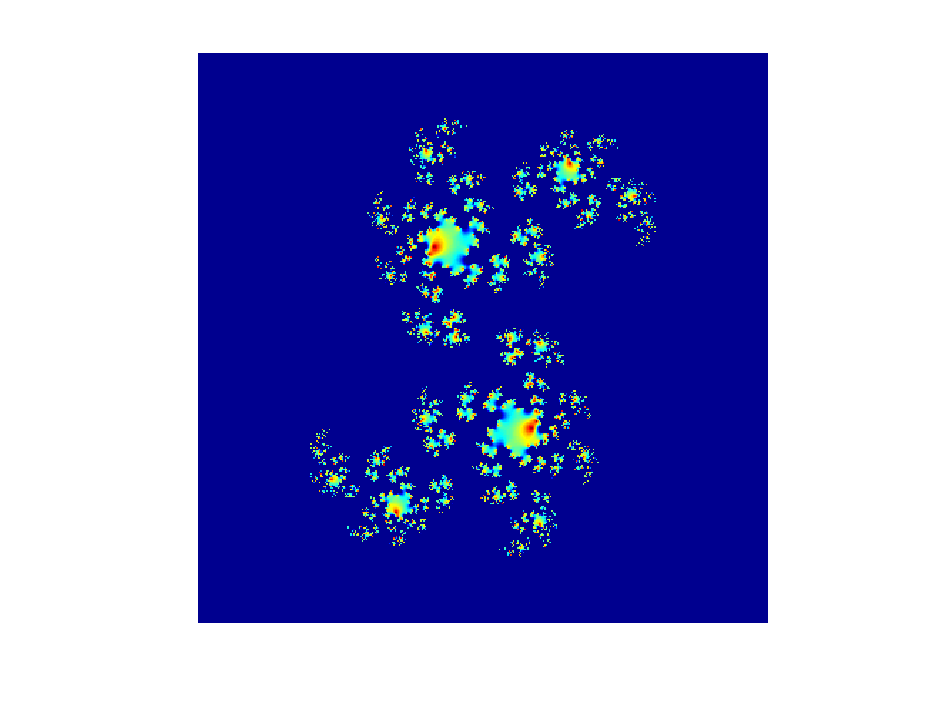
\includegraphics[scale=0.5]{./Figures/julia}
\caption{We let $f(z) = z^2 + 0.4 + 0.3i$ and then iterate on a mesh from $[-1,1]\times[-i,i]$.  The above figure is a plot of $e^{-|z|}$ for each $z$ in the msh after $30$ iterations.}
\end{center}
\end{figure}


\begin{problem}
Generate another grid of complex numbers on $[-1,1]\times[-i,i]$.  Let $f(z) = z^2 + c$ where $c$ is a complex number from the mesh.  Write code that iterates each point in the mesh 30 times, and then plot $e^{-|z|}$ on the resulting mesh.  Try for several values of $c$.  You may want to use the {\tt imagesc} command for plotting your results.
\end{problem}




%Needs to be translated (RDG)

\lab{Applications}{Orthogonal Polynomials}{Orthogonal Polynomials}
\label{OrthoPoly}

\objective{Teach about orthogonal functions, and applications of function spaces.}

Up to this point, our discussion of inner product spaces has primarily focused on $\mathbb{R}^{n}$ and $\mathbb{C}^{n}$. In these cases the power of the inner product is generally already encoded in the structure that we study in elementary linear algebra. However, inner products are much more useful in the context of infinite vector spaces, specifically in studying spaces of functions.

Consider the following inner product:

\[
<f,g> = \int_{-1}^1 f(x) g(x) w(x) dx
\]

This is known as a weighted inner product (w(x) is known as a weighting function). This inner product is over the space $L^2([-1,1])$. We can consider other intervals of integration as desired.

Recall that we call two vectors orthogonal if $<x,y> = 0$. Using this definition we can find functions that are orthogonal.

\begin{example}
The sequence of functions
\[
1,sin(x),cos(x),sin(2x),cos(2x)
\]
is an orthogonal set on $L^2([-\pi,\pi])$, when $w(x) = 1$. This is clear by integrating using the following identities:
\begin{align*}
2 cos(nx)cos(mx) &= cos(n+m)x + cos(n-m)x \\
2 sin(nx)sin(mx) &= cos(n-m)x - cos(n+m)x \\
2 cos(nx)sin(mx) &= sin(n+m)x - sin(n-m)x
\end{align*}

The fact that these functions are orthogonal is crucial in proving that we can approximate any continuous function arbitrarily well using the fourier transform.
\end{example}

\begin{problem}
The gram-schmidt process can be used to transform a linearly independent set $y_k$ into an orthonormal set $x_k$. The process is defined inductively by:

\[
w_1 = y_1
w_k = y_k - \sum_{n=1}^{k-1} <y_k,x_n>x_n, x_k = \frac{w_k}{\norm{w_k}}
\]

Using $w(x) = 1$, apply the gram-schmidt process to the set of polynomials $t^n$. Find the terms for $n \leq 4$. This set of orthogonal polynomials is known as the Legendre Polynomials.
\end{problem}
\begin{problem}
Prove that the Chebyshev Polynomials form an orthogonal set when $w(x) = \frac{1}{\sqrt{1-x^2}}$. Hint: Use the cosine definition and use the change of variables $x = cos(u)$.
\end{problem}

There are several canonical sets of polynomials that are found using this process. Each is based upon a different weighing function. Some examples include the Hermite polynomials and the Laguerre Polynomials.

One useful application of orthogonal polynomials is that it allows us to easily approximate functions.

\begin{problem}
Find a,b,c that minimize
\[
\int_{-1}^1 |x^3-ax^2-bx-c| dx
\]
Hint: In the framework of calculus this problem would be fairly difficult. However, in the framework of inner product spaces this is much less difficult. We are simply projecting $ax^2-bx-c$ onto $x^3$. You can even reuse the calculations you made in finding the Legendre polynomials.
\end{problem}

\lab{Applications}{Markov Chains and Graph Theory}{Markov Chains and Graph Theory}
\label{Markov}

\objective{This section teaches about two simple applications of Linear Algebra. First it teaches about Markov Chains, which in this context represent discrete random transitions. Second it teaches about Graph Theory, which can be used to represent many physical problems.}

\section*{Markov Chains}

%Lab \ref{Markov}

A Markov Chain describe a particular type of random variable. This type of random variable is characterized by the fact that all relevant information is related to its current state. We can easily model this type of random variable using matrices. We will start with a canonical example of a frog jumping from one lilypad to another.

Fredo the Frog hops around between the three lily pads $A$, $B$, and $C$.  If he's on lily pad $A$ and jumps, there is a 25\% chance that he will land back on lily pad $A$, a 25\% chance that he will land on lily pad $B$, and a 50\% chance that he will land on lily pad $C$.  In Figure `2.1, we have a transition diagram that reflects the various probabilities from which Fredo will go from one lily pad to another.

\begin{figure}[h!]
\label{markov1_fig1}
\begin{center}
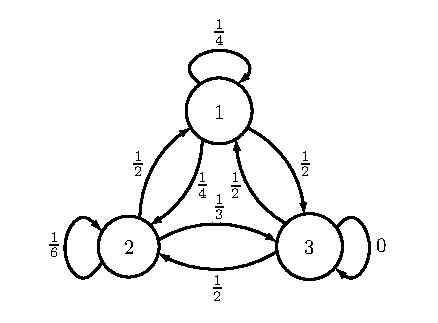
\includegraphics[scale = 1]{./Figures/markov1}
\end{center}
\caption{Transition diagram for Fredo the Frog}
\end{figure}

We can convert our transition diagram into a transition matrix, where the $(i,j)$-entry of the matrix corresponds to the probability that Fredo jumps from the $j^{th}$ lily pad to the $i^{th}$ lily pad (where of course $A$ is the first lily pad, $B$ is the second, and so on).  In Fredo's case, the transition matrix is
\[
A = \begin{pmatrix}
1/4 & 1/2 & 1/2\\
1/4 & 1/6 & 1/2\\
1/2 & 1/3 & 0
\end{pmatrix}
\]
Note that all of the columns add up to one.  This is important.

If Fredo is on lily pad $A$, where will he be after two jumps?  By multiplying the matrix $A$ by itself, we have (approximately)

\[
A^2 = \begin{pmatrix}
0.4375 & 0.3750 & 0.3750\\
0.3542 & 0.3194 & 0.2083\\
0.2083 & 0.3056 & 0.4167
\end{pmatrix}
\]
From this, we infer that there is a 43.75\% chance he will still be on lily pad $A$ after two jumps.  Note that he might have jumped from $A$ to $A$ to $A$, denoted $A \rightarrow A \rightarrow A$, or he could have jumped to one of the other lily pads and then back again, that is, either $A \rightarrow B \rightarrow A$ or $A \rightarrow C \rightarrow A$.  In addition, there is a 35.42\% chance he will be on lily pad $B$ and a 20.83\% chance that he will be on lily pad $C$.  Using \ProgrammingLanguage, we can type in our transition matrix and see where Fredo will be after 5, 10, 20 or 100 jumps.

\begin{matlab}
\begin{lstlisting}[style=matlab]
>> A = [1/4 1/2 1/2;1/4 1/6 1/2;1/2 1/3 0]
>> A^5
>> A^10
>> A^20
>> A^100
\end{lstlisting}
\end{matlab}

\begin{python}
\begin{lstlisting}[style=python]
#Remember, the 1.'s in the numerator force floating point division
: A = sp.array([[1./4,1./2,1./2],[1./4,1./6,1./2],[1./2,1./3,0]])
: np.linalg.matrix_power(A,5)
: np.linalg.matrix_power(A,10)
: np.linalg.matrix_power(A,20)
: np.linalg.matrix_power(A,100)
\end{lstlisting}
\end{python}
Note that in the limit that the number of jumps goes to infinity, we get
\[
A^\infty = \begin{pmatrix}
0.4 & 0.4 & 0.4\\
0.3 & 0.3 & 0.3\\
0.3 & 0.3 & 0.3
\end{pmatrix}
\]
This means that after several jumps, the probability that we will find Fredo on a given lily pad will have nothing to do with where he started initially.
 
\section*{Markov Chains}

We can generalize this notion beyond that of frogs and lily pads.  Let the state of our system be represented by a probability vector
\[
\x = \begin{bmatrix}
x_1\\
x_2\\
\vdots\\
x_n
\end{bmatrix}
\]
where each entry represents the probability of being in that state.  Note that each entry is nonnegative and the sum of all the entries adds up to one.  For example, in the case of Fredo, if we know initially that he is on lily pad $A$, then we have the state vector
\[
\x_0 = \begin{bmatrix}
1\\
0\\
0
\end{bmatrix}
\]
because we know for certainty (100\%) that Fredo is in the first state.  After one jump, we have
\[
\x_1 = A \x_0 = \begin{bmatrix}
0.25\\
0.25\\
0.50
\end{bmatrix}
\]
After two jumps, we have
\[
\x_2 = A \x_1 = A^2 \x_0 = \begin{bmatrix}
0.4375\\
0.3542\\
0.2083
\end{bmatrix}
\]
After a large number of jumps $(n>>1)$, we have
\[
\x_n = A \x_{n-1} = \dots = A^n \x_0 \approx \begin{bmatrix}
0.4\\
0.3\\
0.3
\end{bmatrix}
\]
Since all of the columns are the same for $A^\infty$, then for any initial probability vector $\x_0$, we get the same limiting output, or in other words, all initial vectors converge to the same point, call it $\x_\infty$.  Moreover, we have that
\[
\x_\infty = A \x_\infty
\]
This is called a stable fixed point.  How can we check that a stable fixed point exists?  Hint: Think eigenvalues and eigenvectors.

\section*{Example}

Consider the Markov chain given by
\[
A = \begin{pmatrix}
0.5 & 0.3 & 0.4\\
0.2 & 0.2 & 0.3\\
0.3 & 0.5 & 0.3
\end{pmatrix}.
\]
We show that it has a stable fixed point by checking that it has a single eigenvalue $\lambda=1$.  We do this via Python:
\begin{matlab}
\begin{lstlisting}[style=matlab]
\begin{verbatim}
>> A = [.5 .3 .4; .2 .2 .3;.3 .5 .3]
>> [R, D] = eig(A)
\end{lstlisting}
\end{matlab}
\begin{python}
\begin{lstlisting}[style=python]
: A = sp.array([[.5,.3,.4],[.2,.2,.3],[.3,.5,.3]])
: V = la.eig(A)[1]
\end{lstlisting}
\end{python}
Note that the entries in the $\lambda=1$ eigenvector do not generally add up to one.  Indeed, any multiple of an eigenvector is an eigenvector.  So we need to multiply it by the appropriate constant so that all of the entries add up to one.
\begin{matlab}
\begin{lstlisting}[style=matlab]
>> x = R(:,1)
>> x = x/sum(x)
\end{lstlisting}
\end{matlab}
\begin{python}
\begin{lstlisting}[style=python]
: x = V[:,0]
: x = x/sp.sum(x);x
array([ 0.41836735,  0.23469388,  0.34693878])
\end{lstlisting}
\end{python}
We can check this answer by taking $A$ to a high exponent, say $A^{100}$.

\section*{Assignment}
\setcounter{problem}{0}
\begin{problem}
Suppose a basketball player's success at shooting free throws can be
described with the following Markov chain
\[
A = \begin{pmatrix}.75&.50\\.25&.50\end{pmatrix}
\]
where the first state corresponds to success and the second state to failure.
\begin{enumerate}
\item If the player makes his first free throw, what is the probability that he also makes his third one?
\item What is the player's average free throw percentage?
\end{enumerate}
\end{problem}

\begin{problem}
Consider the Markov process given by the transition diagram in Figure 2 below:
\begin{enumerate}
\item Find the transition matrix.
\item If the Markov process is in state $A$, initially, find the probability that it is in state $B$ after 2 periods.
\item Find the stable fixed point if it exists.
\end{enumerate}
\end{problem}

\begin{figure}[h!]
\begin{center}
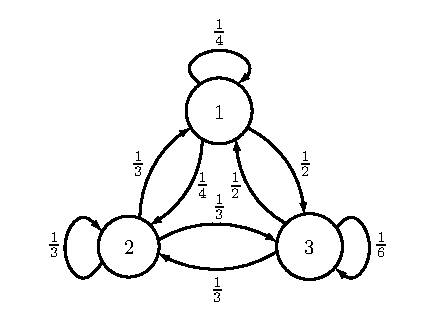
\includegraphics[scale = 1]{./Figures/markov2}
\end{center}
\caption{Transition diagram}
\end{figure}

\newpage

\section*{Graph Theory}
\begin{center}
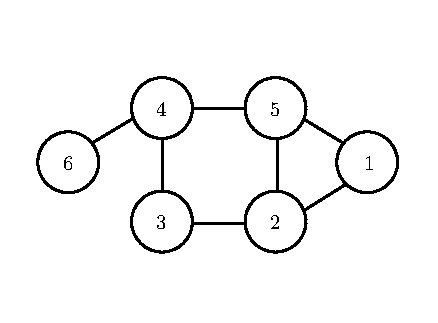
\includegraphics[scale = .8]{./Figures/graphExample}
\end{center}

Graph theory is an important branch of mathematics and computer science. It describes how objects are connected to one another. In a rigorous sense, a graph is composed of two sets: a set of nodes and a set of edges that connect these nodes. 

A graph is directed if connections are uni-directional, and undirected if they are bi-directional. The above graphic shows an undirected graph. We can write a matrix that describes this type of graph. We let each row of our matrix represent our starting point and each column represent our destination. We put a 1 if there is a path and a 0 if there is not. For the above graph we generate the following matrix:

\[
A = \begin{pmatrix}
0 & 1 & 0 & 0 & 1 & 0\\
1 & 0 & 1 & 0 & 1 & 0\\
0 & 1 & 0 & 1 & 0 & 0\\
0 & 0 & 1 & 0 & 1 & 1\\
1 & 1 & 0 & 1 & 0 & 0\\
0 & 0 & 0 & 1 & 0 & 0
\end{pmatrix}
\]

This matrix is called an adjacency matrix. Note that this matrix is symmetric, since the graph is undirected.

What happens if we square an adjacency matrix? It turns out that raising an adjacency matrix to the n power yields the number of paths of length n between two vertices. For example by squaring the above matrix Python gives:
\begin{matlab}
\begin{lstlisting}[style=matlab]
>> A^2
ans =
     2     1     1     1     1     0
     1     3     0     2     1     0
     1     0     2     0     2     1
     1     2     0     3     0     0
     1     1     2     0     3     1
     0     0     1     0     1     1
\end{lstlisting}
\end{matlab}
\begin{python}
\begin{lstlisting}[style=python]
: np.linalg.matrix_power(A,2)
array([[2, 1, 1, 1, 1, 0],
       [1, 3, 0, 2, 1, 0],
       [1, 0, 2, 0, 2, 1],
       [1, 2, 0, 3, 0, 0],
       [1, 1, 2, 0, 3, 1],
       [0, 0, 1, 0, 1, 1]])
\end{lstlisting}
\end{python}

Now try to find the number of connections of length 6 from node 3 to itself. This is simple to do in Python:
\begin{matlab}
\begin{lstlisting}[style=matlab]
>> A^6
ans =
    45    54    38    45    54    16
    54    86    29    77    51    11
    38    29    55    15    70    27
    45    77    15    75    31     4
    54    51    70    31    93    34
    16    11    27     4    34    14
\end{lstlisting}
\end{matlab}
\begin{python}
\begin{lstlisting}[style=python]
: sp.matrix_power(A,6)
array([[45, 54, 38, 45, 54, 16],
       [54, 86, 29, 77, 51, 11],
       [38, 29, 55, 15, 70, 27],
       [45, 77, 15, 75, 31,  4],
       [54, 51, 70, 31, 93, 34],
       [16, 11, 27,  4, 34, 14]])
\end{lstlisting}
\end{python}
It turns out that there are 55 unique paths of length 6 from node 3 to itself. Imagine trying to count all of those paths by hand! It would be very easy to count incorrectly. However, this method makes it very simple to count paths without any mistakes.

The astute reader may ask now why this matters. It turns out that the study of graphs and connectivity have many important applications. For example, connections between web pages can be described as graphs. So can flights between airports or friends on social networking sites. The same ideas are applied frequently in computer chip design and in the preservation of endangered species. We will explore one surprising application to chemistry.

Remeber the \li{bucky} array we explored in chapter one? The graph that this matrix represents is a graph for a geodesic dome, which has structure almost identical to certain types of carbon atoms. Understanding the graphs of certain types of molecules allows scientists to better understand the structure of the molecule, making identification and manipulation easier.

We will manipulate the matrix the \li{bucky} to simulate the types of analysis a scientist could do on a complex carbon atom. For our purposes, each column and row of the \li{bucky} matrix represents an atom in our molecule, and connections are chemical bonds from one atom to another.

\begin{problem}
\begin{matlab}
 Find the number of connections between atoms in our molecule(the command nnz may be useful). Then find the number of atoms that are connected by paths of length two. Three? At what path length are all of the atoms connected?
A nifty way to visualize this is the \li{spy} command. Read the documentation for \li{spy} and then use \li{spy} to visualize how the graph is connected at path length one, two, four and ten.
\end{matlab}
\begin{python}
Find the number of connections between atoms in our molecule(the command \li{sp.count\_nonzero} may be useful). Then find the number of atoms that are connected by paths of length two. Three? At what path length are all of the atoms connected?
A nifty way to visualize this is the \li{plt.spy} command. Read the documentation for \li{plt.spy} and then use \li{plt.spy} to visualize how the graph is connected at path length one, two, four and ten. Remember, to load \li{``bucky.csv''} into an array use the command \lstinline{bucky = sp.loadtxt ( "bucky.csv" , delimiter = "," )}.
\end{python}
\end{problem}


\lab{Applications}{Leontief Input-Output Model}{Input-Output Models}
\label{Leontief}

\objective{Explain the basics of input-output models, and apply them to analyze a state economy.}

One of the core purposes of linear algebra is to model the interactions between a large number of variables in a concise way. We can use this tool to simplify the analysis of very complicated, interactions in a variety of settings.

For example, in economics one might be interested in how one the inputs of one sector of an economy are reliant upon the outputs of another economy. For example, to build a car you need refined steel, plastic, and glass, which are all outputs of other sectors of the economy. Thus if the car industry decides to produce more cars it will accordingly force increased production in several other sectors of the economy, including steel, plastic and glass. This type of interaction is described in economics using what is called the \emph{Leontief Input-Output model}, or just an Input-Output model.

We will explain the basics of this model using a simple imaginary economy involving agriculture, textiles and construction.

Suppose that we have the data given in Table \ref{IORawTable} (we could say that it is in terms of millions or billions of dollars if we wished to make the numbers realistic). In this table the columns represent the inputs to a particular industry and the rows represent outputs. This matrix is known as the exchange matrix. If we divide each column by the output of the corresponding industry we can obtain a coefficient matrix that represents the amount of each input we need to obtain one additional unit of output. This matrix is known as the consumption matrix. We can do this in \ProgrammingLanguage as follows, and we obtain the coefficients in Table \ref{IOCoefTable}.
\begin{python}
\begin{lstlisting}[style=python]
: IO = sp.array([[250,150,30,600],[25,25,20,280],[50,20,5,120]])
: IOCoeff = IO[:,0:3]/sp.dot(sp.ones((3,1),dtype=sp.float_),IO[:,3].reshape(1,3))
\end{lstlisting}
\end{python}

\begin{matlab}
\begin{lstlisting}[style=matlab]
>> IO = [250 150 30 600;25 25 20 280; 50 20 5 120];
>> IOCoeff = IO(:,1:3)./(ones(3,1)*IO(:,4)')
\end{lstlisting}
\end{matlab}
So, for example, to produce one extra unit of agriculture output we need to input .4 units of agriculture, .04 units of textiles and .08 units of construction.

\begin{table}
\begin{center}
\begin{tabular}{|c|c|c|c|c|}
\hline
& Agriculture & Textiles & Construction & Total Output \\ \hline
Agriculture & 250 & 150 & 30 & 600 \\ \hline
Textiles & 25 & 25 & 20 & 280 \\ \hline
Construction & 50 & 20 & 5 & 120 \\ \hline
\end{tabular}
\caption{Raw Input Output Data. Columns represent inputs to an industry, and rows represent outputs.}  \label{IORawTable}
\end{center}
\end{table}

\begin{table}

\begin{center}
\begin{tabular}{|c|c|c|c|} 
\hline
& Agriculture & Textiles & Construction \\ \hline
Agriculture & .4167 & .5357 & .25 \\ \hline
Textiles & .0417 & .0893 & .1667 \\ \hline
Construction & .0833 & .0714 & .0417 \\ \hline
\end{tabular}
\caption{Input Output Coefficients. The columns represent the amount of each product needed to produce one additional unit of output.} \label{IOCoefTable}
\end{center}
\end{table}

Now, we can represent the demand $D$ (``net'' output to consumers) by the following equation:
\[
D = X-CX
\]

Where $X$ is the output vector of our economy (the output of each industry) and $C$ is the coefficient matrix that we just found. Now we can rewrite this as:
\[
D = (I-C)X
\]
Now we have a simple relation between demand and production. We can accordingly use the backslash command to predict how changes in demand will affect overall production.

\begin{problem}
What are the demand levels for the three product economy? This can be solved for either using backslash and the coefficient matrix or by directly using the raw data.
\end{problem}

\begin{problem}
If demand for construction increases by fifty percent what will the output vector of the economy be? This output vector is not readily apparent from the raw data, but can be easily found using the coefficient matrix.
\end{problem}

\begin{problem}
\begin{matlab}
The file \li{WashingtonIOData.txt} contains the raw input output data for the state of Washington in the year 2002. Import the data using the \li{uiimport} command. You can then obtain the raw input output data in the form that we present above using the command: \li{IO = data(1:50,[1:50 60]);}. The source of this file is the file \li{io2002table.xls}, and you can find the industry corresponding to each column using that file.
\end{matlab}
\begin{python}
 %Unknown how to import xls into pylab. Should be simple though, with a bit of tinkering
\end{python}

Find the output vector if the demand for construction increases by ten percent. This will require first finding the initial demand vector, and then increasing the correct entry by ten percent and using backslash to find the new output vector.
\end{problem}

This method can be used to model economies of almost any scale. One of the primary limitations is that this model assumes that production varies linearly in its inputs, which may not be realistic.



\lab{Applications}{PageRank Algorithm}{PageRank Algorithm}
\label{Ch:PageRank}

\objective{Explain the basics of the PageRank Algorithm, and some of its applications}

The PageRank Algorithm is core algorithm used by Google to classify search results. It is based upon an interesting mathematical model that involves random processes, Markov chains and eigenvalues. It ranks pages webpages based upon their connectivity properties with the rest of the web. When you make a query on Google's webpage they find every webpage that contains the keywords you specified and then list them primarily in order of page rank (this isn't true in every case, but it is generally how it works).

The PageRank Algorithm works by supposing that a person surfing the internet randomly clicks links on the webpages. We will notate the probability that the surfer is a particular page $i$ at time $t$ by $PR(i,t)$. We can write an equation for this probability from one time step to the next using the following notation:
\[
PR(i,t+1) = \sum_{j \in M(i)} \frac{PR(j,t)}{L(j)}
\]

Where $M(i)$ is the set of pages that link to page $i$, and $L(j)$ represents the number of outbound links on page $j$. Note that this is simply representing the internet as a markov chain, just like we discussed in Lab \ref{Markov}. We assume that the starting probability is uniform, or in other words that $PR(i,0) = 1/N$.

However, there are two minor modifications that we make to this formula. First, what if a page has no outbound links? In this case we pretend that the page links to every other page (as if the surfer, upon getting stuck, randomly picks a new page). Second, we assume that the surfer sometimes gets bored and randomly picks a new page. The probability that the surfer doesn't get bored is called the damping factor $d$ and is usually set to $.85$. Using these modifications we can write our formula as:
\[
PR(i,t+1) = \frac{1-d}{N} + d\sum_{j \in M(i)} \frac{PR(j,t)}{L(j)}
\]

Note that $N$ is the total number of webpages. We then say that the page rank of a particular webpage is the value
\[
PR(i) = \lim_{t\to \infty} PR(i,t)
\]

Mathematically therefore, the page rank is the steady state probability of our modified Markov chain. We can rewrite this as a matrix equation:
\[
R(t+1) = d K R(t) + \frac{1-d}{N} \begin{pmatrix}1\\\vdots\end{pmatrix}
\]

Where $R_i(t) = PR(i,t)$. The matrix $K$ is defined by:
\[
K_{ij} = \begin{cases} \frac{1}{L(j)} & \mbox{ if j is linked to i} \\ 0 & \mbox{ otherwise} \end{cases}
\]

We can write $K$ neatly as follows:
\[
K = (B^{-1}A)^T
\]

Where $A$ is the adjacency matrix for the directed graph (the edges are links) and $B$ is the diagonal matrix containing the outdegree of each vertex\begin{matlab} (i.e. \li{diag(sum(A'))})\end{matlab}. Recall that we have to modify our graph so that any page without outbound links points to every other page, otherwise these definitions don't make sense (for example $B^{-1}$ will not be well-defined).

There are several ways to solve for $\lim_{t \to \infty} R(t)$. One option is simply iterate the equation until $\norm{R(t)-R(t-1)}$ is sufficiently small. Another option is to instead assume a steady state (i.e. $R(t) = R(t-1)$) giving the equation:
\[
R(t+1) = d K R(t) + \frac{1-d}{N} \begin{pmatrix}1\\\vdots\end{pmatrix}
\]
Which we can then reduce to the following form solvable by least squares:
\[
(I-dK)R = \frac{1-d}{N} \begin{pmatrix}1\\\vdots\end{pmatrix}
\]

A third option is available. Since $R$ can be viewed as a vector of probabilities we can rewrite $\left(\begin{smallmatrix}1\\\vdots\end{smallmatrix}\right) = E R$, where $E$ is a matrix of all ones. Thus the equation becomes:
\[
R = (dK + \frac{1-d}{N}E)R
\]
Since $(dK + \frac{1-d}{N}E)$ will be a strictly positive stochastic matrix (each column sums to one) we can use the Perron-Frobenius theorem to guarantee that this eigenvalue equation corresponds to the largest magnitude eigenvalue and that the eigenvector is unique. Thus by finding the eigenvector corresponding to the largest eigenvalue of $(dK + \frac{1-d}{N}E)$ we can find $R$. This can be found relatively easily using the power method as in lab \ref{Ch:EigSolve}. It actually turns out that the first option for finding $R$ (the iterative approach) is essentially equivalent to the eigenvalue approach.

Once we have calculated $R$ we are done. $R$ gives the page rank associated with each webpage. A useful way to think of this algorithm is to think in terms of voting. Every link that I place on my webpage is a vote for the webpage that it points to. Additionally, if I am more prestigious then my votes count for more.

This algorithm has been used in several settings (primarily in academia). For example, it has been used to rank graduate institutions, to rank impact factor of journals and has even been used in some biological applications.

Let's try implementing the PageRank algorithm on a small subset of the internet. The file \li{internet.dat} contains the connections between webpages on all of the websites supported by Notre Dame University in the year 1999 ({\bf We might need permission to use this file...also need a link}). We can load this data to a sparse matrix using the following:

\begin{matlab}
\begin{lstlisting}[style=matlab]
load internet.dat;
internet(:,1:2) = internet(:,1:2) + 1;
A = spconvert(internet);
\end{lstlisting}

The second line is necessary because the numbering of webpages started at $0$ instead of $1$ in the original data file. The \li{spy} command of this adjacency matrix yields the plot shown in figure \ref{Fig:WebSparse}
\end{matlab}

\begin{python}
\begin{lstlisting}[style=python]
: internet = sp.load("internet.npy")
: A = spconvert(internet)
\end{lstlisting}
The \li{matplotlib.pyplot.spy} command of this adjacency matrix yields the plot shown in figure \ref{Fig:WebSparse}
\end{python}


\begin{figure}
\begin{center}
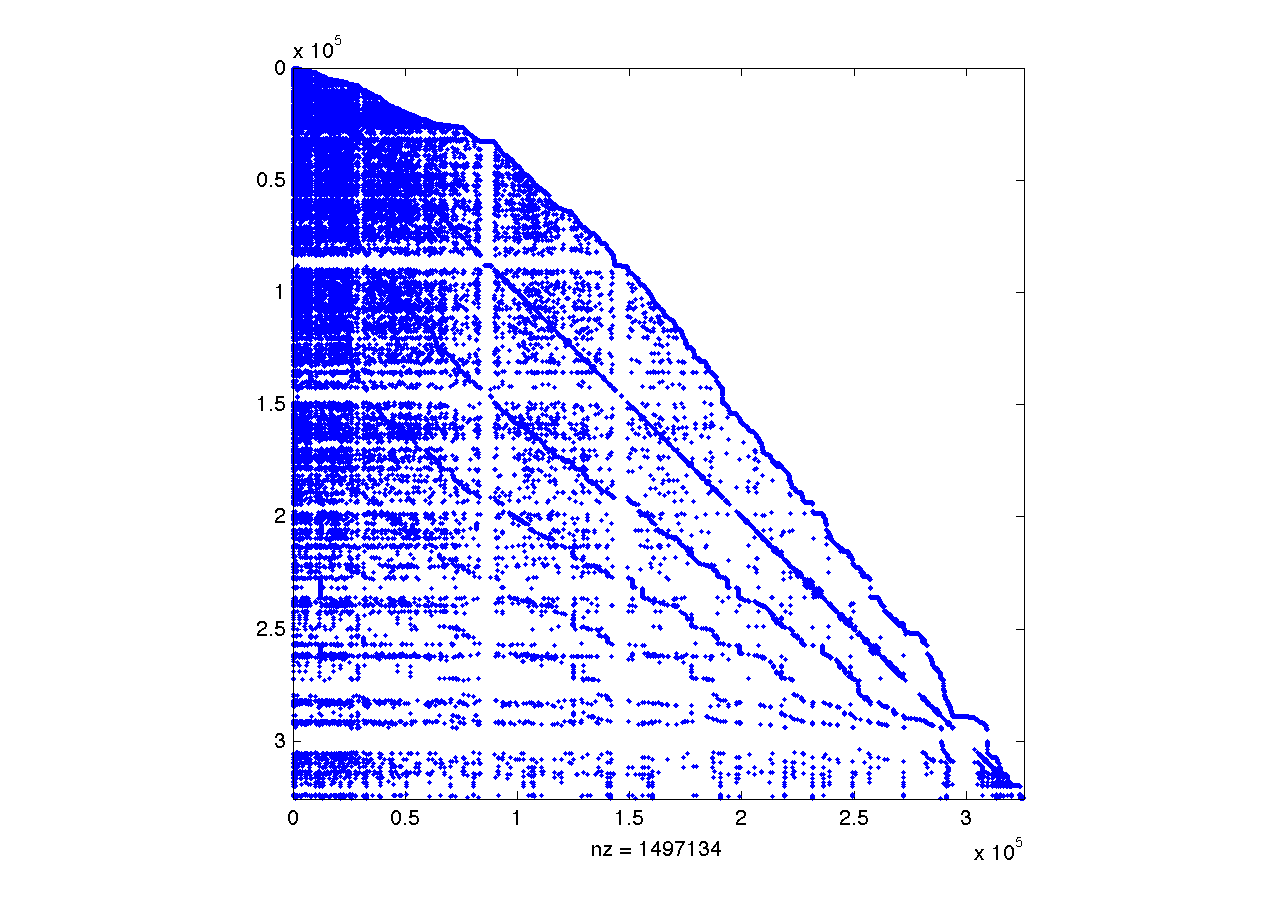
\includegraphics[scale = .4]{./Figures/WebSparse.pdf}
\caption{\li{spy} command on the adjacency matrix corresponding to a portion of the internet}
\label{Fig:WebSparse}
\end{center}
\end{figure}

\begin{problem}
\label{prob:pg_undirected}
A directed graph is called weakly connected if the associated undirected graph (the graph obtained by replacing all directed edges by undirected ones) is connected. Use the eigenvalues of the graph laplacian to determine whether the graph representing this portion of the internet is weakly connected (refer to lab \ref{Ch:EigGraph} if you don't remember how to do this).
\end{problem}

\begin{problem}
\label{prob:pg_calc}
Calculate the PageRank on the first 6000 webpages in the data set. Remember that first you must set any rows that are all zeros to be rows of ones. Which page has the highest page rank, and what is the value of the page rank? Which method works the best? Why?
\end{problem}
%Solution: page number 1, .0643

\begin{problem}
The iterative method allows the easiest implementation for large-scale problems (everything can be done using sparse matrices). Using an implementation that uses only sparse matrices, calculate the PageRank on the entire set of webpages. Which page has the highest page rank, and what is the value of the page rank?
\end{problem}
%Solution: page number 1964, .0055

% Needs to be translated
%Need permission and web address for internet.dat

%==================================================
%End of the first half
%==================================================


%---------------------------------------------------------------
%These labs cover integration and approximation theory. They are combined labs


%These labs still need to be merged/translated

\lab{Algorithms}{Barycentric Lagrange Interpolation}{Barycentric Lagrange Interpolation}
\label{lab:Barycentric}
\objective{This section explains the basic interpolation problem, and how to use Barycentric interpolation to solve the problem.}

\begin{comment}
TODO:
Point out difference between problem conditioning and numerical stability.
Using evenly spaced points as opposed to the chebyshev nodes
\end{comment}

Suppose that we have $n$ distinct points $\{x_n\}$ with associated function values $f(x_i) = y_i$. Which polynomial of degree $n$ matches the function at the specified points? This problem is known as polynomial interpolation. It is important in a variety of fields, including numerical integration(which we will cover in the next few labs).

A polynomial of degree $n$ can be written as

\[
p(x) = a_0 + a_1 x + \ldots + a_n x^n
\]
Now, by collecting our coefficients we can actually reformulate our problem as a matrix equation:
\[
\begin{pmatrix}
1 & x_1 & x_1^2 & \ldots & x_1^n \\
1 & x_2 & x_2^2 & \ldots & x_2^n \\
\vdots & \vdots & \vdots & \ddots & \vdots \\
1 & x_n & x_n^2 & \ldots & x_n^n \\
\end{pmatrix} \begin{pmatrix}
a_0 \\
a_1 \\
\vdots \\
a_n
\end{pmatrix} = \begin{pmatrix} y_1 \\ y_2 \\ \vdots \\ y_n \end{pmatrix}
\]

The matrix on the left of this equation is known as a Vandermonde matrix. It can be proven that Vandermonde matrix will have non-zero determinant if and only if  all of the $x_n$ are distinct. This implies that the equation has a unique solution, or in other words that the polynomial interpolation problem has a unique solution. The command \begin{matlab}\li{vander}\end{matlab}\begin{python}\li{sp.vander}\end{python} creates a flipped version of our Vandermonde matrix (there are several naming conventions, and \begin{matlab}\li{fliplr(vander())}\end{matlab}\begin{python}\li{sp.fliplr(sp.vander())}\end{python} will create the matrix we're talking about).

However, this formulation is not very useful for actually solving for the coefficients $a_i$. This is because the matrix is severally ill-conditioned.

\begin{matlab}
\begin{lstlisting}[style=matlab]
>> cond(vander(1:15))
ans =
   2.5824e+21
\end{lstlisting}
\end{matlab}
\begin{python}
\begin{lstlisting}[style=python]
: import numpy as np
: %To work around hardware limitations we need to use floats in
: %our np.arange.  Otherwise, integer overflow will occur producing
: %incorrect results.
: np.linalg.cond(np.vander(np.arange(1.0,16.0)))
2.5824111670978156e+21
\end{lstlisting}
\end{python}

This is an astronomically large condition number for a $15 \times 15$ matrix. Even if we consider ``nicer'' interpolation points $x_n$ as in the following code, the matrix is still poorly-conditioned (we'll discuss these nicer interpolation points, known as the Chebyshev nodes, later):

\begin{matlab}
\begin{lstlisting}[style=matlab]
>> ind = 1:15;
>> cond(vander(cos((2*ind -1)*pi/30)))
ans =
   1.1900e+05
\end{lstlisting}
\end{matlab}
\begin{python}
\begin{lstlisting}[style=python]
: import scipy as sp
: ind = np.arange(1,16)
: np.linalg.cond(np.vander(np.cos((2*ind-1)*np.pi/30.0)))
118998.85202836856
\end{lstlisting}
\end{python}

We can clearly see that the Vandermonde matrix approach is not a good approach comutationally.

Instead, we take a different approach. Consider the order $n$ polynomial $L_j$ that has the properties:
\[
L_j(x_i) = \begin{cases} 0 &\mbox{ if } i \neq j\\ 1 &\mbox{ if } i =j \\ \end{cases}
\]

We alreadly know that such a polynomial exists and is unique by the arguments above. Furthermore, we can solve our interpolation problem using the data $y_j$ through the following equation:
\[
p(x) = \sum_{j=1}^n y_j L_j(x)
\]

How do we actually calculate the $L_j$? The formula most commonly given in numerical analysis textbooks is
\[
L_j(x) = \frac{\displaystyle\prod_{k=1, k \neq j}^n (x-x_k)}{\displaystyle\prod_{k=1, k \neq j}^n (x_j-x_k)}
\]

These polynomials $(L_j)$ are known as the Lagrange basis functions. Solving the interpolation problem using these basis functions is known as Lagrange Interpolation.

\begin{problem}
Write a function that evaluates the Lagrange Interpolant.  It should accept the $x$ and $y$ values of the desired function, an interval, and the number of interpolation points to use in evaluating the Lagrange Interpolant.  A possible function declaration might be \li{lagrange1(ipt_x, ipt_y, start, end, ipoints)}. Test your function on Runge's function on the interval $[-1,1]$:
\[
f(x) = \frac{1}{1+25x^2}
\]
Because of the behavior of the this type of interpolation, it is highly recommened to use Chebyshev Nodes for your \li{ipt_x} values:
\[
x_i = cos\left(\frac{(2i-1)\pi}{2n}\right), i = 1\ldots n
\]
How many interpolating points can your function handle before it breaks down? Test the temporal complexity of your function (You should get something like $O(n^2)$).
%the function becomes unstable around 661 points
\end{problem}

You should have noticed that the function blew up with sufficiently large $n$. This is due to numerical instability inherent to our formulation of the lagrange basis functions. Also, the $O(n^2)$ runtime is slower than desirable.

We digress for just a moment to explain the choice of interpolation points. Why don't we select interpolation points uniformily? It actually turns out that evenly spaced interpolation points are inherently ill-conditioned. This is since a small error in a value $f_k$ near the middle of the interval of interpolation can cause large errors in the interpolant near the boundaries of the interval.

An illustration might be useful. Consider Runge's function from the previous exercise. I generated Figure \ref{Fig:Runge} using the following code:

\begin{matlab}
\begin{lstlisting}[style=matlab]
ipoints = linspace(-1,1,15);
runge =@(x) 1./(1 + 25*x.^2);
xin = linspace(-1,1,1000);
plot(xin,LInterp1(xin,ipoints,runge(ipoints)),'r');
hold on;
plot(xin,runge(xin));
\end{lstlisting}
\end{matlab}
\begin{python}
\begin{lstlisting}[style=python]
import scipy as sp
import matplotlib.pyplot as plt
ipoints = sp.linspace(-1,1,15)
runge = lambda x: 1.0/(1+25.0*x**2)
xin = sp.linspace(-1,1,1000)
plt.plot(xin,LInterp1(xin,ipoints,runge(ipoints)),'r')
plt.hold(True)
plot(xin, runge(xin))
\end{lstlisting}
\end{python}

As you can see in Figure \ref{Fig:Runge} even for a small number of equally spaced interpolation points the interpolant begins to diverge from the function at the edges of the interval. This is known as \emph{Runge's Phenomenon}.

\begin{figure}
\begin{center}
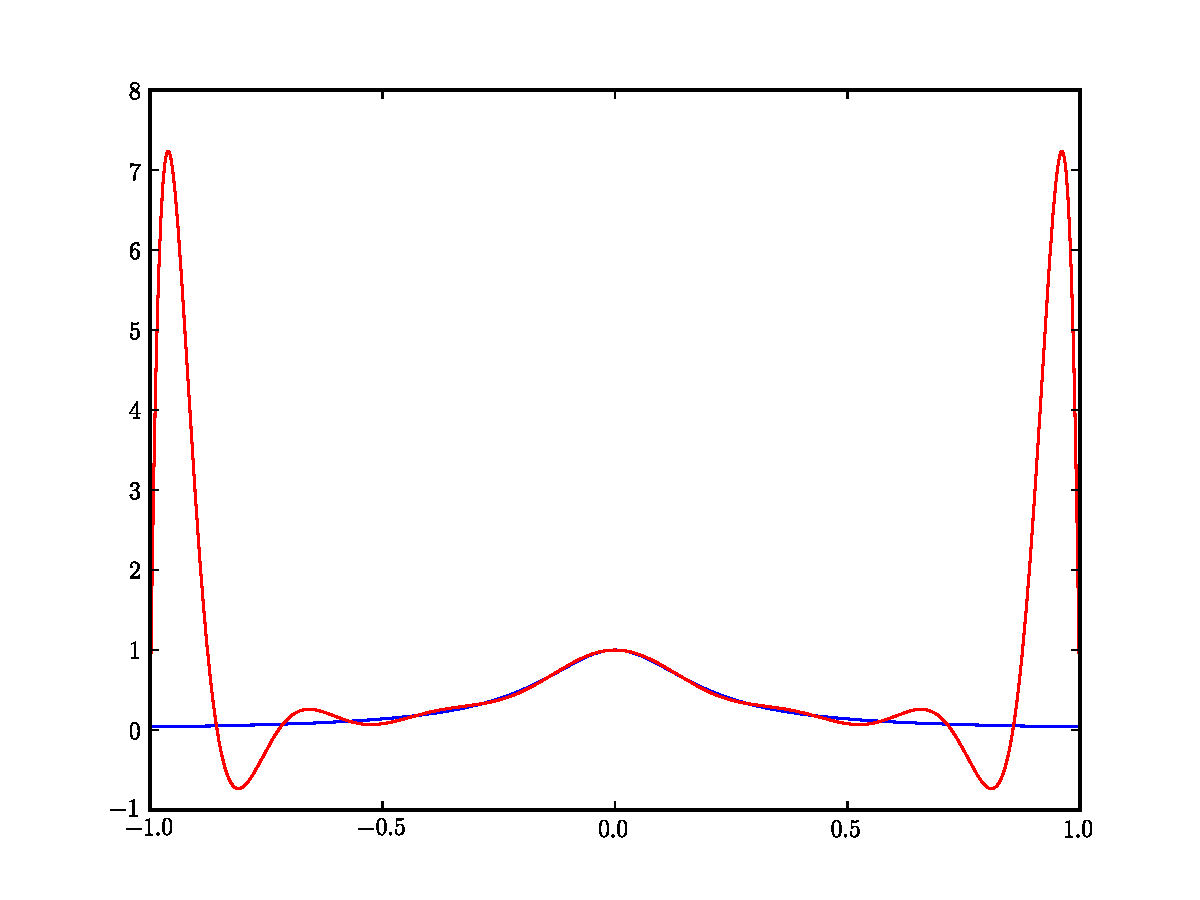
\includegraphics[scale = .5]{./Figures/Runge.pdf}
\caption{An illustration of Runge's Phenomenon, using 15 interpolation points}
\label{Fig:Runge}
\end{center}
\end{figure}


To avoid this phenomenon we must select points that are distributed in a very specific way: with more points on the edge of the interval than the center. The Chebyshev Nodes are one such set of points.

It turns out that we can improve this process greatly by making a few minor modifications. We can rewrite the formulation of our basis functions as follows:
\[
L_j(x) = l(x)\frac{\frac{1}{(x-x_j)}}{\displaystyle\prod_{k=1, k \neq j}^n (x_j-x_k)}
\]

where $l(x) = \prod_{k=1}^n (x-x_k)$. This then allows us to write the interpolating polynomial in the following form:
\[
p(x) = l(x) \sum_{k=1}^n \frac{w_k y_k}{x-x_k}
\]

Where $w_k = \frac{1}{\prod_{k=1, k \neq j}^n (x_j-x_k)}$. This form requires only $O(n)$ computations, a considerable improvment. Furthermore, we note that
\[
1 = l(x) \sum_{k=1}^n \frac{w_k}{x-x_k}
\]

Which allows us to rewrite the interpolating polynomial as:

\[
p(x) = \frac{\displaystyle\sum_{k=1}^n \frac{w_k y_k}{x-x_k}}{\displaystyle\sum_{k=1}^n \frac{w_k}{x-x_k}}
\]

Rewriting the lagrange interpolant in this form is known as \emph{Barycentric Lagrange Interpolation}. This form has the additional advantage that it is numerically stable.

We also note that this formulation makes it clear that we can ignore any factors that are common to the $w_k$ (since they will show up in both the numerator and denominator). This proves critical to the success of our formula (otherwise we will overflow the floating point arithmetic). The easiest way to combat this phenomenon is to multiply each $(x_j-x_k)$ by $C^{-1}$, where $4C$ is the width of the interval on which we are interpolating. This can be done using the following code:

\begin{matlab}
\begin{lstlisting}[style=matlab]
D = max(ipoints)-min(ipoints);
C = D/4;
w = zeros(size(ipoints));
%Calculate Barycentric Weights
shuffle = randperm(length(ipoints)-1);
for k = 1:length(ipoints)
    test = (ipoints(k)-ipoints)/C;
    test(k) = [];
    test = test(shuffle);
    w(k) = 1/prod(test);
end
\end{lstlisting}

Here we use the \li{randperm} function so that the arithmetic doesn't overflow due to poor ordering (if we use the standard ordering we can still get overflow errors because all of the points greater (or less) than one are multiplied together at the same time).
\end{matlab}
\begin{python}
\begin{lstlisting}[style=python]
D = sp.max(ipoints)-sp.min(ipoints)
C = D/4.0
w = sp.zeros_like(ipoints.T)
#Calculate Barycentric Weights
shuffle = sp.random.permutation(len(ipoints)-1)
for k in range(len(ipoints)):
    test = (ipoints[k]-ipoints)/C
    test = sp.delete(test, k)
    test=test[shuffle]
    w[k] = 1.0/sp.prod(test)
\end{lstlisting}

Here we use the \li{sp.random.permutation} function so that the arithmetic doesn't overflow due to poor ordering (if we use the standard ordering we can still get overflow errors because all of the points greater (or less) than one are multiplied together at the same time).
\end{python}

\begin{problem}
Write a new function implementing Barycentric Lagrange Interpolation. Compare runtime with the first function you wrote. Also test how many interpolation points can be handled using this approach (this number should be in the thousands). Use Runge's function again for your tests.
\end{problem}

The Barycentric approach also has other desirable properties (such as easy addition of new points, possible precomputation of weights etc.). It is a powerful, and yet elegant computation tool.%Needs to be translated (RDG)

\lab{Applications}{Monte-Carlo Integration}{Monte-Carlo Integration}

\objective{This section explains the basics of Monte-Carlo Integration.}

Integration is important in a variety of applications. However, high-dimensional integration is highly inefficient using the standard one-dimensional methods. Accordingly, we are forced to pursue a different method. The method of choice in high dimensional settings is known as Monte-Carlo Integration, and is based upon random sampling. This technique is applied in a large variety of fields, such as optimization, physics, and finance.

Consider the following example: Suppose our goal is to estimate the area of a circle (we select this problem because it has a closed form solution, which we can use to test the method). One method that we could use for empirically finding that area is to throw darts randomly at a square board. We then can find the area of the circle by multiplying the square's area by the percentage of darts that fell in the inscribed circle. We can do this using the following code (the resulting figure is shown in Figure \ref{Fig:MCCircle}).

\begin{matlab}
\begin{lstlisting}[style=matlab]
numPoints = 500;
points = rand(numPoints,2);
points = 2*(points-.5);
pointsNorm = hypot(points(:,1),points(:,2));
InCircle = find(pointsNorm < 1);
OutCircle = find(pointsNorm > 1);
plot(points(InCircle,1),points(InCircle,2),'r.');
hold on;
plot(points(OutCircle,1),points(OutCircle,2),'b.');

%Plots a Circle
theta = linspace(0,2*pi,50);
plot(cos(theta),sin(theta),'k');

axis off;
axis equal;

area = 4*length(InCircle)/numPoints;
\end{lstlisting}
\end{matlab}

\begin{python}
\begin{lstlisting}[style=python]
numPoints = 500
points = sp.rand(numPoints,2)
points = 2*(points-.5)
pointsNorm = sp.hypot(points[:,0],points[:,1])
InCircle = sp.nonzero(pointsNorm < 1)
OutCircle = sp.nonzero(pointsNorm > 1)
plt.plot(points[InCircle,0],points[InCircle,1],'r.');
plt.plot(points[OutCircle,0],points[OutCircle,1],'b.');

#Plots a Circle
theta = sp.linspace(0,2*sp.pi,50)
plt.plot(sp.cos(theta),sp.sin(theta),'k')

plt.axis('off');
plt.axis('equal');

plt.show()

area = 4.0*sp.size(InCircle)/numPoints

\end{lstlisting}
\end{python}

\begin{figure}[h!]
\begin{center}
\begin{matlab}
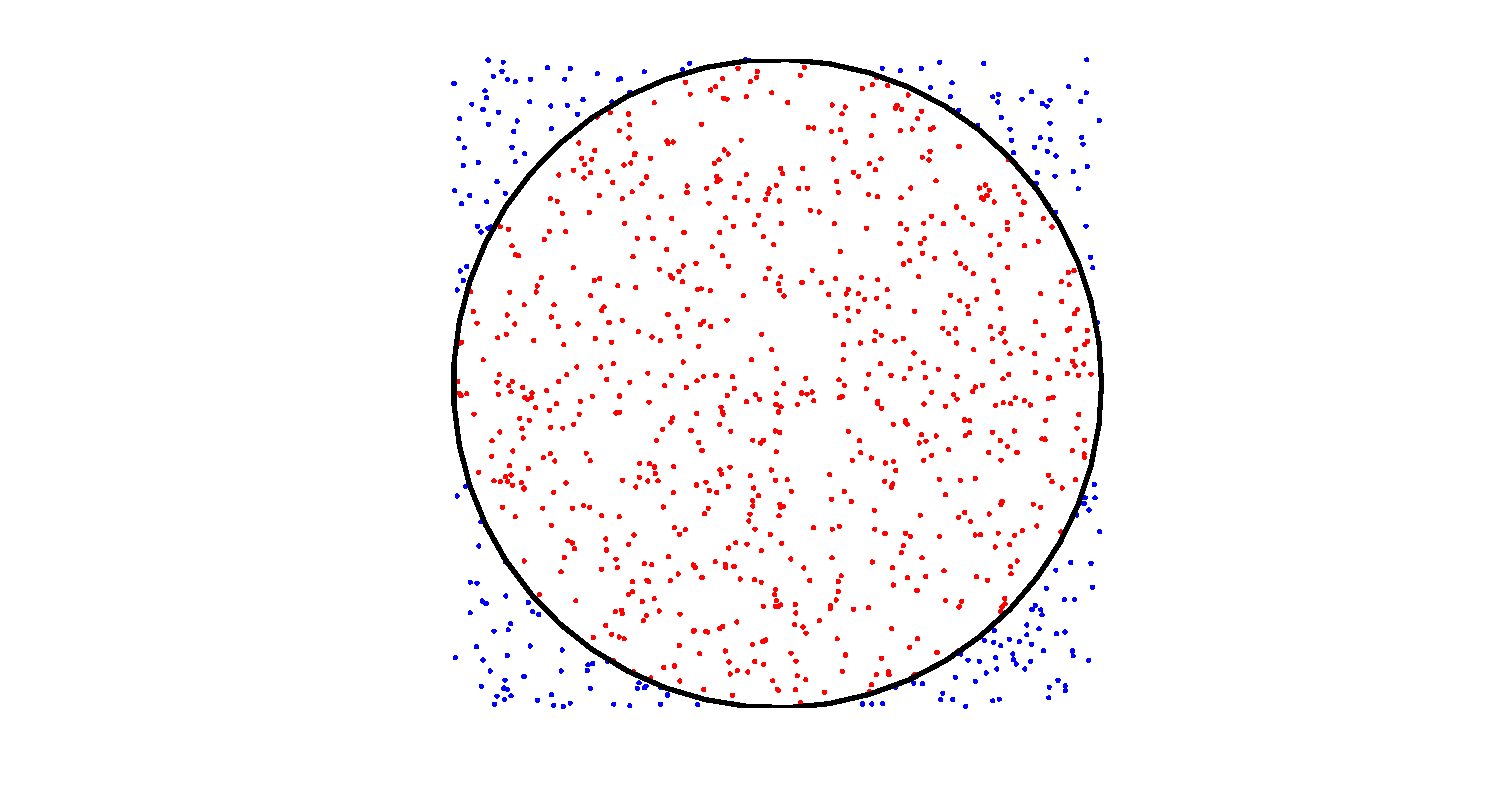
\includegraphics[scale = .4]{./FiguresMAT/MCCircle}
\end{matlab}
\begin{python}
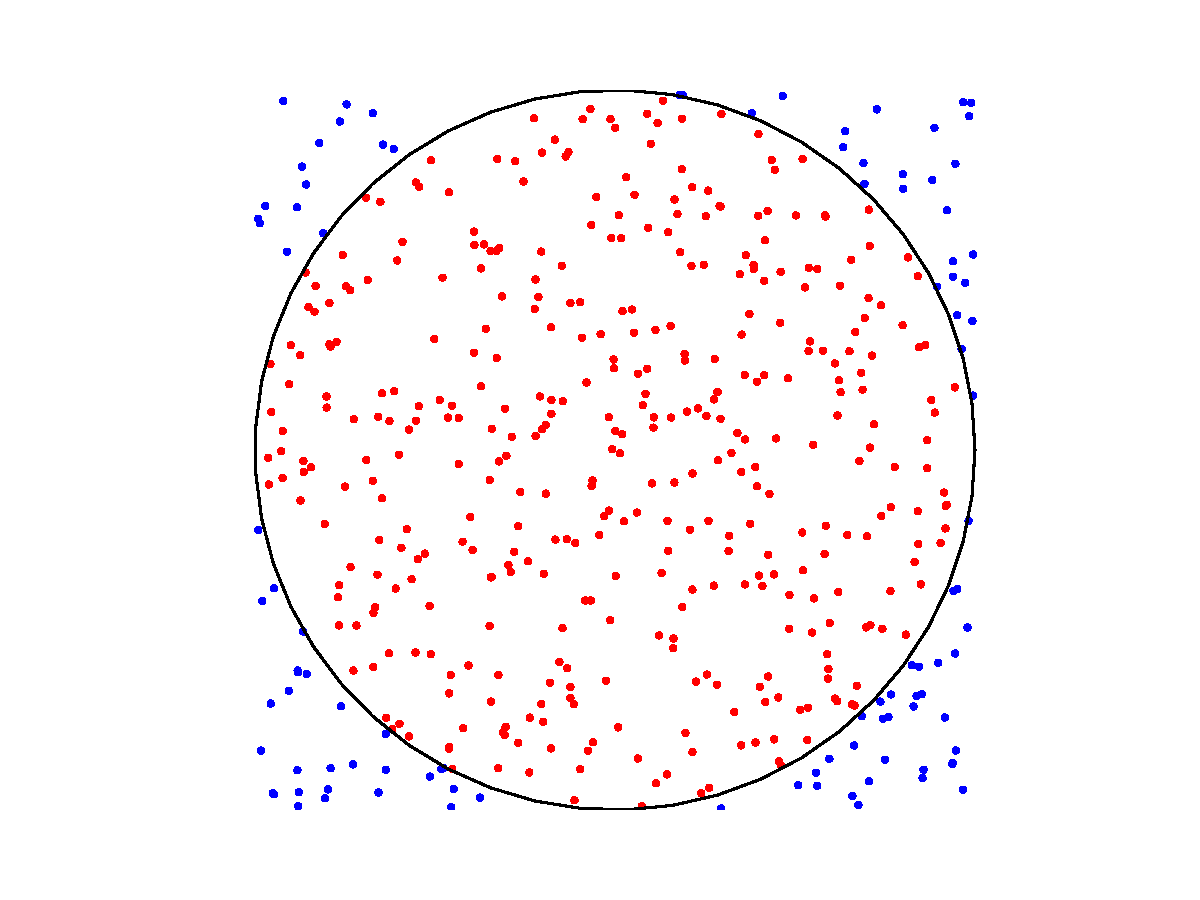
\includegraphics[scale = .4]{./Figures/MCCircle}
\end{python}
\caption{Finding the area of a circle using random points}
\label{Fig:MCCircle}
\end{center}
\end{figure}

In this case the area should be $\pi$, and the approximation is pretty good.

One important question is the rate at which our estimate converges. We can test this using a log plot using the following code:
\begin{matlab}
\begin{lstlisting}[style=matlab]
numTestPoints = 29;
testPoints = round(linspace(1000,100000,numTestPoints));
error = zeros(size(testPoints));
testRuns = 100;
for i = 1:numTestPoints
    for k = 1:testRuns
        numPoints = testPoints(i);
        points = rand(numPoints,2);
        points = 2*(points-.5);
        pointsNorm = hypot(points(:,1),points(:,2));
        InCircle = find(pointsNorm < 1);
        area(k) = 4*length(InCircle)/numPoints;
    end
    error(i) = mean(abs(area-pi));
end
size(error)
size(testPoints)

plot(log(testPoints),log(error))
estimate = [log(testPoints); ones(size(testPoints))]'\log(error');
convergenceRate = estimate(1);
\end{lstlisting}
\end{matlab}

\begin{python}
\begin{lstlisting}[style=python]
numTestPoints = 29;
testPoints=sp.around(sp.linspace(1000,100000,numTestPoints))
error = sp.zeros(sp.size(testPoints))
testRuns=100
area = sp.zeros(testRuns)

for i in range(0,numTestPoints):
	for k in range(0,testRuns):
		numPoints = testPoints[i]
		points = sp.rand(numPoints,2)
		points = 2*(points-.5)
		pointsNorm = sp.hypot(points[:,0],points[:,1])
		inCircle = sp.count_nonzero(pointsNorm < 1)
		area[k] = 4.0*inCircle/numPoints
	error[i] = sp.mean(sp.absolute(area-sp.pi))
sp.size(error)
sp.size(testPoints)

plt.plot(sp.log(testPoints),sp.log(error));
estimate = la.lstsq(sp.vstack((sp.log(testPoints),sp.ones(sp.size(testPoints)))).T,sp.log(error))
convergenceRate = estimate[0][0]
\end{lstlisting}
\end{python}

Note that we estimate the convergence rate using Least Squares, as in Lab \ref{Stats1}. The rate should be something like $-.5$. This means that the estimate of the error improves as $1/\sqrt{N}$, meaning that to improve our error estimate by 10 times (one digit) we must sample 100 times more points. This is not a very desirable convergence rate. However, this rate is independent of the number of dimensions (a property not shared by one-dimensional integration techniques), and is therefore desirable for high-dimensional problems.

The problem of calculating the area of a circle above can actually be reformulated as the following integration problem:
\[
\mbox{Estimate }A = \int_{[-1,1]\times[-1,1]} f(x,y)
\]
where
\[
f(x,y) = \begin{cases} 1 &\mbox{ if $x$ is in the unit circle} \\ 0 &\mbox{ otherwise} \end{cases}
\]

Using a similar method we can actually solve any integration problem. Suppose that we desire to solve the integral
\[
\int_\Omega f(x)
\]

Where $x$ is a vector and $\Omega$ is a region. We can approximate the integral using the formula
\[
\int_\Omega f(x) \approx V(\Omega) \frac{1}{N} \sum_{i=1}^N f(x_i)
\]

Where $x_i$ are uniformily distributed random vectors in $\Omega$, and $V$ gives the volume of a region. This formula exactly describes how to perform Monte Carlo Integration.

\begin{problem}
\label{prob:mc}
Write code implementing Monte Carlo Integration on the unit square for an arbitrary input function. You may require that the user input the number of dimensions. Allow the user to input the number of points to use as well.
\end{problem}

\begin{problem}
\label{prob:mc_test}
Test your solution to Problem \ref{prob:mc}, and the convergence of the method, on the function:
\[
f(w,x,y,z) = sin(x) y^5 -y^3 + zw + yz^3
\]
This integral should converge to zero. Estimate the exponent of convergence (it should be close to $-.5$)
\end{problem}

We note that we must use caution in using monte carlo integration when we don't know if the integral actually converges to a finite value. For example the following integral does not converge(is not finite):
\[
\int_0^1 \frac{1}{x}
\]

We can attempt Monte Carlo Integration on such an integrand using the following code:
\begin{matlab}
\begin{lstlisting}[style=matlab]
k = 5000;
mean(1./rand(k,1))
\end{lstlisting}
\end{matlab}
\begin{python}
\begin{lstlisting}[style=python]
k = 5000
sp.mean(1/sp.rand(k,1))
\end{lstlisting}
\end{python}

We will get a finite value in return, so we could assume (incorrectly) that this integral has a finite value. However, by experimenting with larger values of $k$ you will notice that the integral does not converge to a specific value, which is because the actual integral does not converge. Therefore it is often important to understand some of the properties of the integrand analytically prior to using this type of integration.

Another important key to successful Monte Carlo integration are that the random numbers be uniformily distributed. If they are not, our answer will not converge to a correct answer. This is one of the reason that good pseudo-random number generators are so important.

\begin{problem}
\label{prob:mc_flawed}
Create a new function (based upon the function from Problem \ref{prob:mc}) that uses a ``flawed'' random number generator that doesn't produce numbers between $-.95$ and $-1$. Test your method on the function from Problem \ref{prob:mc_test}. How bad is the error? 
\end{problem}




%
%{\bf Outline:}
%
%\begin{itemize}
%\item Background: High Dimensional Integration is hard. Standard methods can have a hard time focusing on important areas. As we add dimensions we have to sample a lot more points (it adds an order of difficulty)
%\item Toy Example: Area of a shape? Throwing Darts...
%\item Demonstrate how the error decreases ($1/\sqrt{N}$).
%\item Talk about adaptive methods? Give example of how to do this in 1D. This will touch on Approximation Theory. Probably better in the Variance Reduction section.
%\end{itemize}
%
%\begin{problem}
%Calculate a simple 1D problem (maybe using the code for simple newton-cotes from earlier?). Compare convergence with {\tt quad}. Quantify advantages(keep using old data easily). Plot error.
%\end{problem}
%
%\begin{problem}
%Use MC integration to calculate a higher dimensional integral. Maybe a random many-D high order polynomial, or a function we know should go to zero (high order odd function?)
%\end{problem}
%
%{\bf Other possible options (more material/problems)}
%
%\begin{problem}
%Explain Asian Options briefly. Show how to calculate their value using MC techniques.
%\end{problem}
%
%\begin{problem}
%Buffoon's Needle (A simple empirical way to calculate $\pi$) can be formulated as a Monte-Carlo Integration problem. This could be a simulated/experiment lab.
%\end{problem}
%
%\begin{problem}
%Demonstrate need for good ``random'' variables for MC integration to work (maybe use a delibarately flawed prng on the high-dimensional problem above). One more recent test developed for random variables is based on picking subspaces and testing randomness (I think this is in Knuth), we can talk about how this type of flaw applies to MC integration.
%\end{problem}
% (FWG)

\lab{Algorithms}{Newton-Cotes Integration}{Newton-Cotes Integration}

\objective{Explain Newton-Cotes Integration}

One of the fundamental problems in calculus is integration. However, in the vast majority of cases it is impossible to integrate functions analytically. In these cases our only option is to approximate the integral numerically.

One of the most natural approaches is to use the trapezoidal rule. This approach approximates the integral of a function by using the average of its values at the left and right endpoints of the interval of integration:
\[
\int_a^b f(x) dx \approx (b-a)\frac{f(a) + f(b)}{2}
\]

This approach is equivalent to approximating the integral by integrating the linear interpolant of the function. For an illustration see Figure \ref{Fig:Trapezoidal}

\begin{figure}
\begin{center}
\begin{matlab}
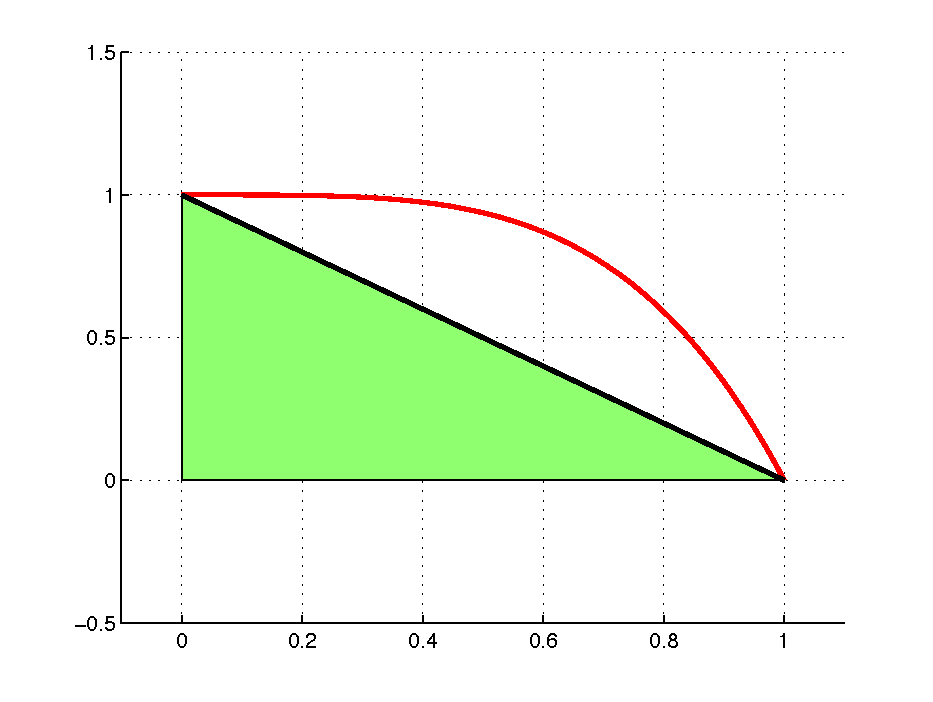
\includegraphics[scale=.4]{./FiguresMAT/Trapezoid.pdf}
\end{matlab}
\begin{python}
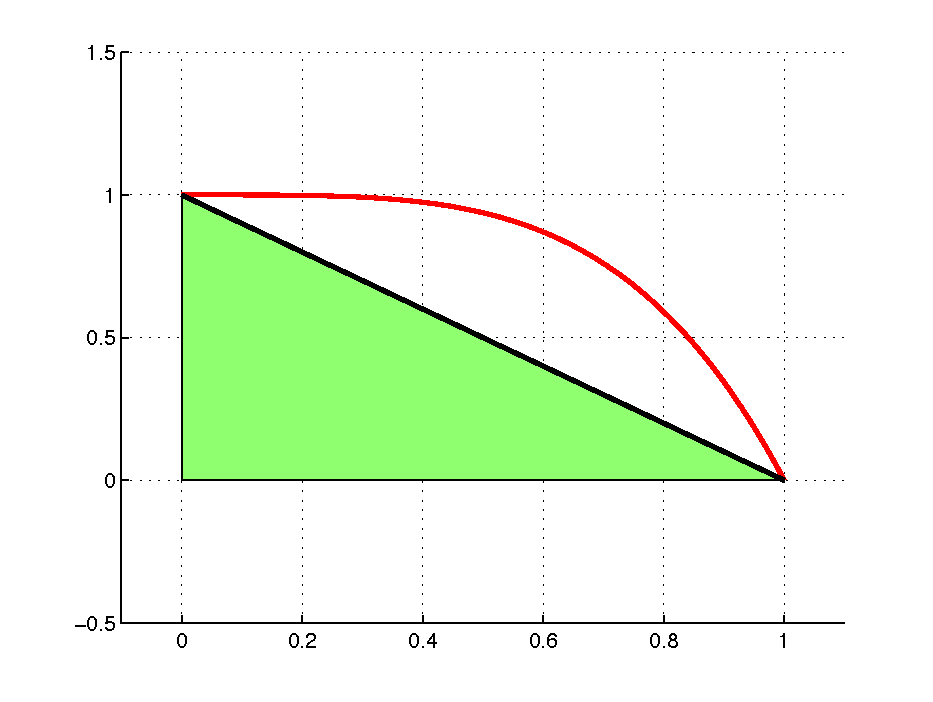
\includegraphics[scale=.4]{./FiguresMAT/Trapezoid.pdf}
\end{python}
\caption{Demonstration of approximating the integral $\int_0^1 (1-x^4)dx$ using the trapezoidal rule. The shaded area is the area approximated by the trapezoidal rule, and the actual function is given in red.}
\label{Fig:Trapezoidal}
\end{center}
\end{figure}

A few quesions rise naturally about the trapezoidal rule. The first is, how good is our approximation? It turns out, that for a twice differentiable function the error is equal to:
\[
\mbox{error} = \frac{(b-a)^3}{12}f^{(2)}(\xi) \mbox{ where } \xi \in [a,b]
\]
Thus, the error is proportional to both $(b-a)^3$ and the second derivative. The fact that the error is proportional to the value of the second derivative makes sense: the trapezoidal rule cannot compensate for a function having non-zero second derivative.

How can we more accurately approximate the integral of a function? One technique is to break our interval into many smaller sub-intervals. This is known as a \emph{composite rule}. We will delay discussion of composite rules momentarily and discuss a different approach first.

Note that the trapezoidal rule is really just approximating the integral by integrating the linear interpolant of the function. Suppose instead that we approximate our function with a higher-order interpolant. We can write this method mathematically as follows:
\[
\int_a^b f(x) dx \approx \int_a^b \sum_{j=1}^n L_j(x)f(x_j) dx = \sum_{j=1}^n f(x_j)\int_a^b L_j(x) dx
\]

We can analytically precompute the value of $w_j = \int L_j(x)$ for a given set of interpolation points $\{x_j\}$ and thus write our approximation as
\[
\int_a^b f(x) dx \approx \sum_j w_j f(x_j)
\]

A set of points $x_j$ and corresponding weights $w_j$ are known as a \emph{quadrature rule}. In this Lab we will focus on evenly-spaced points $x_j$, and in Lab \ref{Lab:GaussQuad} we will look at other sets of points.

Note that this method will exactly integrate polynomials of order $n-1$ (where $n$ is the number of points). This is because the polynomial interpolant ($\sum L_j f(x_j)$) will exactly match the function $f$.

Using three evenly-spaced points we can (using a little algebra) derive the following integration rule:
\[
\int_a^b f(x) dx \approx \frac{(b-a)}{6}\left(f(x_1) + 4 f(x_2) + f(x_3)\right)
\]

This is known as \emph{Simpson's Rule}. \begin{matlab} This is the quadrature rule used in the \li{quad} function in MATLAB.\end{matlab} We can implement Simpson's rule in \ProgrammingLanguage as follows:
\begin{matlab}
\begin{lstlisting}[style=matlab]
function out = SimpsonsRule(fun,a,b)
out = ((b-a)/6)*[1 4 1]*fun([a;(b-a)/2;b]);
\end{lstlisting}
\end{matlab}

\begin{python}
\begin{lstlisting}[style=python]
: def SimpsonsRule(func, a, b):
....: return ((b-a)/6.0)*sp.array([1,4,1])*func(sp.vstack([a,(b-a)/2.0,b]))
\end{lstlisting}
\end{python}


We can test this function on $\sin(x)$ as follows:
\begin{matlab}
\begin{lstlisting}[style=matlab]
>> SimpsonsRule(@sin,0,pi)
ans =
    2.0944
\end{lstlisting}
\end{matlab}

\begin{python}
\begin{lstlisting}[style=python]
: import scipy as sp
: SimpsonsRule(sp.sin, 0, sp.pi)
array([[  0.00000000e+00,   0.00000000e+00,   0.00000000e+00],
       [  5.23598776e-01,   2.09439510e+00,   5.23598776e-01],
       [  6.41202387e-17,   2.56480955e-16,   6.41202387e-17]])
\end{lstlisting}
\end{python}


The answer, which we can find analytically, is $2$. For only evaluating the function at three points this is fairly accurate.

\begin{problem}
Two higher-order quadrature rules are the Simpson 3/8 rule and Boole's rule. They can be written in the following formulae:
\begin{align*}
\int_a^b f(x) dx &\approx \frac{(b-a)}{8}\left(f(x_1) + 3 f(x_2) + 3 f(x_3) + f(x_4)\right) \\
\int_a^b f(x) dx &\approx \frac{(b-a)}{90}\left(7f(x_1) + 32 f(x_2) + 12 f(x_3) + 32f(x_4) + 7 f(x_5)\right) \\
\end{align*}

Write a function that implements these quadrature rules. Allow the user to optionally specify which quadrature rule to use.
\end{problem}

Another tool of great importance in numerical integration is composite quadrature rules. These rules break up the interval into many smaller sub-intervals. A desired quadrature rule is then applied to each sub-interval, and the results are summed together. Mathematically we can write such an approach as follows:
\[
\int_a^b f(x) dx = \sum_{i=0}^n \int_{x_i}^{x_{i+1}} f(x) dx
\]
where $a = x_0 < x_1 < \ldots < x_n = b$. We then apply some rule (such as simpson's rule, or the trapezoid rule) to each smaller integration problem. A graphical illustration of such an approach is shown in Figure \ref{Fig:TrapezoidalComposite}

\begin{figure}
\begin{center}
\begin{matlab}
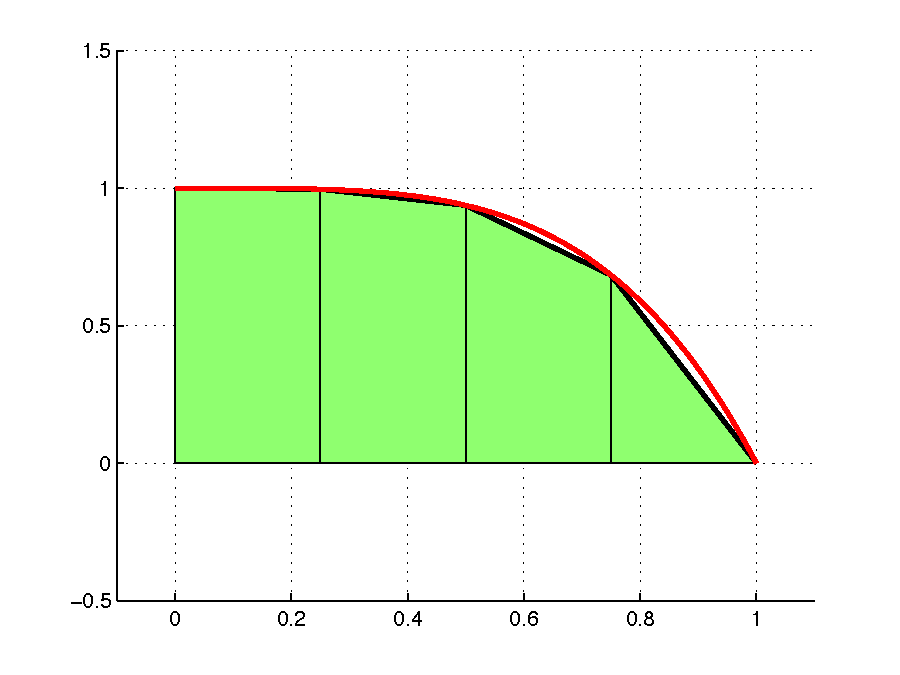
\includegraphics[scale=.4]{./FiguresMAT/TrapezoidComp.pdf}
\end{matlab}
\begin{python}
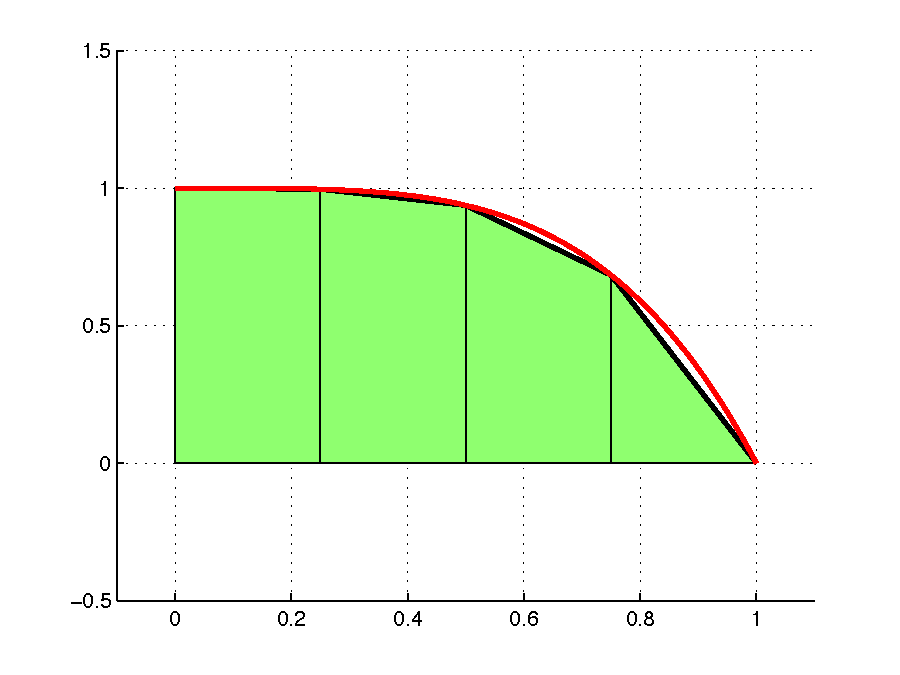
\includegraphics[scale=.4]{./FiguresMAT/TrapezoidComp.pdf}
\end{python}
\caption{Demonstration of approximating the integral $\int_0^1 (1-x^4)dx$ using a composite trapezoidal rule. The shaded area is the area approximated by the composite rule, and the actual function is given in red.}
\label{Fig:TrapezoidalComposite}
\end{center}
\end{figure}

Let's look at how the composite simpson's rule would work. We divide our interval of integration into $n$ sub-intervals (and thus we have $n+1$ interval endpoints). To use Simpson's rule on each sub-interval we will need the $n$ midpoints of each subinterval. Thus we have points $x_1 \ldots x_{2n+1}$. Of these points, the midpoints are precisely the even indices. Now recall that Simpson's Rule is:

\[
\int_a^b f(x) dx \approx \frac{(b-a)}{6}\left(f(x_1) + 4 f(x_2) + f(x_3)\right)
\]

Applying this to each sub-interval we get the following:
\[
\int_a^b f(x) dx \approx \frac{(b-a)}{6n}\left( f(x_1) + \sum_{i=1}^{n} 4*f(x_{2i}) + \sum_{i=0}^{n-2} 2*f(x_{1+2i}) + f(x_{2n+1})\right)
\]

The initial constant is because each sub-interval has width $(b-a)/6n$. The different weights on each function evaluation $f(x_i)$ are justified as follows: each sub-interval midpoint gets weight of four by simpson's rule, and sub-interval endpoints that aren't either $a$ or $b$ get counted twice because they belong to sub-intervals to their left and right.

\begin{problem}
Derive the composite rule for Simpson's 3/8 rule and Boole's rule. Implement all three composite rules in a MATLAB function. Require the user to input a maximum sub-interval width. Now test your function by integrating $x^{1/3}$ on the interval $[0,1]$ (which you can analytically solve). Use a log plot to estimate the exponent of convergence for Simpson's Rule and Simpson's 3/8 Rule. You should get roughly the same exponent of convergence (this does not mean that the errors are the same, just that the rate of convergence is the same). Since the two rules have the same exponent of convergence, but the 3/8 rule requires more function evaluations, the 3/8 rule is typically not used.
\end{problem}

One other important technique is what is known as \emph{Adaptive Quadrature}. It is clear in Figure \ref{Fig:TrapezoidalComposite} that we have approximated the integral better in some places than in others. In fact on the left side of the interval the approximation by linear interpolants is almost indistinguishable from the actual function, while on the right the approximation clearly introduces more significant errors. Adaptive Quadrature methods attempt to identify locations where the error is bad and subdivide only those areas.

One way to approximate the error of a particular integral is to use a composite rule. For example (is we let $S([a,b])$ denote the output of Simpson's rule on a specific interval)

\[
\mbox{Error}(S([a,b])) \approx \abs{S([a,c]) + S([c,b]) - S([a,b])}
\]

Where $c = \frac{b-a}{2}$. We can then decide if the error is appropriately small, and split the interval if it is not. By repeating this process recursively we can acheive the higher accuracy of a very fine composite quadrature rule while only evaluating the function in areas of interest.

This error indicator is very crude, and many other indicators have been proposed. However, they can become complicated relatively quickly, so we won't discuss them here. \begin{matlab} The {\tt quad} function in MATLAB is precisely an adaptive version of Simpson's rule \end{matlab}.

\begin{problem}
Write a function that uses an adaptive version of Simpson's rule. The user should input the maximum error. It should use a recursion. You will have to divide the error between sub-intervals. Have the function output the number of function evaluations required in addition to the value of the integral.

Compare the performance of the this function with the composite rule you wrote earlier on the function $x^{1/3}$ on the interval $[0,1]$. Which runs faster, and how many function evaluations did each require?
\end{problem}
%Needs to be translated
\lab{Applications}{Variance Reduction Techniques}{Variance Reduction Techniques}

\objective{Explain how to apply variance reduction techniques to MC integration}

{\bf Outline:}
\begin{itemize}
\item Intro: Variance Reduction is about improving the variance of estimates of ``simulations''. This technique is used in statistics, system theory, etc. However, here we're just talking about an application to MC integration.
\item Toy example: pick something that varies only in one region, maybe tanh.
\item Explain how uniform sampling is not the most effective way to gather information.
\item Explain a little bit about how sampling correctly minimizes the variance of the error term. Wikipedia has a pretty good explanation in the VEGAS algorithm section. Basically if we pick random variables by the distribution $|f|/I(|f|)$ then we get zero variance in our error estimate.
\item Explain how the VEGAS algorithm tries to do this.
\end{itemize}

\begin{problem}
Estimate integral of $tanh$ using the VEGAS algorithm. Compare with the actual answer. Compare convergence speed with the naive MC integration technique.
\end{problem}

\begin{problem}
Try the VEGAS algorithm on the higher-dimensional problem used in MC integration section. Compare performance.
\end{problem}
%Needs to be written

\lab{Algorithms}{Bezier Curves and B-Splines}{Splines}

\objective{Understand the basics of Bezier Curves, B-Splines and deBoor's Algorithm}

\begin{itemize}
\item Suppose that we wish to smoothly approximate a function. We can't do this with linear interpolants (the derivative is always discontinuous) as we did with tesselation. Here we will investigate a few simple ways to smoothly build curves.
\item One of the difficulties is that we need a method of intuitively manipulating curves (changing tangent values isn't very intuitive). We can use bezier curves because they can b e manipulated intuitively.
\item Explain control points, Bernstein polynomials. Explain that Bernstein polynomials are ill-conditioned.
\item Maybe some extra discussion of the Bernstein polynomials is appropriate here. They allow uniform approximation of any continuous function, but are not useful computationally.
\item Introduce DeBoor's Algorithm (in this context it's called deCasteljau's algorithm). Point out that stability is due to its foundation in convex combinations.
\end{itemize}
\begin{problem}
Implement deCaseljau's algorithm. Investigate speed and stability against known curves, and compare to bernstein basis.
\end{problem}

\begin{problem}
Build an animation showing how the algorithm works. This shouldn't be very hard, but is pretty instructive.
\end{problem}

\begin{problem}
Python: Implement interactive control points.
\end{problem}

\begin{itemize}
\item We can build upon the foundation of bezier curves using a generalization known as b-splines
\item These are essentially piecewise functions, where we guarantee a certain degree of continuity.
\item The central difference is we define knot points, between which the function is a polynomial of specified degree. If we define all of our knots to be at the endpoints of our interval we actually get a bezier curve.
\item Like bezier curves, we have control points, which allow us to manipulate the curve in an intuitive way.
\item Talk about the definition, note, once again, the bernstein polynomials that would make direct evaluation difficult.
\item Talk about DeBoor's algorithm, which allows, again for easy, stable evaluation.
\end{itemize}

\begin{problem}
Extend the problems from bezier curves to allow b spline input and output.
\end{problem}

\begin{problem}
Is there a way to use barycentric langrange interpolation here? Test it out... (more of a curiosity than a problem I guess...)
\end{problem}

\begin{problem}
B Splines cannot represent certain classes of common curves exactly, such as circles. Explain why this is: I don't understand it well, but it's stated in numerous locations. This will help motivate nurbs later.
\end{problem}
%Needs to be written
\lab{Applications}{Surfaces in 3D and Tesselation}{Tesselation}

\objective{Understand the basics of tesselation in 3D}

{\bf Outline:}
\begin{itemize}
\item Intro: In a graphics application, how do you calculate how surfaces look? There are a few options: parametrize the surface (which can be costly) or tesselate the surface (which may reduce quality).
\item Toy Problem: How do we best represent a sphere?
\item Mesh Refinement. Basically we start with an approximation and refine our approximation one step at a time. This allows a natural structure for the information about refinements (they can represent tesselation data in wavelets this way, Tony DeRose did this).
\item In the case of the sphere we do this using a dodecahedron, and then splitting each face into four faces.
\end{itemize}

\begin{problem}
Tesselate the sphere. Observe error associated with each face. In this case the errors will be uniform. Note that the error can be posed as an itegration problem (we can use different quadrature rules)
\end{problem}

\begin{problem}
Tesselate an ellipsoid. Generate an appropriate error estimator, and refine the tesselation adaptively in appropriate areas.
\end{problem}

\begin{problem}
Specular highlights: there is a bright spot corresponding to where the light reflects directly off of of a surface towards a viewer.The amount of specular light that reaches the viewer is based on different types of distributions (``phong'' is the name of the most common). For a tesselated surface this will be easy to calculate (since the surface normal is easy to determine, and there are a finite number of different surface normals), and for a fine tesselation on a surface this could look cool. Ideas: 1)have a moving light, and have the specular light calculated each time the light is moved 2) Give them a more complex tesselated surface, and have them compute the specular highlights. NOTE: this would take a fair bit of additional explanation, it would be cool, but it might be too much for here. We just have to decide a direction.
\end{problem}
%Needs to be written


\lab{Algorithms}{Gaussian Quadrature}{Gaussian Quadrature}
\label{Lab:GaussQuad}
\begin{itemize}
\item In the section on Newton Cotes we saw the difficulty that arises when we use uniformly spaced points (Runge's phenomenon). Can we do better with unevenly spaced points?
\item Explain the gaussian quadrature rule. Explain that it is only appropriate for functions that can be well-approximated by polynomials, and that it is exact for polynomials of sufficiently small degree (not exact in floating point though...)
\item Discuss how we calculate this rule (There's a matrix that we generate, tri-diagonal, of which we need to find the eigenvalues). This is a $O(n^2)$ operation.
\item Explain that the rule as it stands does not allow nesting(and thus adaptive methods), which is crucial. Explain how the Gauss-Konrod rules fix this problem.
\end{itemize}

\begin{problem}
Code up how we find the integration points and the weights.
\end{problem}

\begin{problem}
Code up the actual Gaussian Quadrature method.
\end{problem}

\begin{problem}
This technique can be extended to integrals with other types of weighting functions. Gauss Hermite Quadrature could be interesting to explain and code up, since it involves an infinite domain.
\end{problem}

\begin{problem}
Clenshaw-Curtis quadrature follows a similar approach. Explain that it is based upon finding the roots of the chebyshev polynomial, and deriving the correct weights (which can be done faster than the gaussian quadrature rule). Code and compare performance.
\end{problem}



 
%Needs to be written
\lab{Applications}{Non-uniform Rational B-Spline}{NURBS}

\objective{Understand the basics of Non-uniform rational b-splines.}

{\bf Outline:}

\begin{itemize}
\item Explain some of the limitations of B-Splines (which we discussed previously. This includes lack of continuity of curvature (cubic B-Splines may have discontinuous curvature at knot points). Another major limitation is inability to represent conic sections (such as circles).
\item Explain that making the splines rational gives us greater flexibility, particularly in representing conic sections.
\item Note that these applications are useful in modelling and computer graphics
\item Example: a circle. Note that the curve doesn't travel uniformily around the circle. This makes sense, otherwise we could describe trig functions exactly using a rational function.
\item Note that we can use an adapted form of deBoor's Algorithm
\end{itemize}

\begin{problem}
Code up deBoor's to evaluate NURBS curves. This may generalize an earlier exercise.
\end{problem}

\begin{problem}
Use both NURBS and non-rational B-Splines to approximate an ellipse. How close are the two? Which one is computationally faster? Easier for a user?
\end{problem}

\begin{itemize}
\item Discuss Nurbs surfaces. Explain that much of 3-D modelling is based upon this. The extension for the math is not terribly difficult.
\item Also recall useful properties of B-Splines that are retained in rational form (invariant under affine transformations).
\end{itemize}

\begin{problem}
Create a NURBS sphere. Show how the surface is not parametrized uniformily.
\end{problem}
%Needs to be written

%---------------------------------------------------------------
%This is one lab about more advanced visualization topics. It will be split by language

\begin{matlab}
\lab{Algorithms}{Scientific Visualization}{Scientific Visualization}

\objective{Go over techniques for making publication ready figures and making other pretty things.}

In this lab we will be focusing on producing publication ready figures in MATLAB.  Thus far we have produced many different plots for several applications.  Here we will focus on different ways of presenting those plots so that they are more informative and aesthetically pleasing.

\section{The \li{plot} Command}  Several of the past labs have required the use of the \li{plot} command.  While what we have done so far as been fairly straightforward as far as plotting is concerned, a quick glance at the MATLAB documentation for \li{plot} reveals a plethora of options for changing the output of the plot command.

How we use the \li{plot} command will vary with our application.  Plotting data requires a very different presentation approach than graphing straight lines.  In the sequel we examine several different options.

\begin{table}[h!]
\begin{center}
	\begin{tabular}{|c|c|}
	
	\hline
	
	Usage & Property Options\\
	
	\hline
	
	\li{Color} & \li{yellow, green, blue} etc., or user defined colors \\& given by $[r g b]$, a three element red, green, \\& blue vector.  See documentation for full list. \\
	
	\hline
	
	\li{LineStyle} & \li{-, --, :, -., 'none'} \\
	
	\hline
	
	\li{LineWidth} & Width in points.  $1$ point is $\frac{1}{72}$ inch.  Default is $0.5$ points. \\
	
	\hline
	
	\li{Marker} & \li{+, *, x, .} etc. See documentation for full list. \\
	
	\hline
	\end{tabular}
\end{center}
\caption{Common Plot commands in MATLAB}
\end{table}

For example, if we wanted to plot $f(x) = x^2$, we don't need to extend our typical plotting knowledge much, except maybe we like green better than blue:

\begin{matlab}
\begin{lstlisting}[style=matlab]
>> x = linspace(-1,5,50);
>> plot(x,f(x),'color','green')
\end{lstlisting}
\end{matlab}

See figure 37.1.

\begin{figure}
\begin{center}
\begin{matlab}
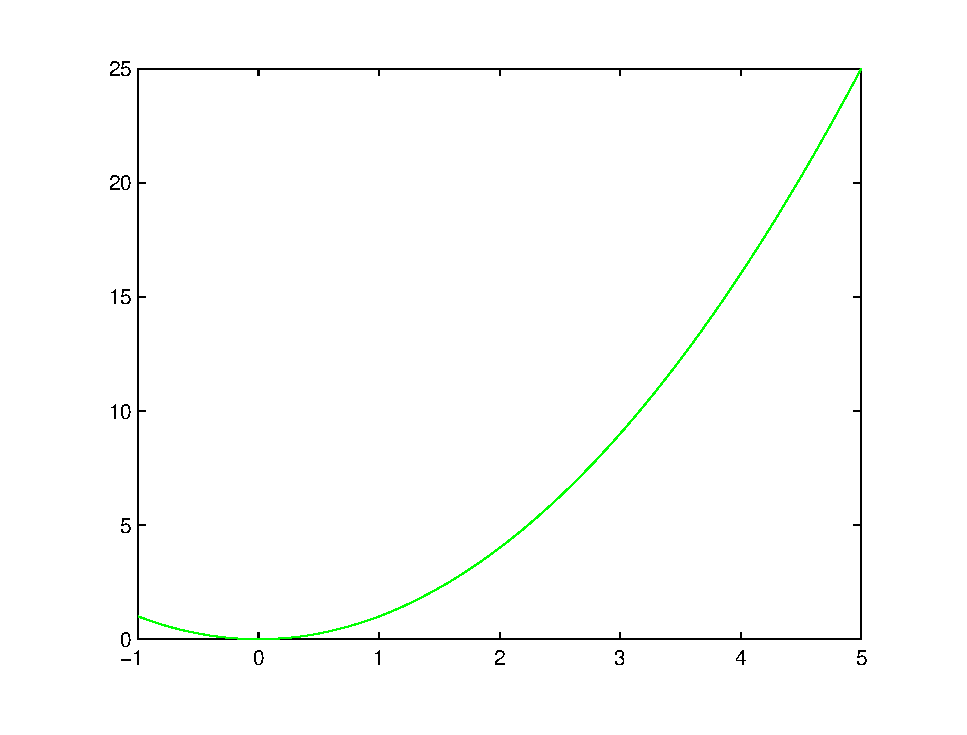
\includegraphics[scale=0.5]{./FiguresMAT/plot1}
\end{matlab}
\caption{Graph of $f(x) = x^2$}
\end{center}
\end{figure}


However, if we wanted to plot the data drawn from a certain distribution, we would want to use the plot command in a very different way.  For example:

\begin{matlab}
\begin{lstlisting}[style=matlab]
>> X = random('Normal',0,1,[100,1]);
>> plot(X,'marker','*','LineStyle','none');
\end{lstlisting}
\end{matlab}

See figure 37.2.

\begin{figure}
\begin{center}
\begin{matlab}
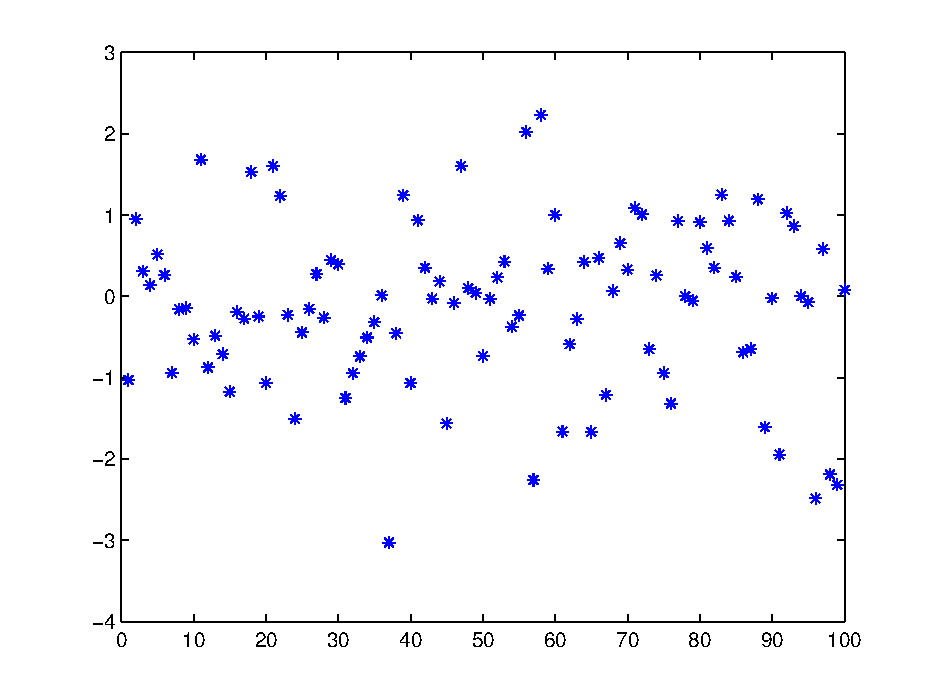
\includegraphics[scale=0.5]{./FiguresMAT/plot3}
\end{matlab}
\caption{100 data points pulled from a normal distribution}
\end{center}
\end{figure}

The \li{hold} command will also be useful for when plotting more than one graph on a single plot.  For example, if we wanted to graph $f(x) = \sin{x}$ and it's derivative $f'(x) = \cos{x}$, we would do the following:

\begin{matlab}
\begin{lstlisting}[style=matlab]
>> f = @(x) sin(x);
>> df = @(x) cos(x);
>> x = linspace(0,2*pi,50);
>> hold on;
>> plot(x,f(x),'color','blue');
>> plot(x,df(x), 'color','green');
>> hold off;
\end{lstlisting}
\end{matlab}

See figure 37.3.

\begin{figure}
\begin{center}
\begin{matlab}
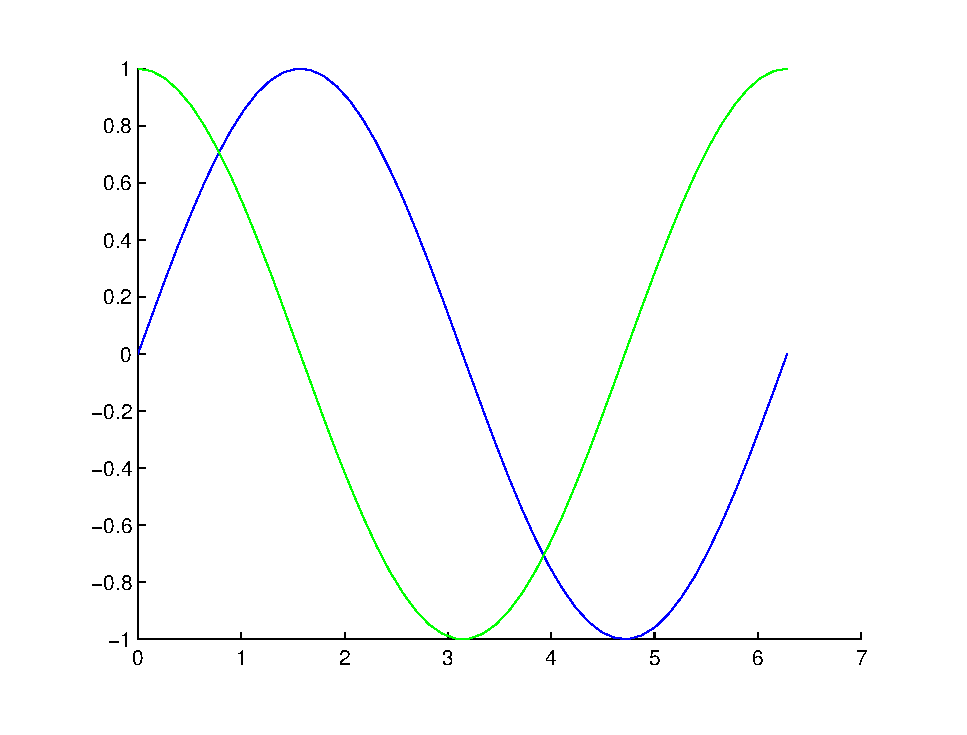
\includegraphics[scale=0.5]{./FiguresMAT/plot2}
\end{matlab}
\caption{$f(x) = \sin{x}$ and $f'(x) = \cos{x}$. Note the color choice makes for better presentation.}
\end{center}
\end{figure}

\begin{problem}  Using the MATLAB documentation and the aforementioned commands, do the following:
\begin{itemize}
\item Generate 25 data points from a distribution of your choosing.  Plot the data points and the least squares regression line on the same plot.  Use different colors and symbols for the data and the regression line.
\item 
\end{itemize}
\end{problem}

\subsection{Changing the \li{plot} window}

Within in MATLAB we have several options for changing the \li{plot} window.  This includes adding captions and other labels, legends, and altering the axes (among other things).  For example, we plot 3 trajectories of a projectile shot from a cannon at 30 meters per second.

\begin{matlab}
\begin{lstlisting}[style=matlab]
g = 9.8;
v = 30;
t = linspace(0,6,100);

h1 = @(t) v*sin(pi/6).*t - 0.5*g.*t.^2;
h2 = @(t) v*sin(pi/4).*t - 0.5*g.*t.^2;
h3 = @(t) v*sin(pi/3).*t - 0.5*g.*t.^2;

hold on;
plot(v*cos(pi/6)*t,h1(t),'color','green')
plot(v*cos(pi/4)*t,h2(t),'color','blue')
plot(v*cos(pi/3)*t,h3(t),'color', 'red')
axis([0 100 0 40]);
xlabel('Distance');
ylabel('Height');
hold off;
\end{lstlisting}
\end{matlab}

See figure 37.4

\begin{figure}
\begin{center}
\begin{matlab}
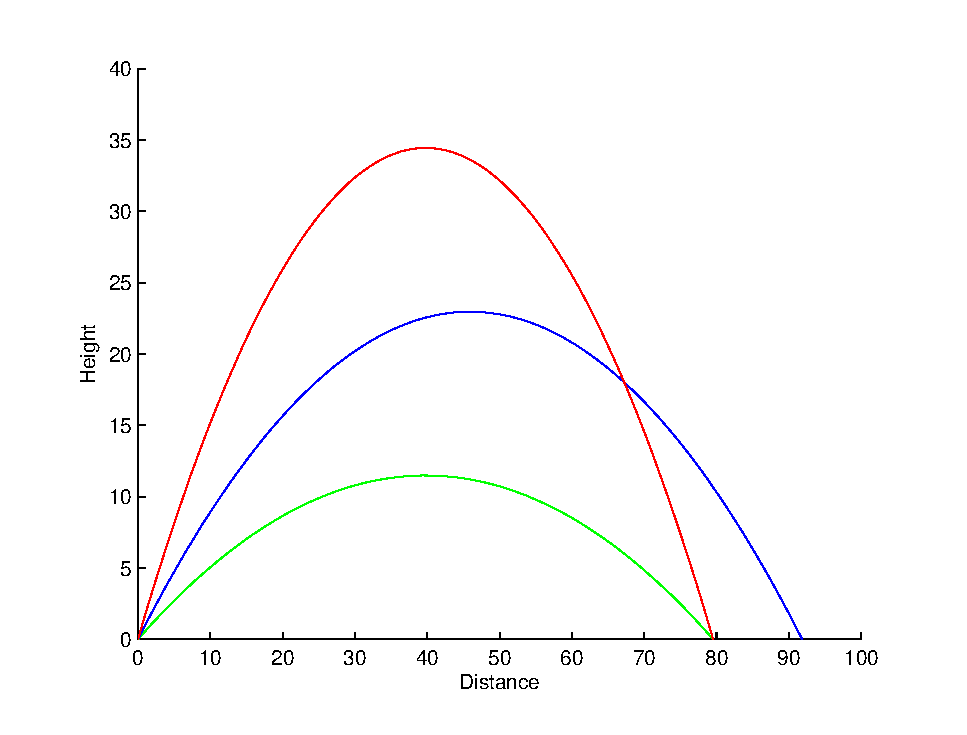
\includegraphics[scale=0.5]{./FiguresMAT/plot4}
\end{matlab}
\caption{Trajectory of a projectile fired at three different angles.}
\end{center}
\end{figure}

\begin{problem} 
\end{problem}

\section{The \li{subplot} command}  Often times we want to include two or more plots in a single figure.  This is done using the \li{subplot} command.  This command will break the plot window into an $m\times n$ matrix of plots.  The subplot windows are numbered starting at $1$ in the top left cell and then ascending from left to right, top to bottom.  For example, instead of using different colors on the previous example, we could do 3 separate plots in a single window.  We could also include a graph of, for example, vertical velocity vs. time, which is informative but unable to be included in the same plot since it requires different units.  Let's see how this is done.

\begin{matlab}
\begin{lstlisting}[style=matlab]
g = 9.8;
v = 30;
t = linspace(0,6,100);

h1 = @(t) v*sin(pi/6).*t - 0.5*g.*t.^2;
h2 = @(t) v*sin(pi/4).*t - 0.5*g.*t.^2;
h3 = @(t) v*sin(pi/3).*t - 0.5*g.*t.^2;

subplot(221); plot(v*cos(pi/6)*t,h1(t),'color','green'); 
axis([0 100 0 40]);
xlabel('Distance');
ylabel('Height');
title('30 degrees')

subplot(222); plot(t, v*sin(pi/6) - g*t,'color','green');
xlabel('Time');
ylabel('Vertical Velocity');

subplot(223); plot(v*cos(pi/4)*t,h2(t),'color','blue');
axis([0 100 0 40]);
xlabel('Distance');
ylabel('Height');
title('45 degrees')

subplot(224); plot(t, v*sin(pi/4) - g*t, 'color','blue');
xlabel('Time');
ylabel('Vertical Velocity');

\end{lstlisting}
\end{matlab}

See figure 37.5.

\begin{figure}
\begin{center}
\begin{matlab}
\includegraphics[scale=0.5]{./FiguresMAT/plot5}
\end{matlab}
\caption{Trajectory of a projectile fired at two different angles and the projectiles corresponding vertical velocity at time $t$.}
\end{center}
\end{figure}

\section{Time graphics?}



%Not yet written
\end{matlab}

\begin{python}
\lab{Algorithms}{Scientific Visualization}{Scientific Visualization}

\objective{Go over techniques for making publication ready figures and making other pretty things.}

Python and SciPy have no builtin plotting capbilities.  These capabilites are provided by Matplotlib.  In this lab we will be focusing on producing publication quality figures in Matplotlib using Python and SciPy.  Thus far we have produced many different plots for several applications.  Here we will focus on different ways of presenting those plots so that they are more informative and aesthetically pleasing.

\section{The \li{pyplot.plot} Command}  
Several of the past labs have required the use of the \li{pyplot.plot} command.  While what we have done so far as been fairly straightforward as far as plotting is concerned, a quick glance at the Matplotlib documentation for \li{pyplot.plot} reveals a plethora of options that can be set to adjust the final plot.

How we use the \li{pyplot.plot} command will vary with our application.  Plotting data requires a very different presentation approach than graphing straight lines.  In the sequel we examine several different options.

\begin{table}[h!]
\begin{center}
	\begin{tabular}{|c|c|}
	
	\hline
	
	Usage & Property Options\\
	
	\hline
	
	\li{color} & \li{yellow, green, blue} etc., or user defined colors \\& given by $[r g b]$, a three element red, green, \\& blue vector.  See documentation for full list. \\
	
	\hline
	
	\li{linestyle} & \li{-, --, :, -., 'None'} \\
	
	\hline
	
	\li{linewidth} & Width in points.  $1$ point is $\frac{1}{72}$ inch.  Default is $1.0$ points. \\
	
	\hline
	
	\li{marker} & \li{+, *, x, .} etc. See documentation for full list. \\
	
	\hline
	\end{tabular}
\end{center}
\caption{Common Plot commands in MATLAB}
\end{table}

For example, if we wanted to plot $f(x) = x^2$, we don't need to extend our typical plotting knowledge much, except maybe we like green better than blue:

\begin{lstlisting}[style=python]
: import matplotlib.pyplot as plt
: import scipy as sp
: x = sp.linspace(-1,5,50)
: f = lambda x: x**2
: plt.plot(x, map(f, x), color='green')
: plt.show()
\end{lstlisting}

See figure 37.1.

\begin{figure}
\begin{center}
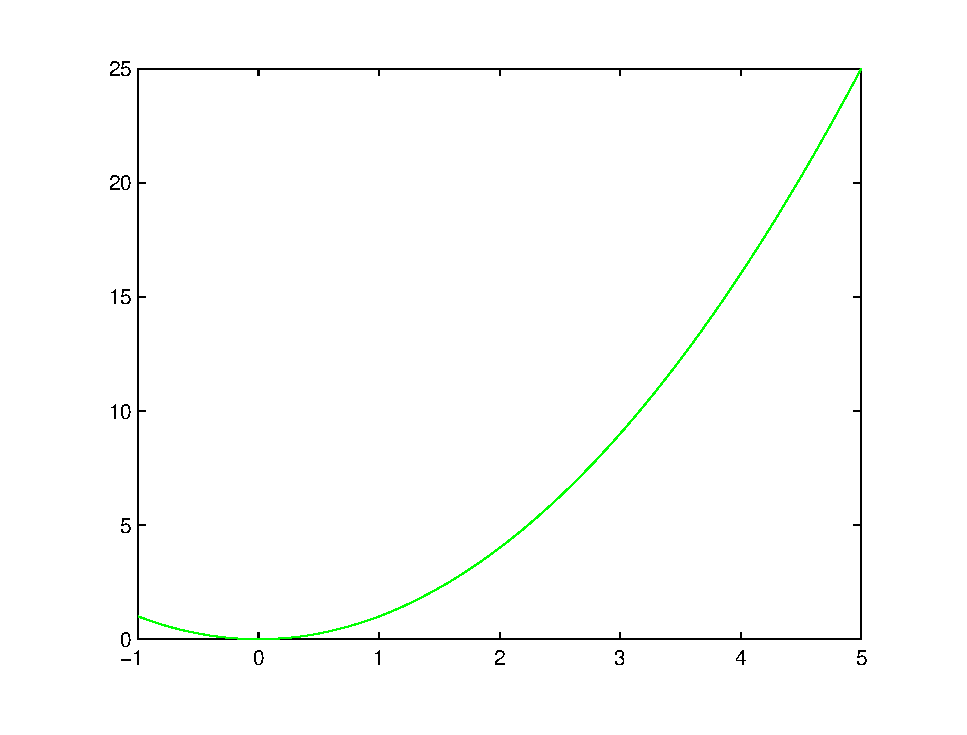
\includegraphics[scale=0.5]{./FiguresMAT/plot1}
\caption{Graph of $f(x) = x^2$}
\end{center}
\end{figure}


However, if we wanted to plot the data drawn from a certain distribution, we would want to use the plot command in a very different way.  For example:

%Explain the code?
\begin{lstlisting}[style=python]
>> X = random('Normal',0,1,[100,1]);
>> plot(X,'marker','*','LineStyle','none');
\end{lstlisting}

See figure 37.2.

\begin{figure}
\begin{center}
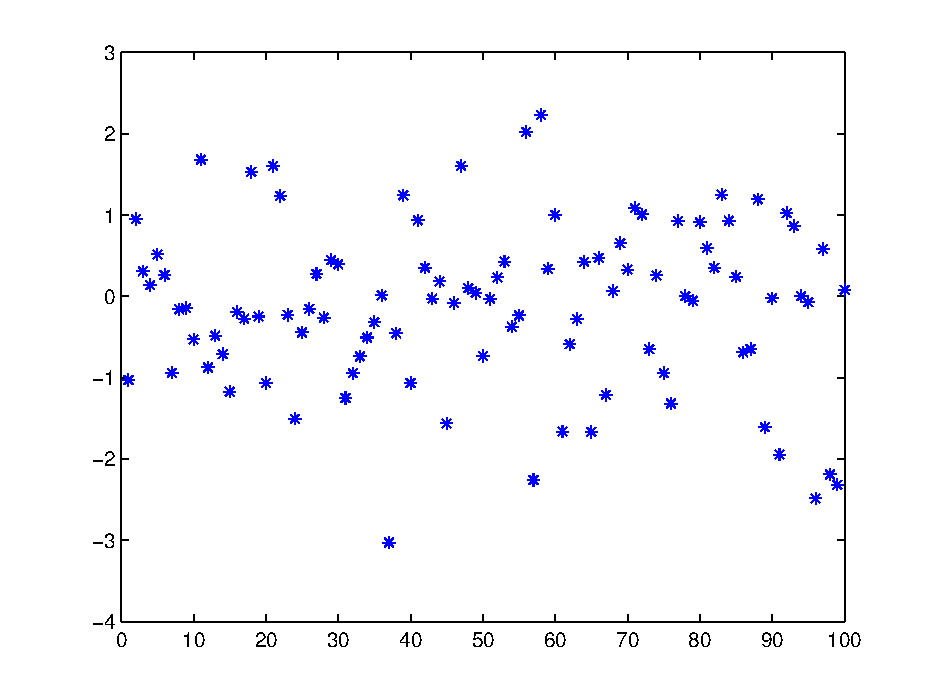
\includegraphics[scale=0.5]{./FiguresMAT/plot3}
\caption{100 data points pulled from a normal distribution}
\end{center}
\end{figure}

The \li{hold} command will also be useful for when plotting more than one graph on a single plot.  For example, if we wanted to graph $f(x) = \sin{x}$ and it's derivative $f'(x) = \cos{x}$, we would do the following:

\begin{lstlisting}[style=python]
: f = lambda x: sp.sin(x)
: df = lambda x: sp.cos(x)
: x = sp.linspace(0,2*sp.pi, 50)
: plt.hold(True)
: plot(x, map(f, x), color='blue')
: plot(x, map(df, x), color='green')
: plt.hold(False)
: plt.show()
\end{lstlisting}

See figure 37.3.

\begin{figure}
\begin{center}
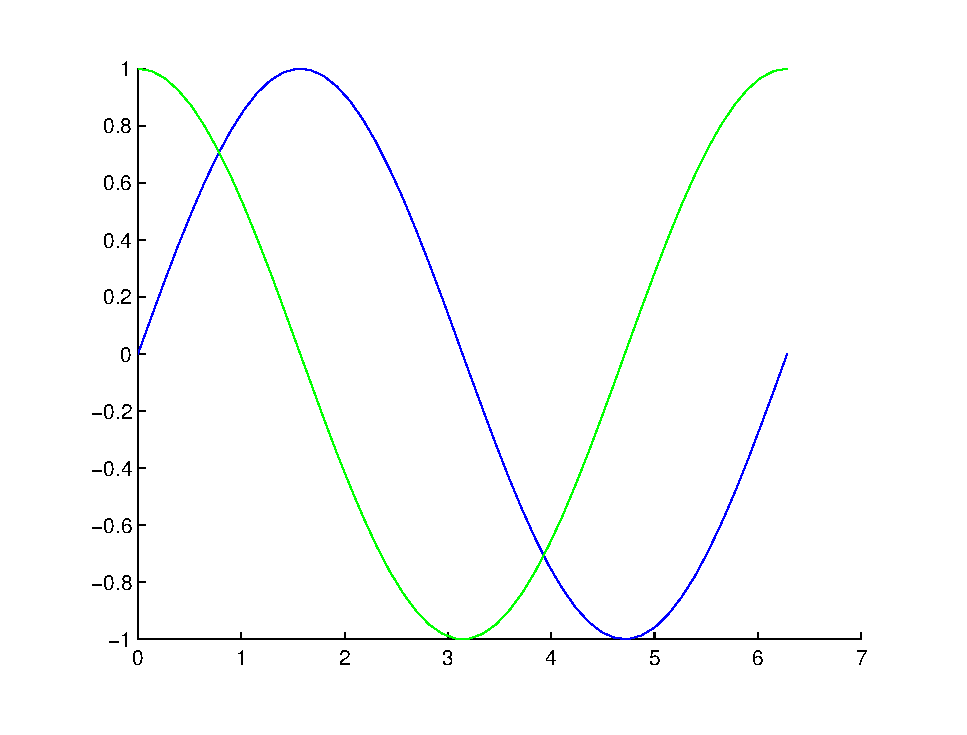
\includegraphics[scale=0.5]{./FiguresMAT/plot2}
\caption{$f(x) = \sin{x}$ and $f'(x) = \cos{x}$. Note the color choice makes for better presentation.}
\end{center}
\end{figure}

\begin{problem}  Using the MATLAB documentation and the aforementioned commands, do the following:
\begin{itemize}
\item Generate 25 data points from a distribution of your choosing.  Plot the data points and the least squares regression line on the same plot.  Use different colors and symbols for the data and the regression line.
\item 
\end{itemize}
\end{problem}

\subsection{Changing the Plot window}

Within in MATLAB we have several options for changing the \li{plot} window.  This includes adding captions and other labels, legends, and altering the axes (among other things).  For example, we plot 3 trajectories of a projectile shot from a cannon at 30 meters per second.

\begin{lstlisting}[style=python]
: g = 9.8
: v = 30.0
: t = linspace(0,6,100)
:
: h1 = lambda t: v*sp.math.sin(sp.pi/6)*t-0.5*g*t**2
: h2 = lambda t: v*sp.math.sin(sp.pi/4)*t-0.5*g*t**2
: h3 = lambda t: v*sp.math.sin(sp.pi/3)*t-0.5*g*t**2
:
: plt.hold(True)
: plt.plot(v*sp.math.cos(sp.pi/6)*t, map(h1, t), color='green')
: plt.plot(v*sp.math.cos(sp.pi/4)*t, map(h2, t), color='blue')
: plt.plot(v*sp.math.cos(sp.pi/3)*t, map(h3, t), color='red')
: plt.axis([0, 100, 0, 40])
: plt.xlabel('Distance')
: plt.ylabel('Height')
: plt.hold(False)
: plt.show()
\end{lstlisting}

See figure 37.4

\begin{figure}
\begin{center}
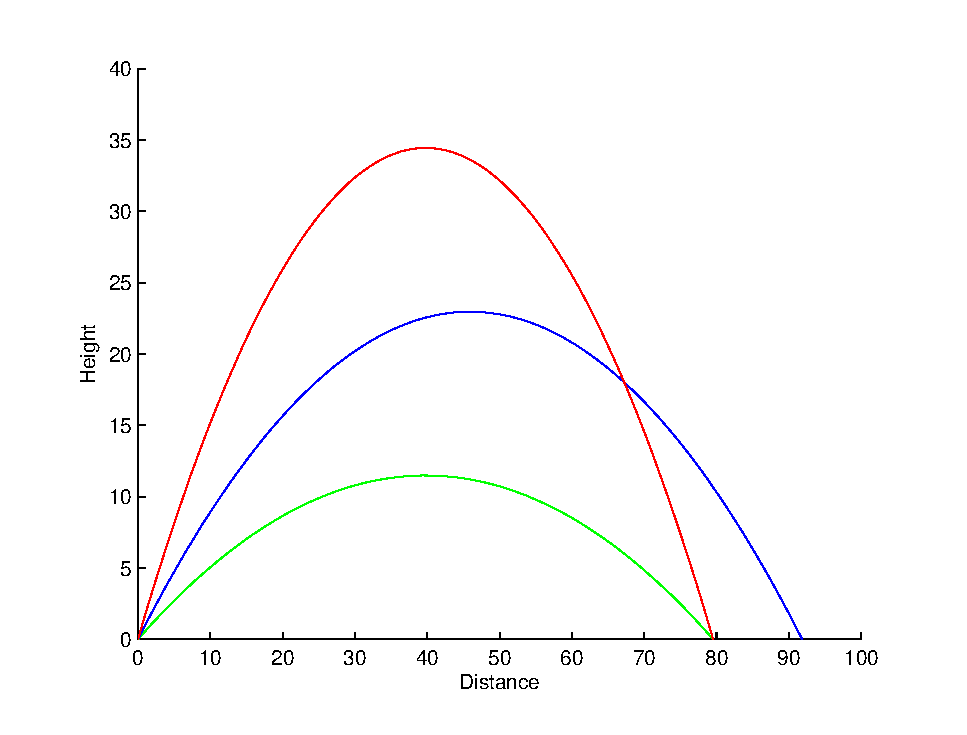
\includegraphics[scale=0.5]{./FiguresMAT/plot4}
\caption{Trajectory of a projectile fired at three different angles.}
\end{center}
\end{figure}

\begin{problem} 
\end{problem}

\section{The \li{subplot} command}  
Often times we want to include two or more plots in a single figure.  This is done using the \li{subplot} command.  This command will break the plot window into an $m\times n$ matrix of plots.  The subplot windows are numbered starting at $1$ in the top left cell and then ascending from left to right, top to bottom.  For example, instead of using different colors on the previous example, we could do 3 separate plots in a single window.  We could also include a graph of, for example, vertical velocity vs. time, which is informative but unable to be included in the same plot since it requires different units.  Let's see how this is done.

\begin{lstlisting}[style=python]
: g = 9.8
: v = 30.0
: t = linspace(0,6,100)
:
: h1 = lambda t: v*sp.math.sin(sp.pi/6)*t-0.5*g*t**2
: h2 = lambda t: v*sp.math.sin(sp.pi/4)*t-0.5*g*t**2
: h3 = lambda t: v*sp.math.sin(sp.pi/3)*t-0.5*g*t**2
:
: plt.subplot(221)
: plt.plot(v*cos(pi/6)*t,h1(t),'color','green')
: plt.axis([0 100 0 40])
: plt.xlabel('Distance')
: plt.ylabel('Height')
: plt.title('30 degrees')
:
: plt.subplot(222)
: plt.plot(t, v*sin(pi/6) - g*t,'color','green')
: plt.xlabel('Time')
: plt.ylabel('Vertical Velocity')
:
: plt.subplot(223)
: plt.plot(v*cos(pi/4)*t,h2(t),'color','blue')
: plt.axis([0 100 0 40])
: plt.xlabel('Distance')
: plt.ylabel('Height')
: plt.title('45 degrees')
:
: plt.subplot(224)
: plt.plot(t, v*sin(pi/4) - g*t, 'color','blue')
: plt.xlabel('Time')
: plt.ylabel('Vertical Velocity')
\end{lstlisting}

See figure 37.5.

\begin{figure}
\begin{center}
%\includegraphics[scale=0.5]{./Figures/plot5}
\caption{Trajectory of a projectile fired at two different angles and the projectiles corresponding vertical velocity at time $t$.}
\end{center}
\end{figure}

\section{Time graphics?}



%Needs to be translated after its written
\end{python}

%---------------------------------------------------------------
%A few labs related to complex mappings and the perspective transform. These labs are combined.

%These labs need translation and merging

\lab{Algorithms}{Conformal Maps}{Conformal Maps}

\objective{To become familiar with some of the basic properties of conformal maps and some of their basic applications.}

The analysis of complex valued functions has been called ``one of the most beautiful and useful fields of mathematics.''  Conformal maps are special functions in complex analysis that have proven to be very useful in several applications, especially those that model physical phenomena.

We begin by examining some maps on the complex plane.  Let
\[
f(z) = \frac{3z - 4}{z - 2}
\]
and
\[
g(z) = z^2 - 2
\]
What happens if we map the box $[0,1]\times[0,i]$ under these mappings?  
\newpage
Looking at $g(z)$, we see the box turn into a sort of curved triangle.  On the other hand, if we look at $f(z)$, it seems like there is even more distortion than in the case of $g(z)$.
\begin{figure}
\begin{center}
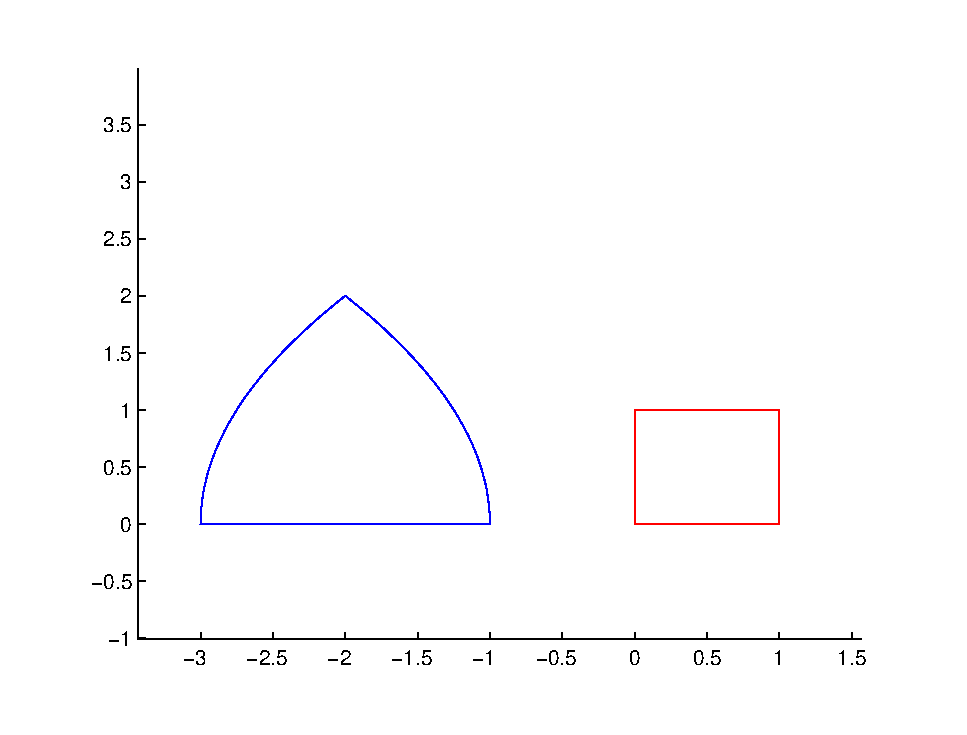
\includegraphics[scale=0.5]{./Applications_Combined/ConfMaps/map1}
\caption{The box $[0,1]\times[0,i]$ under g(z).  The vertical axis is the imaginary line and the horizontal axis is the real line.}
\end{center}
\end{figure}

\begin{figure}
\begin{center}
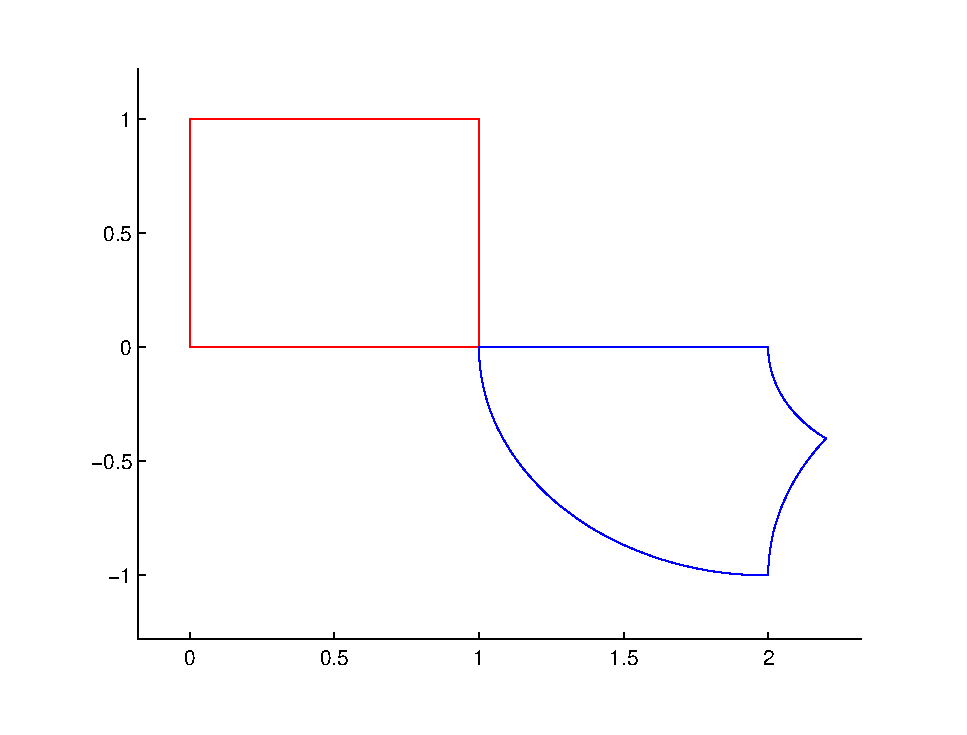
\includegraphics[scale=0.5]{./Applications_Combined/ConfMaps/map2}
\caption{bla bla bla}
\end{center}
\end{figure}

There is a fundamental difference between these two mappings.  Though in both cases the shape is significantly distorted, in the case of $f(z)$ the angles where two sides meet are preserved, whereas $g(z)$ distorts not only the shape of the lines but also the angles where they meet.  Maps that preserve angles, as in the case of $f(z)$, are called conformal.

\begin{figure}
\begin{center}
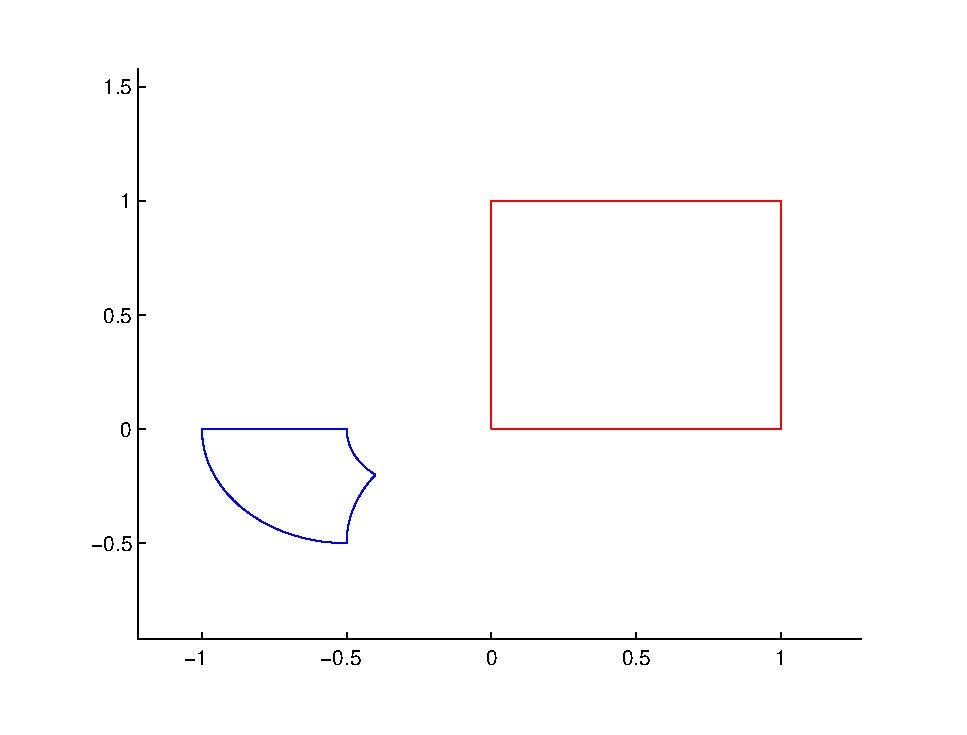
\includegraphics[scale=0.33]{./Applications_Combined/ConfMaps/map3}
\includegraphics[scale=0.33]{./Applications_Combined/ConfMaps/map4}
%\includegraphics[scale=0.33]{./Applications_Labs/ConfMaps/map5}
\caption{Some more conformal maps}
\end{center}
\end{figure}

\begin{problem}
Write a \ProgrammingLanguage script that transform a shape on the complex plane using the the conformal maps that we have used in the examples.  What do you expect will happen to the unit circle on the complex plane under these transformations?  Do your predictions match the results?  Try this for several shapes.
\end{problem}

The theory of conformal mappings is highly developed and well studied.  Here we only scratch the surface and comment on an important theorem for applications that will be useful in later volumes.

\section*{The Schwarz-Christoffel Transformation}
This transformation is very useful in applications of complex analysis.  Once again, the theory behind this is very rich, and we only state a theorem and look at some simple implications here.

\begin{theorem}  Let $P$ be a polygon on the complex plane having consecutive corners at $z_1, z_2, ..., z_n$ with corresponding right turn angles $\theta_1, \theta_2,...\theta_n$.  Then there exists a function that is a one to one conformal map from the upper half plane onto the interior of $P$ of the form:
\[
f(z) = A\int_0^z (\zeta - x_1)^{\frac{\theta_1}{\pi}}..(\zeta - x_{n-1})^{\frac{\theta_{n-1}}{\pi}}d\zeta + B
\]
Where $\theta_i$ represents the angle made by adjacent sides of the polygon and $x_i \in \mathbb{R}$.
\end{theorem}

We omit the proof here.  Consider the power of this theorem - we are able to map the upper half of the complex plane onto a polygon of our choosing.  This is very powerful for finding the numerical solutions to differential equations that model physical systems.  It turns out that a conformal mapping retains sufficient structure of a domain so that a solution in a transformed domain will be the same as the solution in the original domain.  This fact along with the theorem allows us to take problems which may be very difficult to solve in one domain and transform the domain to a polygonal domain of our choosing where a solution is much easier to find.  We give an example of such a transformation using built in \ProgrammingLanguage functions:

\begin{example}
We will give an example showing how to find a Schwarz-Christoffel transform.  Suppose we wish to transform the upper half plane onto the triangle with corners at $0, i,$ and $1$.  We choose $x_1 = -1$ and $x_2 = 1$.  Starting from the upper corner, we have $\theta_1 = \theta_2 = \frac{-3\pi}{4}$ and $\theta_3 = \frac{-\pi}{2}$.  Using theorem 36.1, we have an expression for our mapping:
\begin{align*}
f(z) &= A\int_0^z(\zeta + 1)^{\frac{-3}{4}}(\zeta - 1)^{\frac{-3}{4}}d\zeta + B \\
	 &= A\int_0^z(\zeta^2 - 1)^{\frac{-3}{4}}d\zeta + B
\end{align*}

\end{example}

\begin{problem}
Find the conformal map that transforms the upper half plane to the strip $|Re(z) < 1|, Im(z) > 0$.  Display the result in a meaningful way.
\end{problem}
% (FWG) --There wasn't any code to translate?

\lab{Algorithms}{Perspective Transform}{Perspective Transform}

\objective{Understand the Perspective Transform in three dimensions.}

{\bf Outline:}

\begin{itemize}
\item Explain the physics of a pinhole camera. Explain that mathematically the human eye is similar.
\item We can model any type of camera in a similar manner(we usually just move the focal plane to the other side of the aperture so that the image on the focal plane is right-side up).
\item This allows us to render what a viewer will really see. Used widely in computer graphics, graphic design etc. (in art/graphic design it's related to train tracks meeting at infinity).
\item The math involved: Homogenous coordinates (let you differentiate between vectors and points).
\item Generating rotation matrices. This uses some group theory and matrix exponentials.
\item Explain full-blown Perspective Transform.
\end{itemize}

\begin{problem}
Write a function that accepts a camera location, a viewing direction, a distance to the focal plane and a matrix of points$(n\times 3)$. Have the function return the points as seen on the focal plane (a $(n\times 2)$ matrix).
\end{problem}

\begin{problem}
Discretize some shape (either the MATLAB L or peaks or the Utah Teapot) and render it using the perspective transform. Maybe create an animated gif flyby?
\end{problem}

%Needs to be written
\lab{Applications}{Riemann Sphere and Mobius Transformations}{Riemann Sphere and Mobius Transformations}

\objective{Understand the Riemann Sphere in graphics applications.}

We have now examined several applications of complex numbers and functions.  In this lab we extend several of these ideas and develop some intuition about the Riemann sphere using visualization techniques in \ProgrammingLanguage.

Recall that the complex numbers are an extension of the real numbers that include the imaginary numbers.  We extend them even further in this section and examine the extended complex numbers.  Similar to the extended real numbers, the extended complex numbers are our regular set of complex numbers with the addition of positive and negative infinity.  This allows us to examine, for example, certain quotients that are undefined on the standard complex numbers.

The Riemann sphere construction allows a compact and intuitive construction of the extended complex numbers.  Consider the standard complex plane, only now in 3-space instead of a 2 dimensional plane.  Let the plane pass threw the z-axis at $0$.

{\bf PICTURE HERE}

Now consider a the unit sphere combined with the complex numbers in 3-space:

{\bf PICTURE HERE}

We say that the point at the top of the sphere is positive infinity, while the point at the bottom of the sphere is negative infinity.  We are able to construct any point on the complex plane as the point where a line going from either positive or negative infinity and intersecting the sphere at one point.  Such a line can be constructed to intersect the complex plane at any point of our choosing.  Here are some examples:

{\bf PICTURE AND GOOD CAPTION HERE}.

How do we construct such a line?  Using our understanding of lines in 3 space the construction is rather straightforward.

\begin{problem}  Find the point on the Riemann sphere that along with the point at infinity, creates the line that intersects the complex plane at $1 + 5i$, $10 + 15i$, and $1000 + 1500i$.  Why do we say that the top and bottom of the sphere are infinities?  Draw these lines and the Riemann sphere in \ProgrammingLanguage.  Write a function that, given a point on the complex plane, finds the corresponding point on the Riemann sphere and visualizes it.
\end{problem}

\section*{Mobius Transformations}

Recall from chapter {\bf ???} that a conformal mapping is a complex function that preserves angles between lines.  We now examine a special kind of conformal mapping called a Mobius transformation.  We first give the definition of the Mobius transform, and then examine what sorts of transformations we can do with them.

\begin{definition}  A Mobius transformation is a any complex function of the form
\[
f(z) = \frac{az + b}{cz + d}
\]
With the restriction that $ad \neq bc$
\end{definition}

The Mobius transformation is versatile enough to include translations, rotations, magnifications, or any combination of the same, of shapes in the complex plane.  For example, if we wish to translate the unit disk on the complex plane and then magnify it two times, we would use the following transformation:
\[
PUT IT HERE
\]

{\bf PICTURE GOES HERE}

\begin{problem} Write a \ProgrammingLanguage function that accepts arguments $a,b,c,$ and $d$.  Perform the corresponding Mobius transformation on a grid inside the box $[-1,1]\times[-i,i]$, and then visualize the box before and after the transformation on the same plot, but using different colors.
\end{problem}

What do these special transformations have to do with the Riemann sphere?  Recall from the conformal maps chapter that we can construct any point on the complex plane by drawing a line from infinity through a point on the Riemann sphere.  Consider the points on the sphere that can be used to construct the grid in the previous problem.

{\bf PICTURE GOES HERE}

It turns out that we can express any Mobius transformation as a translation or rotation of the Riemann sphere.  For example:

{\bf SEVERAL PICTURES WITH GOOD CAPTIONS GO HERE}

EXAMPLE OF HOW TO FIND THE TRANSFORMATION OF THE SPHERE HERE

\begin{problem}  Write a \ProgrammingLanguage program that extends the previous problem to 3-dimensions.  Visualize the Mobius translation as a rotation/translation of the Riemann sphere.
\end{problem}



%Partially written

%---------------------------------------------------------------
%These labs cover plotting and visualization. They will be separated by language

\begin{matlab}
\lab{Algorithms}{Graphics Handles}{Graphics Handles}

\objective{Understand the the use of graphics handles in applications.}

{\bf Outline}

\begin{itemize}
\item Explain that the plot tool is a little unwieldy. We can use plot handles to adjust plots directly.
\item Give examples of being able to modify specific data sets on a plot, and change plot properties with ease. Include: YData, text, mesh vs. surf, scale, axes etc.
\item Essentially the point is to be able to modify plots directly.
\item Introduce MATLAB GUI's. This will require a little bit of work, but could be pretty cool. Uses the idea of handles to manipulate user input.
\end{itemize}

\begin{problem}
Write a script that changes every time the user hits enter. Maybe the logistic or horseshoe map (that could be a fun intro to chaos). Or, less interestingly, have sine with different frequencies.
\end{problem}

\begin{problem}
Make a gui that changes the frequency of sine based upon a slider. Now add a set of checkboxes that allows us to show sine and/or cosine.
\end{problem}

\begin{problem}
Implement a gui on the Julia Sets problems, allowing modification of parameters.
\end{problem}%Needs to be written
\lab{Applications}{Time Delayed Graphics}{Time Delayed Graphics}

\objective{Heat equation and shockwaves and such.}

%Needs to be written

\lab{Algorithms}{Motion in 3D}{Motion in 3 Dimensions}

\objective{How to use MATLAB to make neat things move in 3d.}

{\bf Outline:}

\begin{itemize}
\item One use of graphics handles is to allow simulated motion in 3D. This can be particularly useful in graphics applications.
\item Walkthrough building an object and animating it. I think a good object might be attached pendulums (you get cool, non-trivial, chaotic sorts of motion). Following Dr. Beard's method for the helicopter is probably a good idea.
\item I think that this walkthrough will probably take most of the space. The idea really is to give them a good idea of how it could be done...
\end{itemize}

\begin{problem}
Model the solar system and make it move. Maybe  just the inner planets is a good idea. Use elliptical orbits, with accurate orbital speeds (maybe give a simplified table).
\end{problem}%Needs to be written
\end{matlab}

\begin{python} 
\lab{Algorithms}{Graphics Handles}{Graphics Handles}

\objective{Understand the the use of graphics handles in applications.}

{\bf Outline}

\begin{itemize}
\item Explain that the plot tool is a little unwieldy. We can use plot handles to adjust plots directly.
\item Give examples of being able to modify specific data sets on a plot, and change plot properties with ease. Include: YData, text, mesh vs. surf, scale, axes etc.
\item Essentially the point is to be able to modify plots directly.
\item Introduce MATLAB GUI's. This will require a little bit of work, but could be pretty cool. Uses the idea of handles to manipulate user input.
\end{itemize}

\begin{problem}
Write a script that changes every time the user hits enter. Maybe the logistic or horseshoe map (that could be a fun intro to chaos). Or, less interestingly, have sine with different frequencies.
\end{problem}

\begin{problem}
Make a gui that changes the frequency of sine based upon a slider. Now add a set of checkboxes that allows us to show sine and/or cosine.
\end{problem}

\begin{problem}
Implement a gui on the Julia Sets problems, allowing modification of parameters.
\end{problem}%Stub. Will need to be updated once written.
\lab{Applications}{Time Delayed Graphics}{Time Delayed Graphics}

\objective{Heat equation and shockwaves and such.}

%Stub. Will need to be updated once written.

\lab{Algorithms}{Motion in 3D}{Motion in 3 Dimensions}

\objective{How to use MATLAB to make neat things move in 3d.}

{\bf Outline:}

\begin{itemize}
\item One use of graphics handles is to allow simulated motion in 3D. This can be particularly useful in graphics applications.
\item Walkthrough building an object and animating it. I think a good object might be attached pendulums (you get cool, non-trivial, chaotic sorts of motion). Following Dr. Beard's method for the helicopter is probably a good idea.
\item I think that this walkthrough will probably take most of the space. The idea really is to give them a good idea of how it could be done...
\end{itemize}

\begin{problem}
Model the solar system and make it move. Maybe  just the inner planets is a good idea. Use elliptical orbits, with accurate orbital speeds (maybe give a simplified table).
\end{problem}%Stub. Will need to be updated once written.
\end{python}

%----------------------------------------------------------------
%These labs cover a wide variety of applications, and finish off the book. They will be combined

\lab{Applications}{Ray Tracing}{Ray Tracing}

\objective{Understand and implement some ray tracing stuff}

{\bf Outline}

\begin{itemize}
\item Explain the problem of simulating light being cast from a source: most of it doesn't make it to the camera.
\item Explain the approach of raytracing: go backwards from the camera.
\item Different types of rays: reflection refraction and shadow.
\item Work an example of shadow maybe (sphere shaded partially by a cube)?
\item Explain computational burden (lots of rays). Tradeoff between realism and speed. Used more in applications that can take time (such as movies).
\item Explain refraction well (angles incident to surface etc.).
\end{itemize}

\begin{problem}
Model a movie screen with a glass shape (ellipse? Sphere?) between the viewer and the screen. What does the movie look like? This will combine refraction and raytracting.
\end{problem}

%To be written

\lab{Algorithms}{Jordan Forms and Schur Decompisition}{Jordan Forms and Schur Decomposition}

\objective{Learn about Jordan forms, what we would like to use them for, and why we use Schur decomposition instead.}

%To be written
\lab{Applications}{Lagrange-Sylvester Interpolation}{Lagrange-Sylvester Interpolation}

\objective{Lagrange-Sylvester Interpolation.}

%To be written

\lab{Algorithms}{Krylov Subspaces}{Krylov Subspaces and Minimal Polynomials}

\objective{Krylov Subspaces and Minimal Polynomials}

%To be written
\lab{Applications}{Perron Frobenius Theorem}{Markov Chains and the Perron Frobenius Theorem}

\objective{Markov Chains and the Perron Frobenius Theorem}

%To be written

\lab{Algorithms}{Moore-Penrose Pseudo-Inverse}{Moore-Penrose}

\objective{This section explains several methods for numerically computing the Moore-Penrose Pseudo-Inverse. It also compares performance of the different methods.}
 
The generalized inverse of a matrix $A$ is a matrix (which we will denote $A^\dagger$ for now) that satisfies the following:
\begin{equation} \label{cond:one}
AA^\dagger A = A 
\end{equation}

\begin{equation} \label{cond:two}
A^\dagger A A^\dagger = A^\dagger 
\end{equation}

For any matrix $A$ there exists a generalized inverse. Note that in the case that $A$ is invertible, $A^{-1}$ satisfies the conditions \ref{cond:one} and \ref{cond:two}. However, it is not generally unique. For this reason, we usually add additional conditions that make the generalized inverse unique.

For example, we can specify the following two additional conditions:

\begin{equation} \label{cond:three}
(AA^\dagger)^* = AA^\dagger
\end{equation}

\begin{equation} \label{cond:four}
(A^\dagger A)^* = A^\dagger A
\end{equation}

These four conditions guarantee both the existence and uniqueness of the matrix $A^\dagger$ for any matrix $A$. The matrix $A^\dagger$ is known as the Moore-Penrose inverse. In some settings it is simply called the pseudo-inverse.\footnote{For the rest of this section we will use the notation $A^\dagger$ to represent the moore-penrose inverse, although in some books that notation is used a generalized inverse}

{\bf We could add some exposition here about examples of the MP inverse for specific matrices, but I don't know if Jeff is doing that in the book or not...}

\subsection{Calculating the Moore-Penrose Inverse}

There are several different methods for calculating the Moore-Penrose Inverse. We will consider the most general method first, and then compare its performance to a few specialized methods.

Recall that the SVD of a matrix $A$ is of the form

\[
A = U \Sigma V^*
\]

Where $U$ and $V$ are unitary (i.e. $U^*U = I$) and $\Sigma$ is diagonal. Consider the matrix

\[
B = V \Sigma^\dagger U^*
\]

Where $\Sigma^\dagger$ is the pseudo-inverse of $\Sigma$. Since $\Sigma$ is diagonal, the pseudo-inverse is simply found by replacing each non-zero entry with its multiplicative inverse and transposing the matrix. We write, for ease of notation $\Sigma^\dagger \Sigma = I_A$ Now we have the following:

\[
ABA = U \Sigma V^* = A
\]

\[
BAB = V \Sigma^\dagger U^* = B
\]

\[
(AB)^* = U \Sigma^{\dagger *} V^* V \Sigma^* U^* = U (\Sigma \Sigma^\dagger)^* U^* = U \Sigma \Sigma^\dagger U^* = U \Sigma V^* V \Sigma^\dagger U^* = AB
\]

\[
(BA)^* =  V \Sigma^* U^* U \Sigma^{\dagger *} V^* = V (\Sigma^\dagger \Sigma)^* V^* = V  \Sigma^\dagger \Sigma V^* =  V \Sigma^\dagger U^* U \Sigma V^* = BA
\]

Thus $B$ satisfies all of the properties of the pseudo-inverse, and since the pseudo-inverse is unique it is the only such matrix.

Therefore, we can easily calculate the pseudo-inverse of a matrix using the SVD. Write the following code in \ProgrammingLanguage :

\begin{matlab}
\begin{lstlisting}[style=matlab]
[U,S,V] = svd(A,'econ');
\end{lstlisting}
\end{matlab}
\begin{python}
\begin{lstlisting}[style=python]
U,s,Vh = la.svd(A,full_matrices=False)
S = sp.diag(s)
\end{lstlisting}
\end{python}

\begin{matlab}%I don't know if the following is true of the Python version yet
As you recall, in chapter three we talked about how the \li{econ} option for the \li{svd} function makes the SVD representation as compact as possible, by eliminating the sections of $\Sigma$ that are zeros, and the corresponding parts of $U$ and $V$. \end{matlab}We can then calculate the pseudo-inverse by using the following line of code:

\begin{matlab}
\begin{lstlisting}[style=matlab]
Apinv = V*diag(1./diag(S))*U';
\end{lstlisting}
\end{matlab}
\begin{python}
\begin{lstlisting}[style=python]
Apinv = sp.dot(sp.dot(Vh.T,sp.diag(1./s)),U.T)
\end{lstlisting}
\end{python}

This line uses the matrices that \li{svd} created to calculate the pseudo-inverse, using the formula we established above. Note that we used \li{diag} twice to invert just the singular values (and not the zeros). \begin{matlab}Also note that since we used the \li{econ} option the matrix $S$ is square and hermitian, and therefore we don't have to transpose it.\end{matlab}%still don't know if this is valid for the full_matrices=0 option
\begin{problem}
\begin{matlab}
\ProgrammingLanguage has a built-in function \li{pinv}that calculates the pseudo-inverse. Write a script that compares the performance of \li{pinv} and the implementation that we demonstrated above. Use a matrix generated by  \li{rand}.\end{matlab}
\begin{python}%Python has pinv and pinv2, which appear to differ by algorithms. So which one do we test? - I think pinv2 uses SVD -- here I suggest to test both
\ProgrammingLanguage has the built-in functions \li{la.pinv} and \li{la.pinv2} to calculate the pseudo-inverse. Write a script that compares the performance of \li{la.pinv},\li{la.pinv2}, and the implementation that we demonstrated above. Use a matrix generated by  \li{sp.rand}.\end{python}
 Try the following matrix sizes:
\begin{itemize}
\item $1000 \times 1$
\item $1000 \times 20$
\item $1000 \times 500$
\item $1000 \times 1000$
\end{itemize}
How do the performances compare?
\end{problem}

\begin{problem}
{\bf Continuity of the pseudo-inverse:} This problem demonstrates why the pseudo-inverse is not generally a continous operation. Create a random $5 \times 5$ matrix $A$, and find its SVD using the code:
%should we use 'econ' here? I haven't read whatever section that comes from
\begin{matlab}
\begin{lstlisting}[style=matlab]
[U,S,V] = svd(A)
\end{lstlisting}
\end{matlab}
\begin{python}
\begin{lstlisting}[style=python]
U,s,Vh = la.svd(A,full_matrices=False)
V = Vh.T
S = sp.diag(s)
\end{lstlisting}
\end{python}.
Set the bottom right entry of $S$ to zero, and then set $A = U*S*V'$. Now set $S(5,5)$ to be $.01$. Now calculate \begin{matlab}\li{norm(A - U*S*V')}\end{matlab}\begin{python}\li{la.norm(A - sp.dot(sp.dot(U,S),Vh))}\end{python}. The value should be $.01$. This is because the matrix $2$-norm is simply the value of the largest singular value. Now calculate \begin{matlab}\li{norm(pinv(A) - pinv(U*S*V'))}\end{matlab}\begin{python}\li{la.norm(la.pinv(A) - la.pinv(sp.dot(sp.dot(U,S),Vh)))}\end{python}. You should get $100$. Why is this? Hint: Think of how we calculated the pseudo-inverse. This example, and your explanation, should explain why two matrices, that are arbitrarily close together, can have pseudo-inverses that are arbitrarily far apart. Thus the pseudo-inverse is not a continuous operator.
\end{problem}

\subsection*{Other methods for calculating the Pseudo-Inverse}

The SVD is a powerful tool for calculating the pseudo-inverse. However, for large matrices it can be costly to calculate the SVD. Accordingly, there are several other methods for calculating the pseudo-inverse of a matrix.

One method is an iterative approach established by Ben-Israel and Cohen\footnote{Ben-Israel, Adi; Cohen, Dan (1966). "On Iterative Computation of Generalized Inverses and Associated Projections". SIAM Journal on Numerical Analysis 3: 410–419.}. This method uses the recursive sequence

\[
A_{i+1} = 2A_i - A_i A A_i
\]

With $A_0$ satisfying the equation $A_0 A = (A_0 A)^*$. The convergence of this sequence eventually becomes quadractic, which is a very desirable property. The simplest choice for $A_0$ is $\alpha A^*$, with $0 < \alpha < 2/\sigma_1^2(A)$, where $\sigma_1$ denotes the largest singular value (the condition on $\alpha$ is a technical condition established in the original paper to guarantee fast convergence).

One tricky part of developing this method is finding an appropriate $\alpha$. We don't want to waste much time calculating $\sigma_1$. Luckily there is an easy equivalence that we can leverage:

\[
||A||_2 = \sigma_1(A) = \sqrt{\lambda_{max} (A^* A)}
\]
%Python: no eigs function -- but it appears to be a topic of interest in the community, perhaps a future addition
Thus, we can calculate the largest singular value of $A$ quickly in some cases using \begin{matlab}\li{eigs}\end{matlab}. We stress that this is not always the fastest way. For example, if $A$ is a million by one column vector then calculating the 2-norm of $A$ is much faster than calculating the largest eigenvalue of a million by million matrix. However, with these equivalences we have some tools at our disposal to easily calculate the largest singular value of $A$.

Now, using these tools, we can write a simple function to calculate the pseudo-inverse using this iterative method:

\begin{matlab}
\begin{lstlisting}[style=matlab]
function out = IterativePInv(A)

alpha = 2/(1.1*eigs(A'*A,1));
out = alpha*A';
C = out + 1;
while max(sum(abs(C-out))) > 1e-4
    C = out;
    out = 2*out - out*A*out;
end
\end{lstlisting}
\end{matlab}
\begin{python}
\begin{lstlisting}[style=python]
function out = IterativePInv(A)

alpha = 2/(1.1*eigs(A'*A,1));
out = alpha*A';
C = out + 1;
while max(sum(abs(C-out))) > 1e-4
    C = out;
    out = 2*out - out*A*out;
end
\end{lstlisting}
\end{python}
As you can see, the implementation of this algorithm is fairly straightforward. We used the matrix $1$-norm (the maximum absolute column sum) to detect convergence of our sequence, since it is very fast to compute.

\begin{problem}
The implementation we wrote above is naive in a few ways. Make the following three adaptations to your code:
\begin{itemize}
\item Allow variable tolerance in the detection of convergence of the sequence. Use \begin{matlab}\li{varargin}\end{matlab}\begin{python}\li{*args}\end{python} so that the user only specifies the tolerance if they want to.
\item We used the value $1.1$ rather arbitrarily in our selection of $\alpha$. The original paper proves that the optimal value is $2/(\sigma_1^2 + \sigma_r^2)$, where $\sigma_r$ is the smallest non-zero singular value. Use \begin{matlab}\li{eigs}\end{matlab} again to find the value of $\sigma_r$, and use that value to set $\alpha$.
\item If $A$ isn't close to square then it is not advantageous to use \begin{matlab}\li{eigs}\end{matlab} at all, as we explained above. Adapt the code to only use \li{eigs} as you think it's appropriate. Remember that you can use the matrix $2$-norm and a constant like $1.1$ in cases where \begin{matlab}\li{eigs}\end{matlab} isn't appropriate.
\end{itemize}

Now test your code against the svd method, using the same cases that you did for that method. How does it perform?
\end{problem}

It should be noted that this method, although powerful, sometimes performs worse than the svd method. Specifically, when the matrix is ill-conditioned, it may take a long time for the sequence to enter the region of quadratic convergence, making this method a poor choice.

\subsection*{The QR method}

This final method, while only applicable in certain cases, offers a very fast method for calculating the pseudo-inverse. Suppose that $A$ has full column rank. We could show that the pseudo-inverse is then:
\[
A^\dagger = (A^* A)^{-1} A^*
\]

Direct calculation of the pseudo-inverse using this formula is not very helpful, since matrix inversion is so costly. However, since $A$ is full rank, then $A^*A$ is positive definite, and thus has a cholesky decomposition. Therefore, we can rewrite this equation as:

\[
R^*R A^\dagger = A^*
\]

with $R$ being upper-triangular. This equation can be solved quickly by using forward and backward substitution.

We can speed calculation even further by noting that we don't even have to calculate $A^* A$, which can be costly (again, imagine the million by one vector). We can calculate R using the QR-decomposition of A:

\[
A^* A = R^*Q^*QR = R^* R
\]

These equalities hold since $Q$ is orthogonal. Further, in the QR decomposition $R$ is upper-triangular, and thus we can calculate the cholesky factorization easily using the QR decomposition.

Combining these facts we can write the following code to calculate the pseudo-inverse for a matrix that has full column rank as follows:

\begin{matlab}
\begin{lstlisting}[style=matlab]
R = triu(qr(A));

Ainv = R\(R'\A');
\end{lstlisting}
\end{matlab}
\begin{matlab}
\begin{lstlisting}[style=matlab]
R = la.qr(A)[1];

Ainv = la.lstsq(R,la.lstsq(R.T,A.T)[0])[0];
\end{lstlisting}
\end{matlab}

\begin{matlab}We have to use \li{triu} in the first line because of the conventions used by MATLAB's \li{qr} code.\end{matlab}\begin{python}The first line performs QR decomposition for $R$.\end{python} The second line conducts the backwards and forwards substitutions.

\begin{problem}
%This Problem did not exactly work in Python, my function was slower when A was square when using la.lstsq
Compare the run-time of this code against \ProgrammingLanguage's \begin{matlab}\li{pinv}\end{matlab}\begin{python}\li{la.pinv}\end{python}, for the values used in the other problems. \begin{python}Also, make sure to use a non-square matrix for A, or for square matricies change the \li{la.lstsq}'s to \li{la.solve}'s to maximize performance.\end{python}How does it compare? It should be a lot faster. This demonstrates that by leveraging the correct information (full column rank) we can significantly improve the speed of this operation. Note that we can beat \ProgrammingLanguage's own implementation significantly in this case.

\end{problem}

\begin{problem}
This method can also be adapted to use for matrices that have full row rank. In the case of full column rank the following formula holds:
\[
A^\dagger = A^*(A A^*)^{-1}
\]
Use the same technique to write a function that finds the pseudo-inverse for a matrix of full row rank. Note that you will have to find the QR-decomposition of $A^*$ this time, and that it may be helpful to take the transpose so that you can use the backslash operator.
\end{problem}
%Needs to be translated (FWG) --Python Lacks an eigs command, which makes translation of the middle subsection difficult
\lab{Applications}{Applications of the Pseudo-Inverse}{Pseudo-Inverse Applications}

\objective{This section explains a few applications of the Moore-Penrose inverse, including least squares problems, norm-minimization problems and the condition number.}

The pseudo-inverse is a useful generalization for a variety of applications. The first we will consider is least squares and norm-minimization problems.

Consider the system
\[
Ax = b
\]

$A$ need not be full rank. It may be either over or under-determined. How do we come up with a ``good'' solution to this system? In the case where the system is over-determined, we can use least squares to find the solution that minimizes $\norm{Ax^* - b}_2$. In the case where $A$ is under-determined there may be an infinite number of solutions. Assuming that there is a solution, we will search for the solution that minimizes the norm of the solution, or in other words we will minimize $\norm{x^*}_2$ subject to $Ax-b = 0$.

Amazingly, the pseudo-inverse solves both of these problems. We will offer a brief proof. First, for ease of notation, let $P = A A^\dagger$. Note that $PA = A$ and $P = P^*$. We also denote $z = A^\dagger b$. Using these facts we can show that:
\begin{align*}
A^*(Az-b) &= A^*(A A^\dagger b - b) \\
&= A^*P b - A^* b \\
&= (PA)^* b - A^* b \\
&= 0
\end{align*}

Then we can use the parallelogram law to show that:

\begin{align*}
\norm{Ax-b}_2^2 &= \norm{Ax + Az-Az-b}_2^2 \\
&= \norm{Az-b}_2^2 + (A(x-z))^*(Az-b) + \left((A(x-z))^*(Az-b)\right)^* + \norm{A(x-z)}_2^2 \\
&= \norm{Az-b}_2^2 + ((x-z)^*A^*(Az-b) + \left(((x-z)^*A^*(Az-b)\right)^* + \norm{A(x-z)}_2^2 \\
&= \norm{Az-b}_2^2 + \norm{A(x-z)}_2^2 \\
&\geq \norm{Az-b}_2^2
\end{align*}

Thus, $z$ is the least squares solution.
%I thought I saw this proof somewhere else in the book - is it in here twice?
\begin{problem}
Suppose that $A$ is under-determined and that $Ax = b$ has a solution (i.e. is staisfiable). Use the same steps as we used for the least squares solution to prove that $z = A^\dagger b$ is the minimum norm solution. For the first step, show that expression $z^*(x-z) = 0$. For the second step use the parallelogram rule on $\norm{x -z +z}_2^2$.
\end{problem}

{\bf Here a good problem involving finding the minimum-norm solution of something would be perfect. Do you have any suggestions?}

\subsection*{Condition Number}

Suppose that we have the equation:
\[
Ax= b
\]
Now suppose that we have an approximate solution, namely we have $\tilde{x}$ such that $\norm{A\tilde{x} -b}$ is small. Does this imply that $\norm{x-\tilde{x}}$ is small? This is not always the case. Consider, for example, the system:
\[
\begin{pmatrix}
2 & 1\\
4 & 2.1 \\
\end{pmatrix} x = 
\begin{pmatrix}
3 \\
6.01\\
\end{pmatrix}
\]

This system has the unique solution $x = [1~1]^T$. However, the vector $\tilde{x} = [1.5~0]^T$ has a very small solution error since $\norm{Ax-A\tilde{x}} = .01$, but the difference betwen $[1~1]$ and $[1.5~0]$ is pretty significant. This is an example of what is called an ill-conditioned matrix. The issue in this case, is that the matrix $A$ maps two vectors that are relatively far apart (namely $x$ and $\tilde{x}$) to vectors that are close together.

This issue becomes very important when we're dealing with floating point arithmetic. It isn't hard to imagine that in finite precision arithmetic it might be reasonable to say that $\tilde{x}$ is a solution to the linear equation above, while it is actually very different from the real solution. We note that in this case rounding errors are not to blame! The matrix itself is to blame.

We quantify this behavior with what is called the condition number of a matrix. The condition number, informally, represents the amount that the solution $x$ of the equation $Ax = b$ changes with respect to $b$. Therefore a large condition number implies that a small error in $b$ (from either measurement error, or floating point arithmetic) can yield a large error in the solution $x$. We can calculate the condition number of a matrix using the following equality:
\[
k(A) = \norm{A} \norm{A^\dagger}
\]
Where $k(A)$ represents the condition number of the of matrix $A$. In this case, the choice of norm isn't important. What we are  doing when we change norms is really change the interpretation of the condition number (i.e. what we are using to measure changes in $b$ and $x$)\footnote{The fact that $A^\dagger$ is not continuous can be problematic for the calculation above, but we are not going to treat that problem here}.

For example, in \ProgrammingLanguage we can calculate the condition number of the above matrix using the following code:

\begin{matlab}
\begin{lstlisting}[style=matlab]
>> A = [2 1;4 2.01]
A =
    2.0000    1.0000
    4.0000    2.0100

>> norm(A)*norm(pinv(A))
ans =
   1.2520e+03
\end{lstlisting}
\end{matlab}
\begin{python}
\begin{lstlisting}[style=python]
A = sp.array([[2,1],[4,2.01]])
la.norm(A)*la.norm(la.pinv(A))
\end{lstlisting}
\end{python}

The error that we had in our example was

\[
\frac{\norm{[.5, -1]}}{\norm{[0, .01]}} = 111.8
\]

Which is a whole order of magnitude smaller than the condition number. This implies that the matrix $A$ could give solutions ten times ``worse'' than it did in our example.

Note that \ProgrammingLanguage has a \begin{matlab}\li{cond}\end{matlab} \begin{python}\li{np.linalg.cond}\end{python} function to calculate the condition number of a matrix. You can verify that the output is the same for the example that we just showed. Also, Volume II offers a more in-depth discussion of conditioning.

\begin{problem}
An $n \times n$ Hilbert Matrix is a matrix with the following entries:
\[
H_{ij} = \frac{1}{i + j -1}
\]

This matrix arises in least-squares polynomial approximation. This matrix is also a canonical example of an ill-conditioned matrix. Write a function that accepts $n$ as an argument and calculates the condition number of the n-th Hilbert Matrix. Plot the growth of the condition number with respect to $n$. What conclusion can you draw about using this type of matrix? %What should be the range of n on our plot?
\end{problem}% (FWG)

\lab{Algorithms}{Drazin Inverse}{Drazin Inverse}

\objective{This section explains methods for computing the Drazin Inverse}

In the last section we talked about the Moore-Penrose inverse. Much of the power of the Moore-Penrose Inverse is derived from it's equation solving ability (it gives the least-square solution). However, by doing so, it sacrifices other properties that we expect a matrix to have.

For example the Moore-Penrose Inverse of a Matrix $A$ generally will not satisfy the relations
\begin{equation} \label{eq:DrazinOne}
A A^\dagger = A^\dagger A
\end{equation}

\begin{equation} \label{eq:DrazinTwo}
A^{p+1} A^\dagger = A^p
\end{equation}

\begin{equation} \label{eq:DrazinThree}
\lambda \in \sigma(A) \iff \lambda^{-1} \in \sigma(A^\dagger)
\end{equation}

These properties are all very desirable in certain settings, but the Moore-Penrose Inverse fails to have them generally. Therefore, we develop a different type of inverse that does have these properties: the Drazin Inverse.

First, we define the index of a matrix. The index is the smallest integer $k$ such that $Rank(A^k) = Rank(A^{k+1})$. We then define the drazin inverse, $A^D$, as the matrix that satisfies the following:

\begin{equation} \label{eq:DrazinCondOne}
A A^D = A^D A
\end{equation}

\begin{equation} \label{eq:DrazinCondTwo}
A^{k+1} A^D = A^k
\end{equation}

\begin{equation} \label{eq:DrazinCondThree}
A^D A A^D = A^D
\end{equation}

We note, first of all, that the drazin inverse is only defined on square matrices (in fact, the index of a matrix is only defined on square matrices). We also note that the properties \ref{eq:DrazinOne} -\ref{eq:DrazinThree} are basically satisfied by the Drazin inverse, as desired.

{\bf Again, I'm not sure how much Jeff is covering in the book, so I'm not sure exactly how much exposition and exercises to give.}
\begin{problem}
Show that the Drazin Inverse of a nilpotent matrix is the zero matrix.
\end{problem}

\begin{problem}
Show that the Drazin Inverse of a projection matrix is itself.
\end{problem}


One method of calculating the Drazin Inverse is as follows:

Define a sequence of full-rank factorizations as follows: $A = B_1 C_1$, $C_1 B_1 = B_2 C_2$, $C_2 B_2 = B_3 C_3$ etc. We require that these full-rank factorizations be such that $B_i$ be a $p \times q$ matrix, where $p$ is the size of $C_{i-1} B_{i-1}$ and $q$ be the rank of that matrix. Note that in each case $B_i$ and $C_i$ have the same rank, and that the matrix $C_i B_i$ will get progressively smaller. This process is repeated until the matrix $C_k B_k$ is either invertible or is zero. We then have the following:

\[
\text{ind}(A) = \left\{
\begin{array} {l l}
i & \quad \text{if  $(C_i B_i)^{-1}$ exists}\\
i+1 & \quad \text {if  $(C_i B_i) = 0$}\\
\end{array} \right.
\]

\[
A^D = \left\{
\begin{array} {l l}
B_1 B_2 \ldots B_k (C_k B_k)^{-(k+1)} C_k \ldots C_2 C_1 & \quad \text{if } (C_k B_k)^{-1} \text{ exists}\\
0 & \quad \text {if } (C_i B_i) = 0 \\
\end{array} \right.
\]

This definition doesn't hold exactly as stated when $A$ is an invertible matrix (since the index of an invertible matrix is zero) but in that case the process would reveal this issue quickly (since $B_1$ and $C_1$ would be the same size as $A$).

The natural consideration is now how to construct the full-rank factorization. This can be done using the SVD. For example, the desired full rank factorization of the matrix A, in \ProgrammingLanguage code, will be:

\begin{matlab}
\begin{lstlisting}[style=matlab]
    [U S V] = svd(A);
    S = S.*(S > tol);
    r = nnz(S);
    B = U*sqrt(S);
    C = sqrt(S)*V';
    B = B:,1:r);
    C = C(1:r,:);
\end{lstlisting}
\end{matlab}
\begin{python}
\begin{lstlisting}[style=python]
U,s,Vh = la.svd(A)
S = sp.diag(s)
S = S*(S>tol)
r = sp.count_nonzero(S)
B = sp.dot(U,sp.sqrt(S))
C = sp.dot(sp.sqrt(S),Vh)
B = B[:,0:r]
C = C[0:r,:]
\end{lstlisting}
\end{python}
This code calculates the svd of $A$, and then identifies the (numerical) rank using a specified tolerance. It then builds the full-rank factorization using the square root of $S$, which is $\Sigma$ in standard notation. We then have to trim off the columns of $B$ and the rows of $A$ that are zero.

\begin{problem}
Write a function to calculate the Drazin Inverse using this method. Allow the user the option of inputting a tolerance. We give the following to help you test:
\[
P = \begin{pmatrix}
1 & 0 \\
0 & 0 
\end{pmatrix} \quad P^D = \begin{pmatrix}
1 & 0 \\
0 & 0 
\end{pmatrix}
\]

\[
A = \begin{pmatrix}
10 & -8 & 6 & -3 \\
12 & -10 & 8 & -4 \\
1 & -1 & 1 & 0 \\
-2 & 2 & -2 & 2
\end{pmatrix} \quad A^D = \begin{pmatrix}
2 & -3/2 & 1 & -1/2 \\
2 & -3/2 & 1 & -1/2 \\
-1 & 1 & -1 & 1 \\
-2 & 2 & -2 & 2
\end{pmatrix}
\]

\[
N = \begin{pmatrix}
0&1&0&0&0 \\
0&0&1&0&0 \\
0&0&0&1&0 \\
0&0&0&0&1 \\
0&0&0&0&0
\end{pmatrix} \quad N^D = \begin{pmatrix}
0&0&0&0&0 \\
0&0&0&0&0 \\
0&0&0&0&0 \\
0&0&0&0&0 \\
0&0&0&0&0
\end{pmatrix}
\]
\end{problem}

We note that the Drazin inverse can be very sensitive, particularly when it has eigenvalues close to zero.

%Obviously, gallery(5) is not in Python. However, the matrix is small so we could just print it here
\begin{problem}
Use your function to calculate the Drazin Inverse of the matrix \begin{matlab}generated by {\tt gallery(5)}.\end{matlab}\begin{python} below.
\[                                                          
\begin{pmatrix}
-9&11&-21&63&-252 \\
70&-69&141&-421&1684 \\
-575&575&-1149&3451&-13801 \\
3891&-3891&7782&-23345&93365 \\
1024&-1024&2048&-6144&24572 \\
\end{pmatrix}
\]                                                           \end{python}
What do you get? This matrix is actually nilpotent, and so the Drazin Inverse should be zero. Find a tolerance at which the correct answer is attained.
\end{problem}





% (FWG)
\lab{Applications}{Absorbing Markov Chains}{Counting in Absorbing Markov Chains}

\objective{Counting in Absorbing Markov Chains}

%To be written

%There will be four group theory labs here as well, but we don't have stubs for those yet.





%\appendix
%\appendixpage
%\addappheadtotoc
%\include{simulink}
\end{document}